
\documentclass[12pt]{ociamthesis}  % default square logo 
%\documentclass[12pt,beltcrest]{ociamthesis} % use old belt crest logo
%\documentclass[12pt,shieldcrest]{ociamthesis} % use older shield crest logo

%\usepackage[activate={true,nocompatibility},draft,tracking=true,kerning=true,spacing=true,factor=1100,stretch=10,shrink=10]{microtype}
%\DisableLigatures[T]{encoding = *, family = * }
% activate={true,nocompatibility} - activate protrusion and expansion
\usepackage{microtype}
\usepackage{pdflscape}

\DisableLigatures[T]{}


% final - enable microtype; use "draft" to disable
% tracking=true, kerning=true, spacing=true - activate these techniques
% factor=1100 - add 10% to the protrusion amount (default is 1000)
% stretch=10, shrink=10 - reduce stretchability/shrinkability (default is 20/20)

%%%%%%%%%%%%%%%%%%%%%%%%%% FONTS %%%%%%%%%%%%%%%%%%%%%%%%%
%Palatino
%\usepackage[sc]{mathpazo}
%\renewcommand{\normalsize}{\fontsize{11.7pt}{13pt}\selectfont}
%\usepackage[light]{kpfonts}

% Latin modern
\usepackage{lmodern}


%\usepackage[T1]{fontenc}
%\usepackage{kpfonts,baskervald}
% Times
%\usepackage[varg]{txfonts}

% New Century Schoolbook
%\usepackage{fouriernc}

% Minion pro
%\usepackage{MnSymbol}
%\usepackage[mathlf,textlf,minionint]{MinionPro}
% - use below for mix of text and maths numbers
%%\usepackage[mathlf,minionint]{MinionPro}
%\usepackage[T1]{fontenc}
%\usepackage{textcomp}

% Utopia
%\usepackage{fourier}

% bitstream charter
\usepackage[T1]{fontenc} 
\usepackage{lipsum}
%\usepackage[latin1]{inputenc}
%\usepackage[bitstream-charter]{mathdesign}
%\usepackage[urw-garamond]{mathdesign}

% Linux libertine
%\usepackage[T1]{fontenc}
%\usepackage{libertine}

%%%%%%%%%%%%%%%%%%%%%%%%%%%%%%%%%%%%%%%%%%%%%%%%%%%%%%%%%

% Line numbers
%\usepackage[displaymath, mathlines]{lineno}
%\linenumbers

%\renewcommand{\sfdefault}{phv}

% Changing section headings
\usepackage{titlesec}
\titleformat{\section}
  {\normalfont\fontsize{14}{16}\bfseries}{\thesection}{1em}{}
\titleformat{\subsection}
  {\normalfont\fontsize{14}{16}\bfseries\itshape}{\thesubsection}{1em}{}
\titleformat{\subsubsection}
  {\normalfont\fontsize{12}{14}\bfseries\itshape}{\thesubsubsection}{1em}{}

% Paragraph indent larger 
\setlength{\parindent}{2em}


\usepackage[font=small,labelfont=sc]{caption}
%\usepackage[libertine,cmintegrals,cmbraces,vvarbb]{newtxmath}
\usepackage{hyperref}
\usepackage{xcolor}

\usepackage{amsmath}

%alphabetical lists
\usepackage{enumerate}

%chemical formulas
\usepackage[version=3]{mhchem}

%appendices in chapters
\usepackage{appendix}

%package for quotation page
\usepackage{lmodern}


%to surpress page numbers on full page figs 
%\usepackage{floatpag}
%\floatpagestyle{empty}

\usepackage{mdwlist}  % allows tightly spaced lists using the * command


% This part makes nicer chapter headings
% uses the fancychap package
\usepackage[Sonny]{fncychap}
\ChNameVar{\Large} 
\ChNumVar{\Huge} 
\ChTitleVar{\Large}
\ChRuleWidth{0.5pt} 
\ChNameUpperCase



% This part uses fancyhdr to make nice headers
\usepackage{fancyhdr}
\newcommand{\changefont}{%
    \fontsize{9}{12}\selectfont}
\pagestyle{fancy}
\fancyhf{}
\renewcommand{\headrulewidth}{0.5pt}
\fancyhead[RE]{\rmfamily \sc \small \nouppercase \leftmark}
\fancyhead[LO]{\rmfamily \sc \small \nouppercase \rightmark}
\fancyhead[LE]{\thepage}
\fancyhead[RO]{\thepage}
%\fancyhead[RE]{\changefont\color[gray]{0.5}\leftmark}
%\fancyhead[LO]{\changefont\color[gray]{0.5}\rightmark}
%\fancyfoot[RO,LE]{\thepage}

% No headers or footers on empty pages
\usepackage{emptypage}

% Define colours for hyperlinks
\definecolor{dark-red}{rgb}{0.4,0.15,0.15}
\definecolor{dark-blue}{rgb}{0.15,0.15,0.4}
\definecolor{medium-blue}{rgb}{0,0,0.5}
\hypersetup{
    %colorlinks, linkcolor={dark-blue},
    %citecolor={dark-red}, urlcolor={medium-blue}
    colorlinks, linkcolor={black},
    citecolor={black}, urlcolor={black}
}

%load any additional packages
\usepackage{amssymb}

\usepackage[authoryear]{natbib}
\setcitestyle{square}
%\bibliographystyle{abbrvnat}
\bibliographystyle{agufull08}
%input macros (i.e. write your own macros file called mymacros.tex 
%and uncomment the next line)
%\nclude{mymacros}

%\usepackage{setspace}
%\doublespacing


\title{Variability in the Polar Vortex and its Interaction With the Climate System}   %note \\[1ex] is a line break in the title

\author{Oscar B. Dimdore-Miles}             %your name
\college{Hertford College}  %your college
%\renewcommand{\submittedtext}{Draft compiled on:}
\degree{Doctor of Philosophy}     %the degree
\degreedate{September 2021}         %the degree date

%end the preamble and start the document
\begin{document}

% less strict wrapping
\sloppy

%this baselineskip gives sufficient line spacing for an examiner to easily
%markup the thesis with comments
%\baselineskip=22pt plus1pt % originally 18pt - WS

%set the number of sectioning levels that get number and appear in the contents
\setcounter{secnumdepth}{3}
\setcounter{tocdepth}{3}


\maketitle                  % create a title page from the preamble info
\begin{abstract}

%Variations in the strength of the Northern Hemisphere winter polar stratospheric vortex can influence surface variability in the Atlantic sector. Disruptions of the vortex, known as sudden stratospheric warmings (SSW), are associated with an equatorward shift and deceleration of the North Atlantic jet stream, negative phases of the North Atlantic Oscillation as well as cold snaps over Eurasia and North America. Despite clear influences at the surface on sub-seasonal timescales, how stratospheric vortex variability interacts with ocean circulation on decadal to multi-decadal timescales is less well understood.


%Sudden Stratospheric Warmings (SSWs) are major disruptions of the Northern Hemisphere (NH)  stratospheric polar vortex and occur on average approximately 6 times per decade in observation based records. However, within these records, intervals of significantly higher and lower SSW rates are observed suggesting the possibility of low frequency variations in event occurrence. A better understanding of factors that influence this decadal variability  may help to improve predictability of NH mid-latitude surface climate, through stratosphere-troposphere coupling. 

%Research during the last two decades has established that variability of the
%winter polar stratospheric vortex can significantly influence the troposphere,
%affecting the likelihood of extreme weather events and the skill of long-range
%weather forecasts. This influence is particularly strong following the rapid
%breakdown of the vortex in events known as sudden stratospheric warmings
%(SSWs). This thesis addresses some outstanding issues in our understanding of
%the dynamics of this stratospheric variability and its influence on the
%troposphere.


Variability in the strength of the Northern Hemisphere stratospheric polar vortex is an important climate feature. Strong vortex conditions, as well as disruptions of the vortex, known as sudden stratospheric warmings (SSW), are associated with significant tropospheric and surface variations. This makes them an important feature for improving the skill of seasonal weather forecasts. This thesis addresses some ongoing research questions regarding the nature of variations in the polar vortex and their interactions with other features of the climate system.  

First, multi-decadal variability of SSW events is examined in a 1000-yr pre-industrial simulation of a coupled global climate model. A wavelet spectral decomposition method shows that hiatus events (intervals of 5 years or more with no SSWs) and consecutive SSW events (extended intervals with at least one SSW in each year) vary on multi-decadal timescales of period between 60 and 90 years. The major influence on long-term SSW variability is associated with similar variations in amplitude and vertical coherence of the stratospheric quasi biennial oscillation (QBO).

Interactions between these multi-decadal signals in vortex strength and modes of surface and ocean variability are subsequently examined. Intervals that exhibit persistent anomalous vortex behaviour lead to oscillatory responses in the Atlantic Meridional Overturning Circulation (AMOC). The origin of these responses appears to be highly non-stationary with spectral power in vortex variability and the AMOC at periods of 30 and 50 years. AMOC variations on longer timescales (near 90-year periods) are found to lead to a vortex response, through a pathway involving the equatorial Pacific and QBO. 

Finally, the role that vertical coherence in the QBO plays in teleconnections with the vortex and the surface is assessed using a set of relaxation experiments that impose a perpetually deep and shallow QBO. Surface and vortex responses to the QBO are significantly enhanced deep QBO experiment. However, responses are of the opposite sign to those shown in previous work. The perpetual deep QBO is shown to induce unrealistically large anomalies in the equatorial semiannual oscillation (SAO) which modulate the vortex and surface response. Further experiments which impose SAO conditions, as well as the QBO, are recommended to establish the true nature of QBO teleconnections.

%A regression analysis is used to estimate the potential contribution of the 8 year SSW hiatus interval in the 1990s to the recent negative trend in AMOC observations. The result suggests that approximately 30\% of the trend may have been caused by the SSW hiatus. %The results support recent studies that have highlighted the role of vertical coherence in the QBO when considering coupling between the QBO, the polar vortex and tropospheric circulation. 
%We investigate the possible source of these long-term signals and find that the direct impact of variability in tropical sea surface temperatures, as well as the associated Aleutian Low, can account for only a small portion of the SSW variability.

%First, a geometrical method is developed to characterise two-dimensional polar
%vortex variability. This method is also able to identify types of SSW in which
%the vortex is displaced from the pole and those in which it is split in two;
%known as displaced and split vortex events. It shown to capture vortex
%variability at least as well as previous methods, but has the advantage of
%being easily applicable to climate model simulations. 

  % Such an application is desireable because of the relative lack of SSWs in the
  % observational record.

  % The models display a wide range of biases in the simulated frequency of split
  % and displaced vortex events which are shown to be strongly related to biases
  % in the average state of the vortex


 
%predictability of the polar stratosphere and its influence on the
%troposphere is assessed in a stratosphere-resolving seasonal forecast
%system. Little skill is found in the prediction of the strength of the
%Northern Hemisphere vortex at lead times beyond one month. However, much
%greater skill is found for the Southern Hemisphere vortex during austral
%spring. This allows for forecasts of interannual changes in ozone depletion to
%be inferred at lead times much beyond previous forecasts. It is further
%demonstrated that this stratospheric skill descends with time and leads to an
%enhanced surface skill at lead times of more than three months. 
 



\end{abstract}

%%% Local Variables:
%%% mode: latex
%%% TeX-master: "thesis"
%%% End:
          % include the abstract
\begin{acknowledgements}

Foremost thanks must go to to my supervisors, Lesley Gray and Scott Osprey. Your generosity, technical advice and personal guidance over the past 4 years has been unrivalled. Lesley - your belief in my ability and understanding has had more of a positive effect on my life than you probably know. Scott - your laughter, energy and enthusiasm for research is truly infectious. I can safely say I wouldn't have made it anywhere near this point had it not been for the two of you. I couldn't have asked for two better mentors, thank you both.

Thanks must also go to those at AOPP, especially other members of the Stratosphere and Climate group (later Climate Dynamics), for engaging discussions that shaped the research in this thesis - Matt Brown, Helena Cotterill, Beatriz Monge-Sanz, Stergios Misos, Matt Patterson, Tim Woolings as well as many others. 

To Josh and Jorge for the camaraderie and mutual support.

To Blanca Ayarzagüena for hosting me as a visiting student at UCM and for your guidance, kindness and expertise in the field. 

To my Mum and Dad, Harri and Georgia for your unwavering support and belief (and bringing Cassie to visit).

To Ella, Louis and Hamish for being fantastic housemates at 47 Oatlands Road and for your companionship through the highs and lows of a PhD.

To Cameron, Josh and Ben for the fantastic years studying at the University of Edinburgh, for giving me the confidence to continue in physics and always keep going. You're wonderful people who probably don't realise how much you've helped.

to OPCC for providing a lifeline through which I could temporarily forget the mental anguish of my PhD and focus on the mental anguish of having to go out to bat every Saturday. 

To Hertford college CC and RFC for four amazing seasons with some wonderful people. %(and a Cuppers win). 
\end{acknowledgements}




%%% Local Variables:
%%% mode: latex
%%% TeX-master: "thesis"
%%% End:
  % include an acknowledgements.tex file


\baselineskip=14pt plus4pt % as HA

%\begin{romanpages}          % start roman page numbering
\tableofcontents            % generate and include a table of contents
\listoffigures              % generate and include a list of figures

\chapter*{List of acronyms and abbreviations}
\addcontentsline{toc}{chapter}{List of acronyms and abbreviations}

\begin{description*}

%\item[CMCC] Centro Euro-Mediterraneo per I Cambiamenti Climatici
\item[AMOC] Atlantic Meridional Overturning Circulation
\item[AMV] Atlantic Multidecadal Variability
\item[AL] Aleutian Low
\item[CMIP6] Coupled Model Intercomparison Project Phase 6
%\item[DJF] December to February (inclusive)
\item[ECMWF] European Centre for Medium-Range Weather Forecasts
\item[ENSO] El Ni\~no--Southern Oscillation
\item[EOF] Empirical orthogonal function
\item[EP] Eliassen-Palm
\item[ERA-interim] ECMWF Reanalysis-Interim dataset (1979--2019)
\item[ERA5] 5th ECMWF Reanalysis-Interim dataset (1979--2019)
\item[GCM] General circulation model
\item[MSLP] Mean sea-level pressure
\item[NAM] Northern annular mode
\item[NAO] North Atlantic oscillation
\item[NH] North Hemisphere
\item[PNA] Pacific-North American (pattern)
\item[PV] Potential vorticity
%\item[\textbf{\textit{q$_{850}$}}] PV on the 850~K potential temperature surface
\item[QBO] Quasi-biennial oscillation
\item[QG] Quasi-geostrophic
\item[SAO] Semiannual Oscillation
\item[SH] Southern Hemisphere
\item[SST] Sea Surface Temperature
%\item[SON] September to November (inclusive)
\item[SSW] Sudden stratospheric warming
\item[TEM] Transformed Eulerian-mean
\item[UKESM] UK Earth System Model 1


%\item[\textbf{\textit{Z$_{10}$}}] 10~hPa geopotential height 

\end{description*}



%%% Local Variables:
%%% mode: latex
%%% TeX-master: "thesis"
%%% End:


%\end{romanpages}            % end roman page numbering
%\baselineskip=22pt plus1pt % originally 18pt - WS
%\baselineskip=22pt plus4pt % as HA
\baselineskip=24pt

% Paragraph spacing
%\usepackage{parskip}
\setlength{\parskip}{6pt}


%now include the files of latex for each of the chapters etc
\chapter{Introduction}
\label{cha:intro}

\section{Overview and aims}
\label{sec:overview}

There is a variety of reasons that the Northern Hemisphere (NH) stratospheric polar vortex warrants significant scientific study. Variations in its strength, particularly disruption events known as Sudden Stratospheric Warmings (SSWs), are among the most dramatic dynamical events observed in the Earth's atmosphere. They also play an important role in stratosphere-troposphere coupling as they both respond to and influence variations in surface weather and climate. Despite significant developments the in understanding of vortex variability in the last three decades, some key features of this phenomenon are still not fully explained. Namely: 

\begin{itemize}
    \item The nature of variability in the strength of the vortex, including the frequency of SSWs, is yet to be fully diagnosed. This is particularly an issue when considering variations on decadal to multi-decadal timescales.  
    
    \item the full extent of interactions between the vortex and other parts of the climate system such as the equatorial stratosphere, troposphere, surface and ocean variations is also not understood. 
\end{itemize}

These are significant and ongoing issues in the field. Research efforts are often hampered by the limited observational record and works rely heavily on state of the art climate models for diagnosis of climate behaviour. While it is beyond the remit of this work to provide comprehensive resolutions to these issues, this thesis aims to contribute to the understanding of variability in polar vortex strength on multiple timescales as well as the role such variability plays in coupling between the vortex and other parts of the climate system. This understanding is not only motivated by scientific curiosity. Vortex variations and SSWs play a key role in seasonal to sub-seasonal forecasts of NH weather \citep{scaifeSeasonal2016}. As a result, an improved understanding of their variability and coupling could aid in improving predictability of the climate system. The primary original contributions to this field of study contained in this thesis are as follows:

\begin{itemize}
    \item Chapter 3 considers multidecadal variability in the occurrence of SSW events in a 1000 year pre-industrial control simulation of a coupled GCM. A wavelet spectral decomposition analysis is utilised to identify non-stationary periodic variations in events corresponding to periods around 90-100 years as well as less persistent signals at 60-year scales. Possible origins for this variability are examined and it is shown that similar variations in the amplitude and vertical coherence of the equatorial winds (the Quasi-Biennial Oscillation) are likely driving signals in SSWs. This represents a potential novel source of predictability of SSW events.
    
    \item Chapter 4 considers the influence of multi-decadal vortex variations found in chapter 3 on surface variability with a particular focus on low frequency modes in the North Atlantic region. Co-variations are found between the appearance of intervals of winters which exhibit the same type of anomalous behaviour (strong or weak) and the Atlantic Meridional Overturning Circulation on 50 and 30 year timescales. This interaction appears to involve a pathway through the vortex's influence over tropospheric circulation and the North Atlantic Oscillation. This result builds on previous work suggesting a similar connection and demonstrates the key role non-stationarities may play in the teleconnection. It also suggests a potentially key role of the stratosphere in recent observed trends in the AMOC. 
    
    \item Chapter 5 presents an analysis of the role that vertical coherence in the Quasi-Biennial Oscillation plays in its teleconnections using a set of relaxation experiments. A GCM simulation which imposes a high degree of vertical coherence in the QBO exhibits larger responses in the polar vortex and surface than other simulations. However, these surface and vortex responses are of opposite sign to those shown by numerous previous work. The origin of these unexpected patterns in the simulation is investigated and a key role for the upper stratospheric equatorial winds (the semiannual oscillation, SAO) is suggested. In this case, , unrealistically large SAO anomalies and their influence over teleconnections may obscure other pathways involved although this is difficult to show explicitly. Further GCM experiments which rectify these issues with the SAO are required to isolate the precise mechanisms involved in QBO teleconnections.  
\end{itemize}

\section{Relation to published work}

Chapter 3 broadly corresponds to a paper written by myself, Lesley Gray and Scott Osprey and published in Weather and Climate Dynamics \citep{dimdore-milesOrigins2021}. However, the analysis presented here includes an extension to the published work and has been rewritten for inclusion in the thesis. Chapter 4 corresponds to \cite{dimdore-milesInteractions2021}, a paper written by myself, Lesley Gray, Scott Osprey, Jon Robson, Bablu Sinha and Rowan Sutton which is currently under review in Atmospheric Chemistry and Physics. A paper based on the work in chapter 5 is currently being constructed and will hopefully be submitted in the near future. 
In all papers, I conducted the analysis, was in charge of all writing and generated all figures. I am extremely grateful to all my co-authors for their input and comments during the writing of these papers as well as all those involved in reviewing both works (all of whom are anonymous).  

\section{Thesis structure}
Chapter 2 presents a background overview of middle atmospheric dynamics and the variability in the polar and equatorial stratosphere including SSWs and the QBO. This includes the current understanding of these modes and their interactions as well as their variability on decadal to multi-decadal timescales. It also outlines some of the key features of current understanding of stratosphere-troposphere coupling. This includes interactions between the stratosphere and the North Atlantic Oscillation, Aleutian Low, El Ni\~{n}o Southern Oscillation as well as oceanic modes such as the Atlantic Meridional Overturning Circulation. Results from the original analysis summarised above are presented in chapters 3, 4 and 5. These chapters also include an outline of the analysis tools and data utilised in each analysis. Conclusions as well as possible further work are presented in chapter 6.

%%% Local Variables:
%%% mode: latex
%%% TeX-master: "thesis"
%%% End:








\chapter{Background}
\label{cha:background}
The Stratosphere is a layer of the Earth's atmosphere characterised by increasing temperatures with height. This feature distinguishes it from the lowest layer of the atmosphere, the troposphere, and makes it stable to vertical convection. As a result, the stratosphere exhibits significantly different dynamical behaviour to the troposphere. The stratosphere is bounded by the tropopause from below and the stratopause above. The height of these bounds vary latitudinally with tropopause heights ranging from  xxx at the equator to $\sim$ xxx km in the polar regions. While the stratosphere and troposphere are characterised seperately, current understanding of atmospheric dynamics incorporates elements of coupling between the layers. This chapter outlines the key points of this current understanding including dynamics of the polar and equatorial stratosphere, stratosphere-troposphere coupling as well as surface variability relevant to the stratosphere.


\section{The Stratospheric Polar Vortex}
\label{sec:polar_vortex}
During Northern Hemisphere (NH) winter, the NH polar stratosphere is plunged into polar night. As a result, it experiences a net cooling effect through emission of longwave infrared radiation to space and the absence of shortwave solar radiation available for absorption. This significant cooling increases the meridional temperature gradient between the polar region and the tropics. This causes an increase in the vertical shear of zonal wind according to the thermal wind balance relation,

\begin{equation} \label{eq:thermal_wind}
\frac{\partial u_g}{\partial z} = -\frac{R}{f H}\frac{\partial T}{\partial y},
\end{equation}

where $u_g$ is the geostrophic zonal wind velocity (the wind resulting in a balance between Coriolis and pressure gradient forces), $z$ is the height coordinate, $R$ is the specific gas constant and $H$ is the atmospheric scale height, the gain in altitude which leads to a reduction in atmospheric pressure by a factor of $e$ given by $H = RT_r/g$ (g = acceleration d due to gravity and $T_r$ is a reference temperature). $f$ in equation \ref{eq:thermal_wind} is the Coriolis parameter under a beta plane approximation which is given by

\begin{equation} \label{eq:beta_plane_approx}
f = f_0 + \beta y = 2 \Omega sin(\phi_0) + 2 \Omega cos(\phi_0)\frac{ y}{a},
\end{equation}

where $\phi_0$ is a reference latitude, $\Omega$ is the rotation rate of the earth and $a$ is the Earth's radius. This increase in vertical shear in $u_g$ leads to a strong, stratospheric, westerly flow circumnavigating the North Pole during boreal winter months. This feature is known as the northern hemisphere polar vortex or polar night jet. Henceforth we refer to it as the vortex.

The vortex contains a core of cold polar air in which temperatures can drop to around 200K in the lower stratosphere according to the European Centre for Medium Range Weather Forecasting (ECMWF) interim reanalysis data set (referred to as ERA-interim). Wintertime averaged zonal wind speeds are found to reach up to approximately $40ms^{-1}$ at the 10hPa level at a latitude of 60N. Figure \ref{fig:ERAclimDJF} shows the climatological zonal mean zonal wind (ZMZW) from ERA-interim for the December-February period. It exhibits the traits set out above with a persistent zonal westerly wind above the 30hPa level. The troposphere exhibits 2 westerly jets which show greatest magnitude winds at approximately xxx hPa. Also included in figure \ref{fig:ERAclimDJF} is the seasonal cycle in daily winds at 60N on the 10hPa level (near the edge of the vortex). On average, the vortex forms in mid xxxx and breaks down to be replaced with summer easterlies in xxx. These winds show a large degree of variability across different seasons (figure \ref{fig:ERAclimDJF} grey lines) with some seasons exhibiting anomalously strong westerly flow and others even exhibiting easterlies for a portion of the season. These effects are due to the action of atmospheric waves on the vortex and are described fully in the following section. 


\begin{figure}[h!]
\centering
    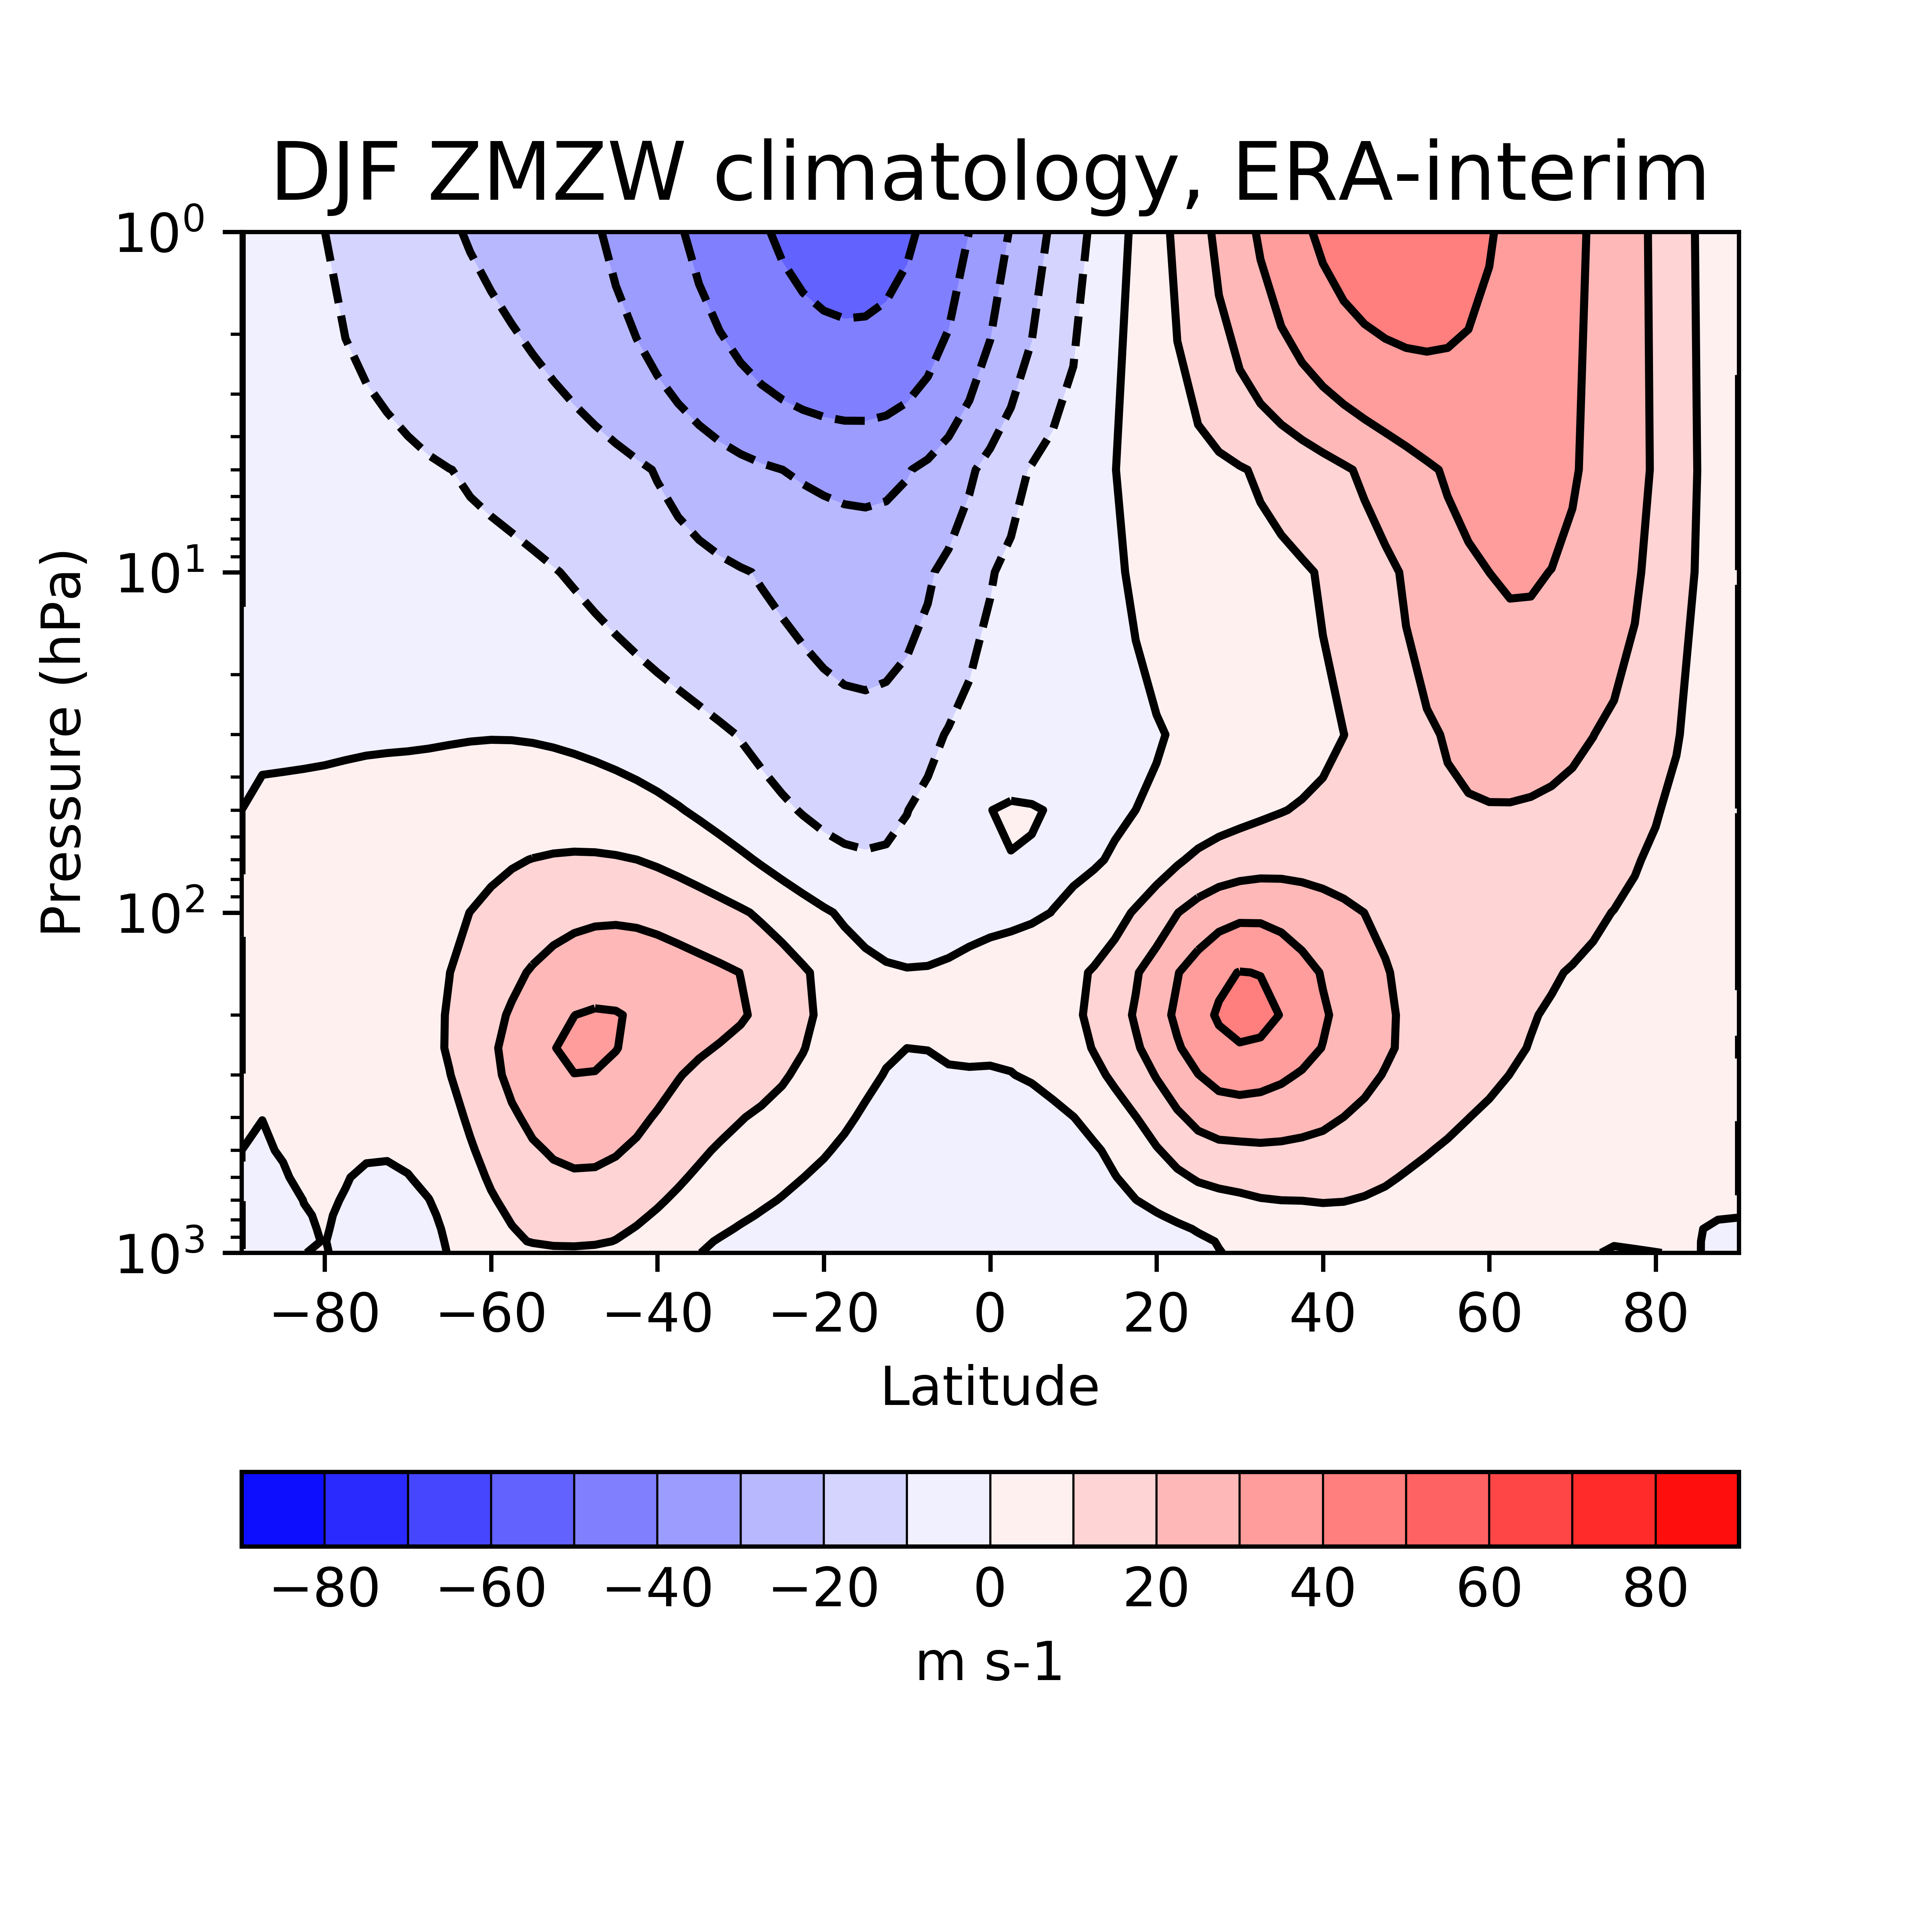
\includegraphics[width= 9cm]{Figures/Figures-background/fig1_for_transfer.png}
    \caption{DJF climatological zonal mean zonal wind from ERA-interim dataset between 1979 and 2018.}
    \label{fig:ERAclimDJF}
\centering
\end{figure}

\section{Atmospheric Waves}
\label{sec:atmos_waves}
Atmospheric wave is the term generally used for deviations from the zonal mean dynamical state and these phenomena, often referred to as Rossby waves, play a key role in the variability of the vortex. These waves are forced in the troposphere by air flowing over variations in topography (orographic waves) or through other mechanisms such as interaction with convection fronts and latent heat release (non-orographic). Perturbations originating near the surface can propagate vertically into the stratosphere altering large scale circulation features via wave drag as they transfer momentum to the background flow. 

Large scale Rossby waves are known as planetary waves and exhibit wavelengths of the order of $1000km$. The propagation of these waves can be described using the Quasi Geostrophic approximation for fluid in hydrostatic balance with low Rossby number, $R_0 = U/f_0 L$, where U and L are characteristic zonal velocity and length scales respectively. Under this framework the Quasi Geostrophic Potential Vorticity (QGPV) equation states that in the absence of friction and diabatic heating, the quasi geostrophic potential vorticity, $q$, is conserved following the geostrophic wind:

\begin{equation} \label{eq-PV_conserved}
D_g q = 0
\end{equation}

where $D_g$ is the operator 

\begin{equation}\label{eq:D_g}
D_g = \frac{\partial}{\partial t} + u_g \frac{\partial}{\partial x} + v_g\frac{\partial}{\partial y} 
\end{equation}

and $q$ can be written in terms of the stream function, $\psi$, in the QGPV framework as

\begin{equation} \label{eq:QGPV}
q = f_0 + \beta y + \nabla^2 \psi + \frac{\partial}{\partial z}\bigg(\frac{f_0^2}{N_B^2} \frac{\partial \psi}{\partial z}\bigg)
\end{equation}

where $N_B$ is the Brunt–Väisälä frequency, the frequency of vertical motion of a parcel of air in a stable atmosphere. $\psi$ is related to $u_g$ and $v_g$, the zonal and meridional components of geostrophic wind by $u_g = -\frac{\partial \psi}{\partial y}$ and $v_g = -\frac{\partial \psi}{\partial x}$. Under a further approximation of small disturbances from a uniform zonal flow, $\overline{u}$, $\psi$ is given by

\begin{equation} \label{eq:Zonal_flow_SF}
\psi = -\overline{u} y + \psi '
\end{equation}

where $\psi'$ is the contribution to the stream function from the small deviation from $\overline{u}$. This approximation allows equation \ref{eq:QGPV} to be linearised to

\begin{equation} \label{eq:Linearised_QGPV}
\bigg(\frac{\partial}{\partial t} + \overline{u} \frac{\partial}{\partial x}\bigg)\Gamma \psi' + \beta \frac{\partial \psi'}{\partial x} = 0,
\end{equation}

where $\Gamma$ is the operator

\begin{equation} \label{eq:ellipse_operator}
\Gamma = \nabla^2 \psi + \frac{\partial}{\partial z}\bigg(\frac{f_0^2}{N_B^2}\frac{\partial}{\partial z}\bigg).
\end{equation}

It can be shown that this equation has wave like solutions whose vertical propagation is only supported under the condition

\begin{equation} \label{eq:propagation_critera}
\overline{u} - c = \frac{\beta k}{k^2 + l^2 + \frac{f_0^2 m^2}{N_B^2}} < \overline{u}_c = \frac{\beta k}{k^2 + l^2}
\end{equation}

Where $\overline{u}_c$ is a critical velocity corresponding to the background flow when $m = 0$, $c$ is the phase speed and $k, l$ and $m$ are the meridional, zonal and vertical wavenumbers of the wave respectively. Also imposing that, as $m^2 > 0$, $\overline{u} - c > 0$ as well as assuming stationary waves ($c = 0$) gives the Charney-Drazin criterion for the vertical propagation of planetary waves,

\begin{equation} \label{eq:Charney-Drazin}
0 < \overline{u} < \overline{u}_c.
\end{equation}

This result implies that vertical propagation can only occur through background westerly zonal flow with a magnitude less than some critical value, $U_c$, which depends on the horizontal wavenumbers of the wave. More specifically, equation \ref{eq:propagation_critera} shows that smaller wave-numbers (larger wavelengths) favours greater propagation and is the reason the majority of wave-mean flow interactions involving the vortex occur with disturbances of wavenumbers 1-3 (referred to as wave-n disturbances). 

The Charney-Drazin criterion also leads to the definition of a critical layer of the atmosphere as the layer at which the background zonal flow no longer supports propagation of a given wave (i.e. where $\overline{u} \sim \overline{u}_c$). When a wave encounters a critical layer, much of the linear dynamical behaviour proposed in equations \ref{eq:Linearised_QGPV} breaks down as the waves' amplitude grows too large to support continued propagation and the wave dissipates, transferring momentum to the background flow through so called wave-mean flow interactions. There therefore exists a two way interaction between the background flow and wave disturbances in the atmosphere: the magnitude of $\overline{u}$ relative to $\overline{u}_c$ dictates the propagation of waves through the troposphere into the stratosphere and waves significantly influence the background wind upon dissipation at a critical layer.

Wave-mean flow momentum deposition which is key for understanding stratospheric dynamical variability can be quantified via the introduction of a variable known as the Eliassen-Palm flux. In the QG framework as above, equations for the zonal mean and eddy components of the wind vector ($u, v$) and buoyancy ($b$), the vertical acceleration of air parcels due to density variations, can be expressed as 

\begin{equation} \label{eq:QG_Ubar}
\frac{\partial \overline{u}}{\partial t} = f\overline{v} - \frac{\partial}{\partial y} \overline{u'v'} + \overline{X}, 
\end{equation}

\begin{equation} \label{eq:QG_theta}
\frac{\partial \overline{b}}{\partial t} = -N^2\overline{w} - \frac{\partial}{\partial y} \overline{v'b'} + \overline{Q}, 
\end{equation}

where the overbar denotes a zonal mean quantities and deviations from this (eddy quantities) are denoted by primes. $\overline{X}$ and $\overline{Y}$ represent the dissipative forces on the flow (in this case friction and diabatic heating). Buoyancy is used in these equations as a close analogous of temperature. $b = g\frac{T - T_r}{T_r}$ where $T_r$ is a reference temperature normally defined by height. $b$ is related to the concept of reduced gravity which is important when considering vertical fluid motion. 

In order to decouple these equations, we introduce the mean residual circulation, the difference between zonal mean flow and contributions from eddy-mean flow interactions. These are known as the Transformed Eulerian Mean (TEM) meridional and vertical velocities \citep{Andrews1976} (denoted by $^*$) and can be expressed as 

\begin{equation} \label{eq:V*}
\overline{v^*} = \overline{v} - \frac{1}{\rho_0}\frac{\partial}{\partial z} \bigg(\rho_0 \frac{\overline{v'\theta'}}{\frac{\partial{\overline{\theta}}}{\partial{z}}}\bigg)
\end{equation}\break
\begin{equation} \label{eq:W*}
\overline{w^*} = \overline{w} + \frac{\partial}{\partial y} \bigg( \frac{\overline{v'b'}}{\frac{\partial{\overline{\theta}}}{\partial{z}}}\bigg).
\end{equation}


Under these transformations the decoupled equations can be written as

\begin{equation} \label{eq:decoupled_U}
\frac{\partial \overline{u}}{\partial t} - f_0 \overline{v*} = \frac{1}{\rho_0} (\nabla \cdot F) + \overline{X}
\end{equation}

and

\begin{equation} \label{eq:decoupled_b}
\frac{\partial \overline{b}}{\partial t} + N^2 \overline{w*} = \overline{Q},
\end{equation}

where

\begin{equation} \label{eq:EP_flux}
F = -\rho_0 \overline{u'v'}\textbf{j} + f\rho_0\frac{\overline{v'\theta'}}{\frac{\partial{\overline{\theta}}}{\partial{z}}} \textbf{k}
\end{equation}

is the Eliassen-Palm flux which can be thought of as the flux of wave activity in the meridional and vertical directions (\textbf{j} and \textbf{k} represent unit vectors in the $y$ and $z$ directions) \citep{Andrews1976}. These equations indicate that EP flux divergence ($\nabla \cdot F > 0$) signifies momentum dissipation accelerating the ZMZW ($\overbar{u}$). Conversely, flux convergence ($\nabla \cdot F < 0$) indicates deceleration in ZMZW due to wave dissipation.

\subsection{Other Atmospheric Waves} \label{sec:other_waves}
In addition to planetary scale Rossby waves outlined in previous sections, other types of wave play a vital role in stratospheric variability. Gravity waves arise due to buoyancy variations and, similarly to planetary waves, can be forced through airflow over variations in topography (orographic) or convection fronts (non orographic). These waves exhibit length scales significantly shorter than planetary waves ($\sim xxxm$) and are often not explicitly represented in general circulation models (GCMs) due to horizontal resolution issues. Instead their effects are parameterised and appear in the dissipative force term ($\overline{X}$) in in equation \ref{eq:QG_Ubar}

Kelvin waves occur when air is trapped between regions in which Coriolis force terms act in opposite directions. In these regions, geostrophic balance does not apply and the waves exhibit a westerly phase velocity. Dissipation of these waves contributes westerly momentum to the background flow. Finally, Rossby-gravity waves exhibit different behaviour for small and large length scales (or horizontal wave number, $k$). for small $k$ (large length scale), they reduce to Rossby wavelike disturbances, similar to planetary scale Rossby waves outlined in the previous section in which variations in Coriolis parameter with latitude act as the restoring force. For large $k$ (shorter length scales), they behave as gravity waves (those for which the restoring force is gravity). Rossby-gravity waves typically have easterly phase velocity and contribute easterly momentum to background flow upon dissipation \citep{Andrews1976}.

\section{Sudden Stratospheric Warmings}
While the vortex generally exhibits strong, westerly flow over the boreal winter, it can be significantly disrupted on sub-seasonal timescales
(see individual season winds on figure \ref{fig:ERAclimDJF}b). This reversal occurs due to the dissipation of planetary waves on the vortex depositing easterly momentum on the background flow. If this deposition is large enough such that the vortex becomes significantly disrupted (and even reversed) an event known as a sudden stratospheric warming (SSW) occurs. Such events are named as they are often associated with significant and rapid increases in middle atmosphere polar cap temperature ($\sim~50K$ over a few days) and they were first observed in radiosonde data in Scherhag et al. 1952 (ref xxxx). In observation based datasets SSWs occur at an average rate of xxxx events per decade and represent one of the largest modes of interannual variability in the NH stratosphere.

Matsuno 1971 was the first work to introduce a dynamical model linking the action of planetary waves and the occurrence of SSWs. The framework developed by this work is still largely accepted today and describes the mechanisms involved in the life cycle of an SSW as follows: First, a burst of planetary wave activity is generated in the troposphere through a combination of airflow of topography and convection fronts. Waves subsequently propagate into the stratosphere in accordance with the Charney-Drazin criterion. When these waves encounter a critical layer (normally one which exhibits stronger westerlies than $\overline{u}_c$ as the undisturbed vortex is strong) these waves break and dissipate easterly momentum to the background zonal flow. As a result, the westerly vortex decelerates and, if stratospheric conditions are appropriate or the planetary wave activity is strong enough, even reverses. As a result, new critical layers are formed (where $\overline{u} = 0$) at a level below that of the original reversal. Subsequent waves now dissipate and can act to reverse the background flow at this lower critical layer. This process repeats and the critical layers can descend into the lower stratosphere. Once the critical layer lies near the tropopause, planetary waves are effectively prevented from entering the stratosphere stopping further deceleration of the vortex. With wave driving of the vortex prevented, radiative cooling of the stratosphere subsequently bring polar cap temperatures back down and the strong westerly flow of the vortex recovers. While this framework of dynamical processes involved in SSWs is relatively well accepted, there are contrasting hypotheses regarding the triggering mechanisms which initiate events. The primary mechanism suggested as the trigger is a rapid injection of wave activity from the troposphere which is large enough to significantly disrupt the vortex (Matsuno 1971; Limpasuvan et al. 2004; Manney et al. 2009; Nishii et al. 2009; Ayarzaguena et al. 2011; Kuttippurath and Nikulin 2012). An alternative hypothesis is that the state of the stratosphere itself also plays a key role in triggering events. Many studies support this phenomenon and have shown SSWs preceded by climatological wave driving from the troposphere which is subsequently amplified through non-linear resonance mechanisms with the stratospheric background flow (Esler and Scott 2005; Scott and Polvani 2006; Matthewman and Esler 2011; Esler and Matthewman 2011). 

The framework of Matsuno 1971 provides a mechanism by which SSWs occur through the interaction between planetary waves and the zonal mean background flow. However, further studies show that as well as zonal mean disturbance, the geometry of the vortex is altered significantly during these events and this provides a method of event classification (Lehtonen & Karpechko, 2016; Mitchell et al., 2011; Seviour et al., 2013). During events, the vortex can either be displaced from its stable centroid to a lower latitude (figure xxx b) or split into two daughter vortices each of which exhibits a core of high PV air (figure xxxxc). It's further shown in xxxx et al. that the type of deformation occurring broadly depends on the wavenumber of the dominant planetary waves involved with wave-1 disturbances more associated with displacement events and wave-2 with split events. Other studies utilising this vortex geometry approach note that SSWs are preceded by planetary wave breaking on the edge of the vortex in the so called "surf zone" which strips high PV air off the edge of the vortex thus sharpening its PV edge (McIntyre and Palmer 1983, 1984). Further works examine this phenomenon in the context of vortex preconditioning in which its geometry preceding SSWs promotes subsequent disruption. This geometry varies depending on whether the trigger for an event is considered as tropospheric wave bursts, in which case preconditions are generally a weak but westerly vortex which promotes propagation (Nishii et al. (2009) and Kuttippurath and Nikulin (2012),  Ayarzaguena et al. (2011)), or resonance with the stratospheric state in which case specific preconditions for split and displacement events are observed (Charlton and Polvani (2007), Bancala et al. (2012)). The framework provided by Matsuno et al. as well as insights from geometry analysis gives a picture of the processes involved in these remarkable dynamical events. The role SSWs play in 2 way stratosphere-troposphere coupling as well as their links to surface variability is discussed fully in section xxxx.

\section{The Equatorial Stratosphere}\label{sec:equatorial_strat}
Another region which exhibits key modes of stratospheric dynamical variability is to the equatorial region. The most notable of these modes are the quasi-biennial oscillation the zonal flow which varies with a frequency of approximately 28-29 months between the 100\,hPa and 10\,hPa levels and the semiannual oscillation of zonal wind which cycles more regularly with a frequency of 6 months around the 1\,hPa level (figure \ref{fig:QBO_SAO_ERA}) \citep{Baldwin2001}.

\begin{figure}[h!]
\centering
    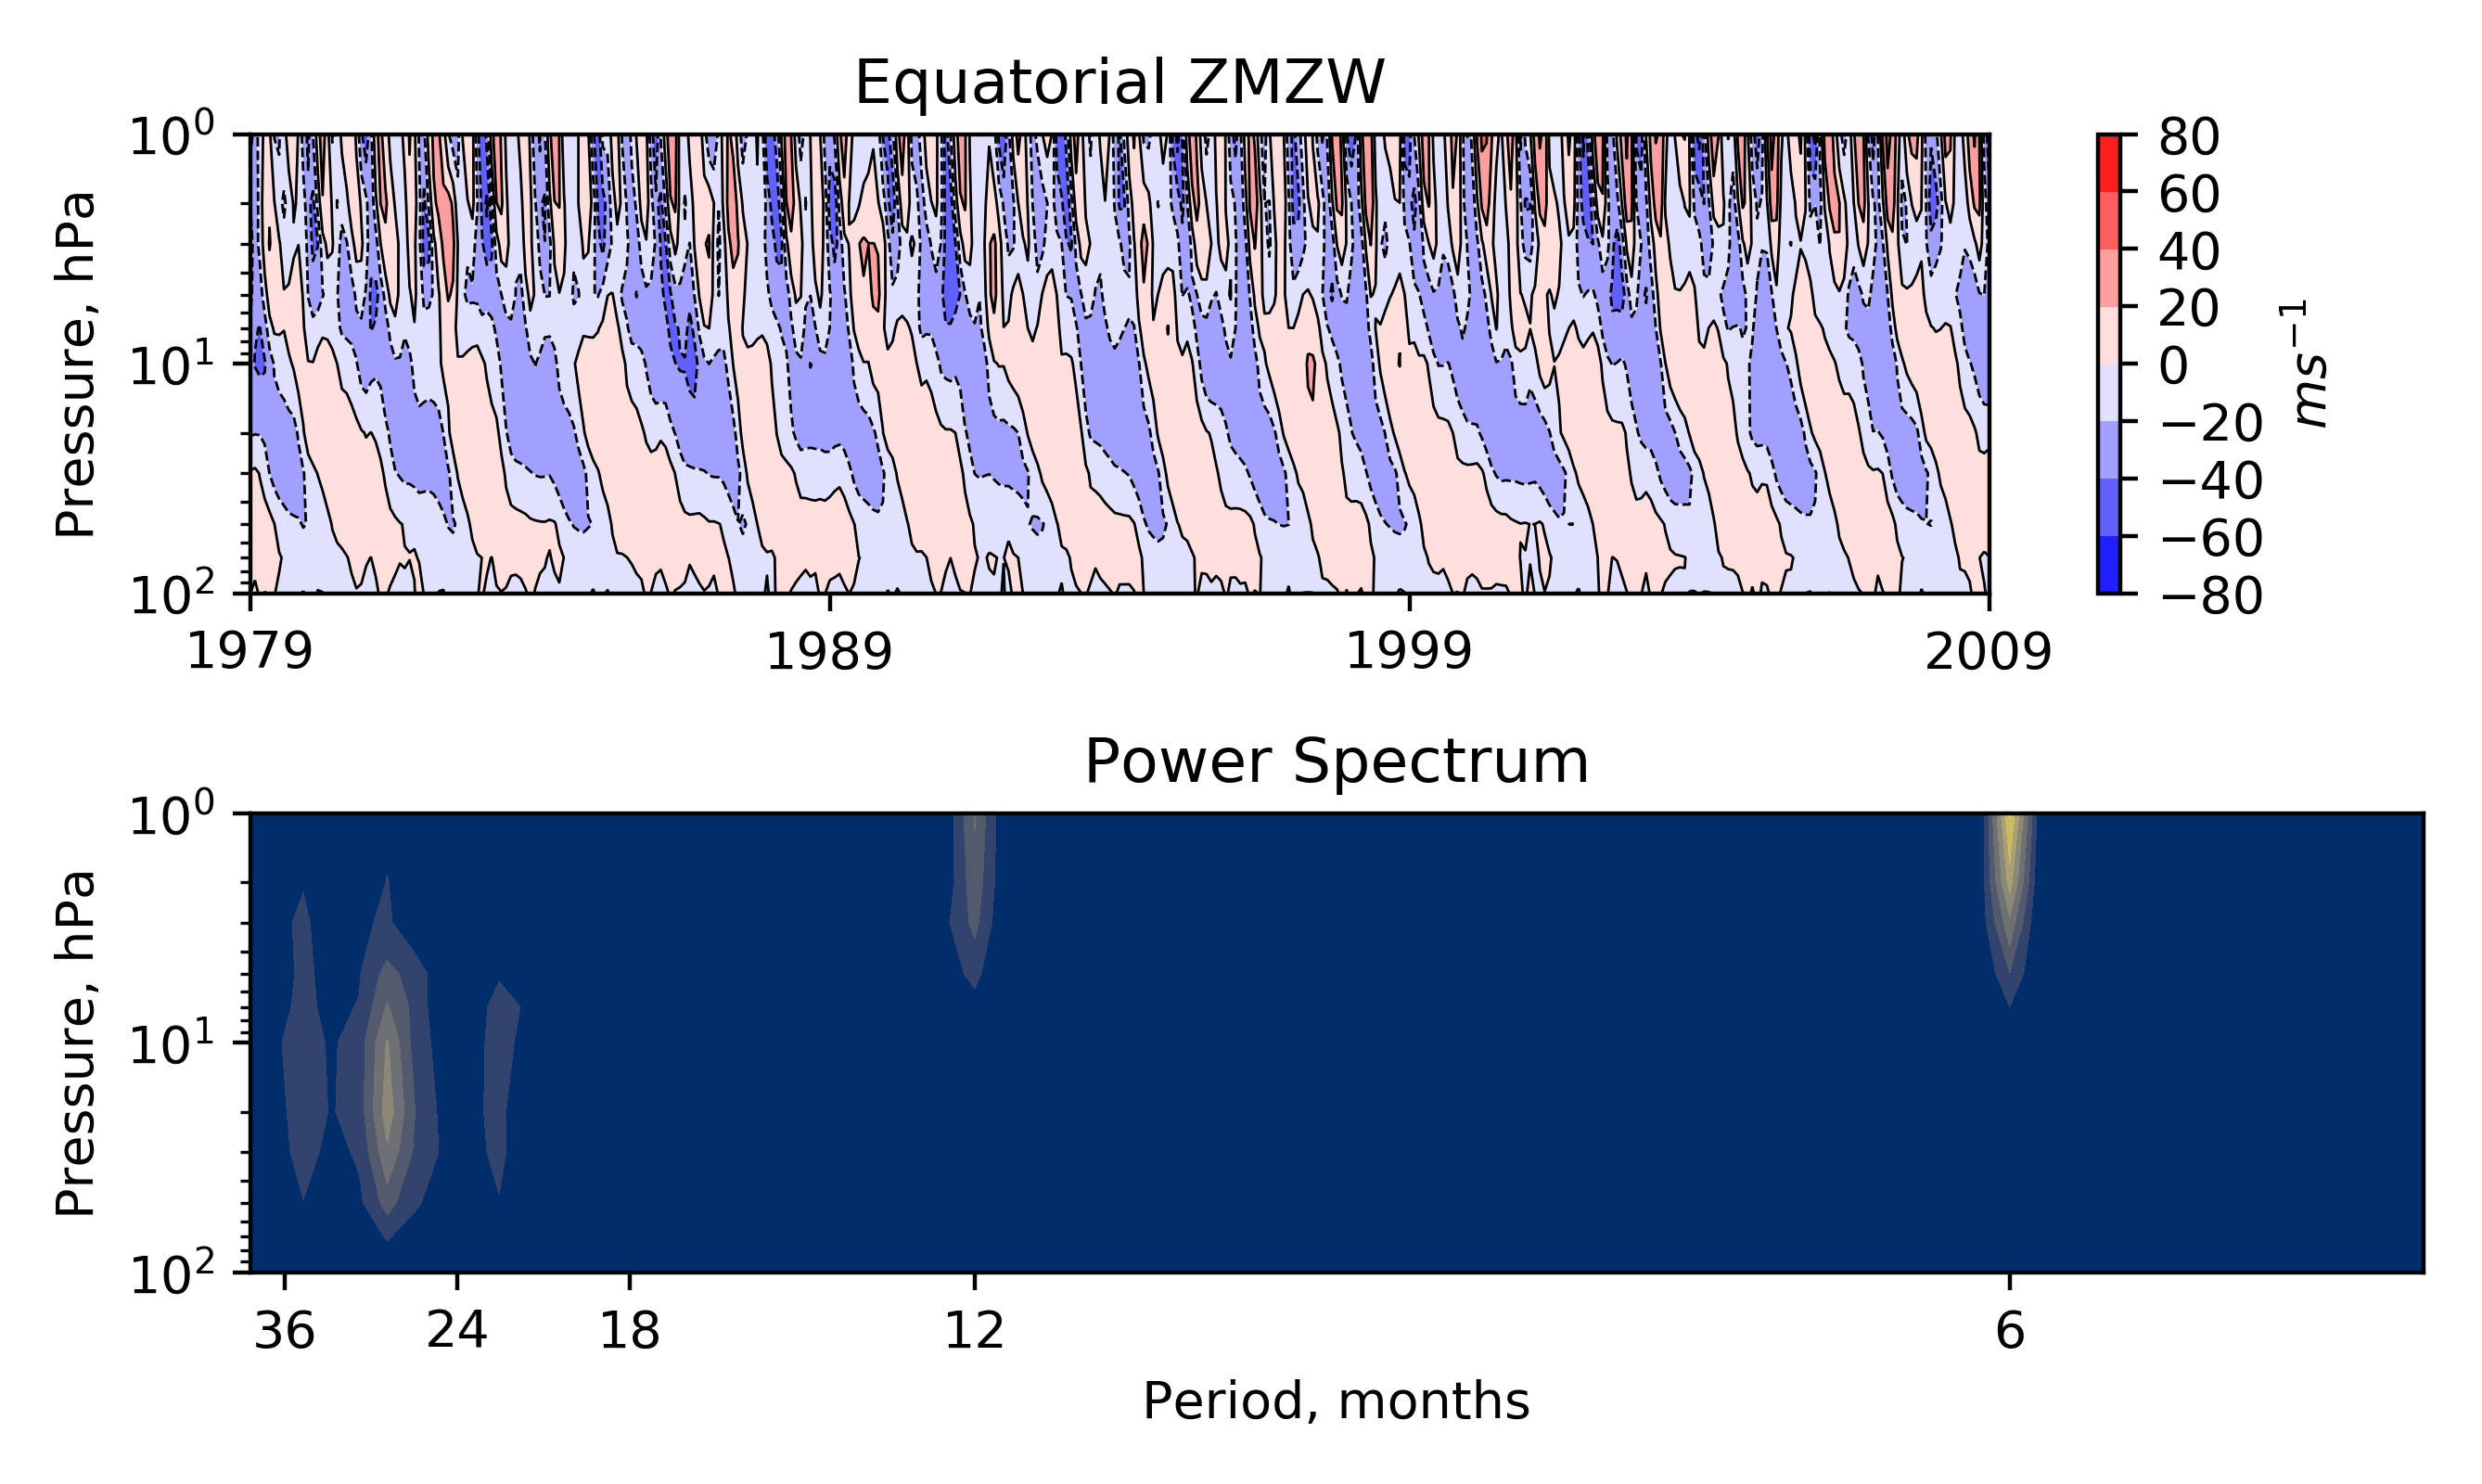
\includegraphics[width=0.88\textwidth]{Figures/Figures-background/QBO_SAO_ERA.png}
    \caption{Equatorial ZMZW (top) and associated Fourier power spectrum (bottom) for the ERA-Interim dataset between 1979 and 2009.}
    \label{fig:QBO_SAO_ERA}
\centering
\end{figure}
\FloatBarrier

The QBO was first fully classified as a phenomenon using balloon based observations in \cite{Ebdon1960} and \cite{Reed1964}. These studies found a set of descending shears of easterly and westerly ZMZW above the equator between approximately the 10hPa and 100hPa pressure levels. These seminal studies made use of a short observational record (approximately 5 years) and later works with more comprehensive observation based datasets were able to establish the key features of the oscillation \citep{Baldwin2001,Pascoe2005}. These include an approximate period of 28.1 months (although a range of 22-40 months is also recorded) with an asymmetry in the rate of descent of the westerly and easterly phases - slower descending easterly winds are caused by increased equatorial upwelling associated with this phase \citep{Pascoe2005}. The oscillation is generally zonally symmetric \citep{BELMONT1968} and has a latitudinal extent of approximately $12^{\circ}$ half width at half maximum \citep{Baldwin2001}.

The primary cause of the oscillation is the interaction of waves outlined in section \ref{sec:atmos_waves} with the background zonal flow. To analyse the action of these disturbances, it is useful to consider a pair of equatorial waves with phase speeds of $+c $ and $-c$ respectively (figure \ref{fig:QBO_wave_schematic}) \citep{Plumb1984}). These waves propagate or dissipate according to the difference between their phase speed and the background flow, $\overbar{u}$. If $\overbar{u}$ approaches $+c$ or $-c$ at a given height, the respective wave will deposit momentum of the same sign as its phase speed onto the background flow. This means that, for a background wind profile like that shown in \ref{fig:QBO_wave_schematic}a, westerly momentum is deposited at the bottom of a zone of westerly low altitude background wind, while easterly phase speed waves pass through and are deposited above on easterly flow. Viscous body acceleration counteract these wave accelerations leading to profiles in figure \ref{fig:QBO_wave_schematic}b where westerly waves pass through the flow and easterlies deposit momentum. Finally westerly waves begin to accelerate flow from high levels descending to finally force the background profile to figure \ref{fig:QBO_wave_schematic}d which is the inverse of schematic a. The asymmetry in descent speed between phases of the QBO is accounted for by the induced meridional circulation associated with each phase. An easterly QBO in the lower stratosphere induces a poleward meridional circulation at the same level \citep{plumb82,Baldwin2001} as well as an acceleration in upwelling over the equator, this slows the descent of the QBO easterlies \citep{Reed1964}. The converse is true for a westerly phase in the lower stratosphere. 

\begin{figure}[h!]
\centering
    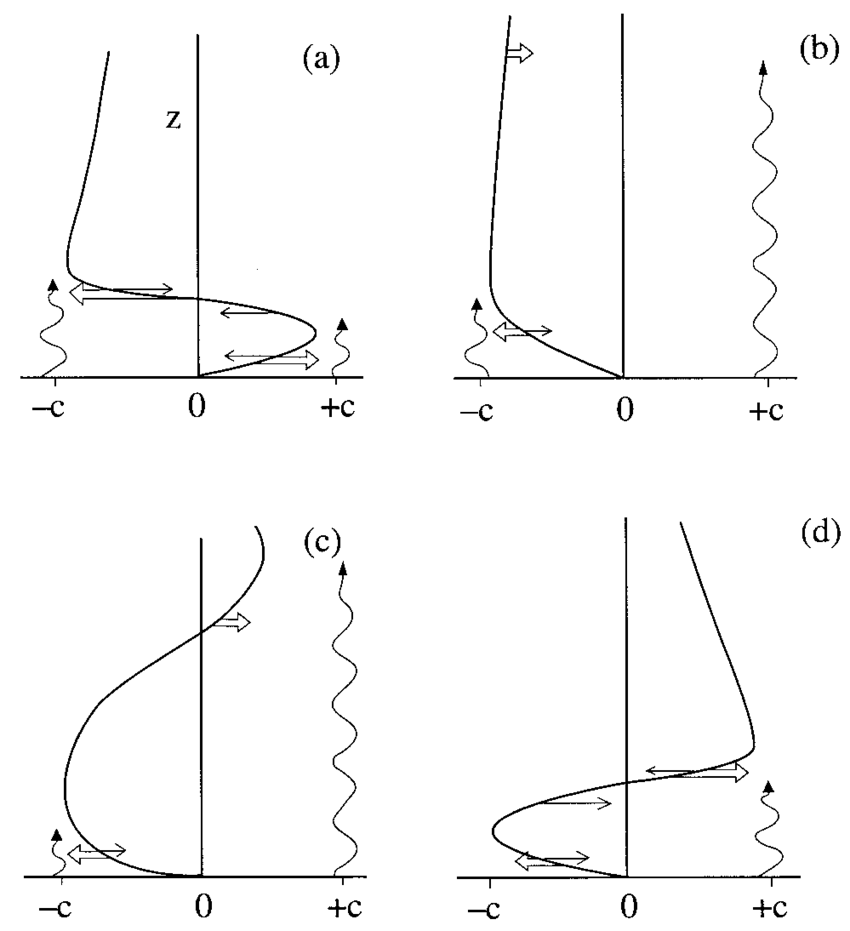
\includegraphics[width=0.5\textwidth]{Figures/Figures-background/Schematic_of_QBO_waves.png}
    \caption{Schematic of equatorial wave-mean flow interactions for 2 example wave disturbances (phase speeds $^+_- c$) from \cite{Plumb1984}. Solid continuous lines show the background flow of the QBO in developing phases, wavy arrows indicate propagation of the 2 waves, double arrows show momentum deposition on the mean flow from wave breaking, single arrows indicate viscous-driven acceleration.}
    \label{fig:QBO_wave_schematic}
\centering
\end{figure}

There exists a large body of literature examining the nature of the QBO; of particular relevance for the work presented in this thesis is how this mode associates with variability in the polar vortex. An association between the phase of the QBO and the strength of the polar vortex was first proposed by \cite{HoltonJamesRTan1980} and \cite{Holton1982} who found that the polar vortex exhibited a strengthening when the QBO near the 50\,hPa level was in its westerly phase (QBO-W) compared to its easterly phase (QBO-E). This link, usually referred to as the Holton-Tan (HT) effect, has been reported in subsequent studies with more comprehensive observations as well as in modelling studies using GCMs including the Met Office Hadley Centre Model 2 (HadGEM2) \citep{Watson2014} and other Met Office models \citep{Garfinkel2018}. Separate modelling studies also report a HT effect \citep{Baldwin1991,Pascoe2005,Lu2008}.

A number of physical mechanisms have been proposed to account for the observed coupling between the QBO and the vortex. Most notable is the hypothesis that during westerly phases, the zero wind line (the latitude at various heights at which the NH mid latitude winter westerlies meet the equatorial winds) is shifted equator-wards \citep{HoltonJamesRTan1980}. This can permit planetary waves to propagate vertically but be diverted equator-wards (according to the Charney-Drazin criterion, equation \ref{eq:Charney-Drazin}) and decrease their dissipative affect on the vortex. The converse argument can be made for easterly QBO phases when the zero-wind line lies further north and thus the planetary waves are guided more directly towards the vortex \cite{Lu14}. Indications of this effect may manifest in EP-flux divergence at different latitudes for each QBO phase however, studies which have tested this mechanism show varied results. \cite{Hamilton} finds a significant difference in latitudinal distribution of EP-flux divergence between QBO phases in accordance with the mechanism proposed above however \cite{Hu2002} and \cite{Gray2004} suggest the mechanism only takes effect during certain winter months. Furthermore \citep{Garfinkel12} present the idea of the HT effect competing with other phenomena such as the meridional circulation associated with QBO phases leading to variations in strength of QBO-vortex coupling. \cite{Lu14} examines this further and shows that the strength of the HT effect is transient in nature; the coupling is weakened if a broader and stronger vortex is present in NH winter due to divergence of wave activity generated by eddies within the vortex itself. This diverts wave activity equatorwards, an opposite driving mechanism to that of Holton-Tan. These competing processes temporarily reduces the influence of the QBO on the vortex.

The QBO is typically defined by the equatorial ZMZW at a single level in the mid-stratosphere. The 50 hPa level is usually used for NH observational studies \citep{Baldwin2001, Baldwin98} but some studies have also noted the importance of characterising the vertical structure of the QBO \citep{Fraedrih1993, Wallace1993,  Baldwin98,  Dunkerton2017, Gray2018, Andrews2019}. In an observational-based study \cite{Gray2018} find an enhanced association between the QBO and polar vortex when a metric incorporating the vertical coherence of equatorial winds via empirical orthogonal functions is utilised \citep{verena2016a}. In a model-based study \cite{Andrews2019} introduce a similar but simpler methodology by defining the QBO as the average ZMZW between two vertical levels, which preferentially selects time intervals that display a vertically coherent QBO phase between the specified levels. The same study reports enhanced responses to the QBO from the NAO and Arctic Oscillation (AO) when such vertically integrated metrics are used to define QBO phase compared to a single level definition. While these studies highlight statistical associations between vertical QBO metrics and the vortex, the importance of vertical coherence in HT strength has not been tested explicitly. Furthermore, influence mechanisms are not well understood. 


\section{Stratosphere-Troposphere Coupling and Surface Variability}
\section{Stratosphere-Ocean Interactions}



\chapter{Origins of Multi-decadal Variability in Sudden Stratospheric Warming events}
\label{cha:models}
\begin{quotation}
  Much of the work presented in this chapter is based on \cite{dimdore-milesOrigins2021} however the analysis has been extended here to include a more comprehensive diagnosis of stratospheric variability in the.
\end{quotation}


\section{Introduction}
\label{sec:origins_introduction}
Despite a significant body of work aimed at understanding the nature of vortex variability including SSWs, variations in this mode on decadal to multi-decadal timescales is not well understood. A formal diagnosis of such variability as well as a better understanding of factors which influence it may help to improve predictability of SSWs and subsequently NH mid-latitude surface climate \citep{Kidston2015}.

There is some evidence of vortex variations with periods longer than a year in the observational record. In reanalysis datasets, SSWs occur at an average rate of $\sim$0.6 events/winter but this varies markedly within the record \citep{butlerDefining2015b} suggesting the possibility of variability on much longer timescales. For example, observational studies have noted a hiatus in the 1990s when very few major SSW events occurred \citep{butlerDefining2015b,pawsonCold1999b, Shindell1999} while, in contrast, the early 21st century displayed a remarkable number of consecutive winters containing SSW events \citep{manneyRemarkable2005a}. Other studies have addressed the notion of low frequency variations in the vortex using GCMs. \cite{garfinkelStratospheric2017b} analyse decadal-scale variations in vortex strength in a set of historical simulations and propose that an observed hiatus in Eurasian surface warming was most likely due to variability in midwinter vortex strength. Similarly, \cite{cohenDecadal2009b} find decadal scale variations in planetary wave forcing of the vortex in a suite of CMIP3 models as well as NCEP–NCAR reanalysis. Whether the vortex variability was forced by greenhouse gas concentrations or arose through internal variability in these studies was not fully established but \cite{garfinkelEffect2015b} used a subset of the simulations analysed in \cite{garfinkelStratospheric2017b} and linked a decadal trend (1980-2009) in late winter vortex strength to SST variability. On the other hand, \cite{Seviour2017} analysed observed variations between 1980 and 2016 and concluded that the vortex variability was primarily internally generated. Other studies also point towards internally generated decadal fluctuations in vortex strength: \cite{manziniStratospheretroposphere2012b} explore causes of 20 year period variability in a simulation with prescribed, pre-industrial SSTs. They propose that, given the boundary conditions in the simulations are fixed, such variability must be internally generated. Finally, \cite{Butchart2000} suggest that decadal variability in vortex strength as well as SSW frequency may originate from feedbacks caused by the non linear nature of boreal winter stratospheric dynamics.

On longer timescales, \cite{schimankeMultidecadal2011b} note variations in SSW occurrence with periods of approximately 52 years in a multi-century GCM integration and demonstrated coherent variability in other parts of the climate system, including vertically propagating planetary wave activity, Eurasian snow cover and Atlantic SSTs. However, despite providing some indications of externally driven variability, results from this study are not conclusive, since the GCM used (EGMAM: ECHO‐G with Middle Atmosphere Model) exhibits significant bias in mean SSW rate compared to reanalyses (2 events per decade compare to $\sim$6 in reanalysis). The authors also note that further simulations are required to understand this variability. 

multi-decadal scale variations in climate features which can couple with the vortex has also been explored. There are clear decadal variations in the period and phase transition timing of the QBO \citep{pascoeQuasibiennial2005b,ansteyResponse2008b,Yang2016}. These may be linked to variations in the degree of 'stalling' of the QBO phase descent, which can cause more or less persistent wind direction at a given level.  A number of studies have also noted the transient nature of the strength of the HT relationship \citep{luDecadalscale2008c,luMechanisms2014c,ansteyResponse2008b,ospreyClimatology2010b}. \cite{luDecadalscale2008c,luMechanisms2014c} show that the mid-latitude wave-guide is modulated by the shape of the vortex so that planetary waves are diverted further equatorwards when the vortex is anomalously strong and wide, and this could temporarily reduce the influence of the QBO on the vortex. The Aleutian Low (see section \ref{sec:external_influence_AL}) also varies significantly on decadal to multi-decadal timescales. \cite{overlandDecadal1999b} note that 10 year mean values of SLP over the AL region exhibit fluctuations of up to 35\% of the climatological mean. Subsequent studies corroborate the presence of these decadal scale fluctuations: \cite{SUGIMOTO2009} and \cite{Minobe} show 20 year fluctuations in intensity and centre of action of the AL while \cite{Raible2005} propose a 50-60 year trend in AL intensity, suggesting the existence of even longer timescale variability. 

Although substantial effort has been applied to characterising SSWs and their underlying mechanisms, there is little understanding of periods of hiatus (such as that in the 1990s) and consecutive-event years (early-mid 2000s), primarily because of the short record of reliable observations as well as the complexities and often non-stationary nature of the multiple observed teleconnections. Much longer time-series are required to successfully identify and understand the source of decadal and multi-decadal scale variability. In the meantime, analysis of variability and teleconnections in long climate model simulations may help to understand these processes. 

In this chapter, we analyse long-term variability of the stratospheric polar vortex in a 1000-yr pre-industrial (pi-cntrl) simulation of the UK Earth System Model (UKESM). The absence of external forcings such as greenhouse gas increases, volcanic and solar variations allows us to examine sources of long-term variability that are internally generated within the climate system. We identify intervals containing high and low SSW rates and analyse their variability, with a focus on multi-decadal scales. A variety of techniques are employed to examine associations with those parts of the climate system that are known to exhibit long-term memory, namely the tropical SSTs and the AL. In particular, a wavelet spectral decomposition and cross-spectrum analysis is employed to overcome some of the difficulties with non stationary signals that may arise. We also investigate interactions between the vortex and the QBO as a potential source of internally-driven variability.

\section{Data And Methods}

\subsection{Model Configuration}
\label{sec:model_config}
For analysis of multi-decadal variability in the vortex and SSWs, we utilise a simulation of the first version of the UK Earth System Model (henceforth referred to as UKESM), a configuration of the MetOffice unified model (the UM) \citep{mulcahyImproved2018b}. UKESM is a stratosphere resolving coupled ocean-atmosphere-land-sea ice model. The Atmospheric component is GA7.1 with 85 vertical levels from the surface to 85km, 35 of which are above 18km \citep{waltersMet2019b, williamsMet2018b}. The model is run at N96 horizontal resolution (approximately 135 km near the equator). The ocean model used is GO6.0 \citep{Storkey2018} which contains 75 levels and runs at 1${^\circ}$ horizontal resolution. Land surface and sea-ice processes are represented by JULES \citep[GL7.0,][]{waltersMet2019b} and CICE  \cite[GSI8.1,][]{ridleySea2018b} models respectively, while ocean biochemistry is added through MEDUSA \citep{Yool2013}. UKESM also includes a fully interactive chemistry scheme via coupling with the UK Chemistry and Aerosols model \citep[UKCA,][]{mulcahyImproved2018b}.

We utilise a 1000 year pre-industrial (PI) control simulation of UKESM submitted to CMIP6 which is spun-up to achieve initial model equilibrium following the method outlined in \cite{yoolSpinup2020b}. This run is forced using CMIP6 pre-industrial values for concentrations of major GHGs (global mean 284.317ppm $CO_2$, 808.25ppb $CH_4$, 273.02ppb $N_2O$). While there are no volcanic eruptions in the simulation, background stratospheric volcanic aerosols are set to climatological values between 1850 and 2014 estimated from satellite products and other model simulations \citep{menaryPreindustrial2018b}. We choose a PI control for this analysis to examine internal variability in SSWs on multi-decadal timescales. 

\subsection{Reanalysis Data}
\label{sec:ERA_data}
To verify that the model reproduces relevant features of the climate system we compare with an observation based dataset produced by the ECMWF - ERA-Interim \cite{Dee2011}. The ERA-interim dataset is produced by a 4D-Var data assimilation method of a wide range of observations \citep{Uppala2005}. These include surface measurements, aircraft campaign data, radiosonde readings and satellite observations. The 4D-var data assimilation process involves supplying the ECMWF’s Integrated Forecast System (IFS) initial conditions from observations, letting the model evolve for a timestep and re-initialising for the next step with a combination of output and updated observations \citep{courtierECMWF1998, bouttierObservingsystem2001a}. This update is carried out to minimise a cost function defined to capture the difference between the latest model output and observations for that corresponding time. ERA-Interim provides data on 60 vertical levels at a maximum horizontal resolution of $\sim$ 80 km from 1979-2019 \citep{Berrisford}.

The majority of observations assimilated for ERA-Interim are satellite based radiance retrievals. These are gained from nadir facing satellites which measure spectral radiances (energy detected at difference wavelengths). A single detection device will consist of several channels which detect radiation from difference wavelengths. Different atmospheric layers absorb and emit at different wavelengths so measuring over a range of channels can build up a vertical profile of a variable such as temperature. However, the atmospheric layers that are detected by each channel may overlap resulting in measurements from multiple channels being used in the retrieval of a given layer. A weighting is applied to the channels at each height to account for the proportion of the total measurement that should be contributed by each channel. Channel weighting profiles (see figure \ref{fig:Satellite_channels}) are generally Gaussian (for Nadir Satellites) in pressure coordinates \citep{fujiwaraIntroduction2017}, the width of which signifying the vertical extent of the channel. The vertical resolution of the retrievals is determined by the density of channels covering a particular height range. 

During the ERA-Interim period, the set of observations used for assimilation have developed significantly. Between 1979 and 1998 only limited satellite based radiance retrievals are available to produce profiles. These satellite observations are primarily provided by the Stratosphere Sounding Unit (SSU) and Microwave Sounding Unit (MSU) which are parts of the TRIOS Operational Vertical Sounder (TOVS) suite. The SSU possesses only 3 channels (figure \ref{fig:Satellite_channels}a) and therefore provides data at relatively coarse vertical resolution. Over this period, ERA-interim relies heavily on direct measurement techniques such as radiosondes, dropsondes and aircraft \citep{fujiwaraIntroduction2017} which bring possible biases from the influence of shortwave solar heating on temperature sensors in radiosondes as well as warmer tendencies in aircraft based observations compared to radiosondes \citep{ballishSystematic2008}. After 1998 more extensive satellite based measurements are available for assimilation and are incorporated in ERA-interim. The new satellite products include improved versions of the SSU and MSU as a part of the Advanced TRIOS Operational Vertical Sounder (ATOVS) suite which provides profiles derived from the Advanced Microwave Sounding Unit A (AMSU, figure \ref{fig:Satellite_channels}b) from which ERA-interim calculates profiles using 11 channels (channels 5-14 from AMSU). ERA-Interim also makes use of a number of other satellite based instruments which are fully outlined in \citep{fujiwaraIntroduction2017}. Possible sources of biases in these satellite based observations include orbital drift and calibration offsets \citep{simmonsEstimating2014}.

As a result of including additional observations for assimilation after 1998, ERA-interim shows a shift in temperature structure of the middle and upper stratosphere between the two periods. Caution is therefore advised when using this data for trend analysis \citep{longClimatology2017} however such an analysis does not form part of the work in this thesis. Zonal wind fields show little change across the periods. Additionally, ERA-interim struggles (as the majority of modern reanalyses do) to constrain phase transition timing of the QBO correctly \citep{kawataniRepresentation2016}. Comparisons with wind profiles derived from a single radiosonde station (Singapore at $^{\circ}$1N, $104^{\circ}$E), which covers a large majority of the reanalysis period, show that ERA-interim also exhibits biases in the amplitude of both QBO phases. These biases reduce significantly with the transition to the use of ATOVS \citep{kawataniRepresentation2016,longClimatology2017}. Similar biases and improvements over the TOVS-ATOVS period are also observed for representation of the SAO \cite{baldwinTropical2005}. These biases must be taken into account when considering comparisons in stratospheric circulation between ERA-interim and GCMs. Nonetheless, \cite{longClimatology2017} stress that these datasets are in broad agreement with other major reanalyses in the stratosphere and lower mesosphere.

\begin{figure}[h!]
\centering
    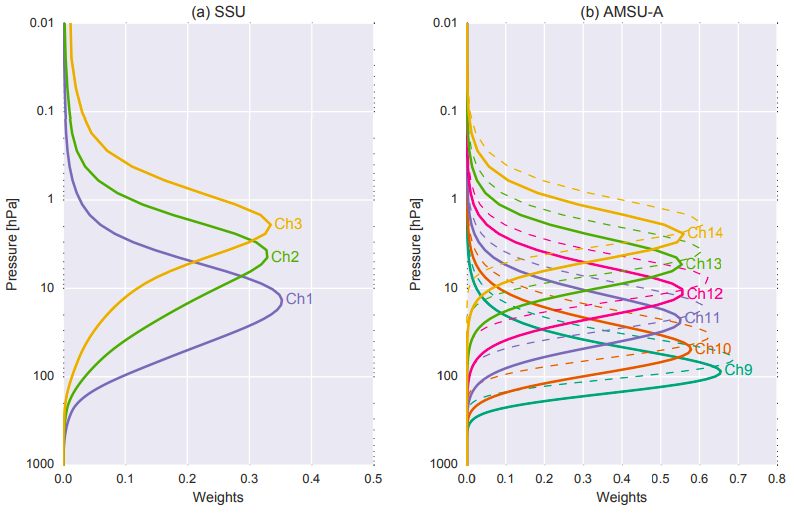
\includegraphics[width=0.85\textwidth]{Figures/Figures-origins/channels.png}
    \caption[Channel profiles for satellite retrievals assimilated by ERA-Interim]{Figure from \cite{fujiwaraIntroduction2017} \textbf{Left}: Channel weighting profiles for the TOVS Stratospheric Sounding Unit (SSU) used for ERA-Interim dataset in the period 1979-2005. \textbf{Right}: Weighting profiles from the ATOVS-suite Advanced Microwave Sounding Unit (AMSU) which provides measurements for ERA-Interim from 1998-present. Solid lines represent near Nadir profiles and dashed lines signify limb profiles (taken at an angle of $48.33^{\circ}$).}
    \label{fig:Satellite_channels}
\centering
\end{figure}

\subsection{Wavelet Analysis}
\label{sec:Wavelet_Analysis}
In order to study possible multi-decadal variability in SSW occurrence, we utilise a wavelet analysis method based on \cite{Torrence1998}. Such an analysis can be used to examine time series which displays non-stationary spectral power over multiple frequencies \citep{Daubechies} giving it a useful advantage over more traditional fourier methods for spectral analysis. The wavelet transform of a uniform 1-dimensional time series, $x$, of length $N$ and timestep $\delta t$ is given by the convolution between the series and a scaled and translated version of a wavelet function $\psi_0$ (equation \ref{wavelet_transform})

\begin{equation} \label{wavelet_transform}
W_n(s) = \sum^{N - 1}_{n' = 0} x_{n'} \psi^* \bigg[(n' - n) \frac{\delta t}{s}\bigg],
\end{equation}

\noindent where $*$ denotes the complex conjugate and $s$ is the wavelet scale indicating the frequency of the wavelet. Varying $s$ and translating along the time scale (the index $n$), $W_n$ indicates the amplitude of signals at different scales and their variation in time. \cite{Torrence1998} suggest an approach to varying the scale s as increasing in powers of 2 according to 

\begin{equation} \label{S}
s_j = s_0 2^{j \delta j},\\ j = 0, 1, ..., J
\end{equation}

\begin{equation} \label{J}
J = \delta j^{-1} log_2\bigg(\frac{N \delta t}{s_0}\bigg),
\end{equation}

\noindent where $s_0$ is the shortest resolvable scale of a signal, J corresponds to the longest and $\delta j$ is the scale resolution. The translated and scaled wavelet has the form

\begin{equation} \label{wavelet}
\psi^* \bigg[(n' - n) \frac{\delta t}{s}\bigg] = \bigg(\frac{\delta t}{s}\bigg)^{1/2} \psi_0\bigg[(n' - n) \frac{\delta t}{s}\bigg]
\end{equation}

\noindent and we select the form of $\psi_0$ following the recommendation of \cite{Torrence1998} as a Morlet wavelet, an oscillatory function enveloped by a Gaussian which is expressed as

\begin{equation} \label{psi0}
\psi_0(p) = \pi^{-1/4} e^{i\omega_0 p} e^{\frac{p^2}{2}}.
\end{equation}

The advantages of using a Morlet wavelet for analysing signals in climate time-series is discussed in \cite{lauClimate1995b} in which the authors acknowledge that, while truly physical signals should be detected regardless of which wavelet basis is chosen, for best results one should adopt a wavelet function reminiscent of the real signal. They show that when a Morlet wavelet form is utilised, spectral decomposition methods can detect common forms of behaviour exhibited in the variability of time series associated with the Earth's climate. These include time variations in period and amplitude of signals, abrupt changes in periodicity (sudden regime shift to different spectral behaviour) and some forms of rapid changes in series over time. These forms of behaviour are most likely relevant for our analysis of SSWs, therefore we proceed with a wavelet of this form. 

It is computationally quicker to compute the wavelet transform in discrete Fourier space. By the convolution theorem, the transform reduces to multiplication

\begin{equation} \label{wavelet_transform2}
W_n(s) = \sum^{N - 1}_{k = 0} \hat{x}_{k} \hat{\psi}^* (s\omega_k) e^{i \omega_k n \delta t},
\end{equation}

\noindent where $\hat{x}_{k}$ and $\hat{\psi}$ are the discrete Fourier transforms of the time series $x$ (equation \ref{fourier1}) and the wavelet function (equation \ref{fourier2}) respectively. These quantities are given by 

\begin{equation} \label{fourier1}
\hat{x}_k = \frac{1}{N} \sum^{N-1}_{n = 0} x_n e^{\frac{-2\pi i k n}{N}}
\end{equation}

\begin{equation} \label{fourier2}
\hat{\psi}(s\omega_k) = \bigg(\frac{2 \pi s}{\delta t}\bigg) \pi^{-1/4}H(\omega_k) e^{-(s\omega_k - \omega_0)^2/2}
\end{equation}

\noindent where $H(\omega_k)$ is the Heavyside function and $\hat{\psi}$ is normalised to have unit energy when integrated over all $\omega$. The square modulus of the wavelet transform gives the wavelet power spectrum which indicates relative strength of signals in the time series as a function of signal period and discretised time. In order to directly compare spectra of different indices we normalise all timeseries by subtracting the mean and dividing by its standard deviation before performing the wavelet transform. In order to effectively compare spectral power across a range of frequencies we additionally scale the power spectrum by dividing by the scale parameter ($s_j$ defined above) associated with each frequency. This is done following the methodology of \cite{liuRectification2007} which shows that un-scaled spectra exhibit a bias towards overestimated powers at longer periods and that an effective comparison across timescales is possible with such scaling. We also define a confidence interval for wavelet power observed at a given period and time for a series by assuming a mean background spectrum corresponding to that of a first order autoregressive (AR1, red noise) process modelled by

\begin{equation} \label{rednoise}
x_n = \alpha x_{n - 1} + z_n,
\end{equation}

\noindent where $\alpha$ is the lag-1 autocorrelation of the time series and $z_n$ is Gaussian white noise. \cite{Torrence1998} show that such a process's wavelet power spectrum is $\chi^2$ distributed and therefore can be used to define a 95\% confidence interval for any observed power. 

\subsection{Cross Wavelet Spectra}
The cross wavelet spectrum of two time series $x$ and $y$ with associated wavelet spectra $W^x_n$ and $W^y_n$ gives a measure of coincident power (the same period at the same timepoints) between the series. It is given by

\begin{equation} \label{wavelet_cross}
\vert W^{xy}_n(s)\vert = \vert W^{x*}_n(s) W^{y}_n(s)\vert,
\end{equation}

\noindent where $W^{x*}_n(s)$ is the complex conjugate of the wavelet power spectrum of $x$ \citep{grinstedApplication2004b}. The complex argument of $W^{xy}_n(s)$ gives the local phase difference between signals in $x$ and $y$ in frequency-time space. The phase relationship between the two time-series can be represented by a
vector that subtends an angle representing the phase difference: On all plots of cross spectra, arrows to the right (left) denoted signals which are in-phase and correlated (anti-correlated). Vertical arrows indicate a phase relationship of $\frac{\pi}{2}$ between the time-series, so that the evolution of
one is correlated with the rate-of-change of the other. As for individual power spectra, we define a confidence interval for which cross power of a larger amplitude is deemed significant (>95\% confidence interval) by comparing power exhibited by actual series with a theoretical red noise process. The cross power of two such AR1 processes is theoretically distributed such that the probability of obtaining cross power greater than a set of red-noise processes is

\begin{equation} \label{wavelet_cross_dist}
D\bigg(\frac{\vert W^{xy}_n(s)\vert}{\sigma_x \sigma_y} < p\bigg) = \frac{Z_\nu(p)}{\nu} \sqrt{P^x_k P^y_k},
\end{equation}

\noindent where $\sigma$ denotes the standard deviation of the time series, Z is the confidence interval defined by $p$ ($Z$ = 3.999 for 95\% confidence), $\nu$ is the degrees of freedom for a real wavelet spectrum ($\nu$ = 2) and $P^x_k$ is the theoretical Fourier spectrum of the AR1 process. For a given wavenumber k, this can be expressed as

\begin{equation} \label{theoretical_fourier}
P_k = \frac{1 - \alpha^2}{\vert 1 - \alpha e^{2i\pi k} \vert^2}.
\end{equation}

\subsection{Hilbert Transform}
We utilise a signal processing method known as a Hilbert transform to calculate the instantaneous phasor amplitude of a QBO time series. The Hilbert transform of a time series $x(t)$ can be expressed as

\begin{equation} \label{eq:hilbert1}
\tilde{x} = Hil[x(t)] = \frac{1}{\pi t} * x(t),
\end{equation}

\noindent where $\tilde{}$ denotes the transformed series, * signifies a convolution and $t$ is discretised time. Conversely, the original time series can be recovered using an inverse transform expressed as

\begin{equation} \label{eq:hilbert2}
{x(t)} = Hil^{-1}[\tilde{x}(t)] = -\frac{1}{\pi t} * \tilde{x}(t).
\end{equation}

A complex signal which consists of $x(t)$ and its transform is known as the analytic signal of $x$ and can be used to calculate an instantaneous phasor amplitude, $A(t)$, of the signal. $X(t)$ can be expressed as

\begin{equation} \label{eq:hilbert3}
X(t) = x(t) + \tilde{x}(t) i = A(t) e^{i\theta},
\end{equation}

\noindent where $A(t)$ is the instantaneous amplitude of the signal and $\theta(t)$ is the instantaneous phase angle - a measure of signal progression through a cycle at time $t$.

\subsection{Statistical Methods}
\label{sec:stat_methods}

\subsubsection{Student's t-test}
Much of the analysis presented in this chapter, and indeed in the whole thesis, involves comparisons of composite and mean quantities. A two-tailed student's t-test is implemented to test the null hypothesis that two sampled quantities, $x_1$ and $x_2$, with means $\overline{x}_1$ and $\overline{x}_2$ and standard deviations $\sigma_{1}$ and $\sigma_{2}$ are drawn from the same underlying normal distribution. A $t$ statistic is defined by $t = \frac{\overline{x}_1 - \overline{x}_2}{\sigma_{12} \sqrt{\frac{1}{n_1} + \frac{1}{n_2}}}$ where $n_i$ is the number of samples for quantity $i$ and $\sigma_{12}$ is the pooled variance for the two quantities given by $\sigma_{12} = \sqrt{\frac{\sigma^2_2 (n_2-1) + \sigma^2_1(n_1 - 1)}{n_1+n_2-2}}$. Significance on the difference in means can then be estimated by comparing the value of $t$ with a Student's t-distribution to give an associated $p$ value. Differences which give a $p$ value greater than a deemed level (normally 95\%) are deemed significant in which case the null hypothesis of identical means is rejected to this level.

\subsubsection{Linear Regression Analysis}
We employ a multi-linear regression technique to give an estimate of the relative contributions to SSW variability from the QBO, ENSO and the AL following the method outlined in \cite{Krzywinski}. We model an SSW timeseries of length $n$ which we denote $y$ as 

\begin{equation} \label{regression}
\hat{y} = \beta_0 + \beta_{1}QBO + \beta_{2}ENSO + \beta_{3}AL,
\end{equation}

\noindent where $\beta_j$ denotes the coefficient of the corresponding index and $\hat{y}$ is the prediction of $y$. We calculate the best estimate for each $\beta$ using an ordinary least square (OLS) estimator which minimises the sum of squared error (SSE) between the predicted $\hat{y}$ and the real time series $y$ with respect to each coefficient. the SSE is given by $SSE = \sum_i^n{(\hat{y}_i - y_i)^2}$ \citep{kimStatistical2018}.

We can compare the estimated magnitude of the coefficient for each index to analyse the respective contributions to SSW variability. We can also calculate standard error ranges for $\beta$ estimates. The standard error on an estimated value of a true $\beta_j$ (denoted by $\hat{\beta_j}$) is given by 

\begin{equation} \label{regression_se}
se(\hat{\beta_j}) = \sqrt{\frac{SSR}{n - k} (X^TX)^{-1}_{jj}},
\end{equation}

\noindent where SSR is the sum of squared residuals which measures the sum of squared deviations of predicted values from the mean $y$ value, $\overline{y}$. This is given by $SSR = \sum_i^n{(\hat{y}_i - \overline{y})^2}$). $k$ is the number of predictors used in the linear model (in this case 3) and $X$ is an $n \times k$ matrix consisting of the predictor indices. We also define significance levels for $\hat{\beta_j}$ using a one-tailed $t$ statistic (similar to above) with $n-k$ degrees of freedom to test the null hypothesis that $\hat{\beta_j}$ = 0. The $t$ statistic is given by $t = \frac{\hat{\beta_j}}{se(\hat{\beta_j})}$. We also define the coefficient of determination, $R^2$, of the model which gives the proportion of the variance in the dependant variable (in this case the SSW time series) accounted for by the contributions from the predictor indices (multiplied by their respective coefficients).

A potential pitfall of implementing this regression analysis is the possibility of significant covariations between predictor indices. If the variance of a given predictor is increased due to covariability with other independent variables, the standard error on the coefficient's estimate, $se(\hat{\beta_j})$, may be artificially inflated leading to difficulties in deriving meaningful findings from the model. A method for quantifying the severity of this multicolinearity issue for a given regression model is the variance inflation factor (VIF) \citep{akinwandeVariance2015b}. $VIF_j$, indicates the degree to which $se(\hat{\beta_j})$ is increased through the effects of all other predictors. It is given by $VIF_j = \frac{1}{1 - R_j^2}$ where $R_j^2$ is the coefficient of determination of a separate linear regression model with predictor $j$ (the AL, for example) as the dependant variable and all other predictors from the original regression model as the independent variables. For the example of the AL (j = 3), this model is given by

\begin{equation} \label{regression_vif}
AL = k_1 QBO + k_2 ENSO,
\end{equation}

\noindent where $k1$ and $k2$ are the estimates on coefficients of the secondary model. A value of $VIF_j > \sim 5$ indicates that multicolinearity has significantly increased the standard error on the estimate for $\beta_j$ and that the estimates of coefficients for the original model may be compromised by this effect. A $VIF_j > 1$ indicates a marginal effect from multicolinearity. 

\subsubsection{EOF Analysis}
\label{sec:eof_analysis}
We also utilise a method for diagnosing patterns of variability in a quantity defined on a spatial and temporal grid. Such a method, known as Empirical Orthogonal Function (EOF) analysis decomposes a function, $y$, into a set of basis functions which indicate the spatial patterns that maximises variance in $y$. 

if $y$ is defined on $N$ time points and $M$ spatial points then the time anomalies of $y$, defined as $y' = y - \overline{y}$ ($\overline{y}$ = the time mean of $y$ at each spatial point) can be expressed as an $N \times M$ matrix denoted as $Y$. The EOFs, $e_n$, are subsequently defined as the eigenvectors of the covariance matrix of $Y$, $C = \frac{1}{N-1}Y^TY$, such that $C e_n = \lambda_n e_n$. $\lambda_n$ is the eigenvalue which can be used to give an indication of the proportion of total variance in $y$ explained by the EOF $e_n$. Such a metric, the variance fraction, is given as $v_n = \frac{\lambda_n}{\Sigma_i \lambda_i}$ - the ratio of a given eigenvalue to the sum of all eigenvalues. EOFs are ordered by eigenvalue size such that EOF1 explains the largest fraction of the total variance. Projecting the matrix $Y$ back onto a given EOF, $e_n$, gives the $n^{th}$ Principle Component (PC) timeseries given by $PC_n = Y e_n$. For the majority applications of EOF analysis for diagnosing climate variability, the first 2 EOF patterns sufficiently explains the variance in quantities such as mean sea level pressure (MSLP) or geopotential height. In the work presented here, we utilise EOF and PC analysis to construct climate variability indices such as the NAM, NAO and AL.  

\subsubsection{SSW Statistics}
\label{sec:SSW_stats}
In order to assess model representation of vortex variability, we introduce a statistical framework which uses parametric and bootstrapping methods to asses significance levels for differences in SSW abundance across datasets. First, a parametric approach which assumes that the occurrence of any number of SSWs (denoted as $N$) in a given number of winters (denoted by $k$) can be modeled as a Poisson process and is distributed as 

\begin{equation} \label{Poisson}
P(N(k) = n) = \frac{(\lambda k)^n}{n!} e^{-\lambda k},
\end{equation}

\noindent where $\lambda$ is the intensity of the Poisson process calculated as the mean SSW rate over $k$ winters. For two such processes with intensities $\lambda_1$ and $\lambda_2$ the difference in intensity, $\Delta\lambda$ can be expressed as

\begin{equation} \label{lambda}
\Delta\lambda = \frac{\lambda_1 - \lambda_2}{\sqrt{\frac{\lambda_1}{k_1} + \frac{\lambda2}{k_2}}},
\end{equation}

\noindent where $k_i$ is the number of instances of process $i$ (number of winters sampled). \cite{Charlton2007} suggest that if a pair of Poisson processes are recorded for more than 30 instances each then $\Delta\lambda$ can be assumed to be normally distributed. \cite{guTesting2008} and \cite{huffmanImproved1984} present an alternative test for the significance of $\Delta\lambda$ in cases where the datasets underlying each process are of different lengths (i.e. for comparing model and reanalysis data). For this analysis, we introduce the test statistic

\begin{equation} \label{deltalambda}
W(X_1, X_2) = 2 \frac{\sqrt{X_1 + 3/8} - \sqrt{\rho(X_2 - 3/8)}}
{\sqrt{1 + \rho}},
\end{equation}

\noindent where $\rho$ is the ratio of observation lengths of the datasets and $X_i$ is the number of observations of events (number of SSWs) in dataset $i$. W is distributed with associated an $p$ value, 

\begin{equation} \label{Pval}
p = 1-2\psi(W(X_1, X_2)),
\end{equation}

\noindent where $\psi(W)$ is the cumulative distribution function of the normal distribution. This statistic provides a parametric test for significance between different SSW rates and the associated p-value is referred to as $P_{para}$ to distinguish it from other tests. 

Additionally, we utilise a bootstrapping approach to test significance in SSW rate differences. For this method we assume two datasets produce a set of time series of the number of SSWs in each winter. These are denoted as $[X1,X2.....X_k]$ and $[Y1,Y2.....Y_j]$ and the mean SSW rate can be expressed as $\mu_X = \frac{\sum[X_1,X_2.....X_k]}{k}$. A confidence interval for an observed difference in mean SSW rate ($\Delta\mu = \mu_X - \mu_Y$) can be constructed by forming a pooled dataset, $Z = [X_1, X_2,....X_k,Y_1,Y_2,....Y_j]$ and randomly choosing (without replacement) synthetic datasets of the same length as $X$ and $Y$ from $Z$ and subsequently calculating synthetic mean differences. repeated choosing can build up a distribution for mean differences and a confidence interval for the real difference, $\Delta\mu$. We perform a set of 10000 random choices for this statistical test and the associated $p$ value is referred to as $P_{boot}$.


\subsection{Model Diagnostics}
\label{sec:model_diagnostics}
We utilise the definition of an SSW event from \cite{butlerDefining2015b}. An event is recorded when the ZMZW at 60$^\circ$N on the 10\,hPa level transitions from westerly to easterly during NH winter months (November - March). The day on which this reversal occurs is referred to as the central date. After this date, the ZMZW must recover to westerly for a period of at least 10 consecutive days (which is the approximate radiative timescale of the mid-stratosphere) before another event can be recorded.  If, after the central date, the ZMZW does not recover to westerly for at least 20 consecutive days before the end of April, the warming is classified as a final warming. While we do record all events in extended winter (Nov-Mar) for an initial analysis of mean SSW rates, we use mid-late winter warmings (Dec-Mar) for our analysis of multi-decadal variability and interaction with other other climate variables (this choice is addressed in section \ref{sec:strat_var_UKESM}). 

We analyse variability in tropical SSTs in four regions identified by \cite{scaifeTropical2017b} as key to affecting Rossby wave propagation and interactions with stratospheric winds. The regions are defined as the Tropical Atlantic ($5^{\circ}S$-$5^{\circ}N, 60^{\circ}W$–$0^{\circ}W$), Tropical East Pacific ($5^{\circ}S$–$10^{\circ}N, 160^{\circ}$–$270^{\circ}E$), Tropical West Pacific ($5^{\circ}S$–$25^{\circ}N, 110^{\circ}$–$140^{\circ}E$) and Tropical Indian Ocean ($5^{\circ}S$–$10^{\circ}N, 45^{\circ}$–$100^{\circ}E$). Additionally we calculate an El Ni\~{n}o Southern Oscillation (Ni\~{n}o3.4) index as the SST anomaly in the region $5^{\circ}S$-$5^{\circ}N, 170^{\circ}W$–$120^{\circ}W$ following \cite{trenberthIndices2001a}. We use an index to track the intensity of the Aleutian low pressure system based on the method of \cite{chenPotential2020b} as the projection of the first Principal Component of winter mean sea level pressure (MSLP) anomalies averaged over the region $120^{\circ}$–$240^{\circ}E, 20^{\circ}$–$70^{\circ}N$. We employ an EOF based method as opposed to a fixed box average to allow for the fact that the centre of the model AL may not line up well with observations. The month range used for studies into AL-vortex teleconnections varies somewhat with \cite{overlandDecadal1999b} using both Jan-Feb and Nov-Mar while \cite{huDecadal2018b} use a core winter metric (Dec-Feb). Unless stated otherwise we use the same month range as our SSW definition (Dec-Mar); for all analyses, tests were performed to check that the results were not unduly sensitive to the choice. An index for the Pacific Decadal Oscillation (PDO) was determined following the methodology of \cite{mantuaPacific1997a} using the leading Principal Component of Pacific basin ($120^{\circ}$–$240^{\circ}E$) SST anomalies poleward of 20$^{\circ}$N. Finally, a QBO index was defined by a variety of measures (see section 3 for further discussion), using the monthly mean ZMZW averaged between $\pm5^{\circ}$ latitudes at various stratospheric pressure levels (15\,hPa, 20\,hPa, 30\,hPa, 50\,hPa, 70\,hPa) as well as two 'deep QBO' indices computed  by taking the average of the ZMZW between  15-30\,hPa (as in \cite{andrewsObserved2019d}) and between 20-50\,hPa to identify QBO phases that exhibit winds of the same sign over a relatively large vertical extent. 

\section{Modes of Stratospheric Variability}
\label{sec:strat_var_UKESM}
We begin by analysing the representation of modes of stratospheric variability in the UKESM piControl simulation. The winter polar stratospheric vortex  exhibits substantial variability. In some years the westerly winds of the vortex are relatively strong and undisturbed while in other years the vortex is weakened by wave disturbances that in extreme cases can lead to SSWs. The average Nov-Mar SSW rate over the full 1000 years of the UKESM simulation is 0.54 events/winter (\ref{fig:SSW_histogram}a). This represents a marginal underestimation compared to ERA-Interim (0.62 events/winter between 1979 and 2019) but is within 1 standard error of the observations and the difference in SSW rates is not deemed significant to the 95\% level under both the parametric and bootstrapping significance tests outlined in section \ref{sec:SSW_stats} ($P_{para} = 0.162$ and $P_{boot} = 0.159$). This is also reflected in the bootsrtapped PDFs of both consecutive and non-consecutive 40 year random samples of the simulation (figures \ref{fig:SSW_histogram}c and d) in which the SSW rate in ERA-Interim lies within the top 10 percentile value. The PDF of consecutive 40 year intervals ((figure \ref{fig:SSW_histogram}d) exhibits elements of double peak behaviour with a secondary peak corresponding to rates of 0.75 events/winter. This suggests that within the simulation there exists 40 year intervals with significantly different SSW rates implying the possibility of variability in these events on 40 year timescales and above. 
The model adequately represents the seasonal distribution of SSWs compared to the reanalysis dataset, as shown in figure \ref{fig:SSW_histogram}b, but exhibits too many warming events in November and an underestimation of Jan and Feb warming rates (see \cite{Andrews2020} and \cite{menaryPreindustrial2018b} for further details). This bias is well known and relatively common in GCMs \citep{Charlton2007, ayarzaguenaUncertainty2020b}. On the other hand, we note that validation of this pre-industrial control simulation with ERA-Interim data is not optimum. The sample sizes of the ERA-interim data and the model are very different and could give rise to differences in distributions \citep{Horan2017} but our use of the different significance testing methods attempts to account for this difference. the ERA-Interim SSW rates may also be influenced by anthropogenic forcing, the impact of which is not well understood \citep{ayarzaguenaUncertainty2020b}. In all analyses presented in the following sections, tests have been performed to ensure that the results are not sensitive to the inclusion or exclusion of November SSW rates. 

\begin{figure}[h!]
\begin{center}
\noindent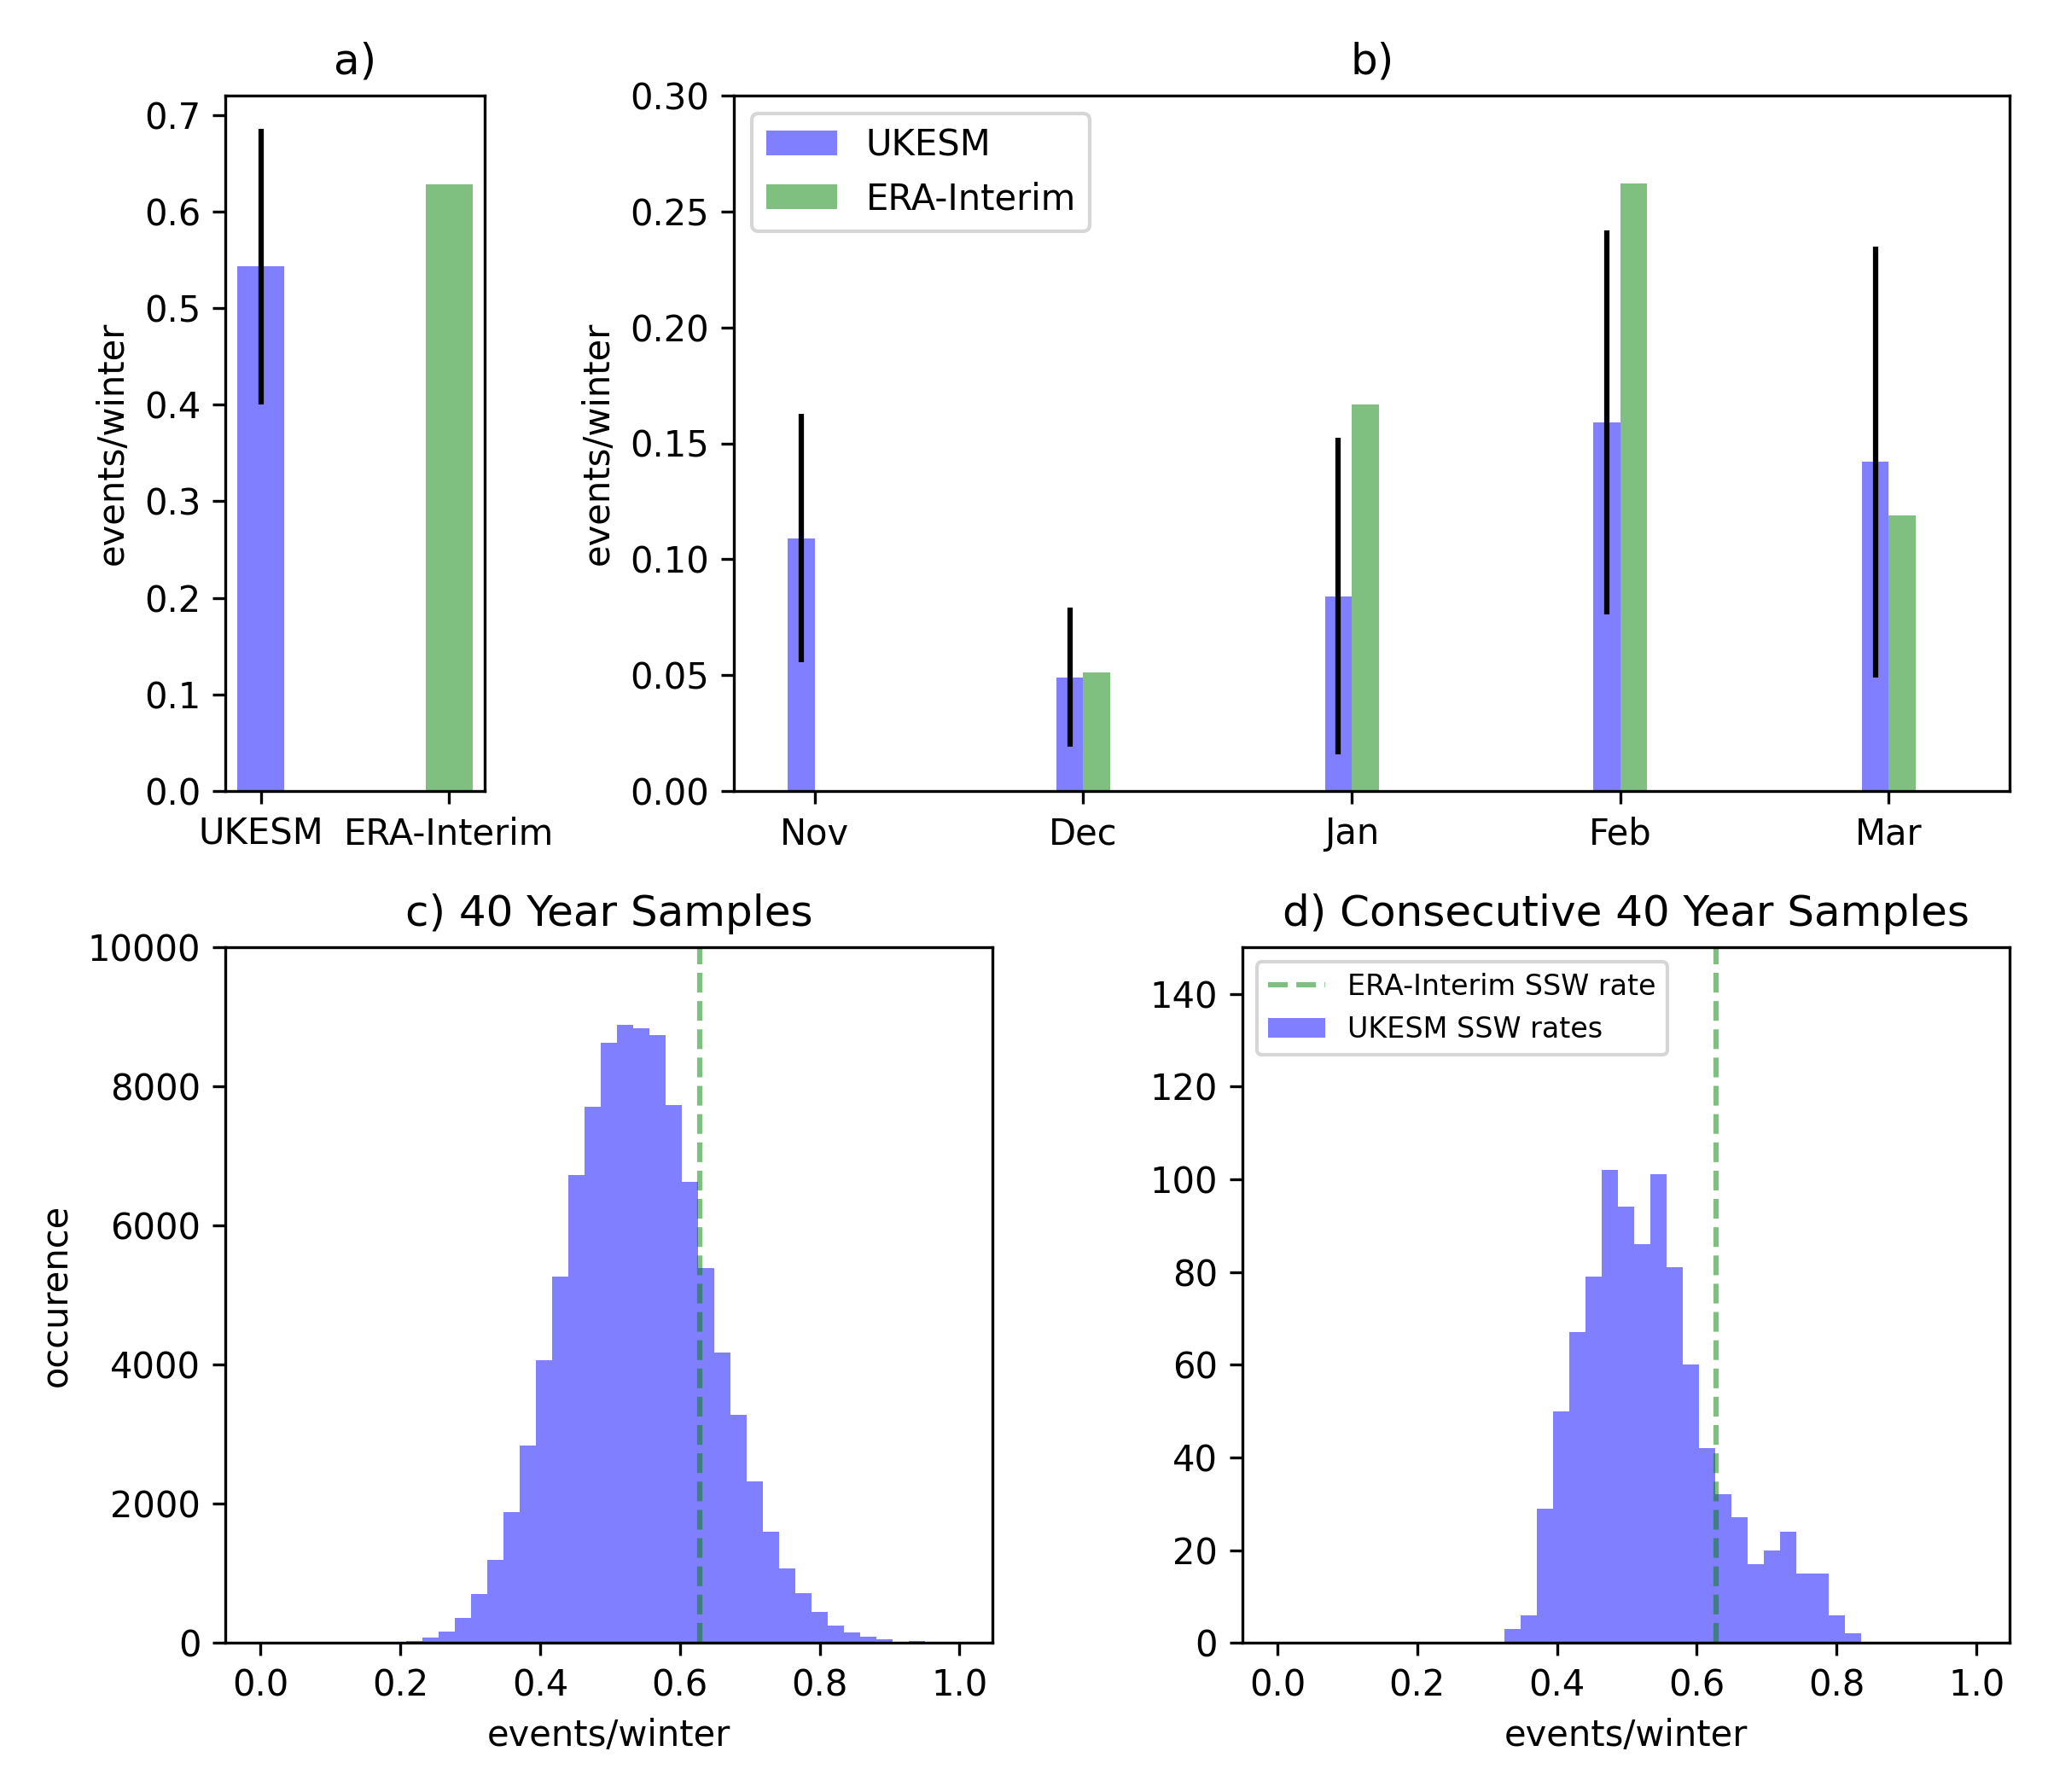
\includegraphics[width = 0.8\linewidth]{Figures/Figures-origins/SSW_hist_ERA_UKESM.png}
\caption[SSWs per NH winter season in the UKESM piControl and the ERA-Interim datasets.]{\textbf{a}: SSWs per NH winter season in the UKESM piControl and the ERA-Interim datasets. \textbf{b}: SSW rates separated by months. Error bars on a and b are derived using a bootstrap re-sampling method in which random selections of 40 years (the length of the reanalysis dataset) are chosen from the SSW data and the SSW rate recorded to build a PDF of events per season. 100000 such re-samples are carried out and the 95 and 5 percentile values are used as error bounds. This PDF is shown in blue bars in panel \textbf{c}. \textbf{d}: PDF of SSW rates in consecutive 40 year intervals of the UKESM simulation (blue bars). The SSW rate in ERA-Interim is indicated by the green dashed line in panels c and d.}
\label{fig:SSW_histogram}
\end{center}
\end{figure}

The model exhibits variability in SSW frequency comparable to observations, including both hiatus and consecutive SSW intervals. Figure \ref{fig:SSW_series_sample} shows a sample 40-yr interval of the polar vortex zonal wind strength and SSW occurrence from the UKESM simulation compared with a similar length from the ERA Interim reanalyses. An extended interval of mainly westerly anomalies indicating a strengthened vortex and lack of SSWs can be seen towards the end of the 40-yr interval, similar to the 1990s in ERA-Interim when only 2 SSW events were recorded in the decade. The simulation contains 8 such hiatus intervals with at least 10 consecutive years with no SSWs, the longest of which lasts 16 years. On the other hand, the simulation only contains 2 intervals in which 10 consecutive years exhibit at least 1 SSW. However, if the threshold interval width for identifying hiatus and consecutive-SSW intervals is shortened from 10 to 5 years, then 9 consecutive-SSW intervals and 25 hiatus intervals are found. These statistics indicate that UKESM is not only able to reproduce the mean state characteristics of SSW events but also decadal-scale variations in SSW rate, underlining its  suitability for this study. 

The second major mode of stratospheric variability is the QBO at equatorial latitudes which is present at all times of the year. Figure \ref{fig:equatorial_U_sample} shows the equatorial wind time-series from a sample 40-yr interval of the simulation compared with the ERA-Interim dataset. The mean period of the oscillation is longer than observed, at $\sim$38 months compared to $\sim$28 months in ERA-Interim \citep{kawataniRepresentation2016}. As a result the vertical shear zones descend less rapidly than observed. There is also a westerly bias at low levels where the QBO-E phase does not extend sufficiently deep into the lower stratosphere, which is a common bias in many models \citep{bushellEvaluation2020b}. The descending shear zones also appear more regular than observed but there is nevertheless some evidence of decadal-scale variations e.g. in the degree of stalling at 30\ hPa, although not as pronounced as in the observations.

\begin{figure}[h!]
\begin{center}
\noindent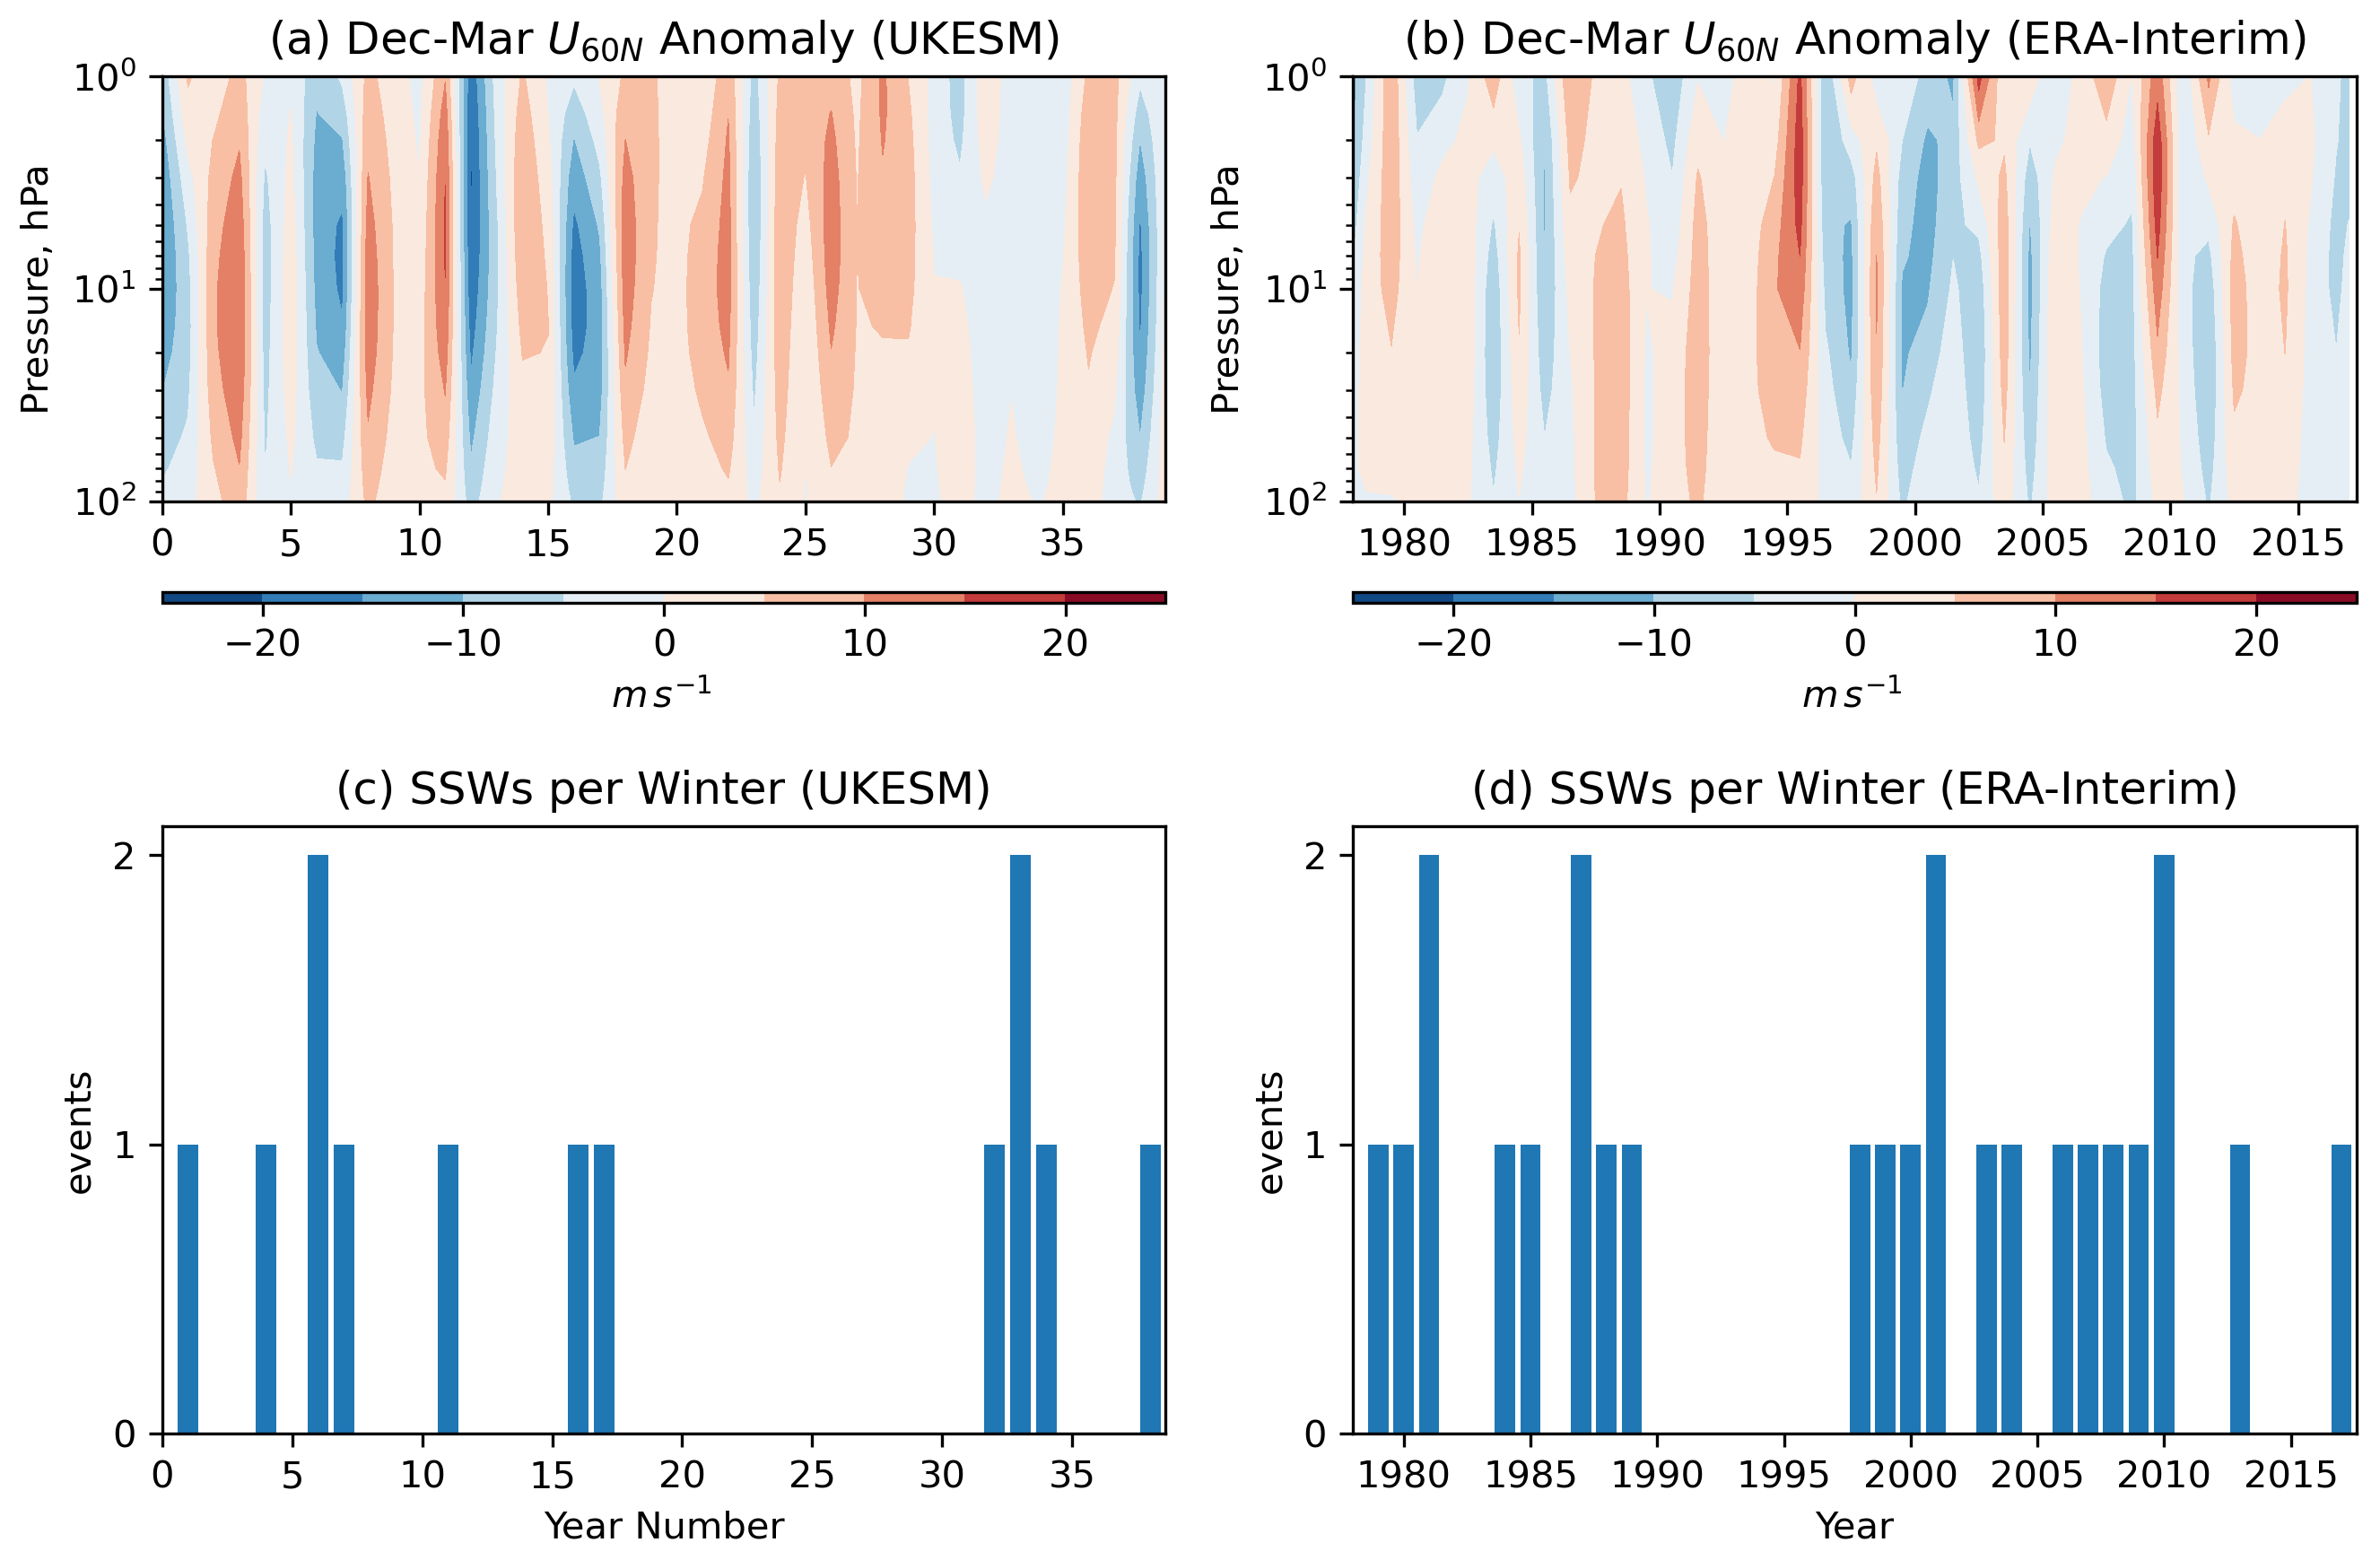
\includegraphics[width = \linewidth]{Figures/Figures-origins/SSW_series_ERA_UKESM.png}
\caption[Vortex ZMZW and SSW time series from UKESM pi-control and ERA-Interim]{\textbf{(a, b)}: Dec-Mar annual mean ZMZW anomaly from the climatological mean at 60$^\circ$\,N from a 40 year sample from the pre-industrial control simulation of UKESM \textbf{(a)} and the ERA-Interim dataset between 1979 and 2018 \textbf{(b)}. \textbf{(c, d)}: Time series of SSWs recorded per winter season in the same datasets.}
\label{fig:SSW_series_sample}
\end{center}
\end{figure}

%---------------------------------------------------------------

\begin{figure}[h!]
\begin{center}
\noindent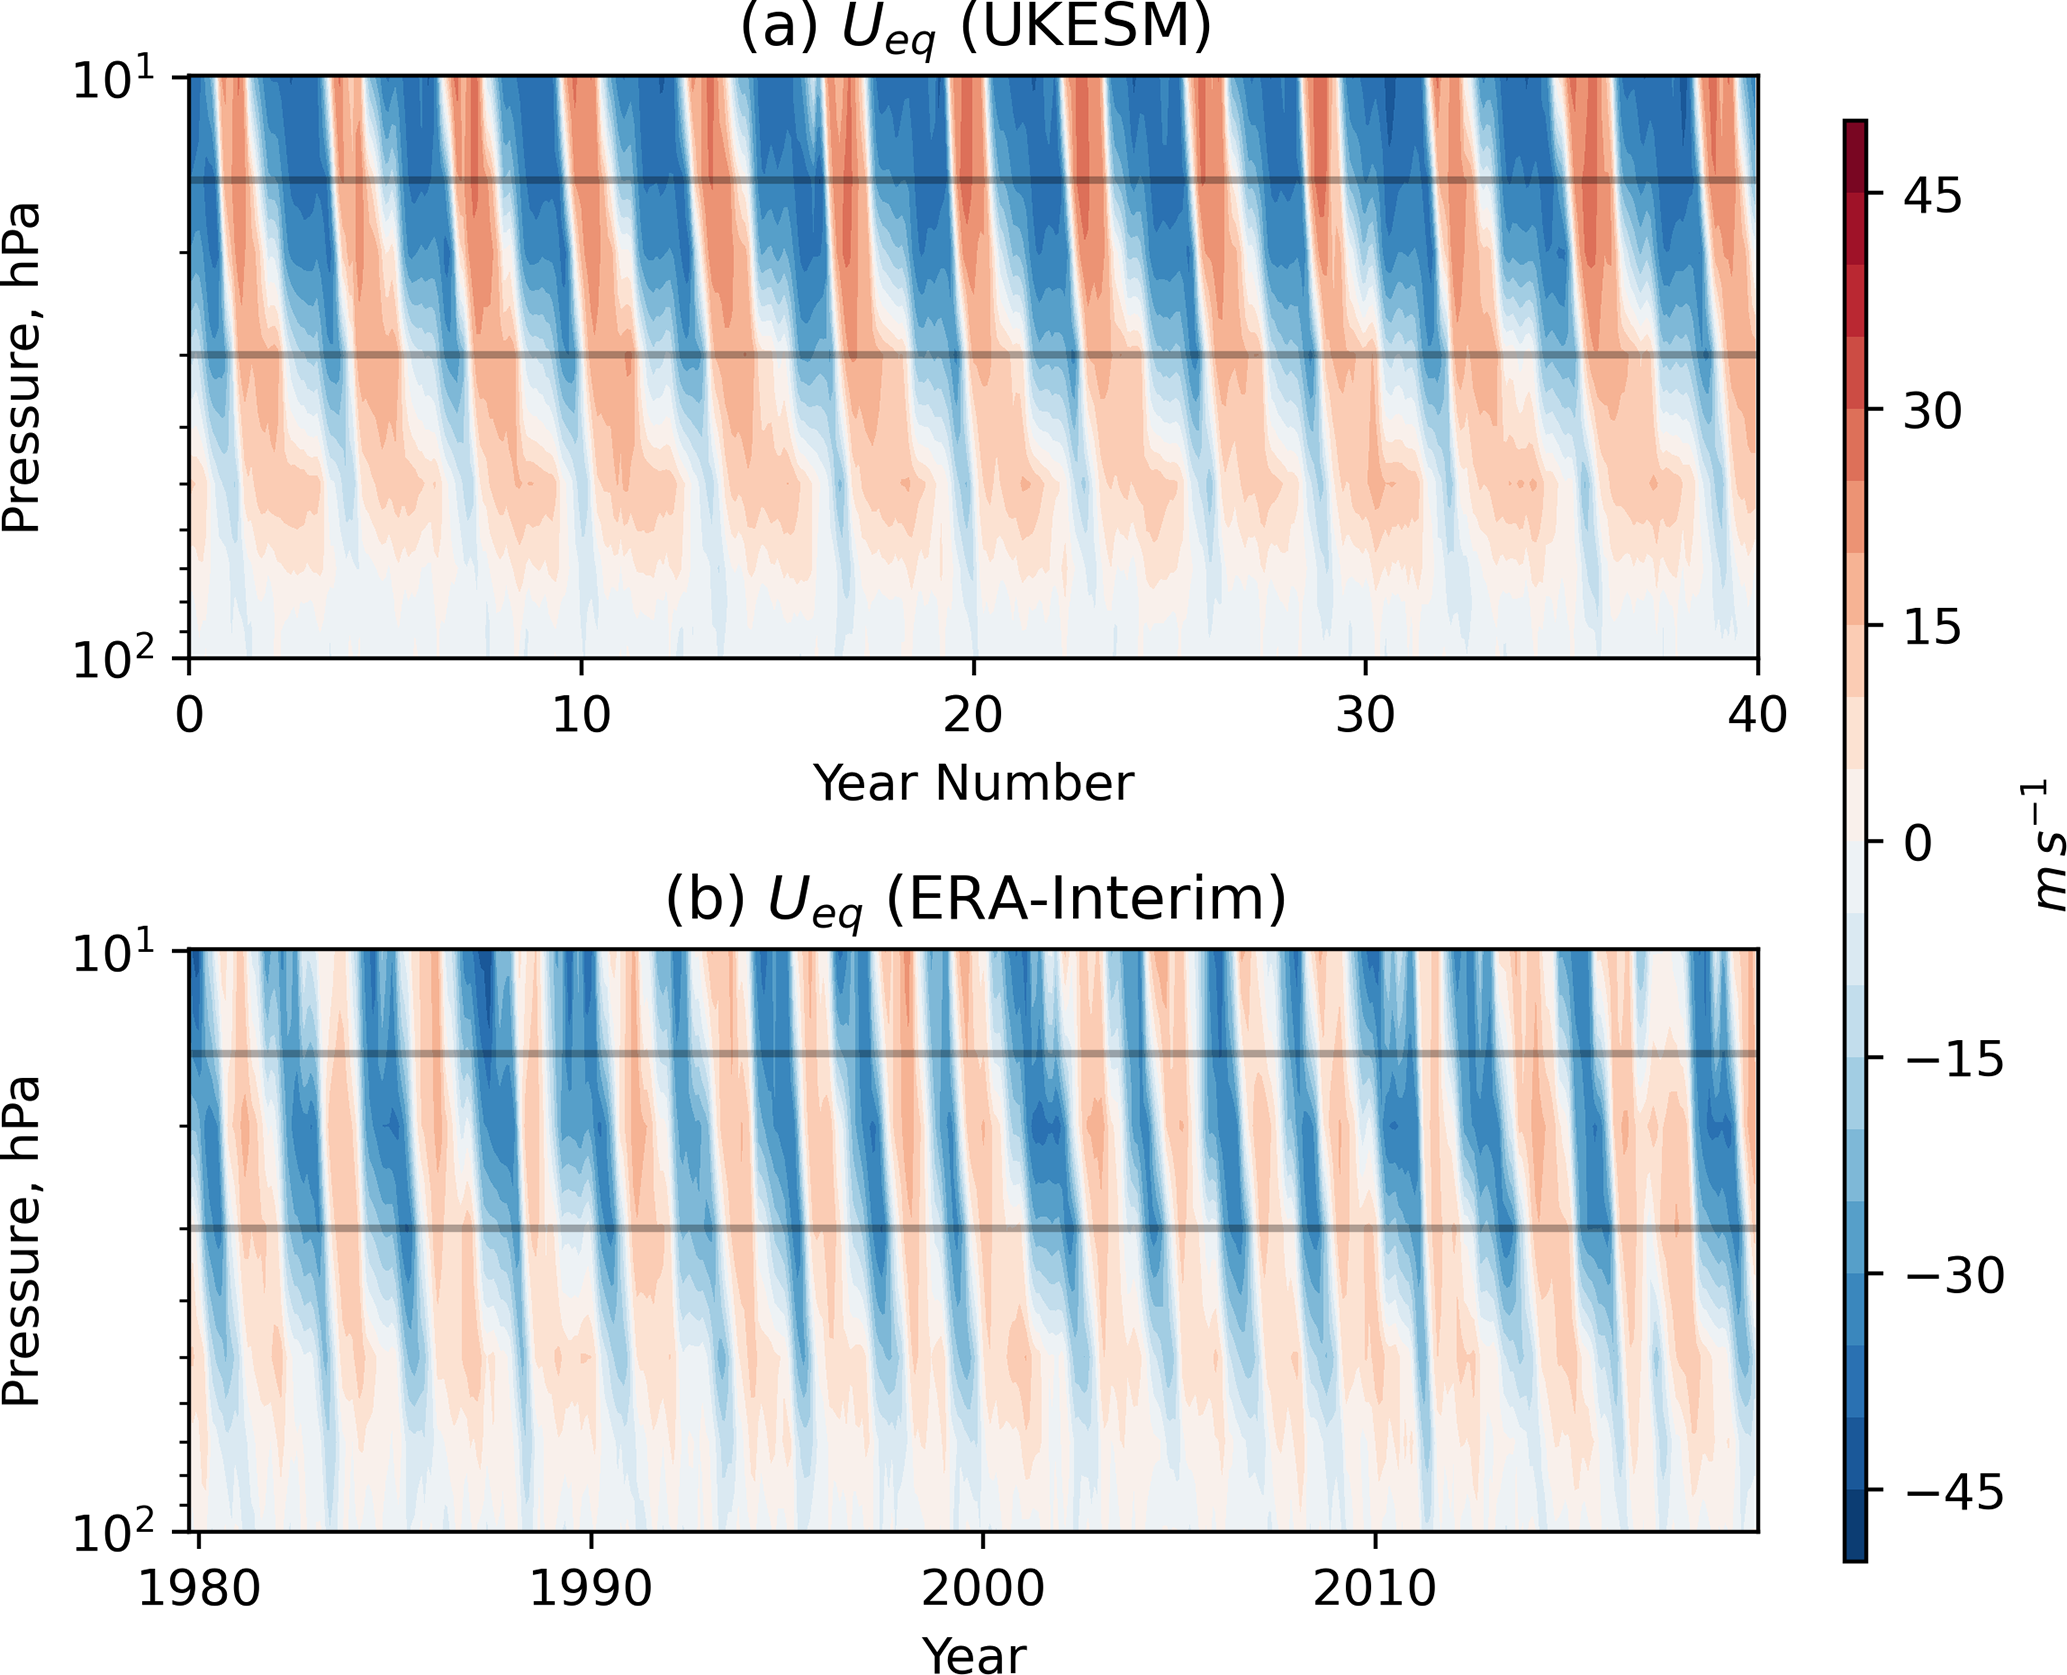
\includegraphics[width = 0.8\linewidth]{Figures/Figures-origins/equatorial_U_UKESM_ERA.png}
\caption[Time-height profiles for equatorial ZMZW from the UKESM pi-control and ERA-Interim.] {ZMZW averaged between 5$^{\circ}$\,S--5$^{\circ}$\,N latitude from from a 40 year sample of the pre-industrial control simulation of UKESM \textbf{(a)} and the ERA-Interim dataset between 1979 and 2018 \textbf{(b)}. Horizontal lines mark the 15\,hPa and 30\,hPa levels between which the deep QBO metric employed by \cite{andrewsObserved2019d} is defined.}
\label{fig:equatorial_U_sample}
\end{center}
\end{figure}


%---------------------------------------------------------------

There is evidence of coupling between the two major modes of stratospheric variability in the model, giving rise to a Holton-Tan relationship \citep{ansteyHighlatitude2014b}. Figure \ref{fig:holton_tan_comp} shows height-latitude cross-sections of NH winter zonal wind differences between QBO E-W composites defined at various equatorial levels. The familiar pancake structure of alternating easterly / westerly differences is present at equatorial latitudes, indicative of the QBO phase but there is also a response at high latitudes. In good agreement with observations the largest high latitude response amplitude is seen when  the QBO is defined at 50hPa, with anomalously weaker polar vortex strength in QBO-E than in QBO-W years. Higher levels (15\,hPa and 20\,hPa) show little significant QBO-vortex coupling. For comparison we also show in figure \ref{fig:holton_tan_comp} the composite different response for QBO composites selected on the basis of the average QBO winds over a greater depth of the equatorial atmosphere (15-30 hPa and 20-50 hPa). We note that while this QBO definition will select some of the same years as in the separate single-level composite definitions, it is specifically designed to identify only QBO  phases that have extended vertical coherence, following \citep{graySurface2018b} and \cite{andrewsObserved2019d}, so the resulting composite differences in figure \ref{fig:holton_tan_comp} will not necessarily be an average of the corresponding single-level differences. Interestingly, the 15--30 hPa deep-QBO selects years that exhibit not only a weaker polar vortex in QBO-E but also a weaker sub-tropical tropospheric jet (see 200 hPa, 30$\degree$-40$\degree$N). This results in a more coherent response in the mid-latitude troposphere and at the surface, in excellent agreement with the results of \cite{graySurface2018b} and \cite{andrewsObserved2019d}. 

%---------------------------------------------------------------

\begin{figure}[h!]
\begin{center}
\noindent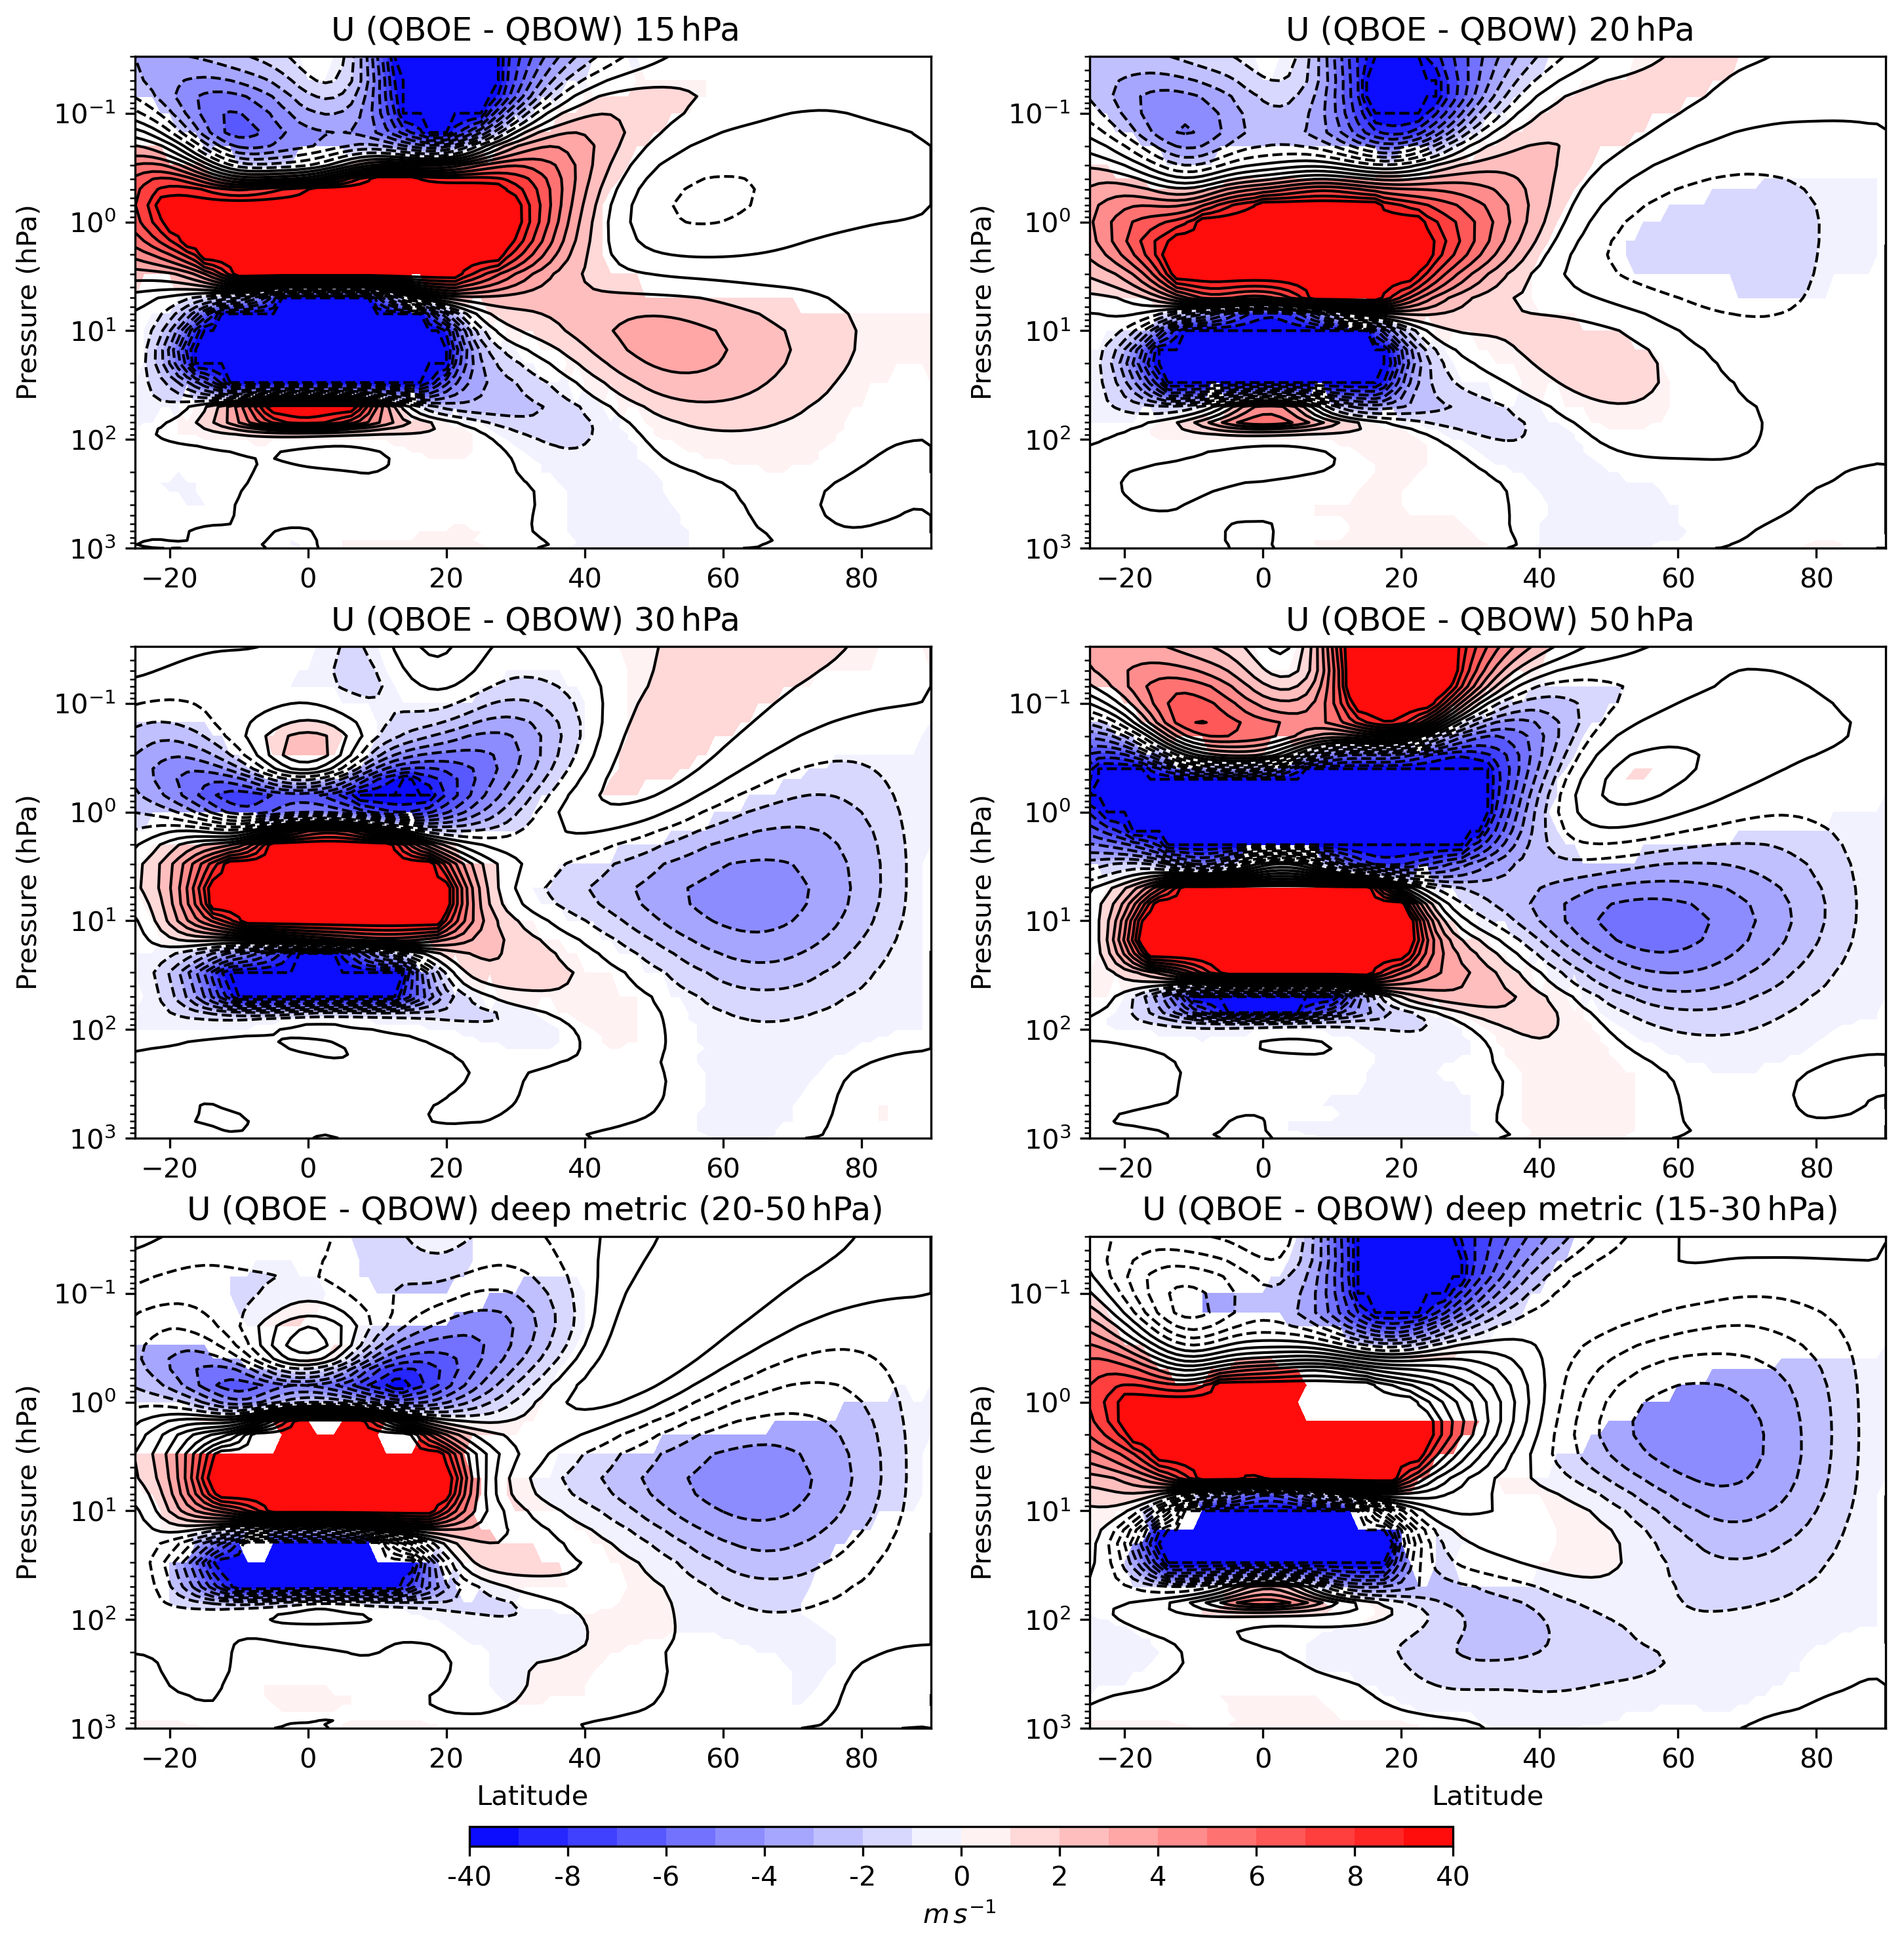
\includegraphics[width = 0.85\linewidth]{Figures/Figures-origins/holton_tan_composites.png}
\caption[ZMZW composite differences between QBO phases in the UKESM pi-control.]{Dec-Mar ZMZW composite differences between QBO East and QBO West phases evaluated in Sep-Oct at individual levels as well as using the deep QBO metric. The phase of the QBO is defined any Sep-Nov equatorial ($5^{\circ}$\ S--$5^{\circ}\ $N average) ZMZW that exceeds a magnitude of 5\ m\,s$^{-1}$. Coloured shading indicates differences significant above the 95\% confidence level under a 2 tail student’s t-test.}
\label{fig:holton_tan_comp}
\end{center}
\end{figure}

The presence of the Holton-Tan relationship is also seen in the modelled frequency of SSWs (figures 5). Significantly higher rates are observed in QBO-E winters than QBO-W. Also notable is the asymmetry in abundance of QBO-E and QBO-W winters - nearly twice as many QBO-E winters are observed compared to QBO-W under all phase definitions (figure \ref{fig:SSW_hist_QBO_phase}, legends). This suggests an element of phase locking between the QBO and the seasonal cycle possibly associated with seasonally variations in the strength of mean equatorial upwelling or mid-latitude planetary wave forcing in winter \citep{pascoeQuasibiennial2005b, gruzdevTwo2000b, rajendranSynchronisation2016b} resulting in QBO phase transitions that occur preferentially in certain months. 

\begin{figure}[h!]
\begin{center}
\noindent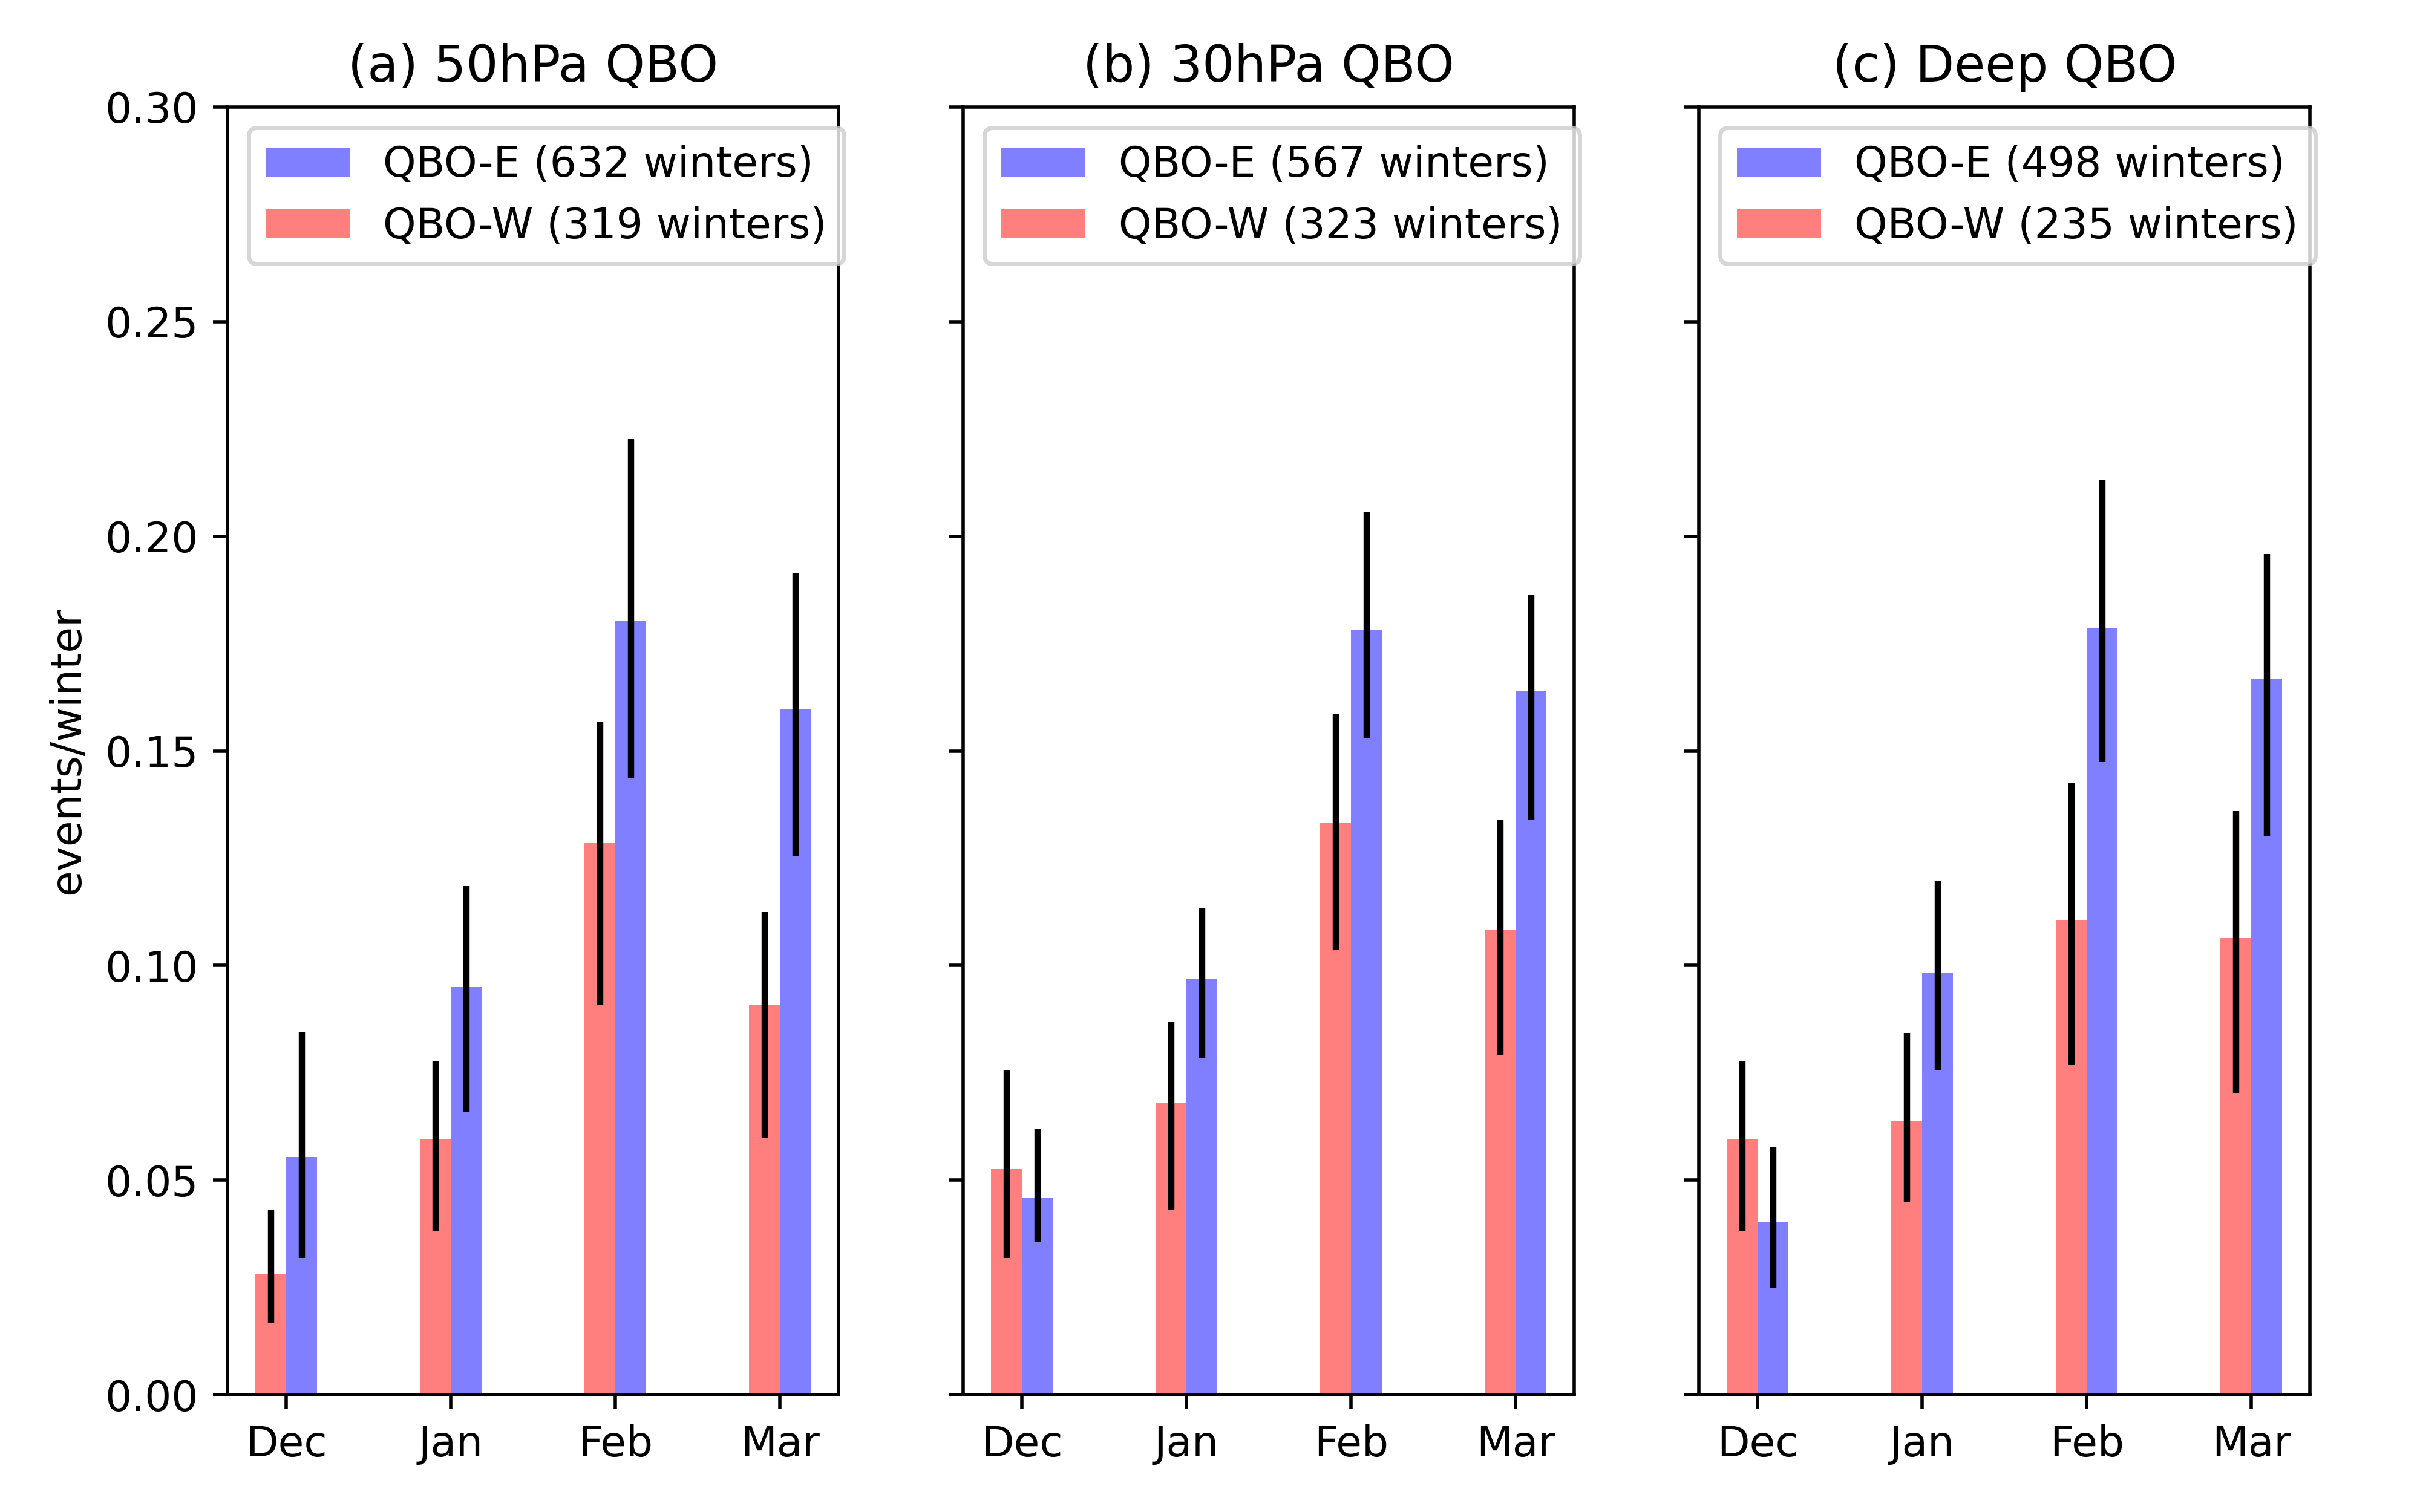
\includegraphics[width = 0.9\linewidth]{Figures/Figures-origins/SSW_histograms_QBOphases.png}
\caption[Histogram of SSWs per winter in different QBO phases.]{SSWs per winter season for years exhibiting QBO-E and QBO-W conditions in early winter (Sep-Nov) defined on different pressure levels (a,b) as well as using the deep metric (c), the vertical mean between 15 and 30\,hPa defined in \cite{andrewsObserved2019d}. The QBO phase is defined as any Sep-Nov equatorial ($5^{\circ}$\ S--$5^{\circ}\ $N average) ZMZW that exceeds a magnitude of 5\ m\,s$^{-1}$. Error bars on all plots are derived using the same bootstrapping method outlined in figure \ref{fig:SSW_histogram}}
\label{fig:SSW_hist_QBO_phase}
\end{center}
\end{figure}

There is also evidence of in-season coupling between the vortex and phases of ENSO as well as the AL. Composites of ZMZW under different Ni\~{n}o3.4 conditions (figure \ref{fig:ZMZW_comp_ENSO_AL}a, b) shows a response from vortex winds to the 2 types of anomalous ENSO behaviour. The vortex appears significantly stronger under La Ni\~{n}a conditions and weaker under El Ni\~{n}o, a result which is consistent with numerous studies from both observations and other models (see section \ref{sec:external_influence_SSTs}). As is noted in \cite{polvaniDistinguishing2017b}, the vortex response to ENSO in the model appears more linear than those generally found in observation based studies; the magnitude of responses to each phase is similar. In contrast, the vortex response to different signs of the AL (figure \ref{fig:ZMZW_comp_ENSO_AL}c, d) index is highly asymmetric. The vortex is considerably weakened under anomalously negative AL values (corresponding to a more intense Aleutian Low) while the positive AL phase only leads to a marginal strengthening in vortex winds. This may me due to the proposed mechanism by which the AL influences the vortex, via alteration of planetary wave propagation into the stratosphere. This provides modulation of the weakening mechanism of the vortex under negative AL but not a strengthening under positive - simply an absence of wave fluxes. Nevertheless, these AL composites are consistent with the findings of studies outlined in \ref{sec:external_influence_AL} which report a weakened vortex under negative AL conditions. Both sets of composites indicate that the model is able to reproduce expected in-season vortex responses from these key modes of surface variability, further suggesting its suitability for an analysis of external influence on the vortex from these modes on multi-decadal timescales. 

\begin{figure}[h!]
\begin{center}
\noindent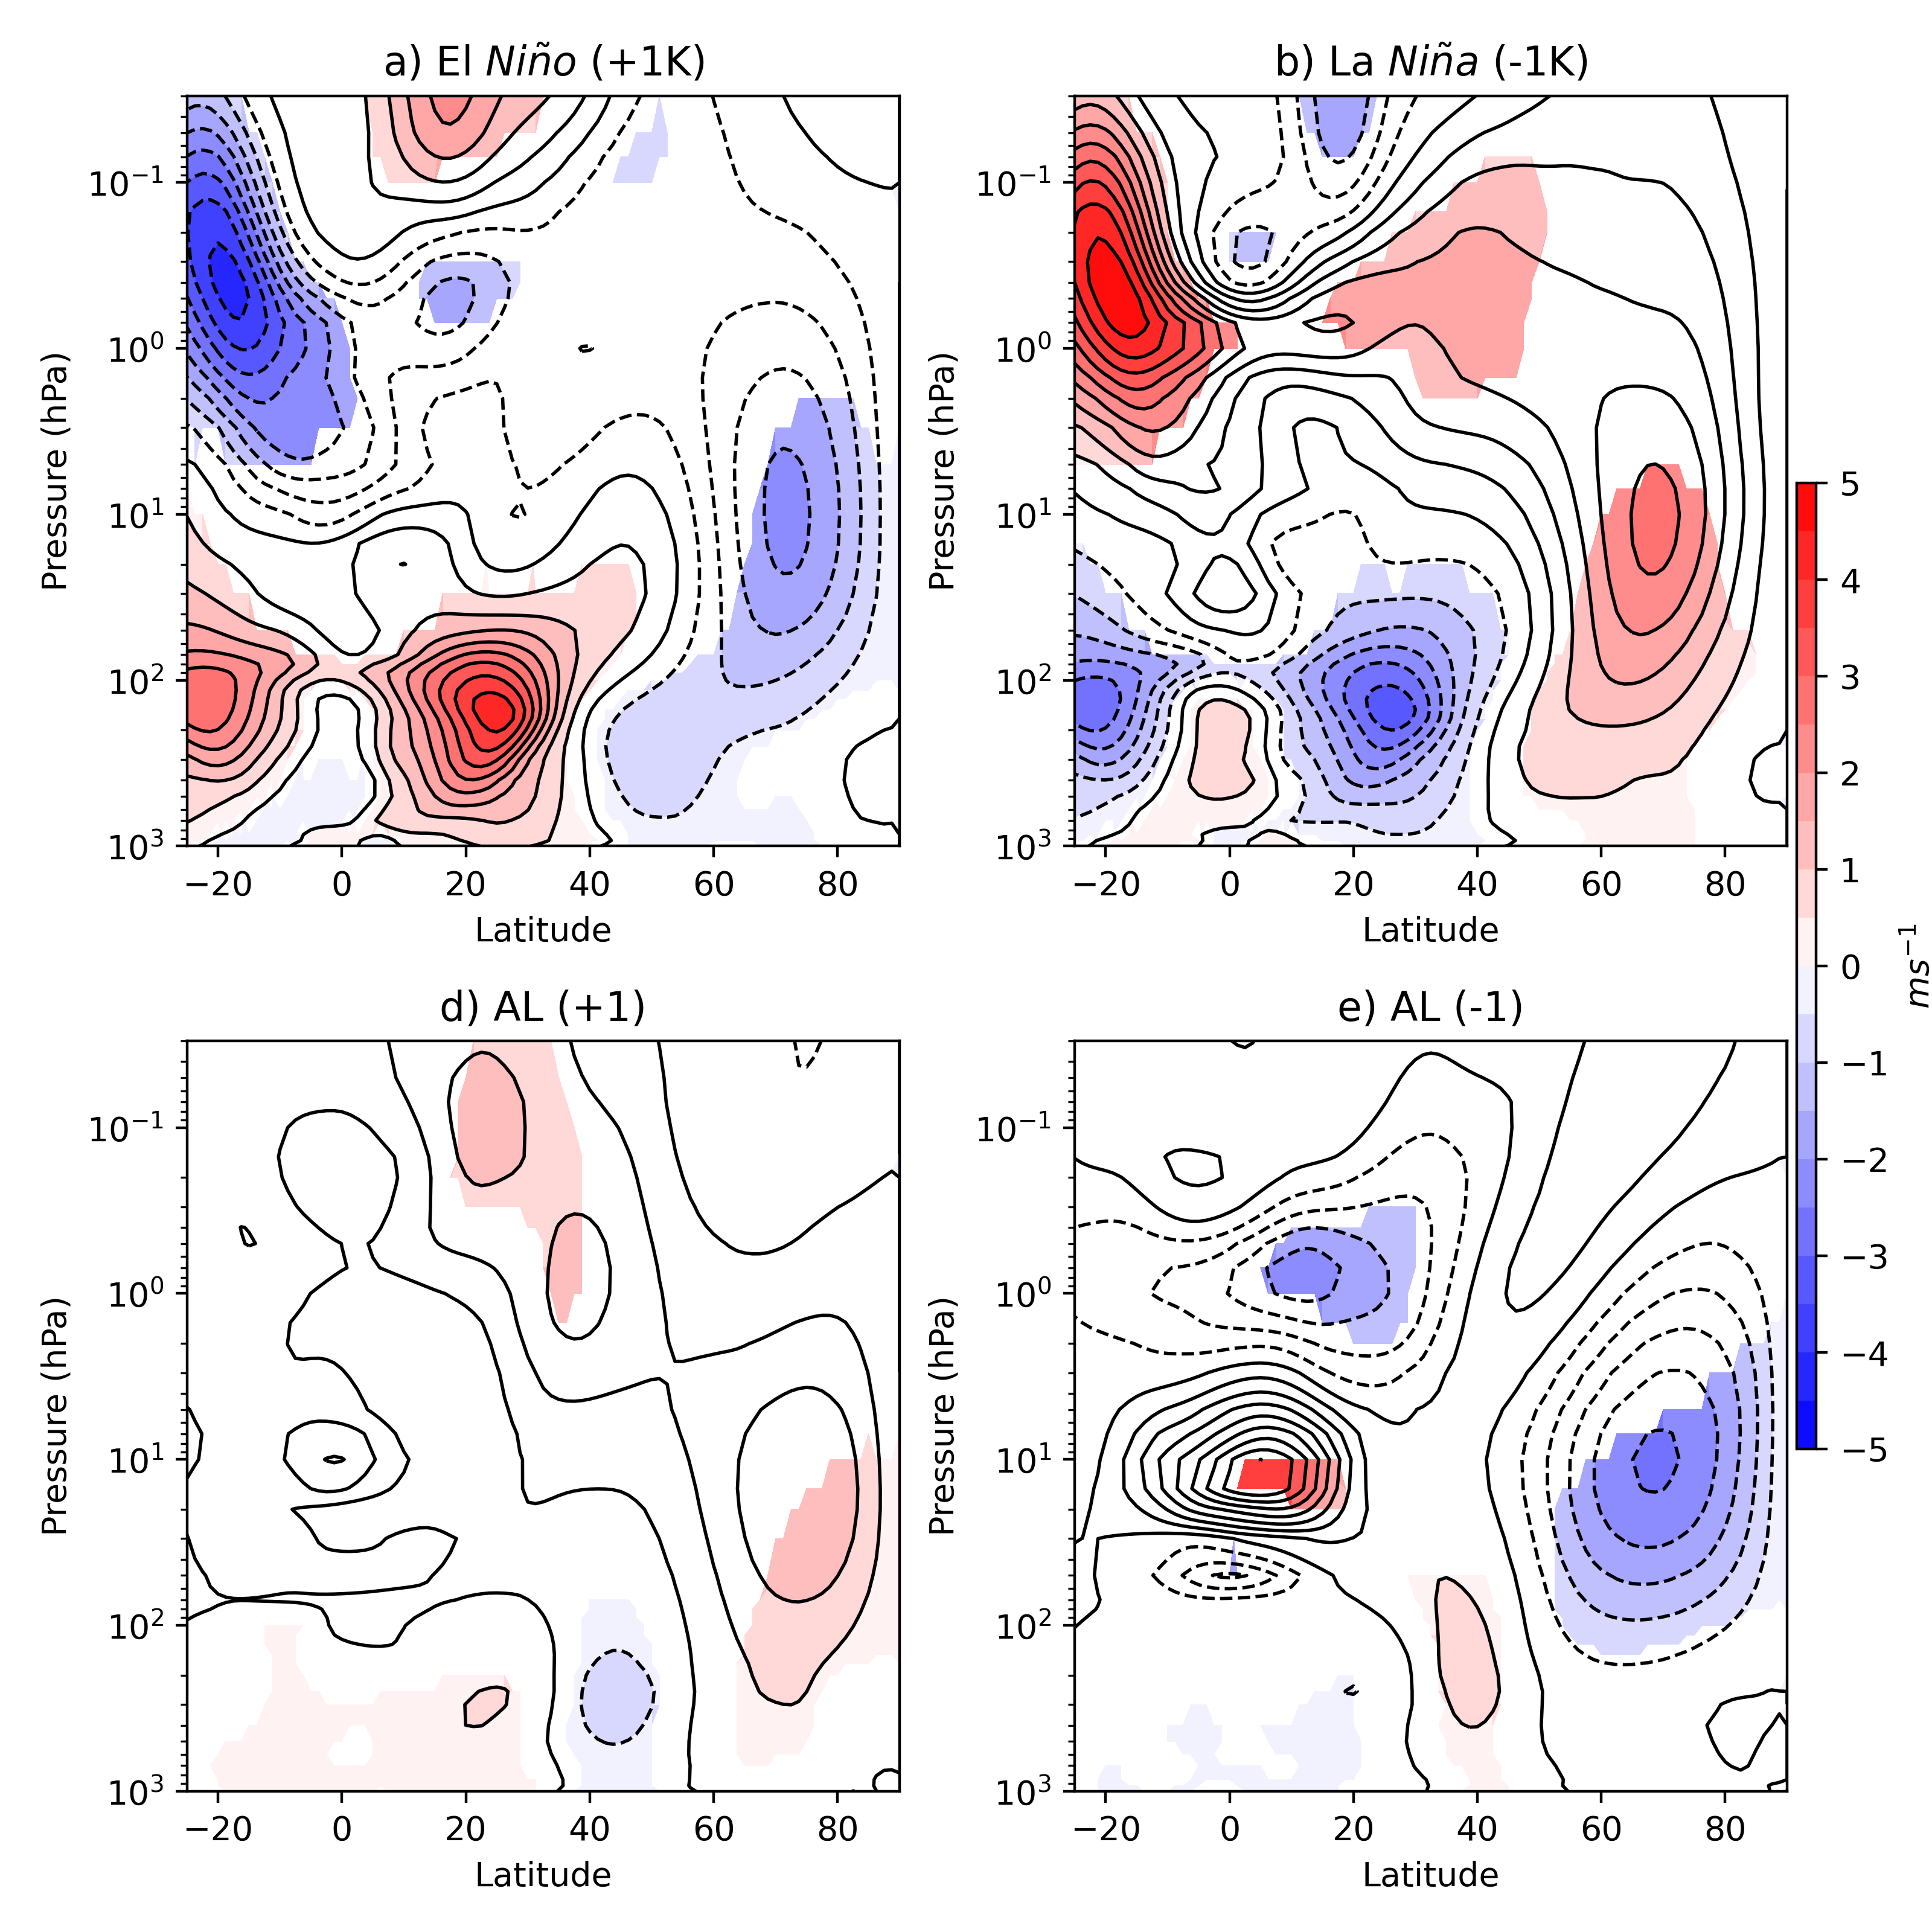
\includegraphics[width = 0.75\linewidth]{Figures/Figures-origins/ZMZW_comps_ENSO_AL.png}
\caption[Dec-Mar ZMZW anomaly composites for different phases of ENSO and the AL]{Dec-Mar ZMZW anomaly composites for positive (El Ni\~{n}o) and negative (La Ni\~{n}a) phases of the Ni\~{n}o3.4 index evaluated in Sep-Nov (a, b) and the Aleutian low index evaluated in Dec-Feb (c, d). The phase of Ni\~{n}o3.4 is defined as an SST anomaly of greater magnitude than 1K and the AL phase as an index value derived using the principal component based definition of greater magnitude than 1. Coloured shading indicates anomalies significant above the 95\% confidence level under a 2-tailed student’s t-test.}
\label{fig:ZMZW_comp_ENSO_AL}
\end{center}
\end{figure}



\section{Regression Analysis}
We next employ a multi-linear regression analysis to measure the relative contributions to the time-series of SSWs per year (as in figure \ref{fig:SSW_series_sample}) from the QBO, ENSO and the Aleutian low. The results from this analysis are summarised in table 1.  Sensitivity experiments were performed to identify the optimum averaging lagged response by the vortex to each index: the deep 15-30 hPa QBO index and Ni\~{n}o3.4 indices were both defined using early winter (Sep-Nov) averages while the AL index was defined using Dec-Mar averages. The coefficients are all significant to the 95\% level but are relatively small and the $R^2$ score is only 0.047 indicating these variables account for only a small portion of the variability in the SSW timeseries. While results from this multi-linear regression analysis are easy to interpret, the approach does not directly tackle the problem posed in this study, that of multi-decadal variability in SSWs and its origins, for two main reasons. Firstly, regression analysis assumes stationarity i.e. it provides a measure of stationary contributions to variability and will only highlight signals that are relatively persistent for the whole simulation. Secondly, it  analyses variability in the time series at all timescales simultaneously, so that the results are dominated by the timescales with larger amplitude variations.  This means that the results in table 1 are most likely dominated by the shorter (inter-annual) timescales and any small amplitude variations at longer timescales will not be revealed. The latter can be addressed to some extent by smoothing or filtering the time-series, as discussed in the next section, but this requires prior knowledge of which frequencies are of interest. Furthermore, co-variability in predictor indices of a regression model may lead to spurious coefficients. This may be an issue here as \cite{raoModulation2019d} note correlations between ENSO and the AL. The variance inflation factor is a measure of the degree to which each regression coefficient is altered by predictor co-variations. the VIF for each predictor is greater than 1 indicating a moderate degree of co-variation with other predictors \citep{akinwandeVariance2015b} which may further hamper the efficacy of this regression method. An alternative and superior approach to this problem employs wavelet analysis, described more fully in the next section, which successively examines different frequency intervals to identify the presence of signals thus avoiding dominance by one particular frequency, and also measures the time evolution of the signal so that non-stationary signals can also be identified. 

\begin{table}[h!]
\centering
\begin{tabular}{|p{3cm}||p{3cm}|p{3cm}|}
 \hline
 \multicolumn{3}{|c|}{SSW regression}\\
 \hline
 Regression Variable& Coefficient& p value\\
 \hline
 Ni\~{n}o3.4  & 0.1625$^+_-$0.035& 0.0002\\
 AL  &   -0.0927$^+_-$0.04  & 0.048\\
 deep QBO  & -0.1993$^+_-$0.03&0.0001\\
 \hline
 \end{tabular}
\begin{center}
\caption{Summary of results from regression analysis of SSWs per NH winter time series.}
\label{table:regression_SSW}
\end{center}
\end{table}

%---------------------------------------------------------------

\section{Long-term Variability of the Polar Vortex}
A more comprehensive assessment of the long-term variability of SSWs can be made using a wavelet power spectrum approach outlined in section \ref{sec:Wavelet_Analysis}. We count the number of SSWs in each winter season (Dec-Mar) and calculate the corresponding wavelet power spectrum, shown in figure \ref{fig:SSW_series_wavelet}. As described above, the analysis highlights the presence of power in the signal as a function of frequency (period in years, along the y-axis) and as a function of time (year of simulation along the x-axis). As expected, there is an intermittent but relatively persistent signal with period around 2-4 years throughout the simulation, corresponding to the period of the QBO which supports the presence of a Holton-Tan relationship between the QBO and the polar vortex in the model. The so-called 'global power spectrum' (i.e. the time average of the wavelet spectrum) shown on the right of figure \ref{fig:SSW_series_wavelet} shows that the signal is on the boundary of the 95\% statistical significance. Other signals at periods near 20-30 years are similarly intermittent and manifest as a peak in the time-averaged spectrum that is also near the 95\% significance boundary. There is also a feature at periods between $\sim$60-90 years in the interval between 400-800 yrs. This feature shows statistical significance (based on comparisons between power in the spectrum and that of an AR1 process with the same autocorrelation structure as the series being analysed) for around 300 years of the 1000-yr simulation but does not cross the significance threshold for the time-averaged spectra. There is a possible limitation of this wavelet methodology due to the discrete nature of the time series being analysed (time points take values 0/1/2). The Morlet wavelet is a continuous function and, as a result, convolution with a highly discretised series may alias features on the resulting wavelet spectra. This limitation must be considered when drawing conclusions from the wavelet spectra and is discussed further below.

\begin{figure}[h!]
\begin{center}
\noindent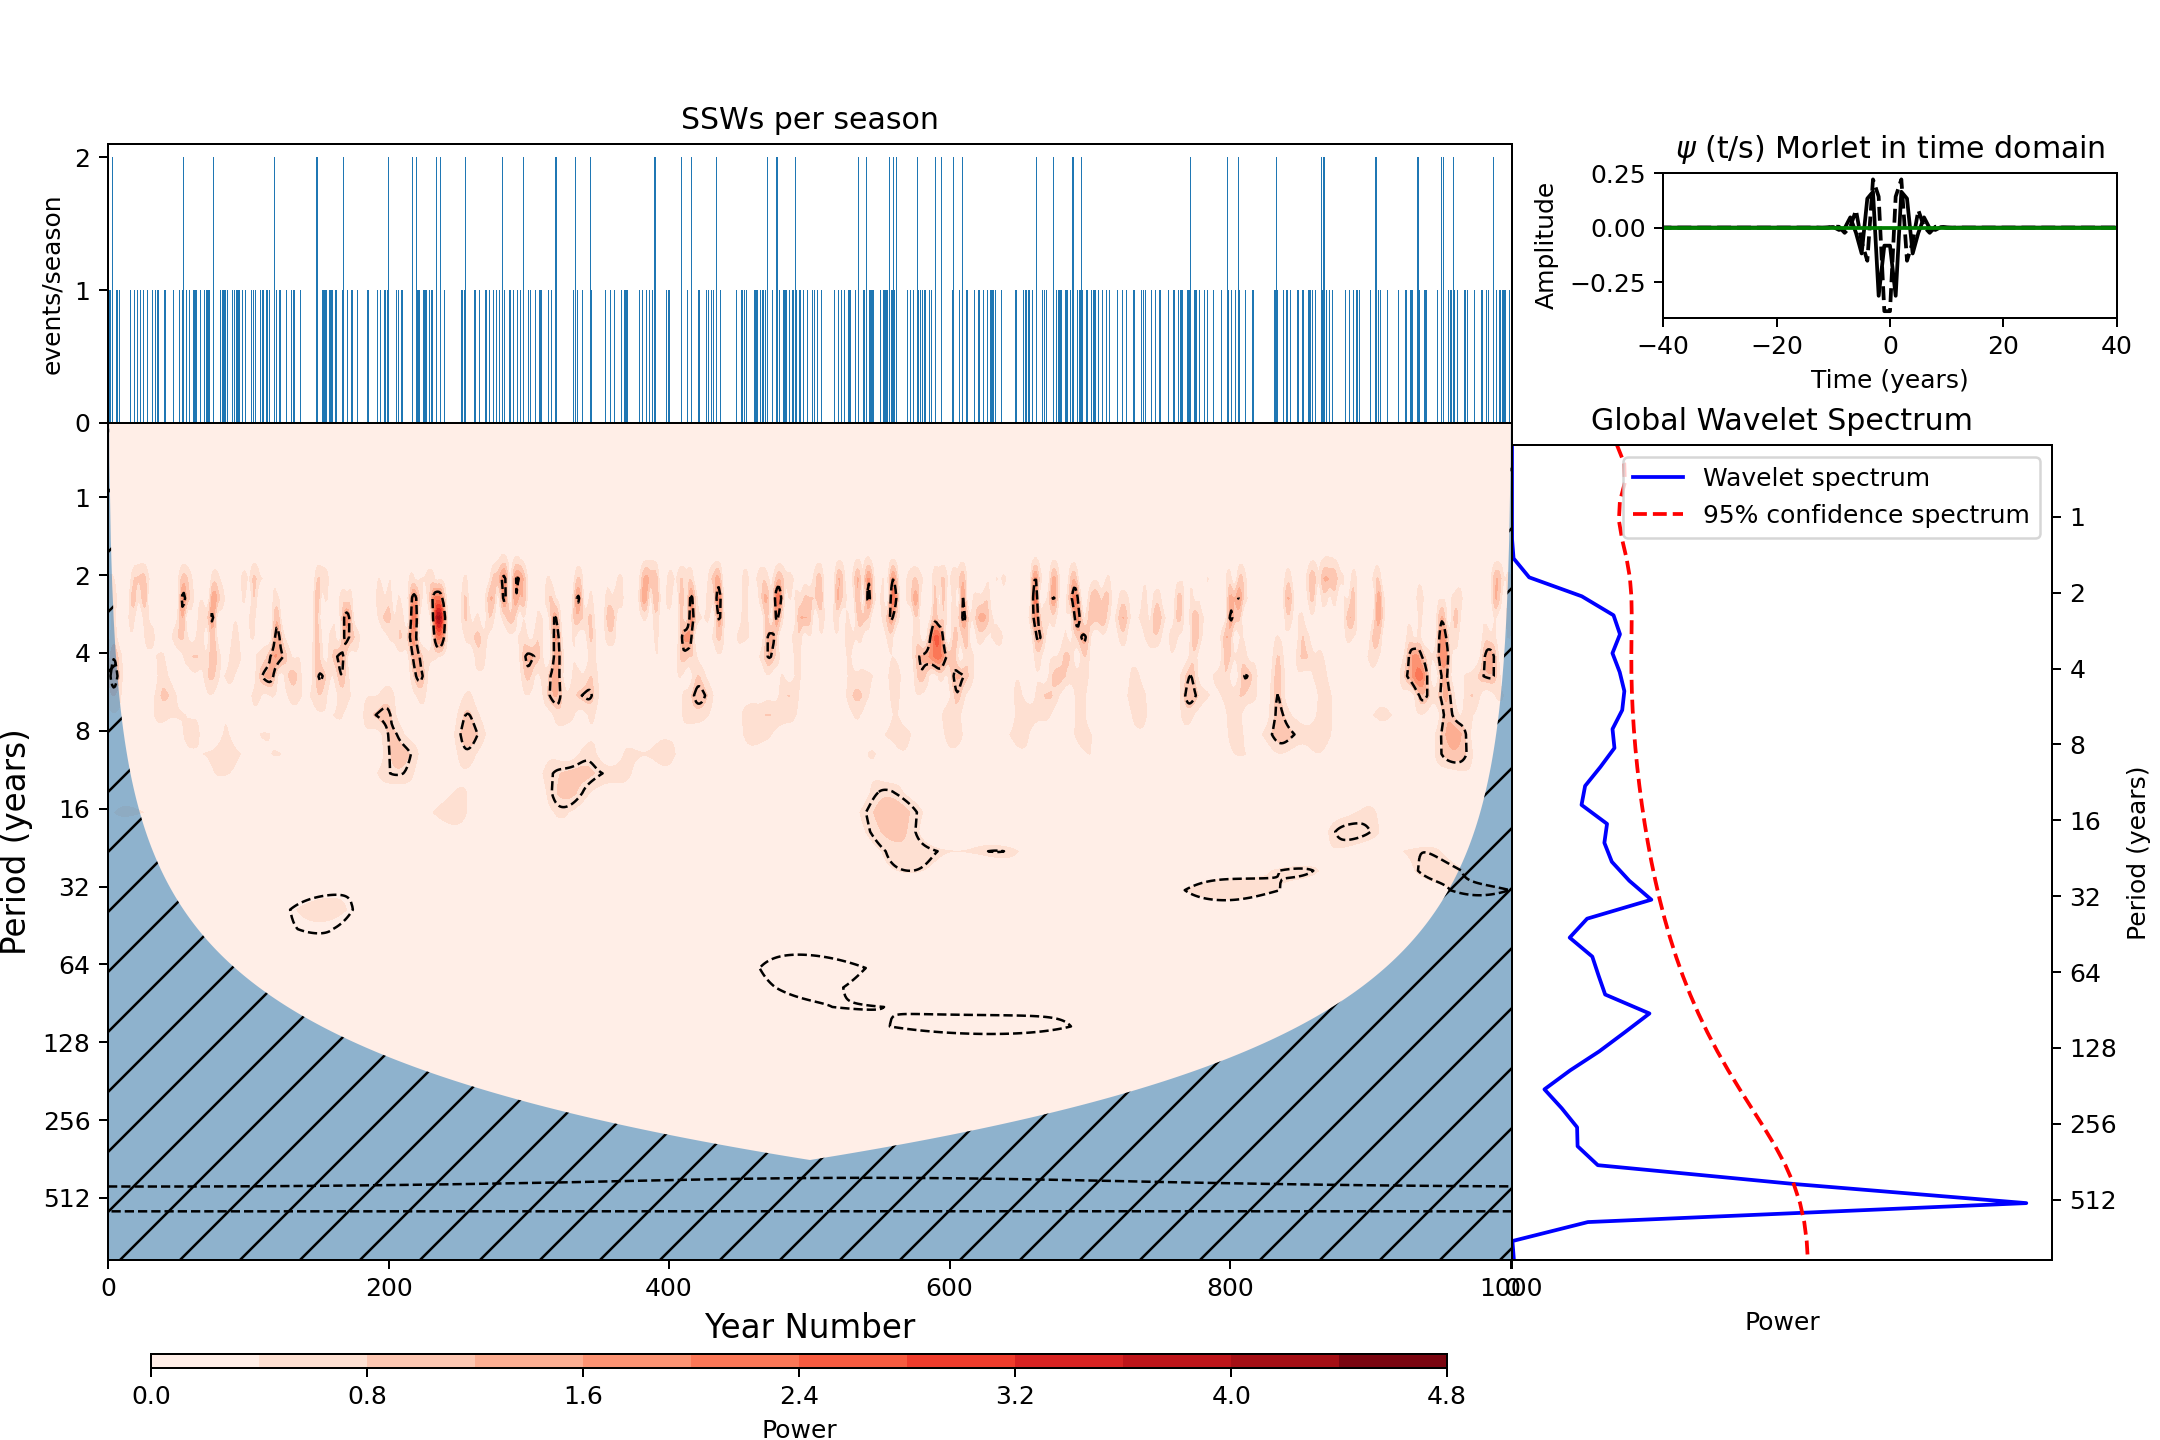
\includegraphics[width = 0.8\linewidth]{Figures/Figures-origins/SSW_wavelet.png}
\caption[Wavelet power spectrum for the SSW per NH winter time series]{\textbf{Top left}: SSW events per Dec-Mar season in UKESM \textbf{Bottom left}: Wavelet power spectrum of time series in top left. Hatching represents area outside the cone of influence in which edge effects are significant and power should not be considered. Yellow contours represent the 95\% confidence level assuming mean background AR1 red noise. \textbf{Top Right}: Morlet wavelet used for the wavelet transform in the time domain. \textbf{Bottom right:} Global power spectrum, the wavelet power averaged over the whole simulation (blue line), and global 95\% confidence spectrum (red dashed line).}
\label{fig:SSW_series_wavelet}
\end{center}
\end{figure}

%---------------------------------------------------------------

The focus of this study is on the longer-term time variations to understand the source of variability characterised by hiatus intervals (no SSWs over an extended period) and consecutive-event intervals (at least one SSW every year for an extended period). We therefore apply low-pass filtering to the time series of SSWs per season using a 5-year rolling window and examine the spectral characteristics of this smoothed series (which we refer to henceforth as $SSW_{5yr}$). This averaging is similar to the standard practice of smoothing daily data to remove the noise associated with daily weather variations, thus isolating longer seasonal timescales. It also decreases the impact of the time series discretisation and therefore reduces the chance of introducing spurious spectral features on the wavelet power spectrum which could be otherwise encountered when analysing the un-smoothed time series.  

\begin{figure}[h!]
\begin{center}
\noindent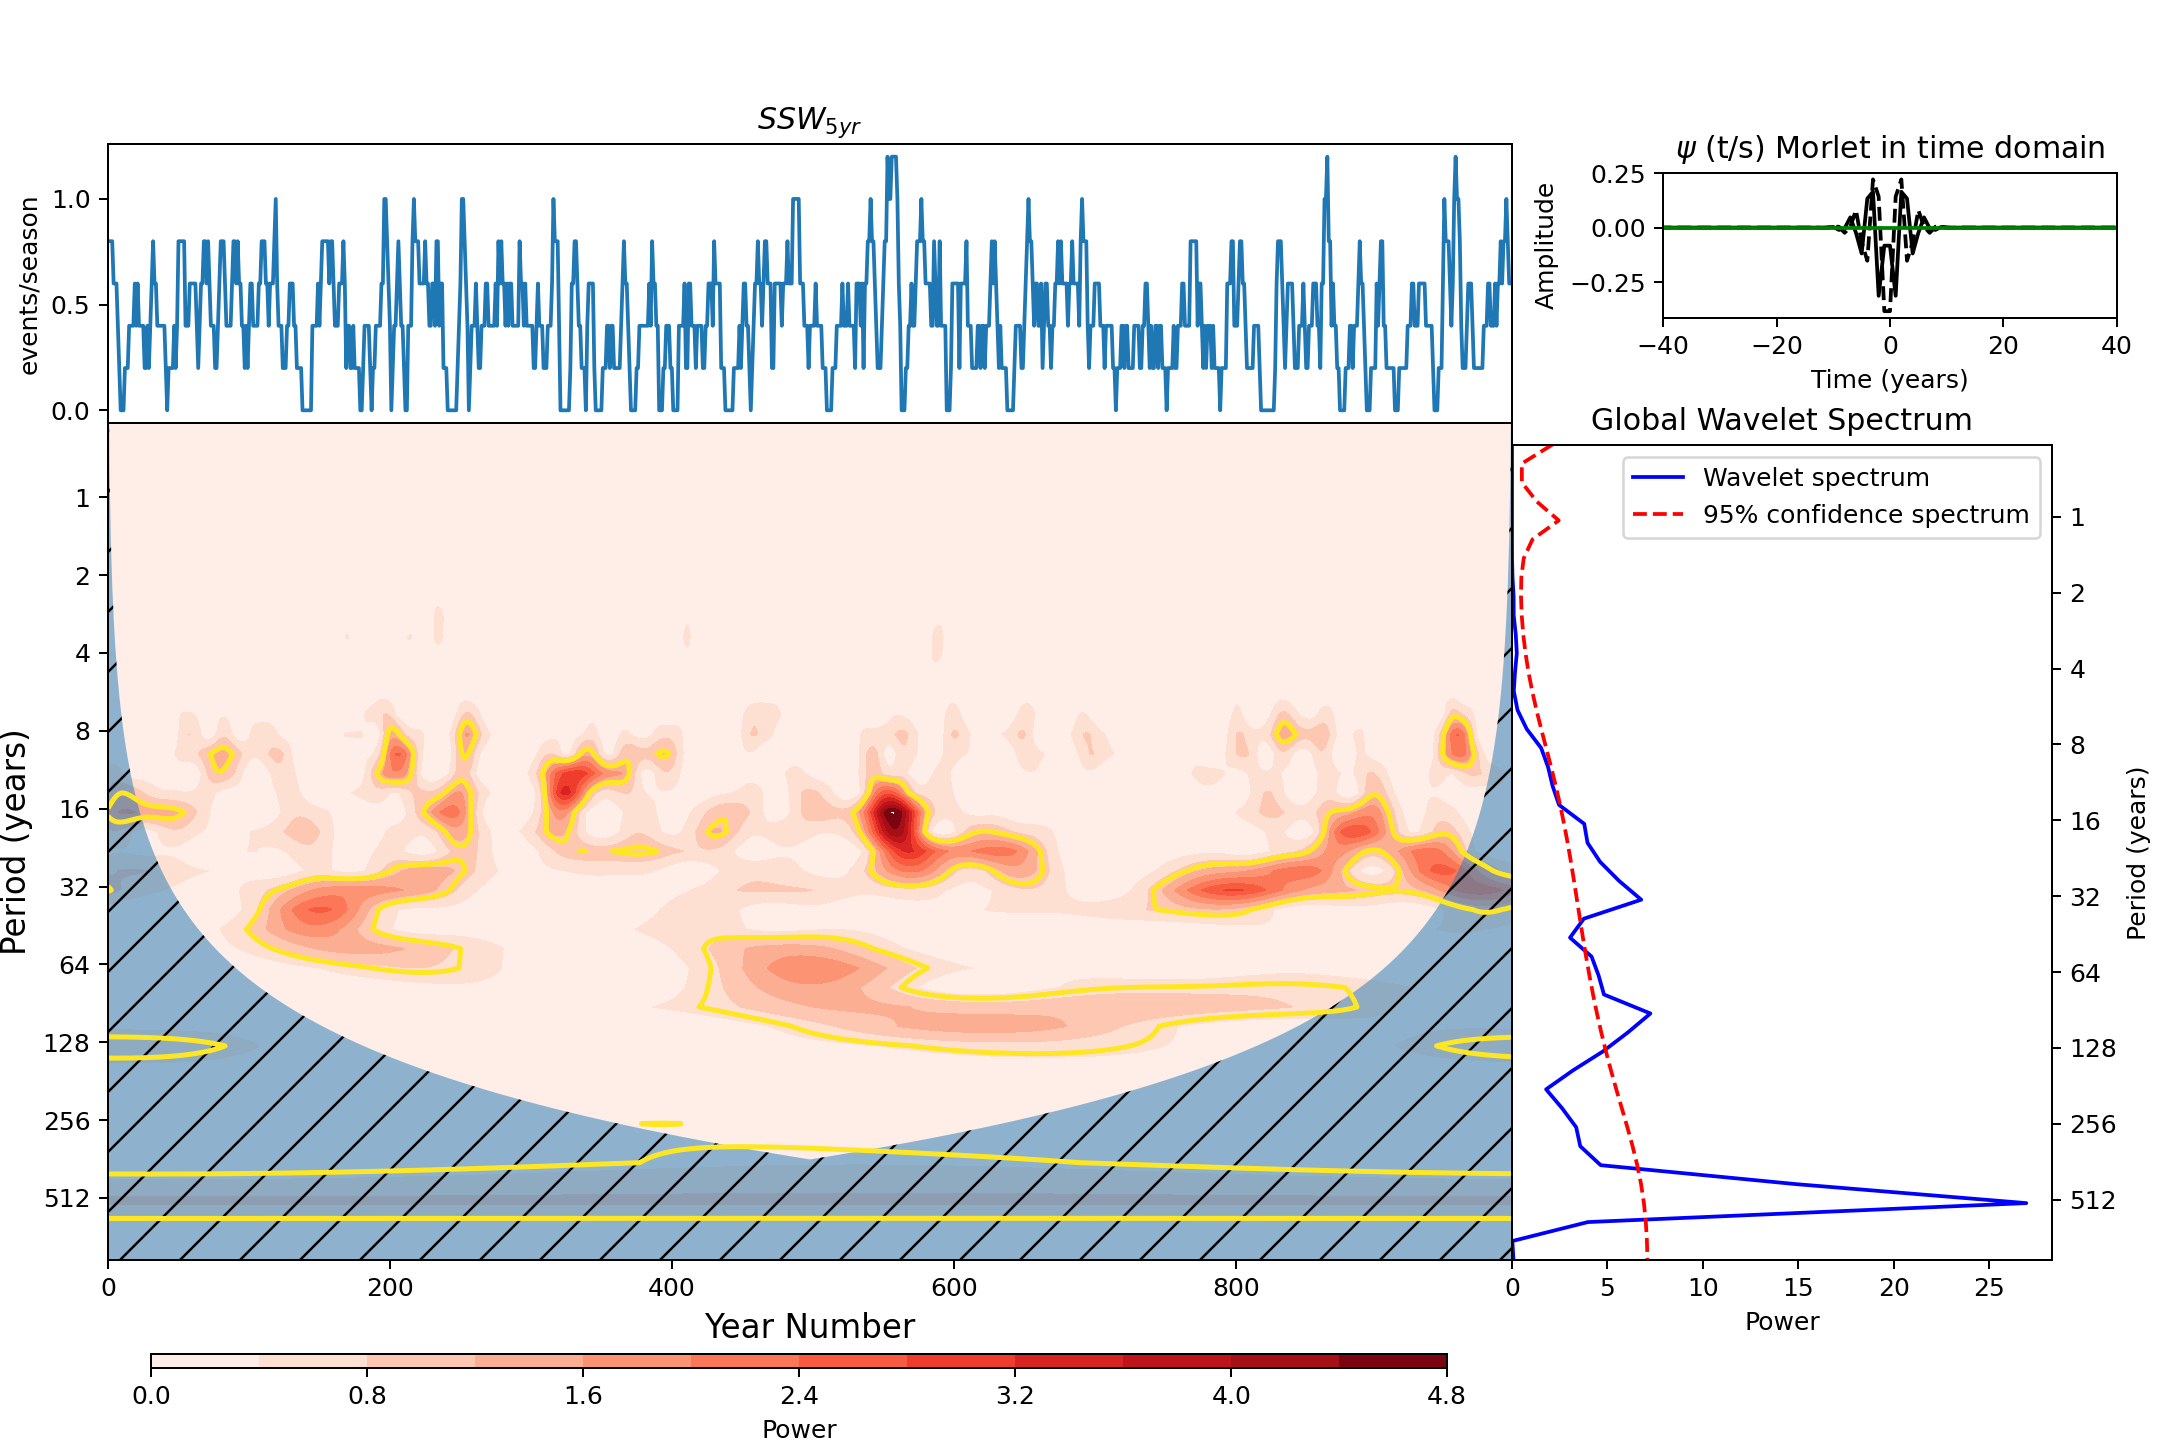
\includegraphics[width = 0.8\linewidth]{Figures/Figures-origins/SSW_wavelet_5_yr_wavelet.png}
\caption[Wavelet power spectrum for Dec-Mar 5 year mean SSW time series]{\textbf{Top left}: SSW events per Dec-Mar season in UKESM smoothed using a 5 year running mean. \textbf{Bottom left}: Wavelet power spectrum of time series in top left. Hatching represents area outside the cone of influence in which edge effects are significant and power should not be considered. Navy contours represent 95\% confidence level assuming mean background AR1 red noise. \textbf{Top Right}: Morlet wavelet used for the wavelet transform in the time domain. \textbf{Bottom right:} Global power spectrum, the wavelet power averaged over the whole simulation, and global 95\% confidence spectrum.}
\label{fig:SSW_series_5yr_wavelet}
\end{center}
\end{figure}

%---------------------------------------------------------------
The wavelet power spectrum of $SSW_{5yr}$ (figure \ref{fig:SSW_series_5yr_wavelet}) shares many of the characteristics of the spectra of the un-smoothed series (figure \ref{fig:SSW_series_wavelet}), but the longer period signals are now more clearly evident, as expected. The $SSW_{5yr}$ wavelet spectrum shows the two broad regions of statistically significant maxima corresponding to signal periods of $\sim$20-30 years and $\sim$60-90 years, but with increased significance both locally and in the time-average. For example, the feature around 90 year period appears significant for 450 years in $SSW_{5yr}$ compared to 350 years before smoothing. One possible explanation for this increase lies in our definition of the significance level on power which is dependent on the lag-1 autocorrelation of the time-series. Introducing a 5 year averaging window will increase the autocorrelation, possibly leading to a less strict significance level. However, this is unlikely because the significance level is constructed using a red noise process with the same autocorrelation as the series. This means that for $SSW_{5yr}$, the threshold for 95\% confidence level increases with increasing period more steeply than in the un-smoothed case and yet the power exhibited at those long periods in $SSW_{5yr}$ nevertheless achieves higher statistical significance. This indicates that the smoothing has enhanced the visibility of a real signal in the $SSW_{5yr}$ time series that was less visible in the un-smoothed time-series. As a check for robustness, we also include the $SSW_{5yr}$ wavelet spectrum including the over-represented November SSW events (figure \ref{fig:SSW_series_5yr_NDJFM_wavelet}). it looks similar to  the spectrum shown in figure \ref{fig:SSW_series_5yr_wavelet} but contains more persistent power on the 8-32 year timescales. The feature noted about on the Dec-Mar $SSW_{5yr}$ wavelet spectrum on $\sim$60-90 years timescales is also present with persistent power for around 450 years of the simulation at these periods. We proceed with the Dec-Mar SSWs for the analysis of possible drivers of this variability as the cause of the November SSW bias in the model is not fully understood and may make attribution of signals more difficult. 


\begin{figure}[h!]
\begin{center}
\noindent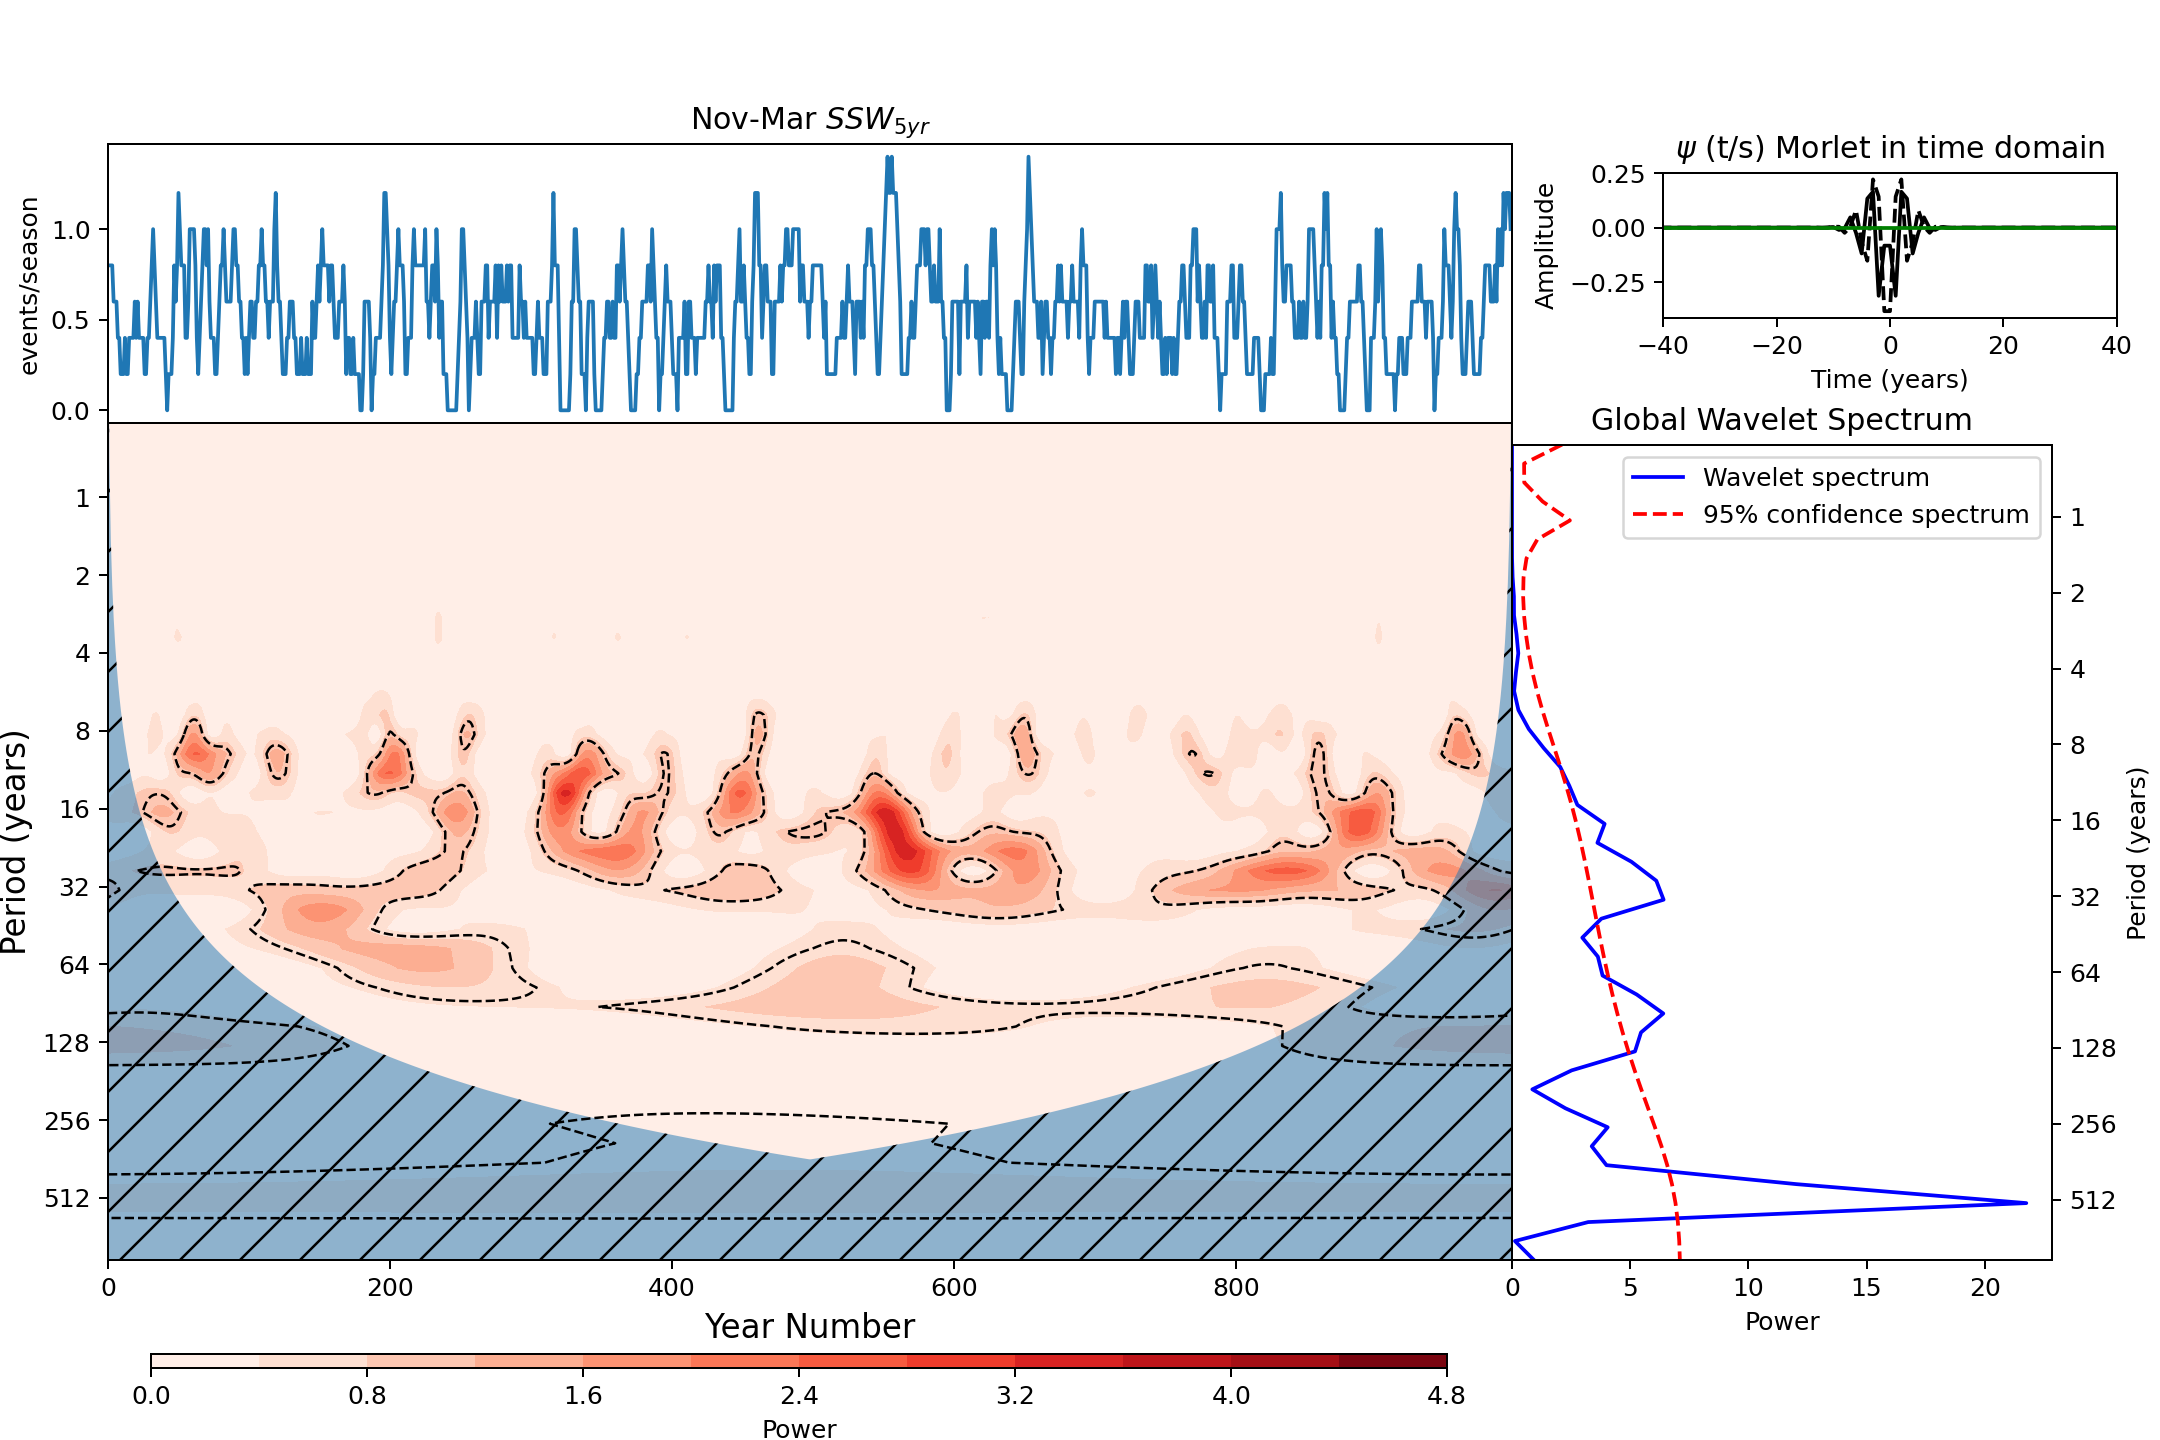
\includegraphics[width = 0.8\linewidth]{Figures/Figures-origins/SSW_wavelet_5_yr_NDJFM.png}
\caption[Wavelet power spectrum of Nov-Mar 5 year mean SSW time series)]{Like figure \ref{fig:SSW_series_5yr_wavelet} for the Nov-Mar SSWs per NH winter season timeseries smoothed with a 5 year rolling window.}
\label{fig:SSW_series_5yr_NDJFM_wavelet}
\end{center}
\end{figure}

%---------------------------------------------------------------


\section{Surface Forcing of Polar Vortex Variability}
In the absence of external forcing mechanisms such as greenhouse gas or anthropogenic aerosol forcing, the presence of long-term variability such as the 60-90 year periodicity seen in $SSW_{5yr}$ (figure \ref{fig:SSW_series_5yr_wavelet}) suggests a source of long-term internal variability from within the climate system. 

The most obvious potential driver of such long timescale variability is the ocean due to its high degree of thermal inertia. Previous work has identified coupling between tropical SSTs and the polar vortex, such as the relationship to ENSO conditions (see section \ref{sec:external_influence_SSTs}). The model exhibits an expected connection between ENSO and the vortex on interannual timescales indicated by the regression analysis results (table 1) and ZMZW composites for El Ni\~{n}o and La Ni\~{n}a winters (figure \ref{fig:ZMZW_comp_ENSO_AL}a, b). Figure \ref{fig:ENSO_wavelet} shows the wavelet power spectrum for the 5 year smoothed Sep-Nov ENSO 3.4 index as well as the cross power spectrum with $SSW_{5yr}$. We use the early NH winter ENSO index to capture the lagged response of the vortex to this mode of variability. The ENSO index is slowly varying so will likely remain in the same state between early and mid-winter. We also smooth the ENSO index for the purposes of calculating the cross spectrum with $SSW_{5yr}$. (The spectrum of the un-smoothed Ni\~{n}o3.4 index is provided in figure \ref{fig:ENSO_unsmoothed_wavelet} and shows significant power in the expected period range of 4-7 years \citep{santosoDefining2017b}). The smoothed ENSO 3.4 index shows intermittent power at periods around 16 years which appears significant in the global spectrum. It also exhibits a small signal coincident with the 90 year variability in $SSW_{5yr}$, however this feature only persists for around 100 years of the simulation. Cross spectra between the two series (figure \ref{fig:ENSO_wavelet}b) reveals that the coincidence in signals at the 90 year period, while significant under our test, is marginally prominent but only covers a small proportion of significant signals in $SSW_{5yr}$. This suggests there may be some contribution from ENSO to the observed SSW variability but it is only marginally significant and on its own it cannot explain the signal in $SSW_{5yr}$ that persists for 450 years. The source of this ENSO signal at 90 year periods is unclear, although the PDO spectrum shares some of the same characteristics on the 90 year timescale (supp figure A4) which is consistent with results of \cite{newmanPacific2016} which proposes the PDO as a low pass filtered version of ENSO. 

\begin{figure}[h!]
\begin{center}
\noindent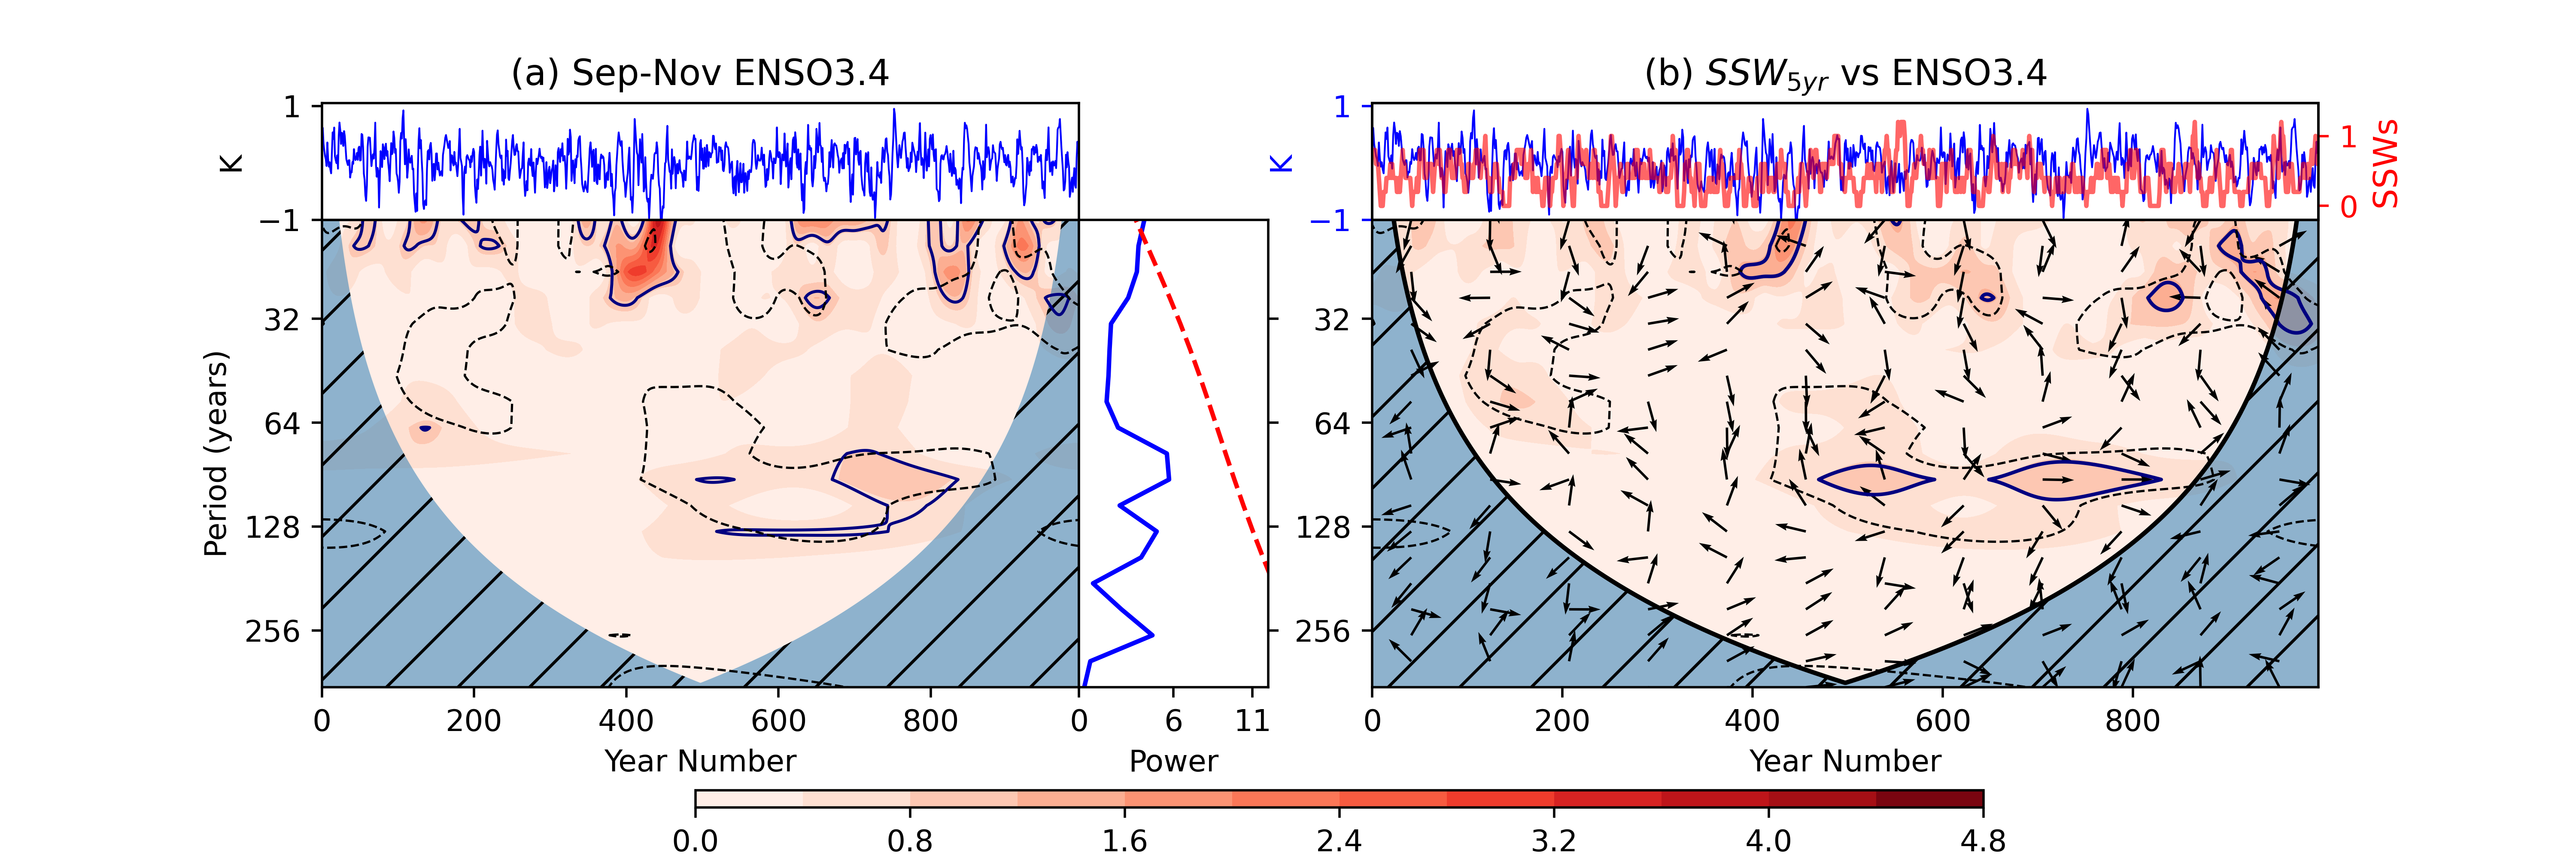
\includegraphics[width = \linewidth]{Figures/Figures-origins/ENSO_wavelet_combined.png}
\caption[Wavelet power spectrum for5 year smoothed Ni\~{n}o3.4 index and cross power spectrum with SSW$_{5yr}$]{\textbf{(a, top)}: Ni\~{n}o3.4 time series, \textbf{a, bottom left}: Wavelet power spectrum (shaded contours represent wavelet power and navy contours the 95\% significance level compared to an AR1 process), \textbf{a, bottom right}: global wavelet power spectrum (blue) and 95\% confidence level (dashed red). \textbf{b}: Cross spectra between $SSW_5yr$ and the Ni\~{n}o3.4 index. \textbf{b, top}: Ni\~{n}o3.4 and $SSW_5yr$ time series. \textbf{b, bottom}: Cross power spectrum. Shading indicates cross power, navy contours the 95\% confidence interval and arrows the relative phase angle between signals in the time series (to the right: in phase, vertically upwards: $\frac{\pi}{2}$ out of phase with SSWs leading, to the left: $\pi$ out of phase, vertically downwards: $\frac{\pi}{2}$ out of phase Ni\~{n}o3.4 leading). Black, dashed contours on both spectra represent the 95\% confidence intervals for the wavelet power spectrum of $SSW_{5yr}$.}
\label{fig:ENSO_wavelet}
\end{center}
\end{figure}

\begin{figure}[h!]
\begin{center}
\noindent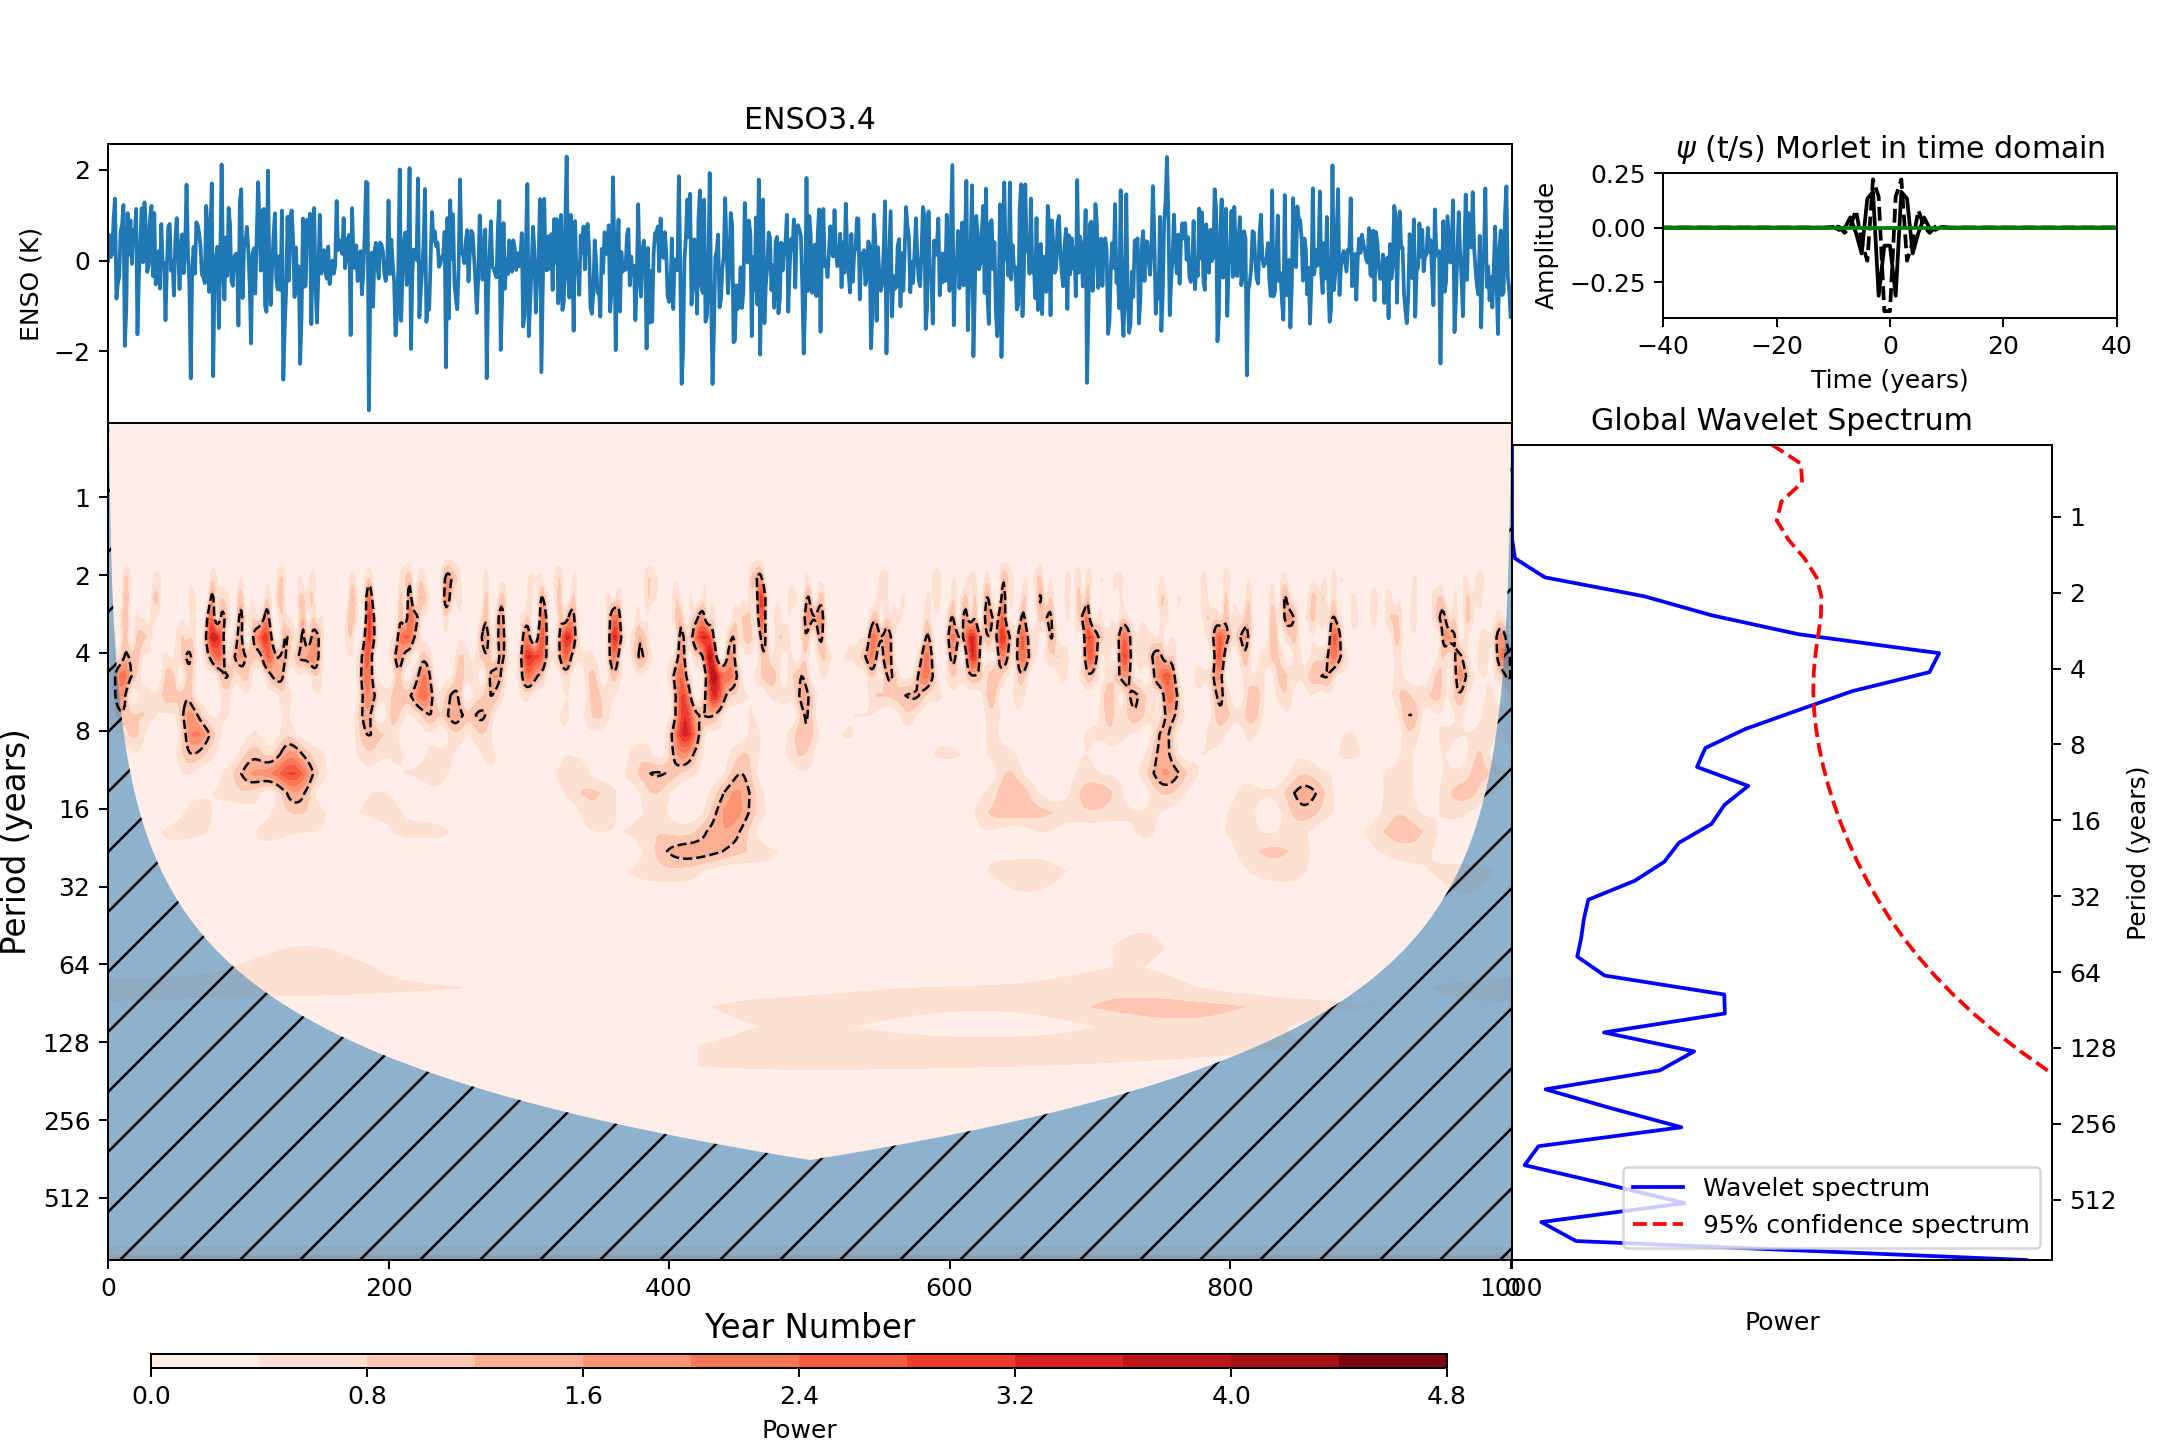
\includegraphics[width = \linewidth]{Figures/Figures-origins/ENSO_wavelet_unsmoothed.png}
\caption[Wavelet power spectrum of the Ni\~{n}o3.4 index]{Like figure \ref{fig:SSW_series_wavelet} for the Sep-Nov  Ni\~{n}o3.4 index} 
\label{fig:ENSO_unsmoothed_wavelet}
\end{center}
\end{figure}

In the interest of completeness, we also explore the long-term variability of other tropical ocean regions and their potential teleconnections with the polar vortex. Four additional tropical regions were selected based on those identified by \cite{scaifeTropical2017b} and outlined in section \ref{sec:model_diagnostics}. While all four regions show some elements of multi-decadal variability (figure \ref{fig:tropical_SST_wavelet}), particularly the Tropical Atlantic with a peak period of approximately 140 years for 700 years of the simulation, none of the spectra show variability that coincides well with that of $SSW_{5yr}$. There is some overlap of the Atlantic and Tropical East Pacific spectra with the regions of significant periodicity at around 60-90 years in the $SSW_{5yr}$ spectrum but, like the Ni\~{n}o3.4 index, the overlaps between the series are minimal and cannot reasonably explain the vortex signal, especially the signal of period approximately 90 years that persists in $SSW_{5yr}$ for around 450 years (figure \ref{fig:tropical_SST_wavelet} dashed contours).

\begin{figure}[h!]
\begin{center}
\noindent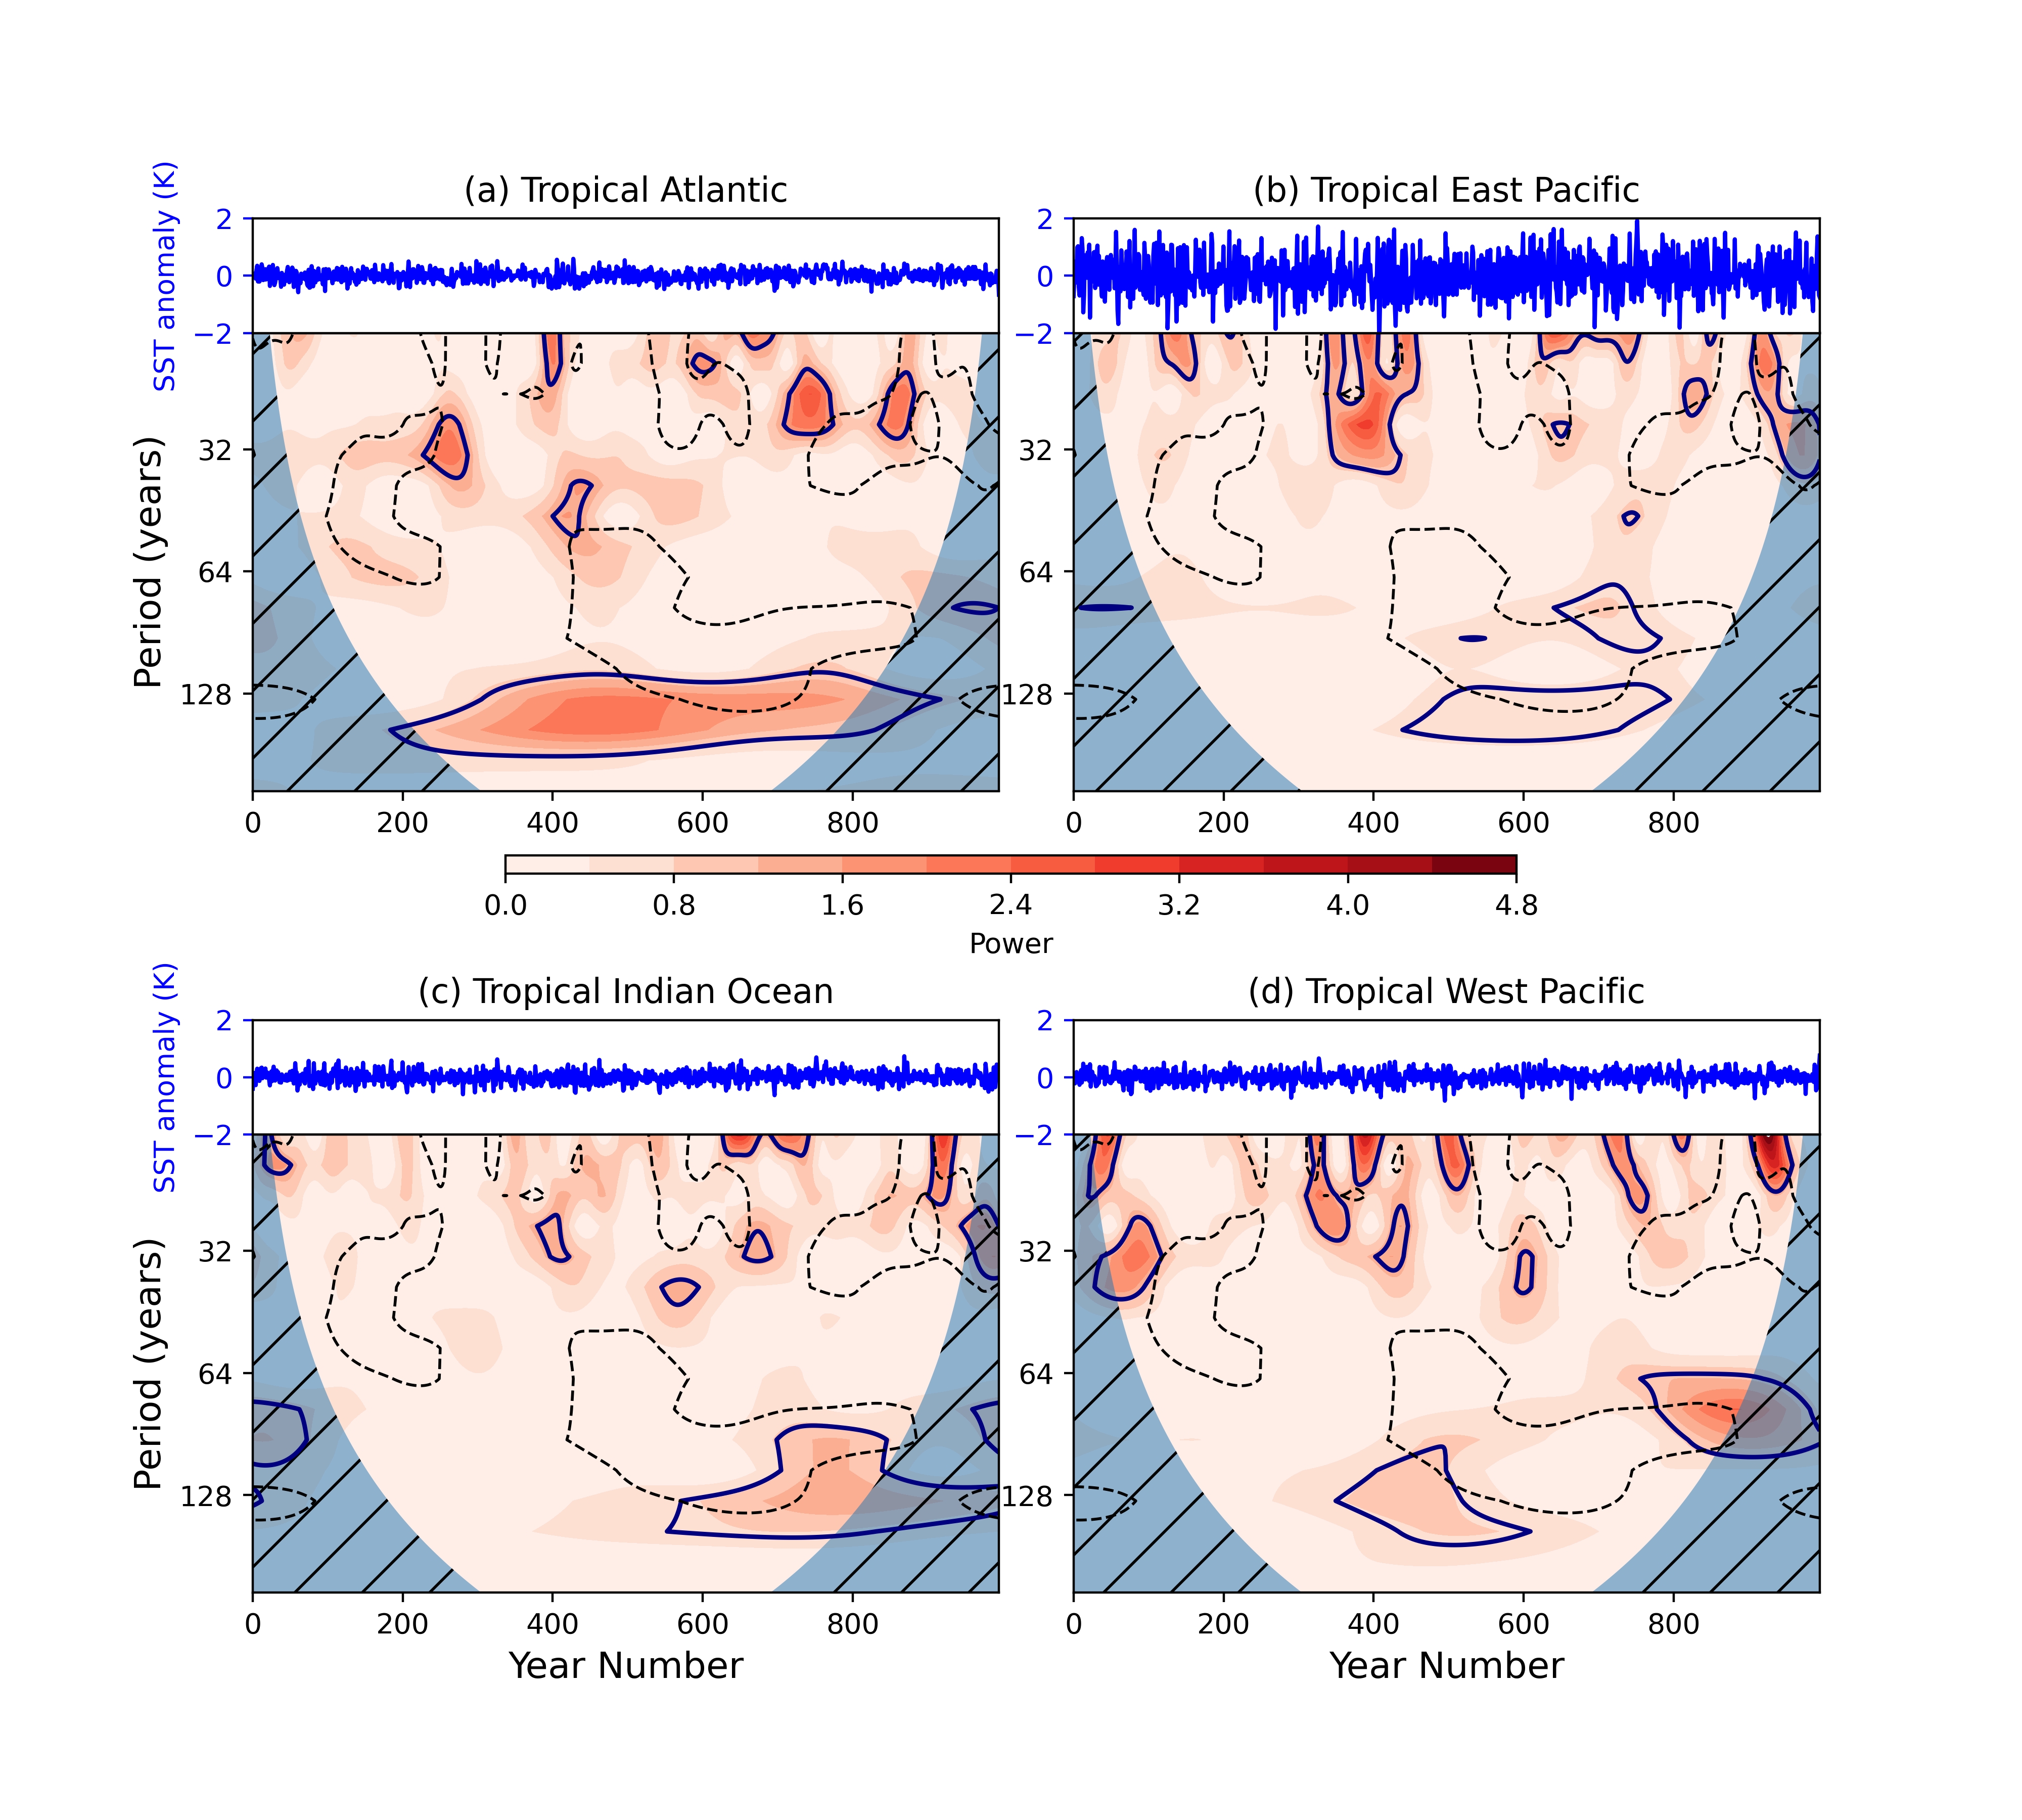
\includegraphics[width = 0.8\linewidth]{Figures/Figures-origins/SSTs_tropical_wavelet.png}
\caption[Wavelet power spectra of tropical basin SST indices.]{Sep-Nov SST anomaly time series and associated wavelet power spectrum for Tropical Atlantic (5$^{\circ}$\,S–5$^{\circ}$\,N, 60$^{\circ}$\,W–0$^{\circ}$\,W), Tropical East Pacific (5$^{\circ}$\,S–1$^{\circ}$\,N, 160$^{\circ}$\,E–270$^{\circ}$\,E), Tropical West Pacific (5$^{\circ}$\,S–25$^{\circ}$\,N, 110$^{\circ}$\,E–140$^{\circ}$\,E) and Tropical Indian Ocean (5$^{\circ}$\,S–10$^{\circ}$\,N, 45$^{\circ}$\,E–100$^{\circ}$\,E). Shading indicates wavelet power, yellow contours show the 95\% confidence level when the power is compared to and AR1 red-noise process and dashed contours indicate the 95\% confidence level for the power spectrum of $SSW_5yr$.}
\label{fig:tropical_SST_wavelet}
\end{center}
\end{figure}

The strength of the Aleutian Low (AL) has also been used as an indicator of tropospheric wave forcing and its influence on the polar vortex \citep{wooConnection2015b}. We perform a similar wavelet and cross-spectrum analysis using an index based on the strength of the modelled NH winter (Dec-Mar) AL (see section \ref{sec:model_diagnostics} for details). The wavelet power spectrum for the 5-year smoothed AL index (figure \ref{fig:AL_wavelet}a) exhibits elements of periodic signals with maximum power corresponding to a period of around 55 years (between 40-60 years) but with fairly minimal overlap with the regions enclosed by the 95\% confidence level in the corresponding SSW wavelet analysis (green contours). AL indices derived from different winter months give similar spectral patterns (not shown).  The cross spectrum analysis between the AL and $SSW_5yr$ (figure \ref{fig:AL_wavelet}b) highlights this relatively small region of overlap in the interval between years 400-500. However, the phase relationship, indicated by the arrows in that region of overlap is difficult to interpret. The proposed physical mechanism of coupling between the AL and the vortex \citep{wooConnection2015b} involves an association between a deeper AL (i.e. lower pressure and hence a negative anomaly) with increased frequency of SSWs. This negative correlation would give rise to arrows pointing to the left if the relationship was present. In contrast, the upward arrows in figure \ref{fig:AL_wavelet}b indicate a $\frac{\pi}{2}$ phase difference between the indices on these 60 year timescales, suggesting that peaks in $SSW_{5yr}$ variations are associated with maximum rates of change of the AL index at the same periods. As with Ni\~{n}o3.4, the spectra of the AL shares some features with that of the PDO (figure \ref{fig:PDO_wavelet}). This is consistent with studies into these modes of variability which find significant correlation of the PDO and AL \citep{mantuaPacific1997a, rodionovSpatial2005b} as well as studies that examine influence of PDO on vortex strength through a pathway involving the AL and ENSO \citep{raoModulation2019d}. Despite this possible pathway, the relatively short time interval of overlap between the AL and $SSW_{5yr}$ signals at the 60-yr period, the absence of any significant signal around the 90-yr period, together with the inconsistent phase relationships, points to a conclusion that AL forcing is unlikely to be the primary driver of long-term variability in $SSW_{5yr}$. Indeed, examination of the cross-spectrum between the un-smoothed AL and SSW indices (figure \ref{fig:AL_unsmoothed_wavelet}) shows little indication of a coherent relationship between periodic signals in the two indices at any timescale. Finally, while the regression results of the un-smoothed indices give a significant coefficient for the AL (table 1), its magnitude is small compared to that of Ni\~{n}o3.4 and the deep QBO, the uncertainty on the coefficient is large and the associated p value is close to the 95\% significance boundary. The weak relationship between the AL and SSWs is unexpected due to the well acknowledged influence of the AL over planetary wave flux in the upper troposphere \citep{wooConnection2015b}. To attempt to address this, we also analyse an AL metric evaluated as the area weighted average over a box recommended by \cite{garfinkelWhy2012b} who use an SSW precursor region in 500hPa height defined by $52.5^{\circ}$–$72.5^{\circ}N$, $165^{\circ}$–$195^{\circ}E$. However, we find a lower correlation between this measure and our SSW timeseries than between the original EOF based metric and SSWs ($r = -0.21$ for the EOF based AL and $r = -0.13$ for the box based AL).

%---------------------------------------------------------------

\begin{figure}[h!]
\begin{center}
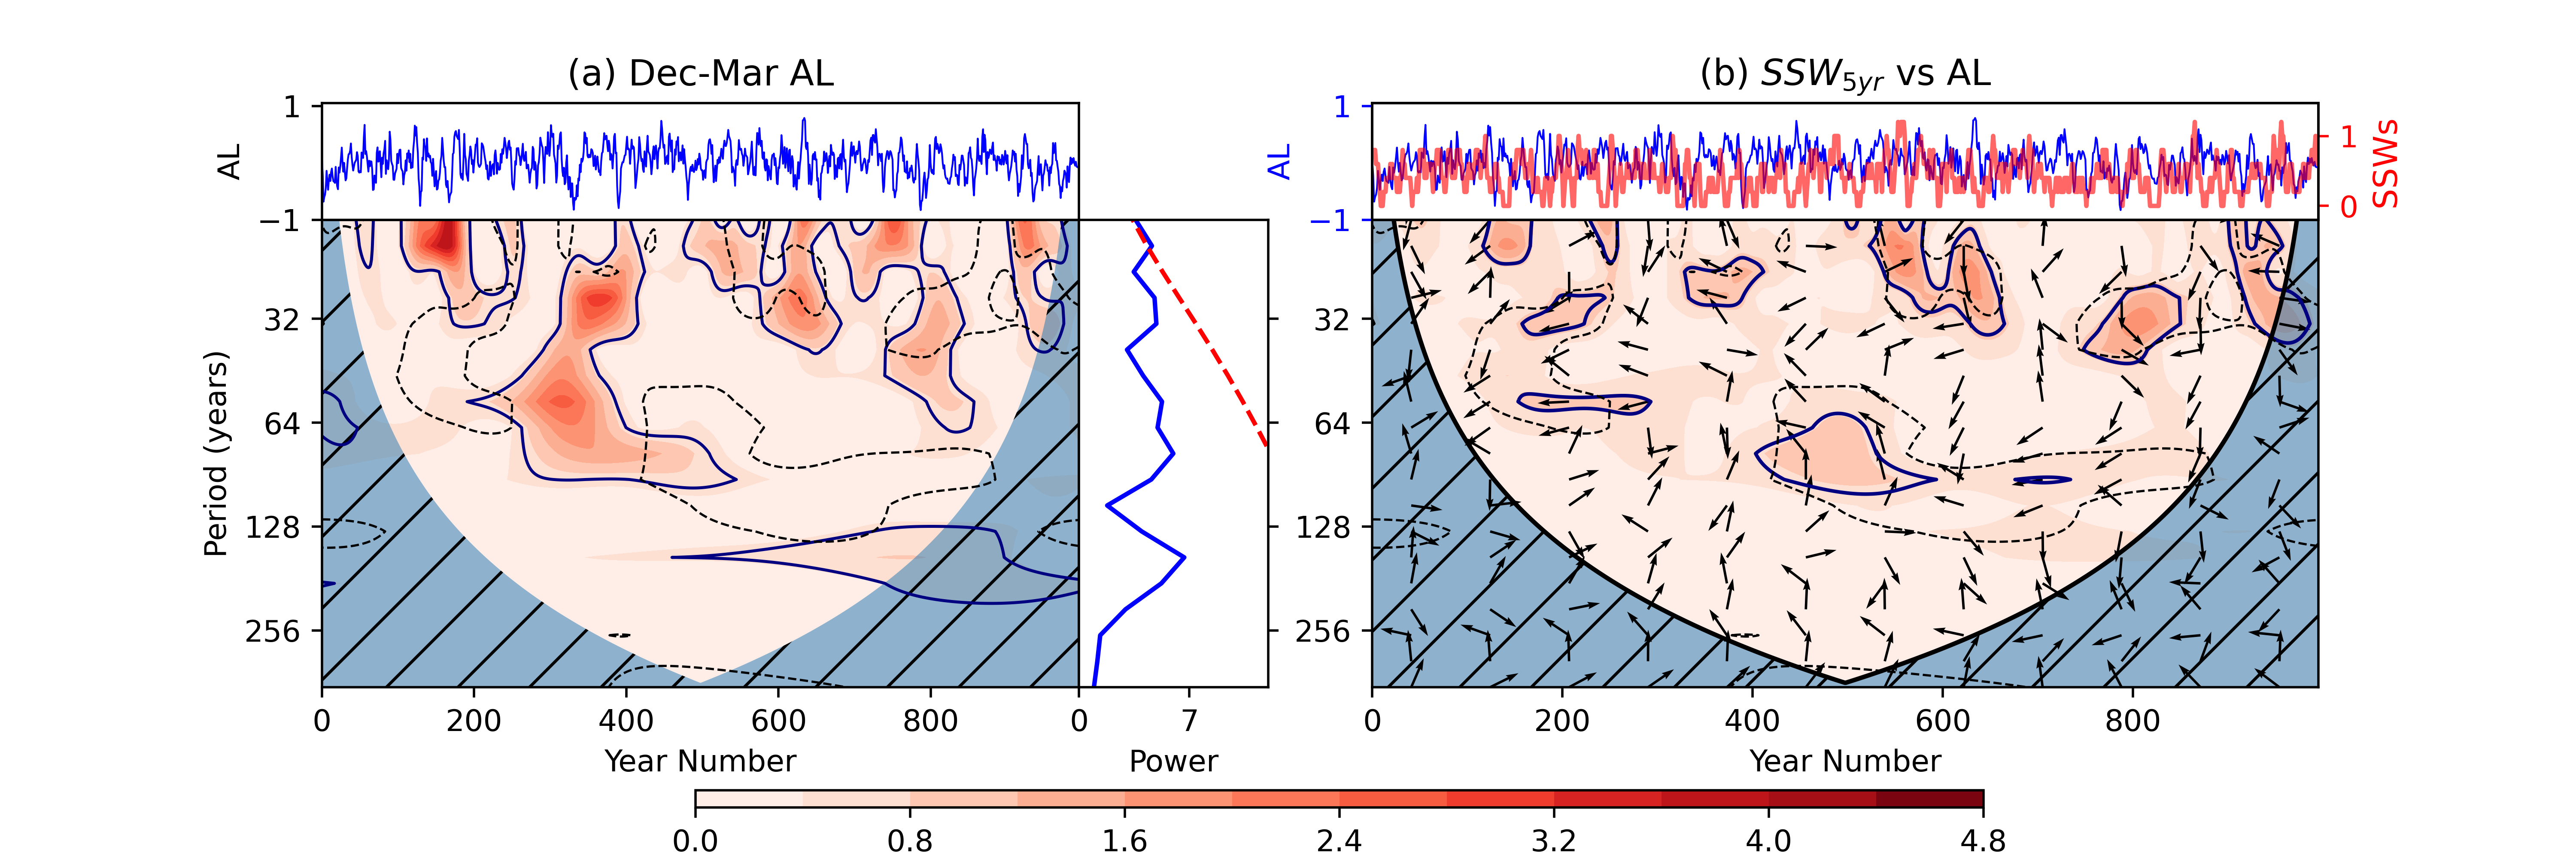
\includegraphics[width = \linewidth]{Figures/Figures-origins/AL_wavelet_combined.png}
\caption[Wavelet power spectrum for 5 year smoothed AL index]{Like figure \ref{fig:ENSO_wavelet} for the Dec-Mar Aleutian Low index smoothed with a 5 year window. \textbf{a}: AL time series and associated wavelet power spectrum. \textbf{b}: Cross power spectrum between AL and $SSW_{5yr}$.}
\label{fig:AL_wavelet}
\end{center}
\end{figure}

\begin{figure}[h!]
\begin{center}
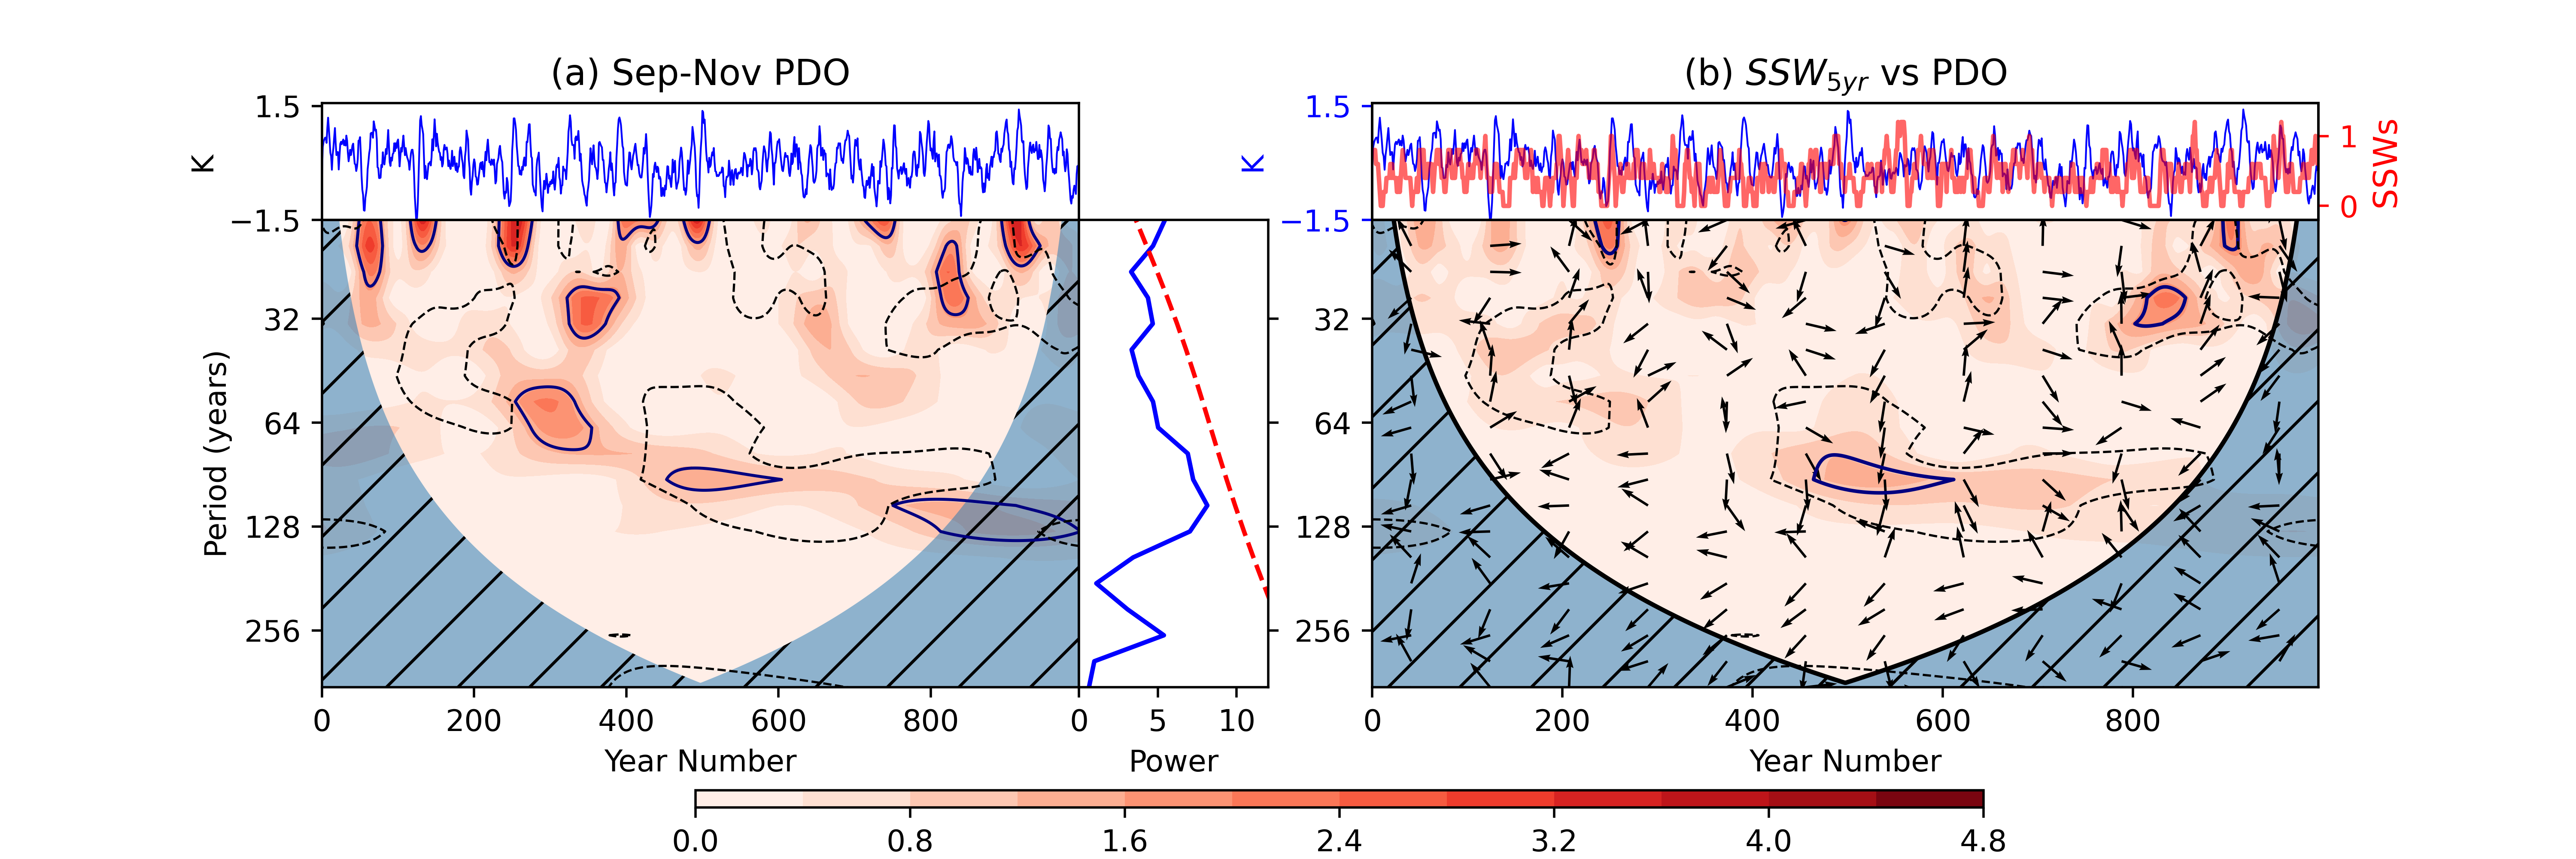
\includegraphics[width = \linewidth]{Figures/Figures-origins/PDO_wavelet_combined.png}
\caption[Wavelet power spectrum for 5 year smoothed PDO index]{Like figure \ref{fig:ENSO_wavelet} for the Sep-Nov PDO index smoothed with a 5 year window. \textbf{a}: PDO time series and associated wavelet power spectrum. \textbf{b}: Cross power spectrum between PDO and $SSW_{5yr}$.}
\label{fig:PDO_wavelet}
\end{center}
\end{figure}

\begin{figure}[h!]
\begin{center}
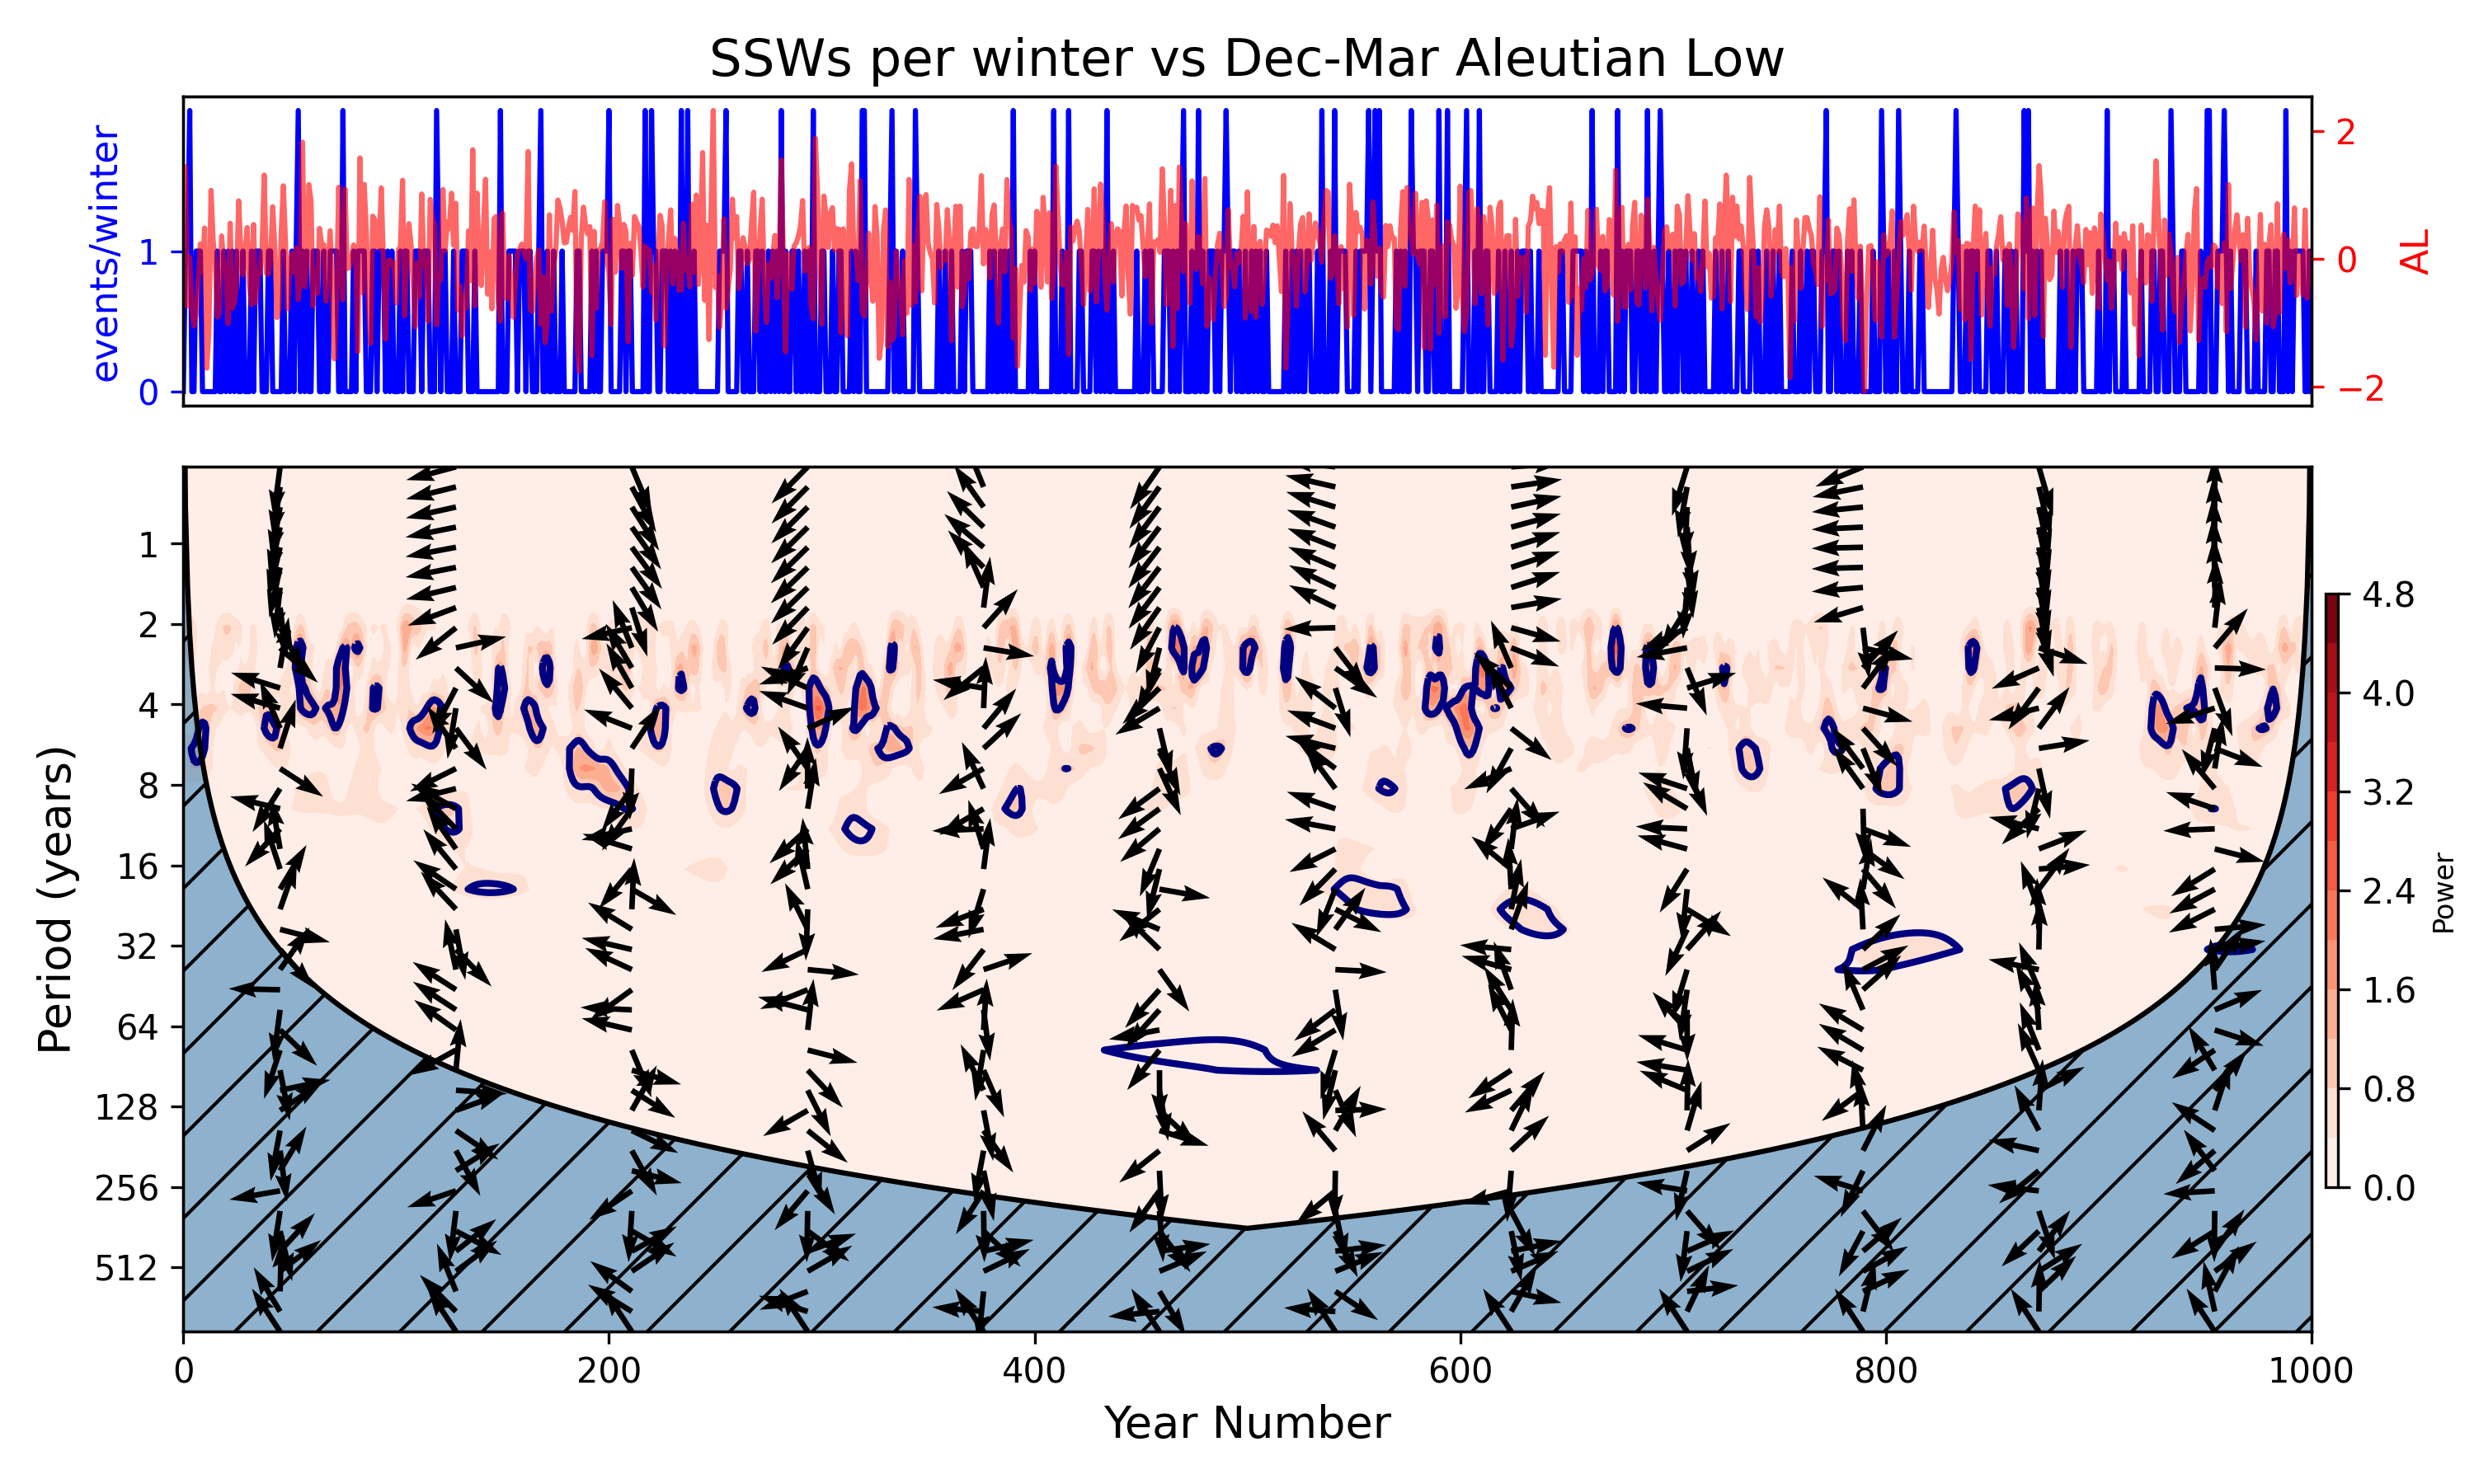
\includegraphics[width = \linewidth]{Figures/Figures-origins/SSWs_vs_AL_wavelet_unsmoothed.png}
\caption[Wavelet cross power spectrum between AL index and SSW timeseries]{\textbf{Top}: December–March Aleutian Low index (red) and SSWs per NH winter (blue) time series. \textbf{Bottom} Cross-wavelet power spectrum between the two time series.}
\label{fig:AL_unsmoothed_wavelet}
\end{center}
\end{figure}

%---------------------------------------------------------------

\section{Vortex-QBO Interactions}
Despite some coincident signals between tropical SSTs, AL and $SSW_{5yr}$, long-term variability in these surface indices are unable to fully account for the  multidecadal signals in SSW frequency. An additional potential source of internally generated long-term variability may reside within the stratosphere. Studies have noted relatively long-term variations in the strength of the Holton-Tan relationship \citep{luDecadalscale2008c,luMechanisms2014c,ospreyClimatology2010b} although the cause of these variations is not well understood. In order to investigate this figure \ref{fig:QBO_levs} shows the wavelet power spectrum of early winter (Sep-Nov) QBO winds evaluated at selected levels. Since the QBO evolves relatively slowly, employing Sep-Nov averaged winds provides a reasonable representation of the QBO and also allows us to evaluate the in-season lagged relationship between the QBO and subsequent occurrence of an SSW. There is a clear signal between 2 and 4 years for the majority of the simulation, as expected, but no prominent power at longer periods,  confirming that there is no significant long-term variability in the periodicity of the QBO winds that could explain the long-term variations in $SSW_{5yr}$ via the Holton-Tan relationship.

\begin{center}
\begin{figure}[h!]
\noindent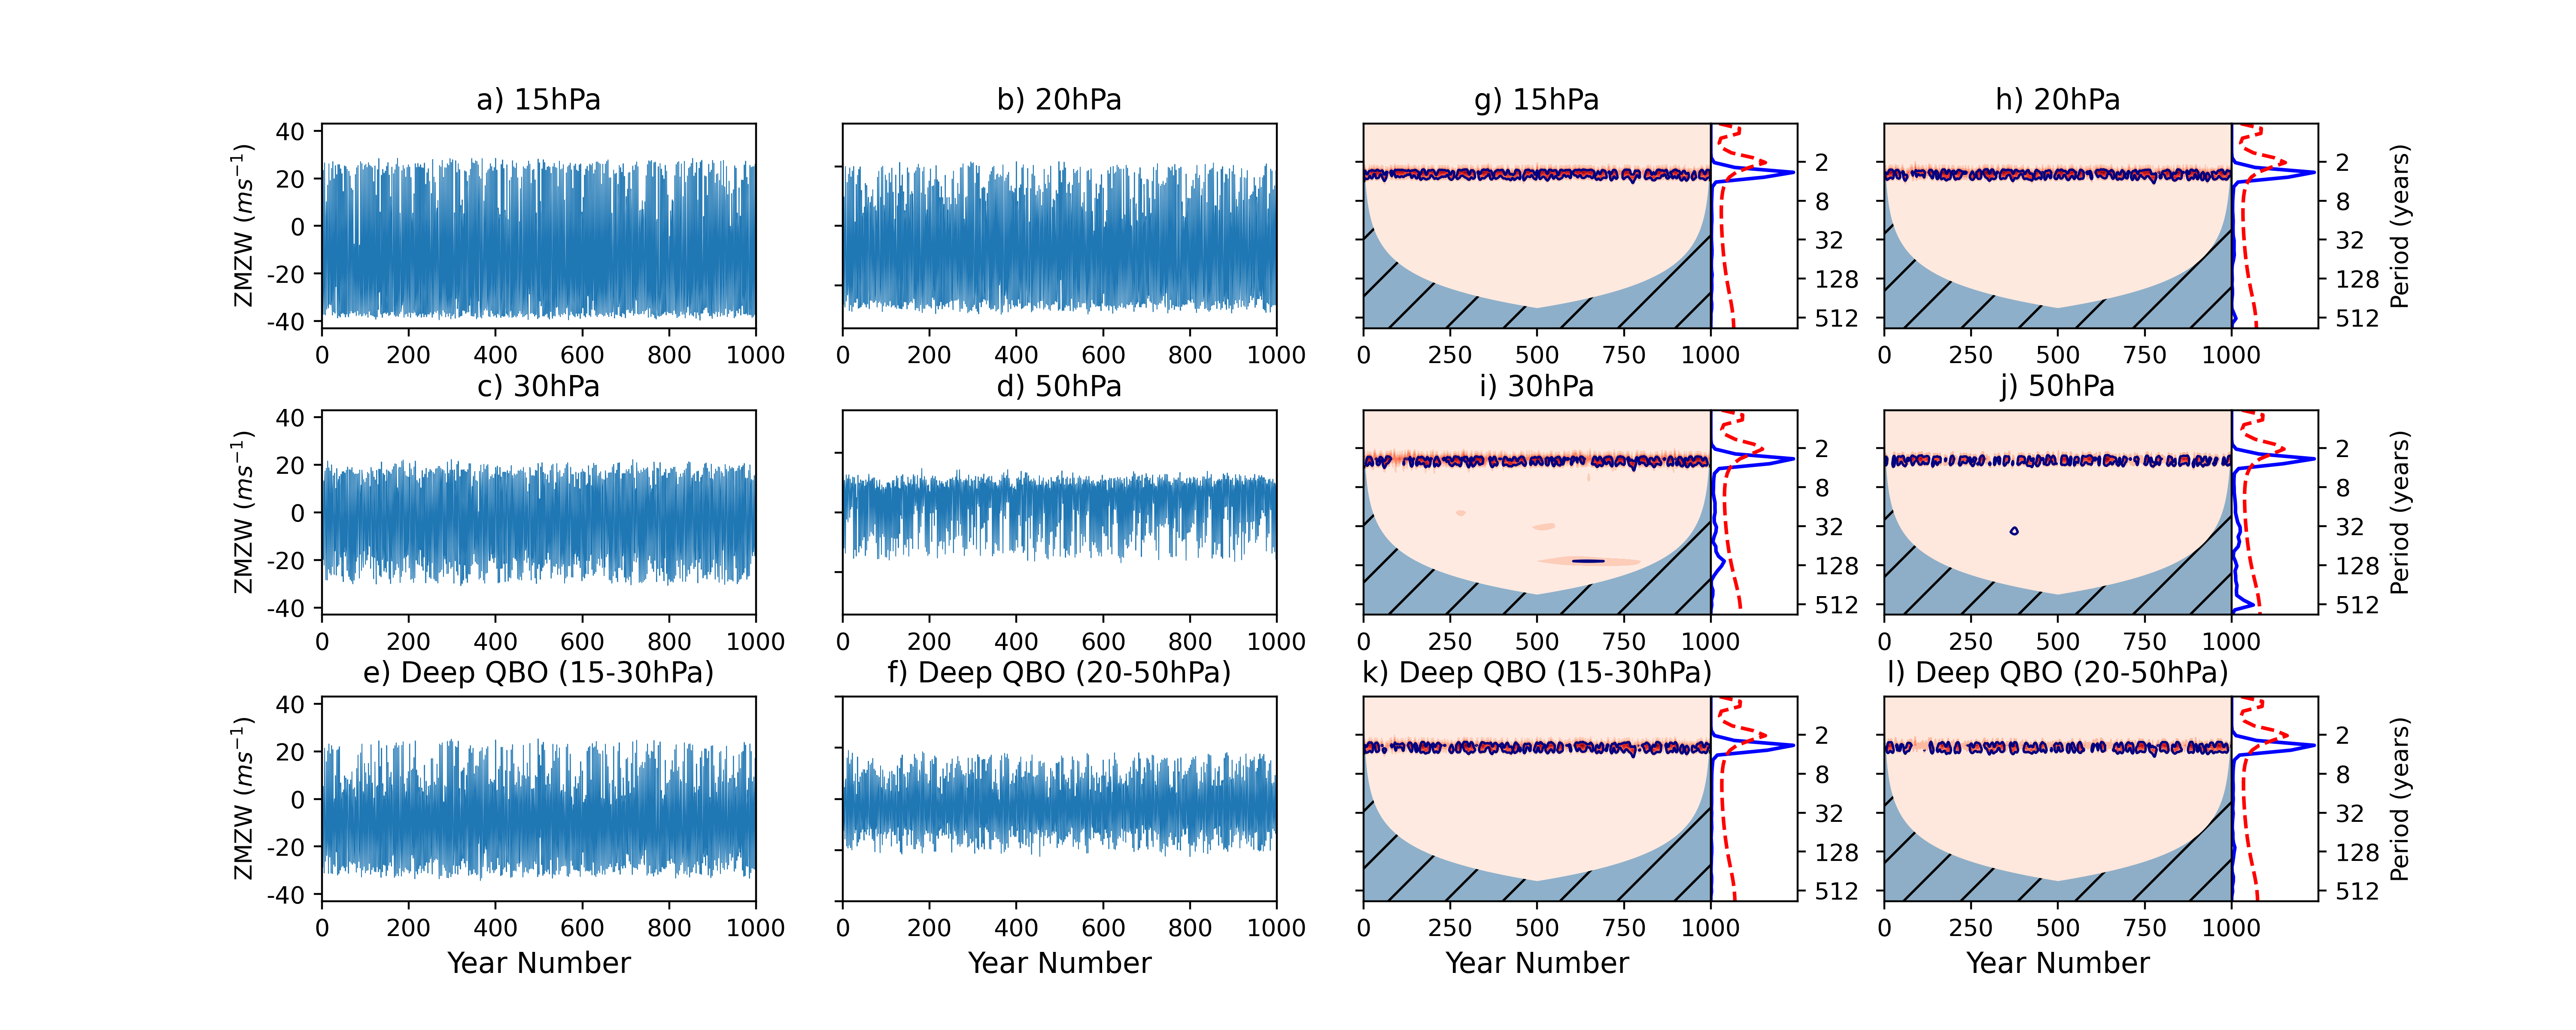
\includegraphics[width = \linewidth]{Figures/Figures-origins/QBO_levels.png}
\caption[QBO timeseries and associated wavelet power spectra at different levels in UKESM]{\textbf{(a-f)}: Sep-Nov mean ZMZW averaged between 5$^\circ$S--5$^\circ$N latitude on different pressure levels (a-e) and the deep metric averaged between 15--30\,hPa (f). \textbf{(g-l)}: Wavelet power spectra for each time series shown in (a-c). Shading represents wavelet power with a colour scale the same as that seen in figure \ref{fig:SSW_series_5yr_wavelet} and navy contours indicate regions of significant power (>95\% confidence interval) compared to a background AR1 process.}
\label{fig:QBO_levs}
\end{figure}
\end{center}

%---------------------------------------------------------------

While the wavelet analysis technique is able to isolate and reveal frequency modulations very well it is less suited to examine amplitude modulations which are clearly evident by eye in some of the QBO index time-series. For example, both the 20 hPa and deep (15-30 hPa) QBO time series show multi-decadal variations in the magnitude of the westerly phase while the easterly phase amplitudes are relatively uniform in time. Similarly, the 50\,hPa and 30\,hPa time series show amplitude modulation predominantly in the easterly phase. This amplitude modulation can be highlighted by taking the Hilbert Transform of each QBO time-series (figure \ref{fig:QBO_levs_amp}a-f). Wavelet analysis of the transformed QBO time series now shows significant power on multidecadal timescales (figure \ref{fig:QBO_levs_amp}g-l). In particular, the 20\,hPa and deep QBO time-series exhibit signals coincident in time and around similar periods (60-90 years) to those observed in $SSW_5yr$. On the other hand, the QBO indices based on equatorial winds at 50\,hPa or 30\,hPa show minimal power at these periods, despite showing a strong intraseasonal HT relationship (figure \ref{fig:holton_tan_comp}). Given that the 15-30 hPa deep QBO  index exhibits  both multidecadal timescale variability and a strong intraseasonal HT coupling, we continue further analysis of the SSW-QBO interactions using the 15-30 hPa index. 

%---------------------------------------------------------------

\begin{figure}[h!]
    \begin{center}
    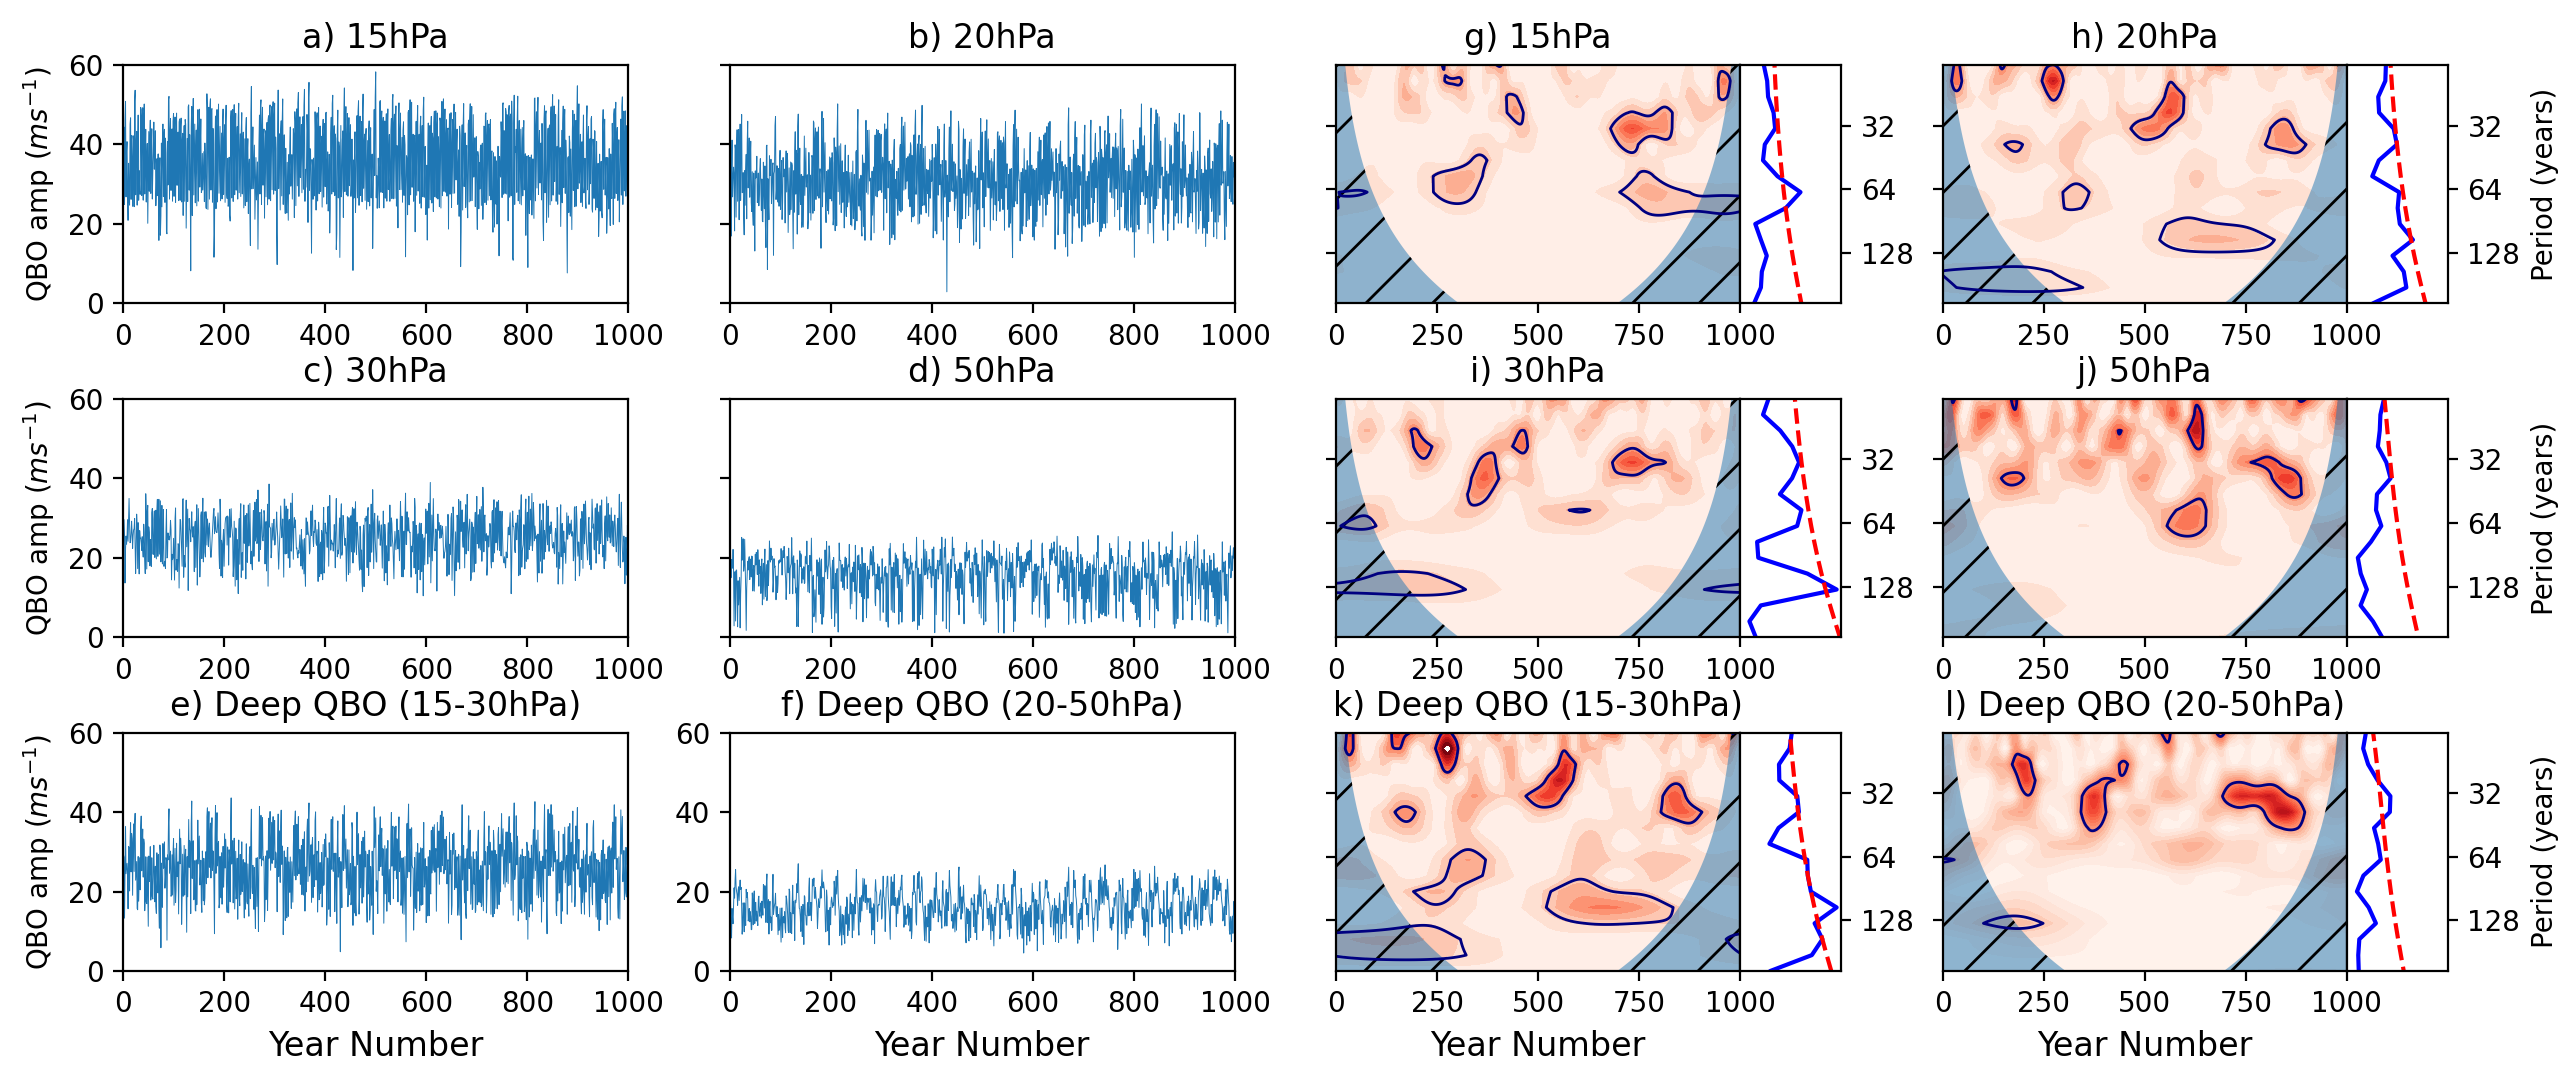
\includegraphics[width = \linewidth]{Figures/Figures-origins/QBO_levels_amp.png}
    \caption[QBO amplitude timeseries and associated wavelet power spectra at different levels in UKESM]{\textbf{(a-e)}: Hilbert amplitude of Sep-Nov mean ZMZW averaged between 5$^\circ$\,S--5$^\circ$\,N latitude on different pressure levels (a-e) and the deep metric averaged between 15--30\,hPa (f). \textbf{(g-l)}: Wavelet power spectra for each time series shown in (a-c). Shading represents wavelet power with a colour scale the same as that seen in figure \ref{fig:SSW_series_5yr_wavelet} and navy contours indicate regions of significant power (>95\% confidence interval) compared to a background AR1 process.}
    \label{fig:QBO_levs_amp}
    \end{center}
\end{figure}

%---------------------------------------------------------------

Wavelet analysis of the 5-year smoothed deep (15-30\,hPa) QBO amplitude modulation index (figure \ref{fig:QBO_SSW_subfig}a) enhances the clarity of the long-term periodicity, showing statistically significant power at around 90 years in the interval between year numbers 500-800. The cross power between $SSW_5yr$ and this QBO amplitude modulation index (figure \ref{fig:QBO_SSW_subfig}) coincides extremely well with the signals observed in $SSW_5yr$ at around 90 years. There are also coincident features at other timescales, although the feature between years 450-550 at periods of 60 years is less well captured. The phase-relationship arrows in the main region of long-term variability (periods around 90 years in the interval 450-800 years) point broadly to the left ($\pi$ phase shift), indicating that the signals are approximately anti-phased (the slight downward pointing of the arrows suggests a small deviation from this lag-zero relationship and is discussed below). The anti-phase relationship is consistent with the HT relationship in which a westerly (positive) QBO anomaly corresponds to a reduction in the frequency of SSWs.

%---------------------------------------------------------------

\begin{center}
\begin{figure}[h!]
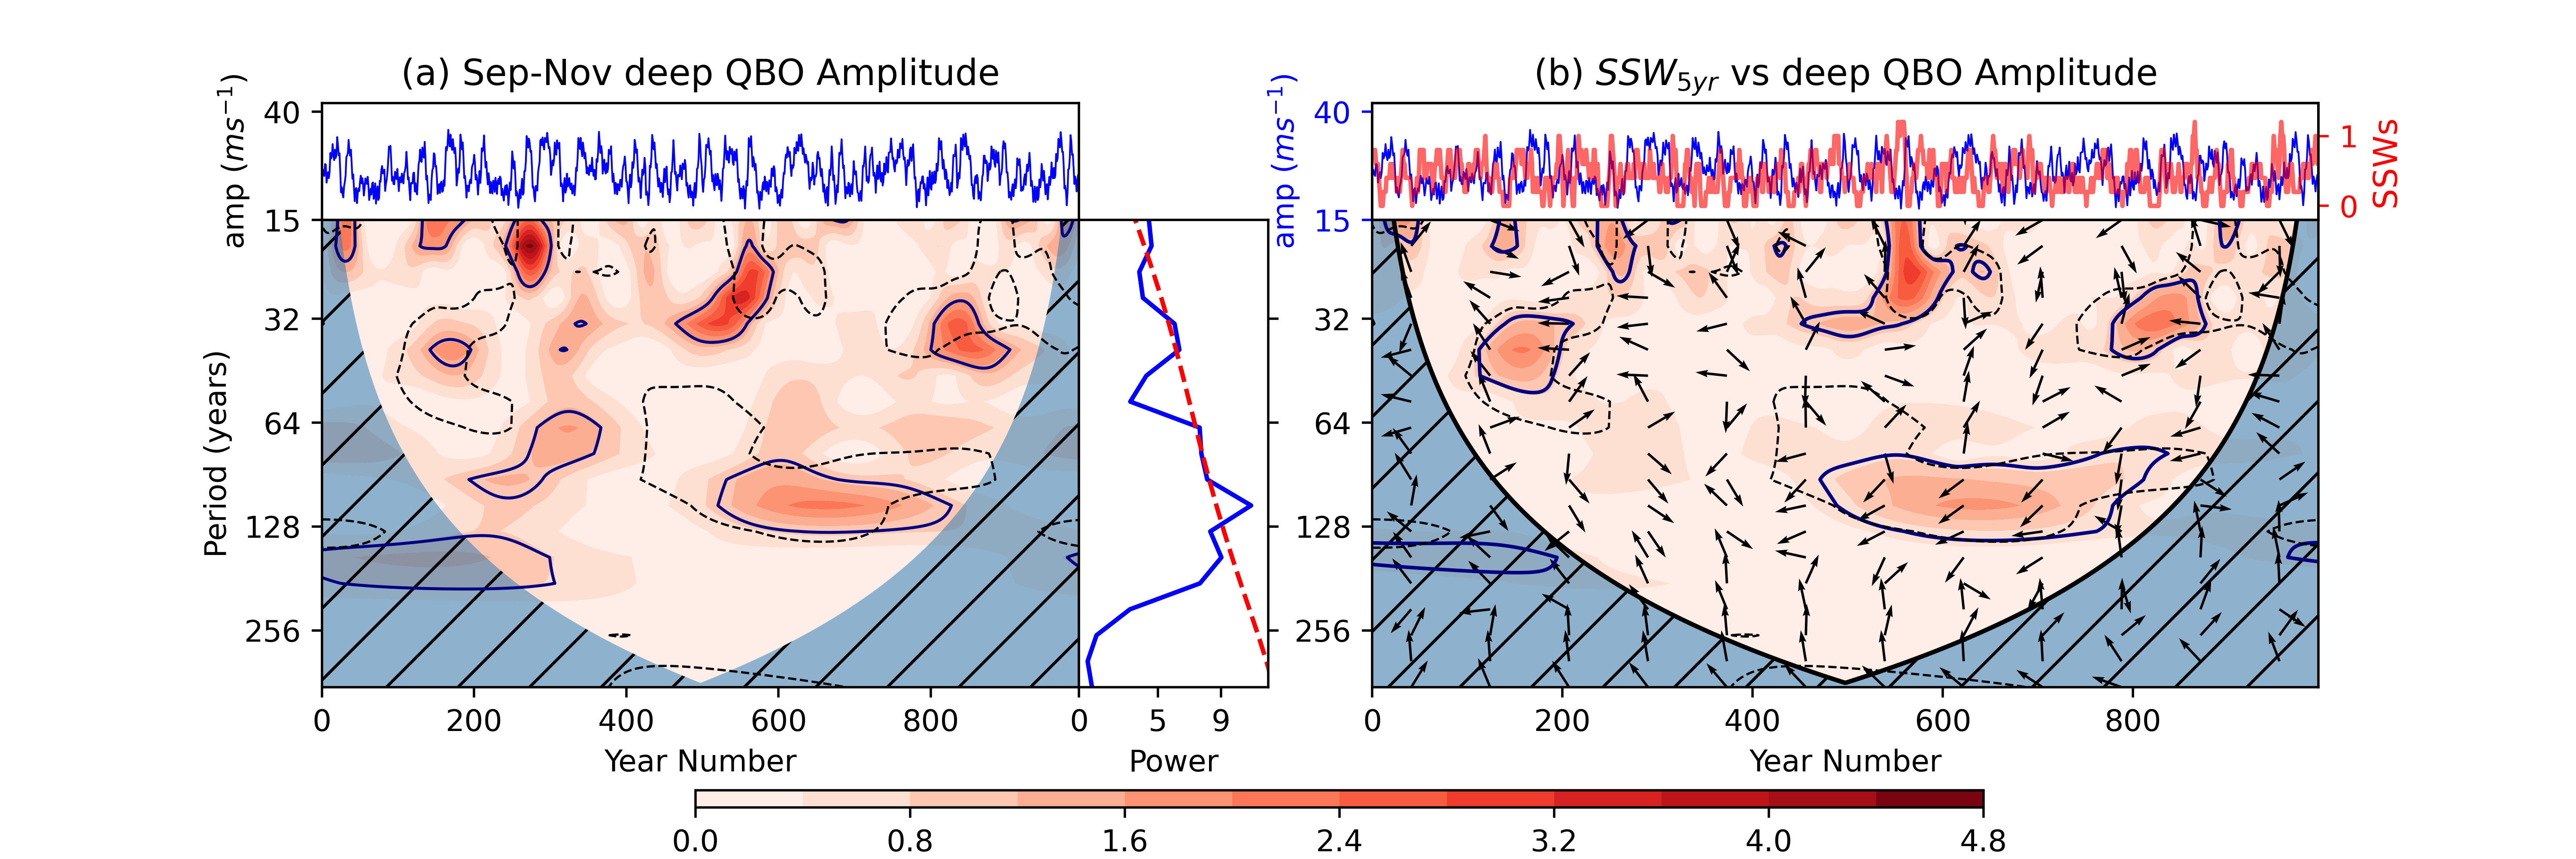
\includegraphics[width = \textwidth]{Figures/Figures-origins/deep_QBO_amp_wavelet_combined.png}
\caption[Wavelet and cross spectra for the deep QBO amplitude in UKESM.]{Like figure \ref{fig:ENSO_wavelet} for the Sep-Nov deep QBO (15--30\,hPa) amplitude index smoothed with a 5 year window. \textbf{a}: QBO amplitude time series and associated wavelet power spectrum, \textbf{b}: Cross power spectrum between deep QBO amplitude and $SSW_5yr$.}
\label{fig:QBO_SSW_subfig}
\end{figure}
\end{center}

%---------------------------------------------------------------


In our earlier discussion we linked long-term variability in SSW frequency to the existence of extended hiatus periods, during which the vortex is relatively undisturbed with no SSW events (figure \ref{fig:SSW_series_sample}). The cross-spectrum analysis with deep QBO amplitude modulation suggests a possible physical interpretation involving the Holton-Tan relationship varying on longer timescales, in which a series of consecutive years that exhibit a large amplitude, deep westerly QBO in early winter leads to a series of winters with reduced SSW frequency i.e. a hiatus period. Correspondingly a series of large-amplitude deep easterly QBO years would lead to a series of consecutive-event years.

We verify the results of the wavelet analyses described above by repeating the multi-linear regression (table 1) but using the 5-year smoothed QBO, ENSO and AL indices to measure their  relative contributions to the 5-year smoothed  $SSW_5yr$ time-series. The resulting regression coefficients for the deep QBO amplitude and AL remain significant at the 95\% level, although the AL's contribution remains small and close to the significance boundary. The coefficient for Ni\~{n}o3.4 is not significant, suggesting that the connection between this ENSO index and the vortex variability is dominated by timescales less than 5 years. If we further isolate multi-decadal signals by fourier filtering each timeseries, so that only periodicities longer than 60 years are retained, the Ni\~{n}o3.4 coefficient is near 0 while the deep QBO amplitude signal is near -0.2. This is consistent with our wavelet analysis which suggest a dominant role for QBO amplitude variations on these long timescales. The AL coefficient remains significant but smaller than that of the QBO (and outside error ranges). For completeness, we repeated the regression analysis using a 5-year smoothed PDO index instead of the AL but there was no significant change in the coefficients (not shown). This is consistent with the fact that the AL and PDO indices exhibit similar spectra and there is a high correlation between them (-0.45 unfiltered and -0.68 filtered), as also found by \cite{mantuaPacific1997a} and \cite{rodionovSpatial2005b}. 

\begin{table}
\centering
\begin{tabular}{|p{3cm}||p{3cm}|p{3cm}|}
 \hline
 \multicolumn{3}{|c|}{SSW$_{5yr}$ regression}\\
 \hline
 Regression Variable& Coefficient& p value\\
 \hline
 Ni\~{n}o3.4  & -0.0127$\pm$0.032& 0.688\\
 AL  &   -0.072$\pm$0.021  & 0.046\\
 deep QBO amp &-0.124$\pm$0.031&0.0001\\
 \hline
\end{tabular}
\begin{center}
\caption{Summary of results from multi-linear regression analysis of SSW$_{5yr}$.} 
\end{center}
\end{table}

\begin{table}
\centering
\begin{tabular}{|p{3cm}||p{3cm}|p{3cm}|}
 \hline
 \multicolumn{3}{|c|}{Filtered (>60 year periods) SSW$_{5yr}$ regression}\\
 \hline
 Regression Variable& Coefficient& p value\\
 \hline
 Ni\~{n}o3.4  &   $\sim$0$\pm$0.01  & $\sim$1\\
 AL & -0.0794$\pm$0.03& 0.042\\
 deep QBO amp &-0.199$\pm$0.01&0.00003\\
 \hline
\end{tabular}
\begin{center}
\caption{Summary of results from multi-linear regression analysis of a fourier filtered version of SSW$_{5yr}$ retaining power corresponding to periods greater than 60 years.}  
\end{center}
\end{table}

To further clarify the role of the QBO, we note that an examination of figure \ref{fig:QBO_levs} shows that the majority of the long-term amplitude variability in the 15-30 hPa deep QBO index lies in the amplitude of the westerly phase (the easterly phase amplitude is relatively constant with time). Also, as noted earlier, the simulation exhibits more hiatus intervals than consecutive-event intervals, which suggests that the observed long-term variability may arise primarily from the westerly QBO phase. To explore this hypothesis, we isolate the SSW  hiatus intervals by modifying the $SSW_5yr$ time-series in the following way. All SSW rates above 0.54 events per season (the climatological mean) are re-set to 0.54 thereby removing variability in 5 year intervals that exhibit anomalously high SSW rates. Figure \ref{fig:SSW_low_rate_QBO} shows the cross power spectrum between this modified $SSW_5yr$ time-series and the time-series of deep QBO amplitude. It retains significant cross power within the portion of significant $SSW_5yr$ power (figure \ref{fig:SSW_low_rate_QBO} black dashed contours) when compared with figure \ref{fig:QBO_SSW_subfig}b in which the full time-series is used and also shows a phase relationship significantly closer to anti-phased (i.e. pointing to the left). This is further support that the deep QBO - SSW relationship  on these long timescales in the model arises primarily from the SSW hiatus periods. 


\begin{figure}[h!]
\begin{center}
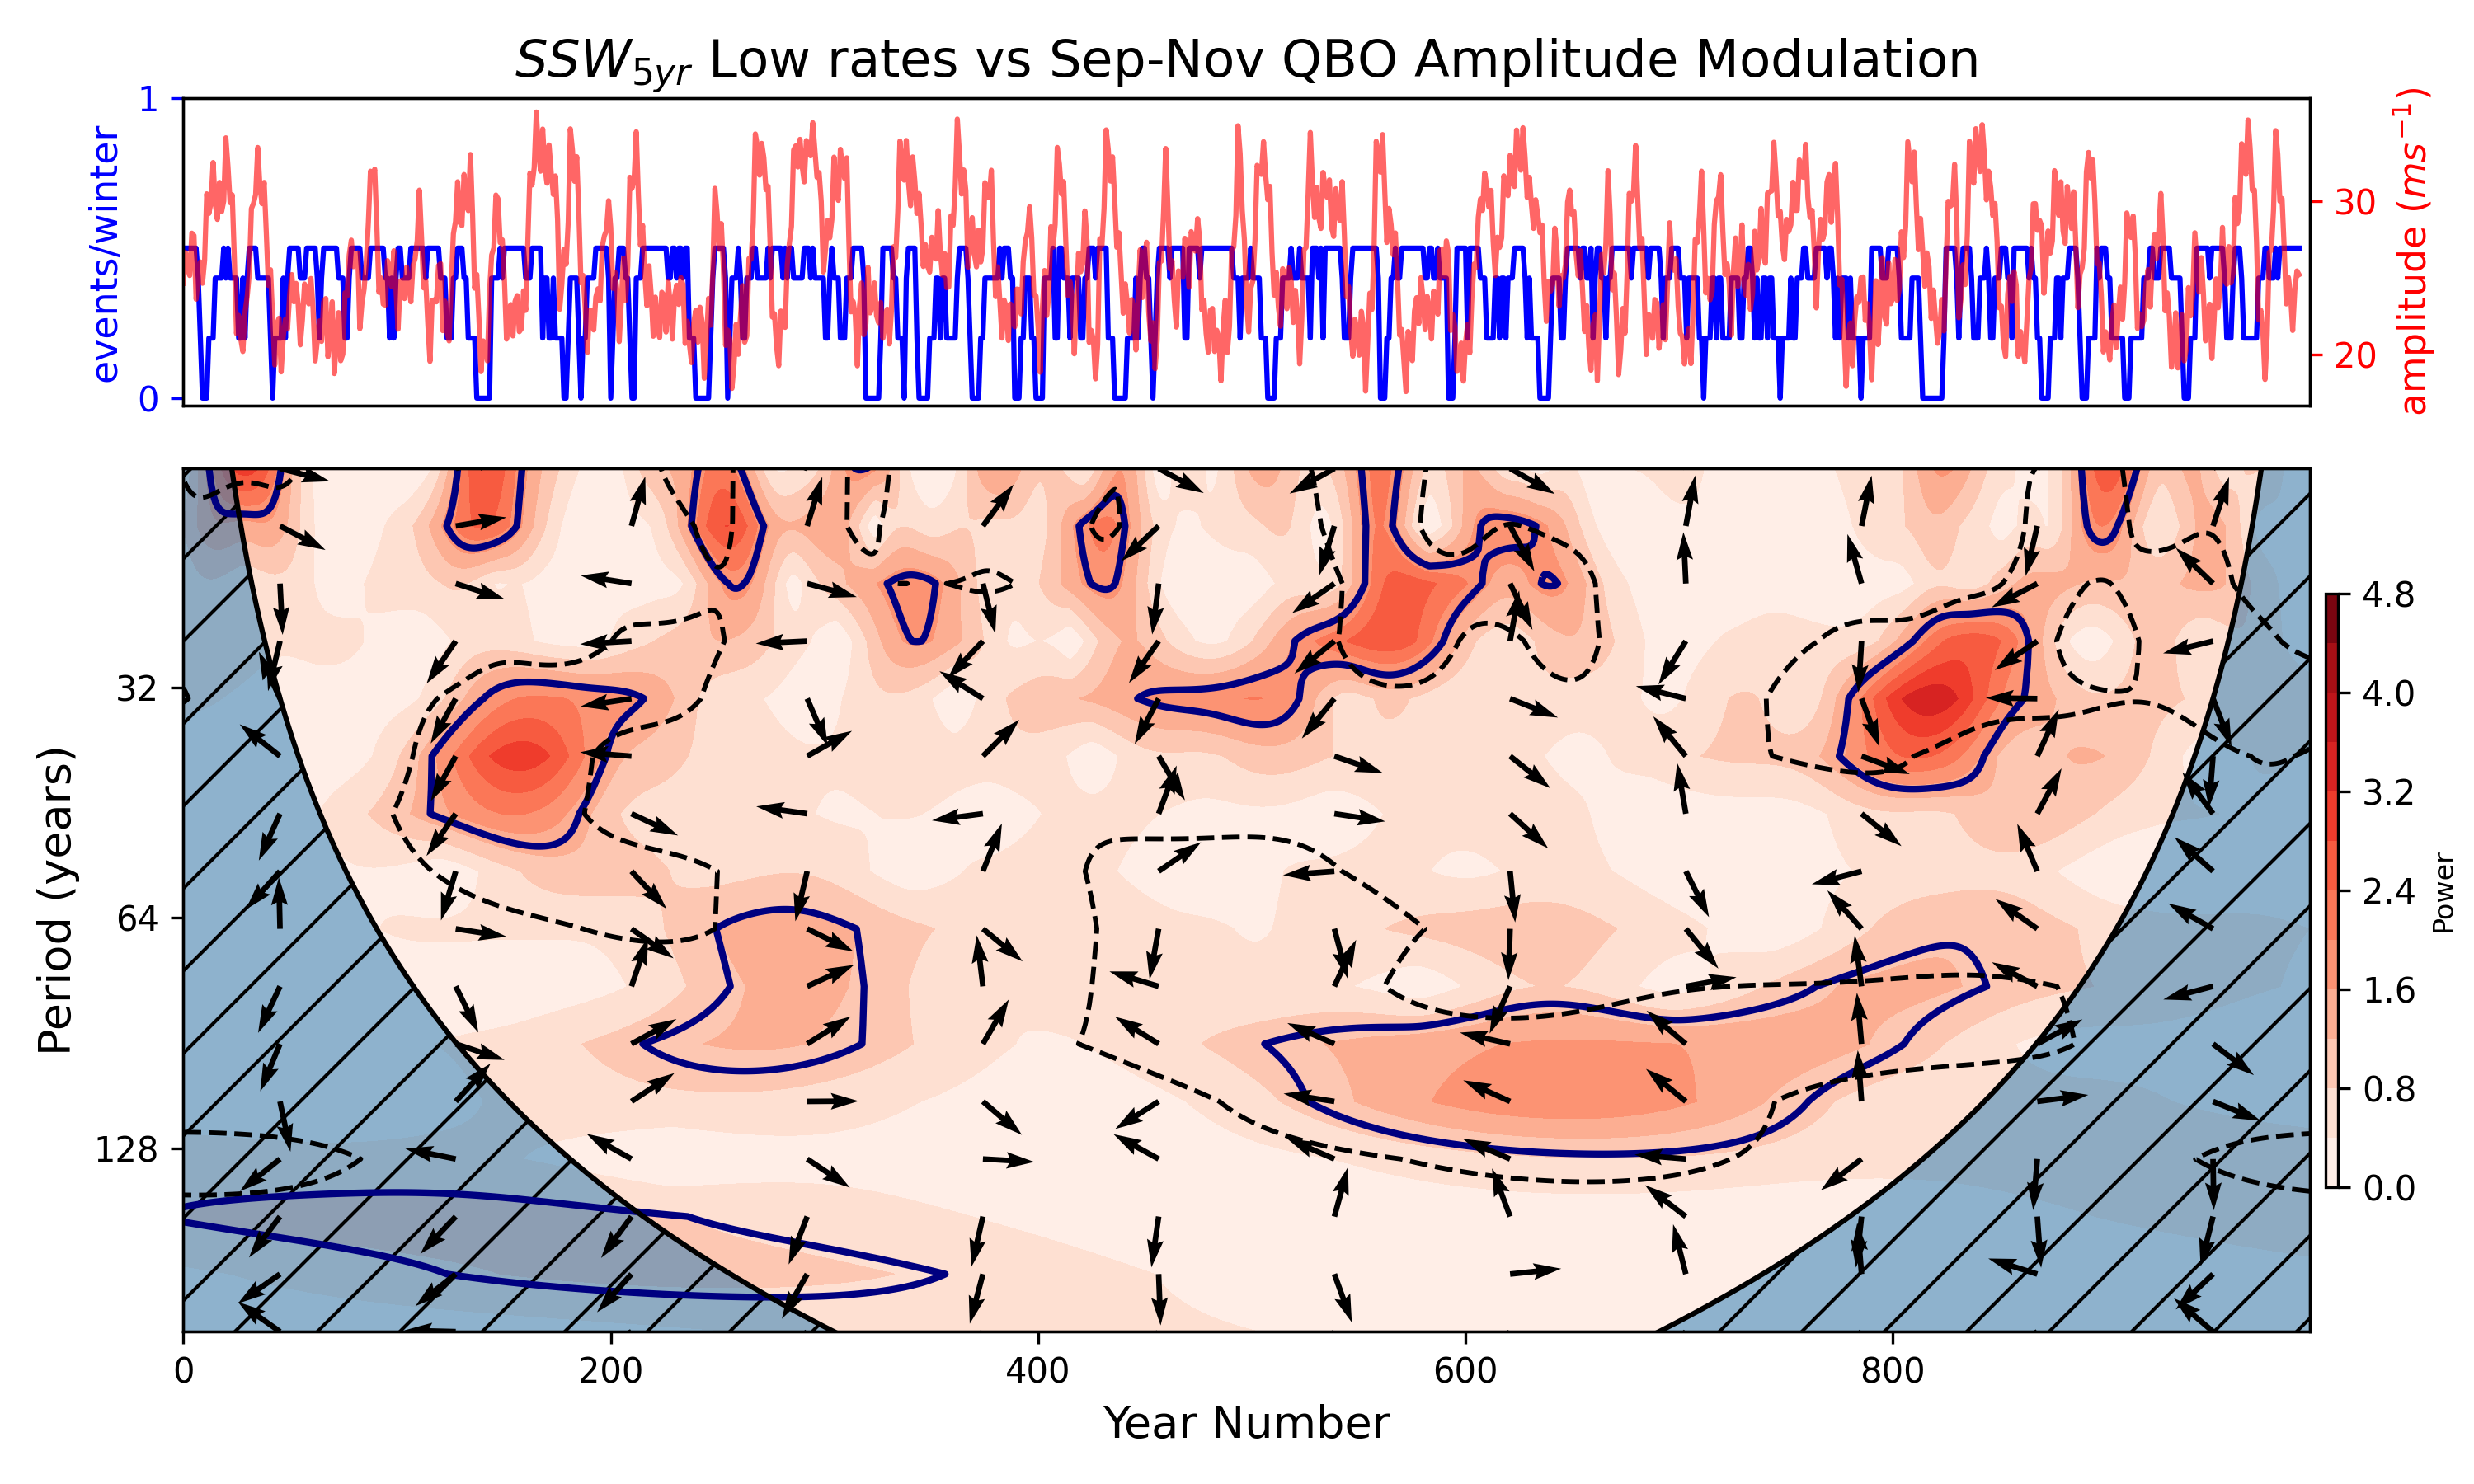
\includegraphics[width = 0.8\linewidth]{Figures/Figures-background/cross_power_SSWs_lowrate_vs_QBO_amplitude_modulation_5yr_mean.png}
\caption[cross power spectrum between deep QBO amplitude and SSW$_{5yr}$ with variations in high SSW rates removed]{\textbf{Top}: $SSW_{5yr}$ time series with variability in high SSW rate intervals removed by setting all rates above the climatological mean (0.54 events per season) to the mean (blue) and Sep-Nov deep QBO Hilbert Amplitude index smoothed with a 5 year window (red). \textbf{Bottom}: Cross wavelet power spectrum between the two time series.}
\label{fig:SSW_low_rate_QBO}
\end{center}
\end{figure}

An obvious question is whether this sensitivity to deep QBO westerlies that we find in the model is also present in the real atmosphere. Examination of the ERA-Interim dataset shows limited support. Some winters in the 1990s are characterised by anomalously westerly Sep-Nov equatorial winds which are vertically coherent between the 15 and 30\,hPa levels. However this effect is intermittent and does not span the whole interval of the 1990s during which SSWs were markedly absent in the observational record (not shown). On the other hand, a mini hiatus that was present in the mid 2010s is associated with 3 years of deep westerly anomaly in the QBO. Overall, it is clear that the relationship, if present in the real atmosphere, is likely obscured by other factors including greenhouse gas increases and volcanic eruptions and the observational dataset is too short to provide useful validation for these long timescale variations.  

\section{Summary and Discussion}
While there is much observational evidence for an impact of SSWs on the underlying tropospheric weather and climate, their multi-decadal variability and the associated forcing mechanisms are not well understood due to the short observational record. Analysis of long climate model simulations is currently the only available tool for understanding this variability. In this chapter we have examined variability in the appearance of hiatus and intervals of consecutive SSWs in a 1000-yr pre-industrial control simulation of one such model (UKESM).

We found realistic decadal and multi-decadal variability in the model, with hiatus intervals of 10 years or more in which no SSWs occurred, similar to the observed SSW record in the 1990s \citep{pawsonCold1999b, Shindell1999} and also intervals of consecutive-event periods in which at least one SSW occurred every year, as observed in the early 2000s \citep{manneyRemarkable2005a}. A 5-yr smoothed representation of SSW frequency ($SSW_{5yr}$) was found to vary periodically for approximately 450 years of the 1000-yr simulation with maxima in wavelet power corresponding to periodicity of around 60-90 years. 
A possible tropical SST source of this long-term variability was investigated. Wavelet and cross-spectrum analyses were performed using a variety of different tropical SST indices, including the ENSO 3.4 index, and also an index of the strength of the Aleutian Low (AL) which is linked to large-scale planetary wave forcing of the winter stratosphere. While all of these indices displayed elements of long-term variability, some of which overlapped with the periodicity and time intervals seen in the $SSW_{5yr}$ spectrum, none of them could fully account for the extended 450 year interval of significant power at 60-90 years seen in the $SSW_{5yr}$ spectrum. The weak relationship between the AL and SSW occurrence is unexpected and modifying the metric by using a box average SLP measure utilised in \cite{garfinkelWhy2012b} did not recover a stronger connection. Further analysis of the AL-SSW relationship in the simulation would be useful to explore whether the AL exhibits a connection with the NH winter mean vortex winds or other continuous vortex metrics such as the NAM even though there is no apparent connection with SSW occurrence. 

A second possible source of long-term variability involving variations in the QBO was also investigated. A range of QBO indices were considered, including the standard approach of using equatorial winds at a specified pressure level e.g. 50 hPa and also a 'deep QBO' index which takes the average QBO wind over 15-30 hPa, designed to capture the degree of vertical coherence in the QBO winds (following \cite{graySurface2018b} and \cite{andrewsObserved2019d}). A straightforward wavelet analysis of these QBO indices reveals no power at periodicity longer than 2-4 years. However, while there is evidently no long-term variability in the frequency of the QBO, visual examination of the QBO time series clearly shows the presence of long-term variability in the QBO amplitudes. A measure of this amplitude modulation was extracted by taking the Hilbert Transform of the QBO index. Wavelet analysis of the amplitude variations from the Hilbert Transform of the QBO indices showed long-term periodicity matching that seen in the $SSW_{5yr}$ wavelet analysis. In particular, the deep QBO index exhibited significant signals coincident with those in $SSW_{5yr}$ corresponding to periodicities of around 90 years. This overlap accounted for nearly all 450 years of SSW variability present on the 90 year timescale. Regression analysis of 5 year smoothed and filtered indices confirmed the contribution of the deep QBO amplitude to variability in SSWs on timescales greater than 60 years. 

Our analysis has therefore revealed an unexpected relationship between the strength and vertical coherence of the QBO and long-term variability in the frequency of SSWs. The relationship was found to be particularly sensitive to the QBO westerly phase. Extended periods of deep westerly QBO phases were associated with hiatus periods with few or no SSWs, consistent with the Holton Tan relationship. While this result appears compelling, it should be noted that the model showed some biases in its QBO associated with the period and descent rate of shear zones. The extended period of close to 3 years could introduce an element of phase locking between the QBO and seasonal cycle causing winter months to occur preferentially in one QBO phase over the other (evident from figure \ref{fig:SSW_hist_QBO_phase}, legends). This may influence QBO-vortex coupling. However, these biases are common in modern GCMs \citep{bushellEvaluation2020b} and \cite{raoModulation2019d} show UKESM's representation of the HT effect is better than most major GCMs submitted to CMIP6 indicating this pi-control remains one of the most effective tools for studying multi-decadal variability in the stratosphere. 
%Recent work has also shown a large degree of inter-model variability exists in representations of the QBO as well as SSWs \citep{bushellEvaluation2020b, ayarzaguenaUncertainty2020b} so it is possible the result from this study is model dependant. Additional analysis of long simulations from different models is required to verify these results. 


Combining the results of all these analyses, our overall conclusion is that multi-decadal variability in SSW frequency in UKESM is primarily accounted for by long term variability in QBO-SSW coupling, particularly at periodicities of around 90 years and, to a lesser extent, by variability in the intensity of the Aleutian Low at periodicities around 60 years, although coherence with the AL signals is far less persistent than with the QBO. Given the observed impact of SSWs on the underlying tropospheric weather and climate, improved understanding of the source and mechanisms of long-term variability in QBO-SSW interactions is likely to help improve future seasonal weather forecasts and decadal-scale climate predictions.

\subsection*{Outlook}
\label{sec:outlook_origins}
While the results from this chapter provide a novel type of variability in SSWs and its possible origin, the work reveals a number of areas of further research which we aim to address in subsequent chapters of this thesis.

\paragraph{Surface influence of SSW signals:} While we suggest a set of drivers for periodic signals in SSWs, we do not assess the influence of signals in hiatuses on the surface. Of particular interest may be the NH Ocean basins given the timescales of signals considered in this study (similar to characteristic modes of variation such as the AMOC and AMV) as well as vortex variability's association with surface modes in this region \citep{baldwinStratospheric2001a}. Analysis in the following chapter examines the interaction between signals in a vortex timeseries and key modes of tropospheric, surface and Atlantic variability.

\paragraph{Origins of QBO amplitude modulations:} Open questions also remain regarding the role of signals in SSW time series in the earth system. If, as we propose here, amplitude modulation in a deep QBO metric is responsible for driving SSW signals, a natural area of further research could focus on understanding the cause of such amplitude variability. Categorising whether QBO signals are externally driven by features such as tropical upwelling, ENSO (as well as other tropical SST variability) and deep convection or internally generated within the stratosphere would likely be key for this understanding. Work in chapter 4 also includes a closer analysis of tropical upwelling and deep convection in the Pacific region to attempt to diagnose the source of QBO amplitude modulation fully.

\paragraph{The role of QBO vertical structure in teleconnections:} Finally, the precise nature of QBO-SSW interactions is still not fully understood \citep{ansteyHighlatitude2014b}. While the importance of wave-mean flow interactions is widely recognised, further analysis is required to explore the relevance and usefulness of the deep QBO index highlighted in this chapter, that identifies a vertically coherent QBO phase. It appears to be especially relevant to long-term QBO-SSW interactions during the QBO-W phase and its importance is suggested in recent work \citep{andrewsObserved2019d}. Findings from a set of GCM experiments designed to explicitly analyse the role vertical QBO structure in teleconnections are presented in chapter 5. 

\chapter{Interactions between the Stratospheric Polar Vortex and Atlantic circulation} 
\begin{quotation}
  Much of the work contained in this chapter is based upon xxx,
  published in \emph{Journal of Climate}.
\end{quotation}

\label{cha:surface}

\section{Introduction}
Chapter 3 demonstrated that the appearance of SSWs varies on multi-decadal timescales in a pi-control simulation. Given the well studied downward influence of vortex variations over the Atlantic sector (see section \ref{sec:Downward_influence}), a natural question that follows from this finding is to what extent do these multidecadal signals influence modes in tropospheric and surface climate? The majority of studies that have examined the associations between the stratospheric polar vortex and surface anomalies have considered their in-season impact, however the Atlantic region exhibits key modes of multi-decadal variation in ocean circulation and SSTs (the AMOC and the AMV, section \ref{sec:multi-decadal_background}) which are in turn key drivers of climate variation. In this chapter, we assess the influence of vortex anomalies on surface and Ocean variations across multiple timescales (in-season to multi-decadal)
in the same pi-control simulation as analysed in chapter 3. We also utilise the relationship between the vortex and AMOC established in this model to estimate the contribution of the stratosphere, namely the 8 year SSW hiatus interval in the 1990s, to recent trends in AMOC observations.

The effect of decadal to multi-decadal scale variation in the vortex on the surface has been considered in previous works, but its true nature is not fully understood. \cite{manziniStratospheretroposphere2012} examines decadal fluctuations in SSW events in a 260 year prescribed SST simulation of a GCM and analyse impacts of these signals at the surface. They show that decadal vortex variability excites similar timescale variations in surface temperature and sea ice coverage between Greenland and Norway over the Atlantic sector. They propose this connection to be indicative of a delayed response of the AMOC to stratospheric forcing via the NAO which  subsequently influences northward Atlantic heat transfer and sea ice melt rates as well as surface temperatures anomalies. \cite{haaseImportance2018} analyse the in-season impact of SSW events on the strength of deep convection in the North Atlantic that occurs through the impact of SSWs on the NAO using a model (CESM1 WACCM). The study notes the presence of an anomalously shallow  mixed layer depth in the Labrador Sea following an SSW event. 

An association between stratospheric polar vortex variability and the AMOC on decadal timescales has also been previously investigated \citep{reichlerStratospheric2012, Schimanke2011} but the mechanism of its influence remains unclear. For example, \cite{reichlerStratospheric2012} examine the response of the AMOC to strong and weak polar vortex events and show a lagged response in the AMOC leading to oscillatory responses. They propose a pathway involving alterations of wind stress and ocean-atmosphere heat flux anomalies in the West Atlantic due to the changed NAO patterns following the vortex events. The effect is seen in both reanalysis and to some extent in a suite of CMIP5 models. An impact of long-term changes in the NAO on the strength of the AMOC is supported by a number of studies \citep{visbeckOcean1998, delworthImplications2000, delworthMultidecadal2000, edenMechanism2001}. Most recently \cite{delworthImpact2016} used a set of idealised GCM experiments in which they impose a perpetual ocean-atmosphere heat flux pattern associated with different NAO phases. They find significantly different AMOC mean states depending on the imposed pattern (a stronger AMOC under positive NAO flux conditions than a control simulation). 


\section{Data And Methods}
\subsection{Model Configuration and Observation Data}

We analyse output from the same GCM simulation as presented in chapter 3 - the pi-control simulation of UKESM (see section \ref{sec:model_config}). As in chapter 3, we choose the pi-control due to the length of integration relative to the timescales we wish to consider and to analyse the internal variability of the system in this model. 

To estimate the contribution of stratospheric variations to recent observed AMOC trends we also make use of observation based datasets of the atmosphere and oceans. First, we utilise the reanalysis data from the European Centre for Medium-Range Weather Forecasts (ECMWF): ERA5 \citep{hersbachERA52020} for observation based geopotential height (GPH) fields. Similar to its predecessor, ERA-Interim (section \ref{sec:ERA_data}), ERA5 consists of a set of observations assimilated through 4D-var using ECMWF Integrated Forecast System (IFS). However, ERA5 utilises the latest version of the IFS which operates at a greater horizontal grid resolution to ERA-Interim (31km vs 80km) as well as a higher vertical resolution and maximum height (60 levels up to 10hPa vs 137 levels to 1 hPa) \citep{hersbachERA52020}. Most relevant for stratospheric representation is the inclusion of an improved gravity wave parameterisation scheme in the latest IFS and the latest IFS exhibits a marginal improvement in the predictability of SSW events compared to its predecessors \citep{orrImproved2010}. Despite these improvements in the underlying model, \cite{hersbachERA52020} reports no significant improvement in stratospheric representation between ERA5 and ERA-Interim due to a combination of IFS model bias in the middle to upper stratosphere and sparse observations in the same region. We choose to utilise ERA5 as opposed to ERA-Interim for analysis in this chapter as we consider observations of the AMOC and the vortex up to near present day. ERA5 provides data up till present day while ERA-Interim has been discontinued as of 2019 so ERA5 is a preferable dataset in this case. 

Second, we use the Rapid Array Dataset which provides time-depth profiles for the meridional overturning mass streamfunction in the Atlantic region at 26$^{\circ}$N \citep{moatAtlantic2020}. These data are measured through a combination of ocean mooring, ship based, satellite and submarine telephone cable observations to estimate the strength of primary contributions to the meridional overturning circulation: Ekman transport (through wind stress), transport through the Florida Straits and transport driven by EW density gradients between the American and African continents \citep{mccarthyMeasuring2015}.

\subsection{Model Diagnostics}
\label{sec:model_diagnostics_surface}
We utilise the Northern Annular Mode (NAM) as a metric for the strength of the vortex as used by \cite{baldwinStratospheric2001a} as well as numerous subsequent studies. The NAM is defined as the 1st principle component of the zonal mean, deseasonalised geopotential height field evaluated at latitudes north of $20^{\circ}N$ over the NH winter season (Nov-Mar) on a given pressure level. To measure the vortex strength we evaluate the NAM on a level in close proximity to the vortex edge, 10hPa, and the resulting index is henceforth known as NAM$_{10}$. We choose to utilise a continuous vortex metric for this work as opposed to the event based measured used in chapter 3 as the NAM captures both types of anomalous vortex behaviour (strong and weak). Cross spectral analysis of the SSW time-series and the QBO (figure \ref{fig:SSW_low_rate_QBO}) suggested an important role of SSW hiatuses in multi-decadal modes of variation. As a result, a continuous metric that distinguishes between a weak, strong and neutral vortex is highly useful for this analysis. An individual vortex event (either strong or weak) is recorded when the daily NAM$_{10}$ crosses +1.5 (strong) or -2 (weak). The day on which this reversal occurs is referred to as the central date. After this date, the NAM$_10$ must recover to neutral (between -2 and 1.5) for a period of at least 10 consecutive days (which is the approximate radiative timescale of the mid-stratosphere) before another event can be recorded. The strong threshold value for events is chosen in accordance with the methodology of \cite{baldwinStratospheric2001a} and the weak threshold selected such that it results in approximately the same rate of weak events (SSWs) as is reported in chapter 3 (figure \ref{fig:SSW_histogram}) using the same simulation of UKESM but with a zonal wind definition of SSWs (0.54 events/winter).

We also use the NAM$_{10}$ to derive an index for the appearance of intervals of consecutive winters which show persistent vortex behaviour. The persistent NAM$_{10}$ interval index is defined as the annual mean Nov-Mar NAM$_{10}$ (which gives a measure of vortex strength for each winter) which has additionally been smoothed using a Gaussian filter. This smoothing is carried out through a convolution of the time-series with a 1D Gaussian kernel in the time domain given by

\begin{equation} \label{Gaussian_filter}
f(t, \sigma) = \frac{1}{\sqrt{2 \pi \sigma^2}} e^{-\frac{1}{2}\big(\frac{t}{\sigma}\big)^2}
\end{equation}

Where $\sigma$ is the standard deviation of the distribution defined by the kernel. We choose $\sigma$ = 2 years following the method of \cite{reichlerStratospheric2012} and as a method analogous to the 5 year smoothing applied to an SSW timeseries in chapter 3. The selection of $\sigma = 2$ years allows contributions to the smoothed value from values approximately 7 years either side of the central year as the value of the Gaussian window decays to near 0 approximately $3.5\sigma$ from its mean. However the largest contributions come from 3-4 years either side of the central year. This allows the smoothing to capture instances of $\sim$6-8 consecutive years with persistent vortex behaviour, a similar length to intervals observed in reanalysis (e.g. the 1990s, \cite{pawsonCold1999}). We subsequently define persistent NAM$_{10}$ intervals, when the vortex exhibits the same type of behaviour for a number of consecutive years, using extreme values of the smoothed NAM$_{10}$ index. A persistent NAM$_{10}$ interval is recorded when the smoothed NAM$_{10}$ index value falls within the top 5 percentile values. Once such an interval occurs, another cannot be recorded for 15 years after to avoid choosing multiple central years within the same interval. Using 5 percentile values gives approximately the same rate of persistent vortex intervals as is reported in \cite{reichlerStratospheric2012} so we proceed with this threshold throughout for a direct comparison with this study. Tests were also carried out to assess the sensitivity of our results to this threshold and are reported in section 3.

We define an AMOC index following the procedure in \cite{reichlerStratospheric2012}. The AMOC is defined using overturning streamfunction field averaged in the Atlantic sector. At each time point the AMOC index is the maximum streamfunction value at any depth at a chosen latitude. We evaluate the index at 30N, 45N and 50N and measure the response and co-variability with the SSW timeseries and other climate indices defined below. We derive the observed AMOC index from the Rapid Array data as the maximum MOC at each time point at 26N. We also utilise a definition of the North Atlantic Oscillation from \cite{hurrellNorth2003}. The NAO index is defined as the 1st principle component (PC) of the Dec-Mar MSLP in the region $20^{\circ}-80^{\circ}N, 90^{\circ}W-40^{\circ}E$. The pc is calculated by taking the first empirical orthogonal function (EOF) of deseasonalised MSLP anomalies and projecting this EOF onto the anomaly field. We additionally derive an Ocean-Atmosphere heat flux field defined as the sum of latent and sensible heat fluxes between the ocean surface and the atmosphere (i.e. positive values indicate exchange of heat from the ocean to the atmosphere). We derive an index for the occurrence of deep convection anomalies in the equatorial eastern Pacific region. This index is defined by the top of atmosphere outgoing longwave radiation (OLR) averaged over the box 10$^{\circ}$\,S–10$^{\circ}$\,N, 240$^{\circ}$\,–290$^{\circ}$\,E. The OLR field is utilised as it acts as a proxy for the occurrence of convection anomalies - When deep convection is enhanced, cloud top height is increased and therefore OLR is reduced. The East Pacific box is selected following a sensitivity analysis to establish the region which exhibits 90 year timescales variations in OLR. It is also a similar region to studies which consider east pacific ENSO patterns which is identified as a separate mode of variability to the traditionally used central pacific ENSO region \citep{johnsonHow2013}.

Finally, we utilise the same QBO metric as in the wavelet analysis of chapter 3 (see section \ref{sec:model_diagnostics}. This is defined as the Zonal Mean Zonal Wind (ZMZW) averaged over the latitude range 5$^{\circ}$\,S–5$^{\circ}$\,N,  and the pressure level range 15-30hPa. As with chapter 3 we also consider the Hilbert amplitude of the deep QBO as an instantaneous amplitude metric (see equations \ref{eq:hilbert1}-\ref{eq:hilbert3}). 

\section{In-season surface responses to anomalous vortex events}
We begin by diagnosing the in-season response to anomalous vortex events exhibited by surface variability in the model to assess its suitability for studying interactions on longer timescales. Figure \ref{fig:surface_comp_all} shows the mean sea level pressure (MSLP) composite differences between strong and weak polar vortex years (figure \ref{fig:surface_comp_all}, top row). The composites have been determined by selecting MSLP values associated with events in which the daily NAM$_{10}$ values cross +1.5 (strong) or -2 (weak) (see section \ref{sec:model_diagnostics_surface}). The composite differences demonstrate a significant lagged MSLP response, with strong (weak) vortex years  corresponding to a positive (negative) NAO pattern, in agreement with previous model and observational studies (see section \ref{sec:Downward_influence}). The NAO anomalies peak in magnitude at a lag of 1-2 months following the vortex anomalies with significant anomalies still visible for up to 3 months. There is also a weak positive NAO pattern that leads the vortex anomalies by up to one month ($-1 - 0$ month lags). This may be an indication that an anomalous NAO pattern is a precursor for an anomalous vortex, or it could be a response to the initiation of the vortex anomaly since this usually commences in the upper stratosphere and pre-dates the event's central date defined at 10 hPa. Further exploration of this weak NAO signal is outside the scope of the analysis presented here. Additionally, a much stronger significant positive anomaly over the Aleutian low (AL) region is evident in the month leading up to the vortex anomaly. This signal has been widely studied \citep{raoModulation2019a} and links the intensity of the AL to the strength of vertically propagating planetary waves that subsequently interact with the stratospheric vortex and influence its strength (section \ref{sec:external_influence_AL}). Analysis in chapter 3 examined this coupling using the same pi-control simulation as presented here and found a similar statistically significant relationship between the AL and the frequency of SSWs but the regression coefficients were small in comparison with the QBO influence. Here the association between the AL and the vortex strength appears marginally stronger (r = 0.39 with the NAM$_{10}$) which may be due to the NAM's ability to capture both types of vortex anomalies (strong and weak). In chapter 3 we also showed that the AL exhibited minimal decadal to multi-decadal variability that was coherent with the decadal to multi-decadal variability of the vortex (\ref{fig:AL_wavelet} and for this reason the role of the AL is not considered in detail in this chapter.

\begin{center}
\begin{figure}[h!]
\noindent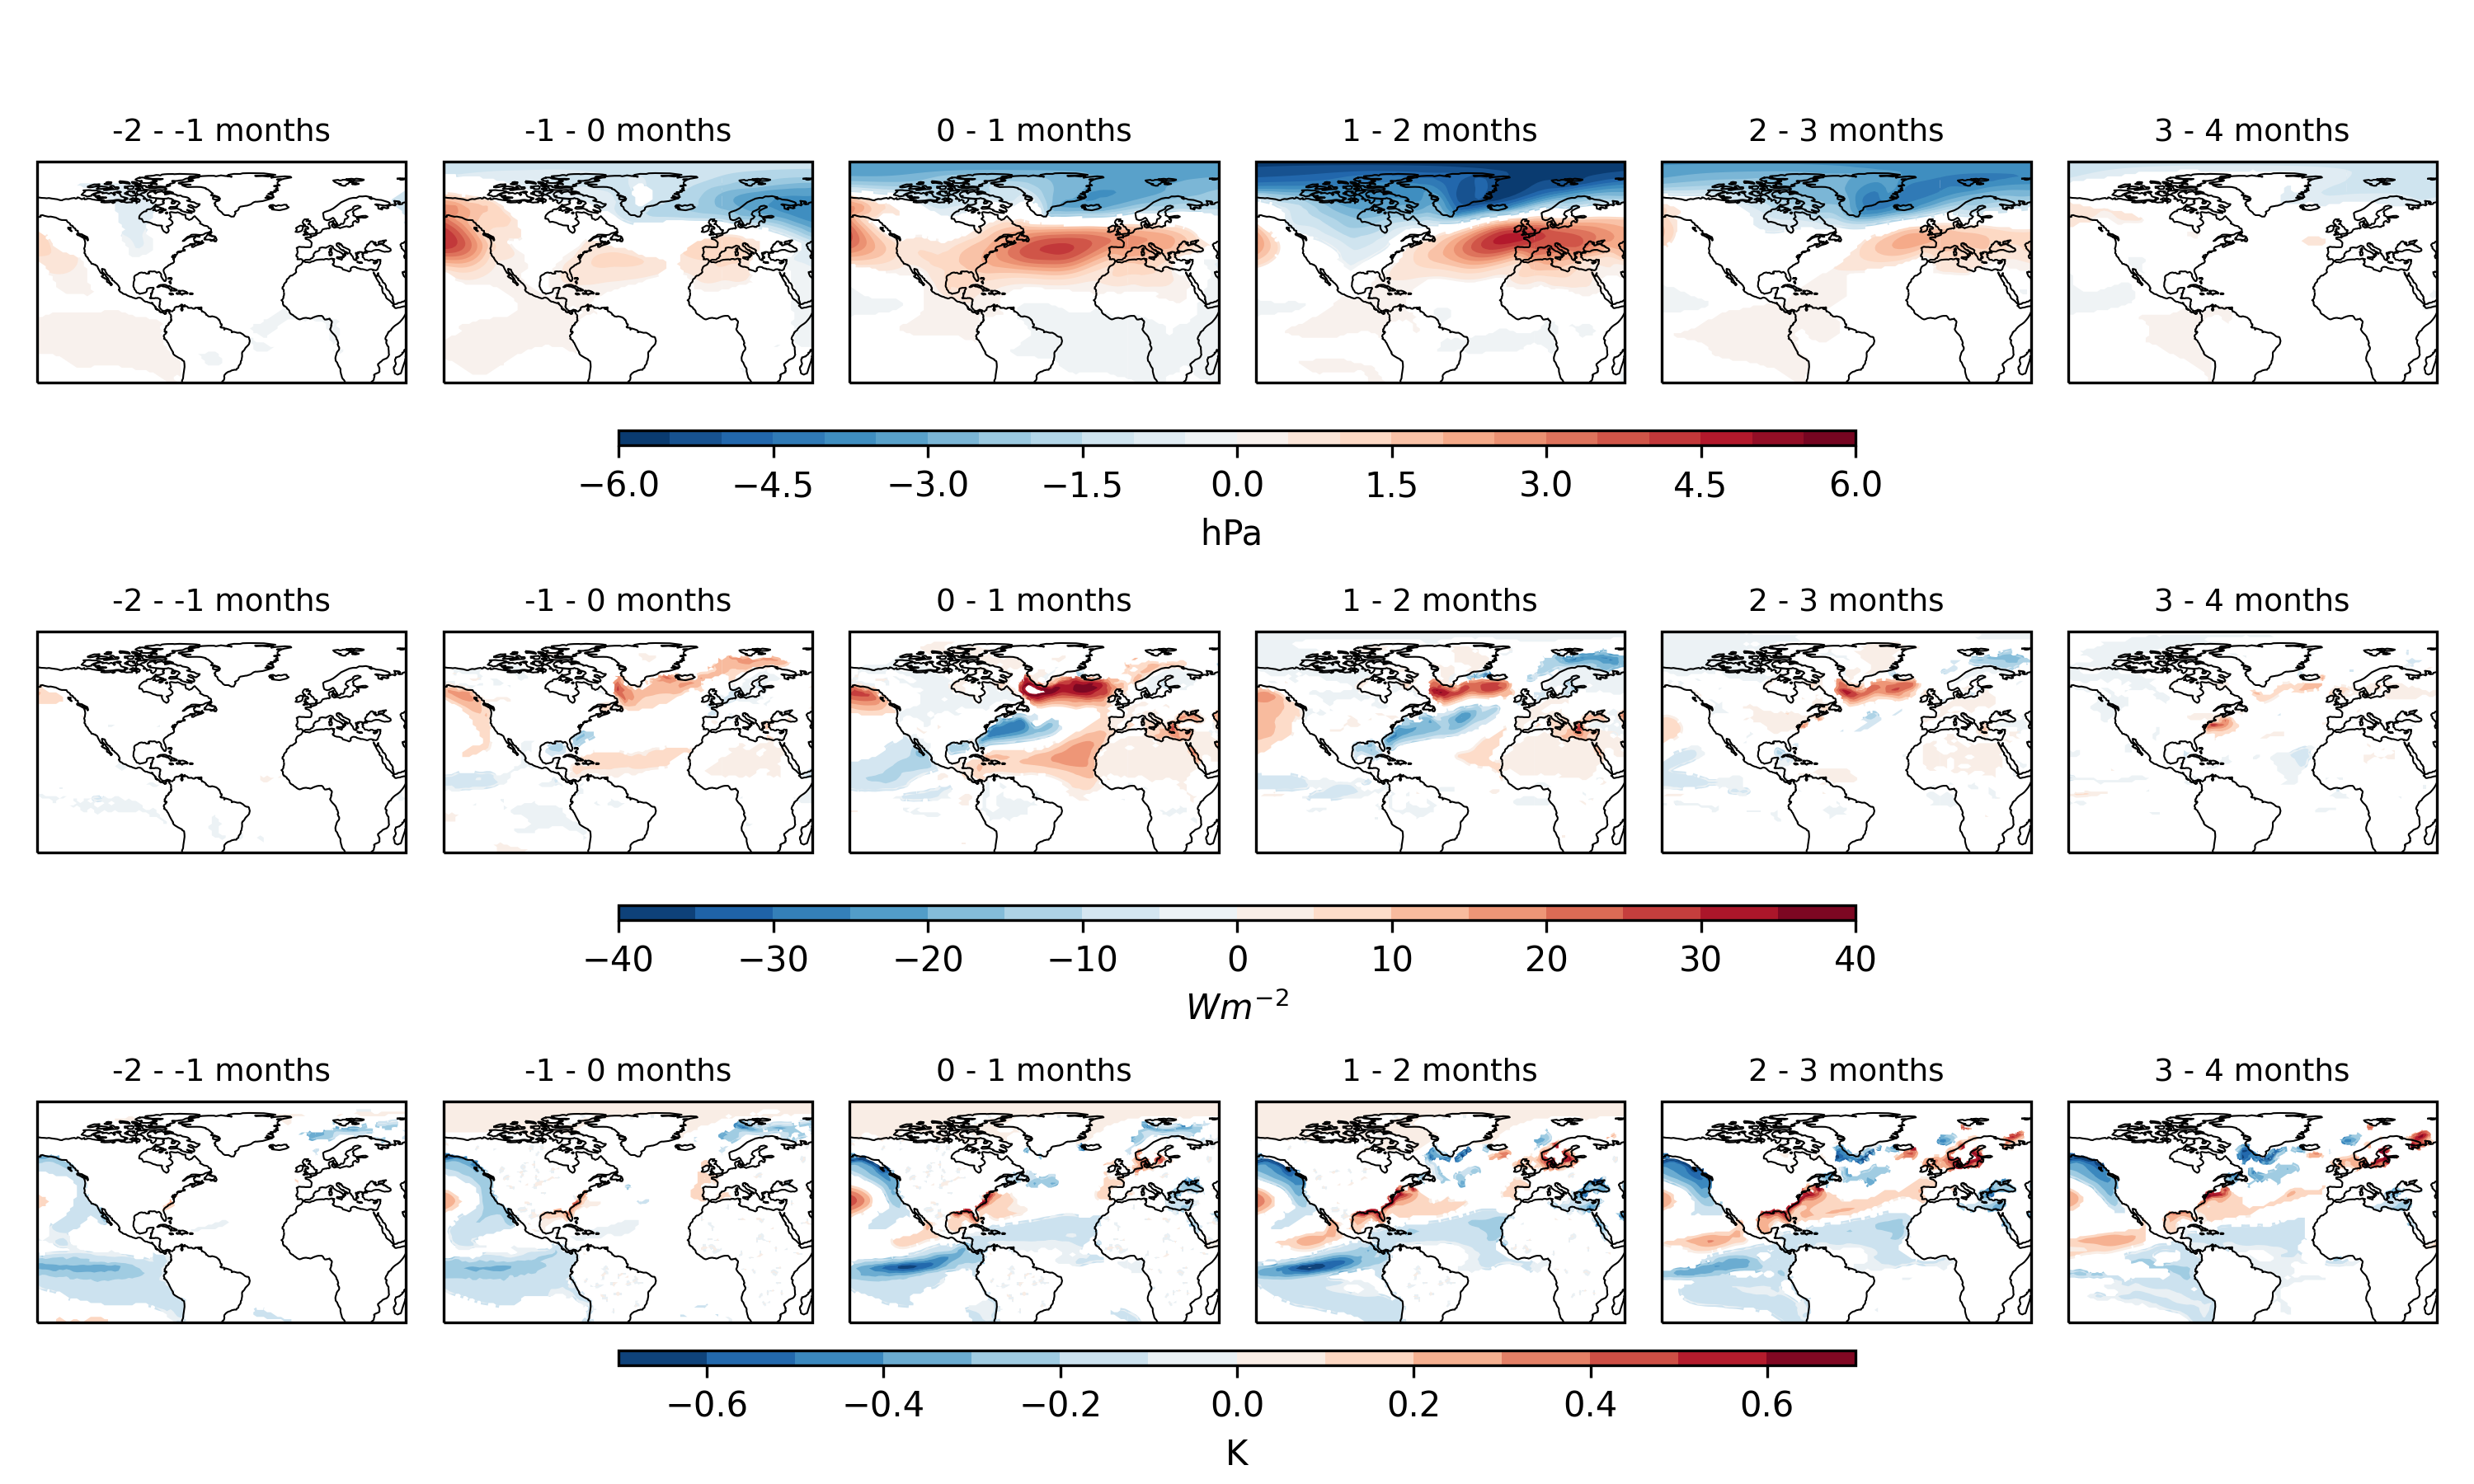
\includegraphics[width = \linewidth]{Figures/Figures-surface/in_season_response_NAM_combined.png}
\caption{Surface patterns associated with anomalous winter stratospheric NAM$_{10}$ events. \textbf{Top row}: Monthly mean sea level pressure anomaly, \textbf{middle row}: Ocean-Atmosphere heat flux defined as the sum of latent and sensible heat fluxes and \textbf{bottom row}: SSTs. Coloured shading shows where the composite differences between strong and weak NAM$_{10}$ events are statistically significant at the 95\% level under a 2 tailed students t-test. The title of each sub-figure indicates the month range relative to the central date of each NAM$_{10}$ anomaly. Signals at negative times indicate that the surface anomaly leads the stratospheric NAM$_{10}$ anomaly. Signals at positive  times indicate that the stratospheric NAM$_{10}$ anomaly leads the surface response.}
\label{fig:surface_comp_all}
\end{figure}
\end{center}

The model also exhibits significant responses in ocean-atmosphere heat flux (figure \ref{fig:surface_comp_all}, middle row). The largest flux anomalies are seen within 30 days (lag 0-1 month) and their spatial pattern resembles that of a North Atlantic tripole with positive anomalies over the Labrador sea and between Greenland and Western Europe, negative anomalies off the east coast of the USA and a second positive anomaly off the coast of north east Africa. This pattern is consistent with the model response found by \cite{reichlerStratospheric2012} to anomalous stratospheric NAM$_{10}$ events as well as the pattern associated with positive NAO phases in \cite{delworthImpact2016}. As with the MSLP composites, there are visible anomalies 30 days leading up to the identified events (lag -1 - 0 months) both over the North Atlantic and Pacific regions. The Atlantic pattern may correspond to early responses to a disrupted or strengthened vortex. The Pacific anomalies preceding events are considerably smaller than the Atlantic anomalies and are concentrated over the Aleutian low region.

The SST response to anomalous stratospheric NAM$_{10}$ events (figure \ref{fig:surface_comp_all}, bottom row) over the North Atlantic lags behind the heat flux anomalies by around 2 months, with the largest amplitude anomalies at around 2-4 month lags.  The anomaly pattern resembles that of the heat flux anomalies (with a change of sign), consistent with a mechanism in which the SSTs respond to the anomalous heat fluxes. A prominent negative tropical East Pacific anomaly is obvious in the months leading up to anomalous vortex events together with  anomalies that resemble the Pacific Decadal Oscillation (PDO) in the region of the Aleutian Low \cite{mantuaPacific1997} and these features persists for several months. Variability in this region is dominated by ENSO variations and a significant body of work has proposed teleconnections between ENSO and vortex strength, consistent with the type of association exhibited here (see section \ref{sec:external_influence_SSTs}), i.e. negative (positive) SSTs or la Ni\~{n}a (el Ni\~{n}o) conditions associated with an anomalously strong (weak) vortex. 

\section{Surface impacts of persistent vortex anomalies}
\label{persistent}
The in-season anomaly patterns associated with anomalous stratospheric NAM$_{10}$ events shown in figure \ref{fig:surface_comp_all} confirm that the model is able to reproduce the observed influence of vortex anomalies at the surface, particularly over the Atlantic region. We now extend the analysis to examine decadal-scale variability. Following the approach of \cite{reichlerStratospheric2012} we smooth the NAM$_{10}$ index  (figure \ref{NAM_and_filtered}) and then select the upper and lower 5 percentiles of this index to identify intervals with a persistent consecutive strong or weak polar vortex (see section \ref{sec:model_diagnostics_surface} for more details). The red and blue dots on figure \ref{NAM_and_filtered} indicate the central year of intervals identified with persistent consecutive vortex anomalies (each dot represents the centre of intervals of at approximately 8 years, see section \ref{sec:model_diagnostics_surface}). Characteristic surface responses associated with these intervals are then analysed by compiling composites of the relevant surface fields for the 80 years surrounding the central year of each positive and negative interval and calculating the (positive minus negative) composite difference. These can then be used to assess the potential surface impacts to observed intervals of persistent consecutive vortex anomalies, such as the consecutive strong anomalies throughout most of the 1990s and the consecutive weak anomalies in the early 2000s. 

\begin{figure}[h!]
\begin{center}
\noindent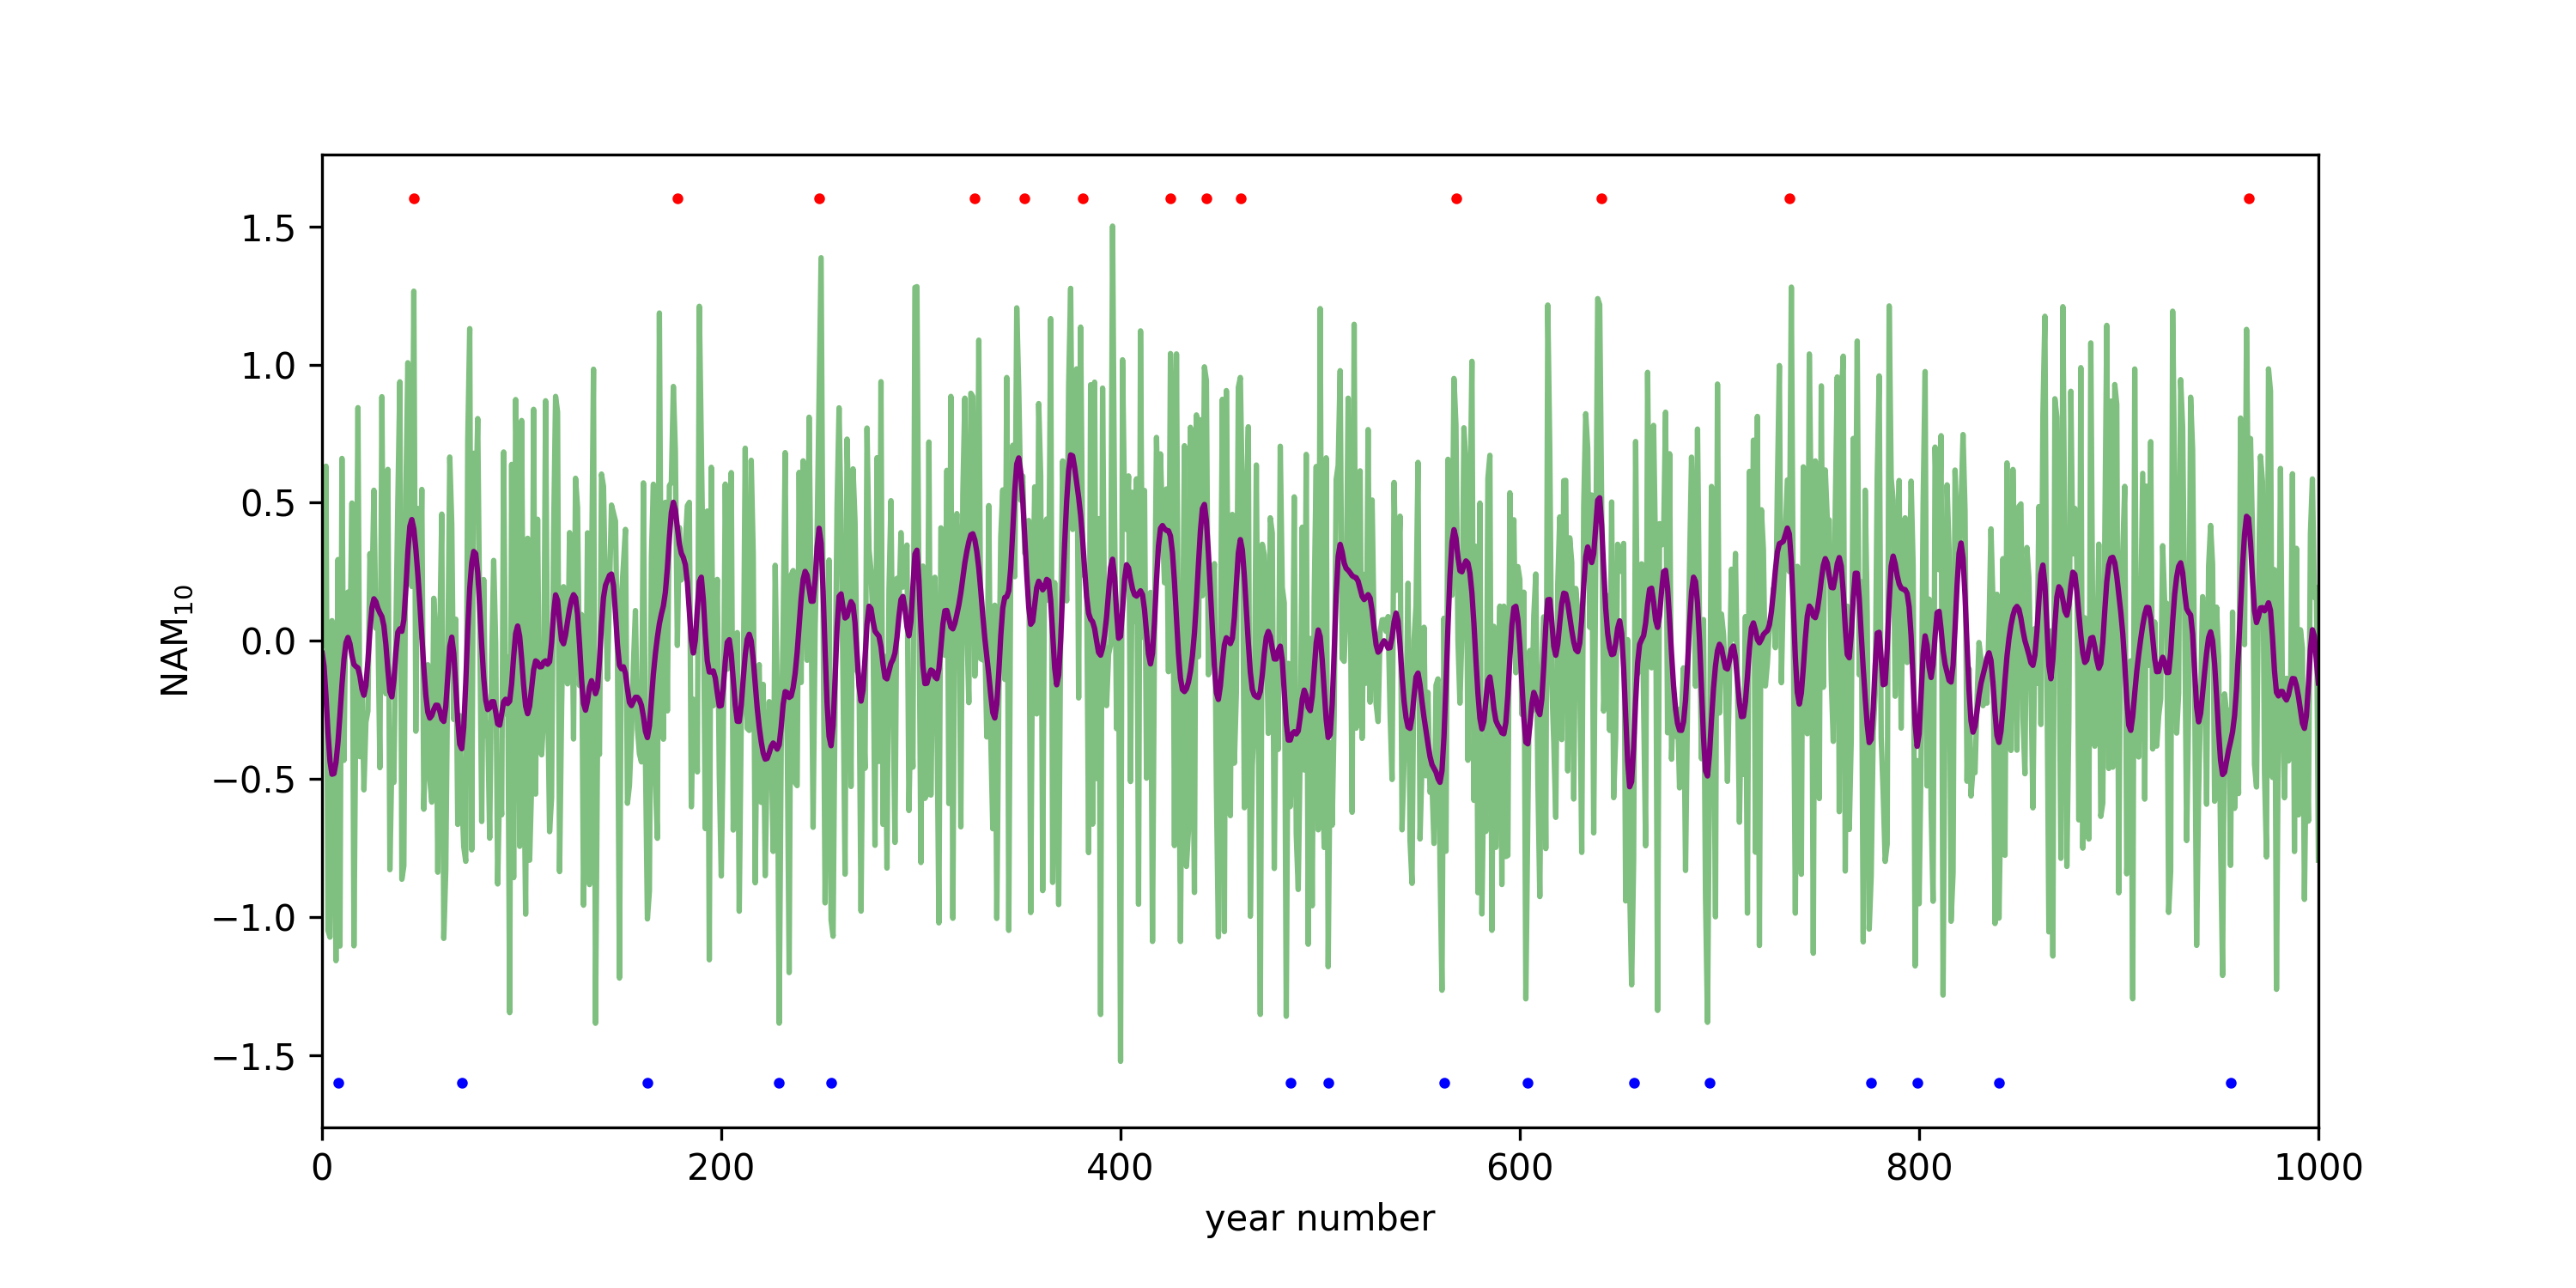
\includegraphics[width = \linewidth]{Figures/Figures-surface/NAM_and_filtered.png} 
\caption{Time series of the December-March mean NAM$_{10}$ index (green) level (\textbf{green}) and smoothed NAM$_{10}$ (purple) evaluated at the 10hPa. The smoothed series is calculated by applying a Gaussian filter ($\sigma = 2$ years) to the green series. Red and blue dots indicate the occurrence of persistent strong and weak vortex intervals respectively defined as extreme values (top and bottom 5 percentiles) in the filtered NAM$_{10}$ index. interval central years are selected such that at least 10 years lies between consecutive intervals.}
\label{NAM_and_filtered}
\end{center}
\end{figure}

A lead-lag analysis of composite differences in the AMOC strength at three different latitudes is shown in  figure \ref{AMOC_comp_NAM}. Positive lags indicate that the stratosphere leads the AMOC response, while negative lags indicate that the AMOC leads the stratospheric response. The figure can be directly compared with figure 4c of \cite{reichlerStratospheric2012}. As found by this work, an oscillatory AMOC response to the stratospheric anomalies is evident, with significant positive anomalies in the AMOC at 45N and 50N at lags of approximately 3-5 years after persistent NAM$_{10}$ intervals followed by negative anomalies at lags between 15 and 20 years. This response pattern is more clearly evident by taking the low pass filtered versions of the AMOC responses (figure \ref{AMOC_comp_NAM}b, d and f) in which we smooth the AMOC index with the same Gaussian filter used to construct the filtered NAM$_{10}$ index. Even after the high frequency signals have been removed, the composite differences still exhibit magnitudes up to 1.5Sv at 15-20 year lags and these are significant under a student's t-test. We note, however, that this low pass filtering of the AMOC time-series reduces the overall variance so that the threshold for a composite difference to pass the significance test is lower, and this may increase the responses that are deemed significant shown in figure \ref{AMOC_comp_NAM}. Nevertheless, given the large magnitude of the response in the filtered AMOC, we conclude that there is evidence of decadal scale variability in the NAM-AMOC interaction and the most significant responses occur when the stratosphere is leading the AMOC. This is in agreement with \cite{reichlerStratospheric2012} who suggest that decadal scale variability in vortex strength acts to amplify a similar timescale of variability in the AMOC through resonance of the two signals. Oscillatory response behaviour is not exhibited clearly by the AMOC at 30N, although negative anomalies at lags of 15-20 years after intervals are still visible. Response patterns at this latitude are also significantly smaller than those at 45N and 50N in the filtered composites (figure \ref{AMOC_comp_NAM}a and b). One possible explanation of this is that the coupling mechanism between the NAM$_{10}$ and AMOC may involve an AMOC response that originates at higher latitudes and then propagates equator-ward therefore exerting less forcing on the AMOC evaluated further south. \cite{zhangLatitudinal2010} also note latitudinal differences in the AMOC response so these differences between 30N, 45N and 50N are not unexpected. The AMOC signals at 45N and 50N also exhibit significant positive anomalies preceding the persistent vortex intervals, at a lead of approximately 20 years and this is also present, albeit smaller in magnitude, in the low pass filtered indices. This precursor to persistent NAM$_{10}$ intervals is not found in corresponding results from \cite{reichlerStratospheric2012} and the role of this feature is considered in more detail in section \ref{surface-strat_forcing}. Overall, these lead-lag difference analyses show that the NAM$_{10}$ and AMOC exhibit elements of co-variability and that decadal scale variations appear to be a key element to this teleconnection. Our results are broadly consistent with similar studies \citep{reichlerStratospheric2012} but with larger responses at lags of 10-20 years.

\begin{center}
\begin{figure}[h!]
\noindent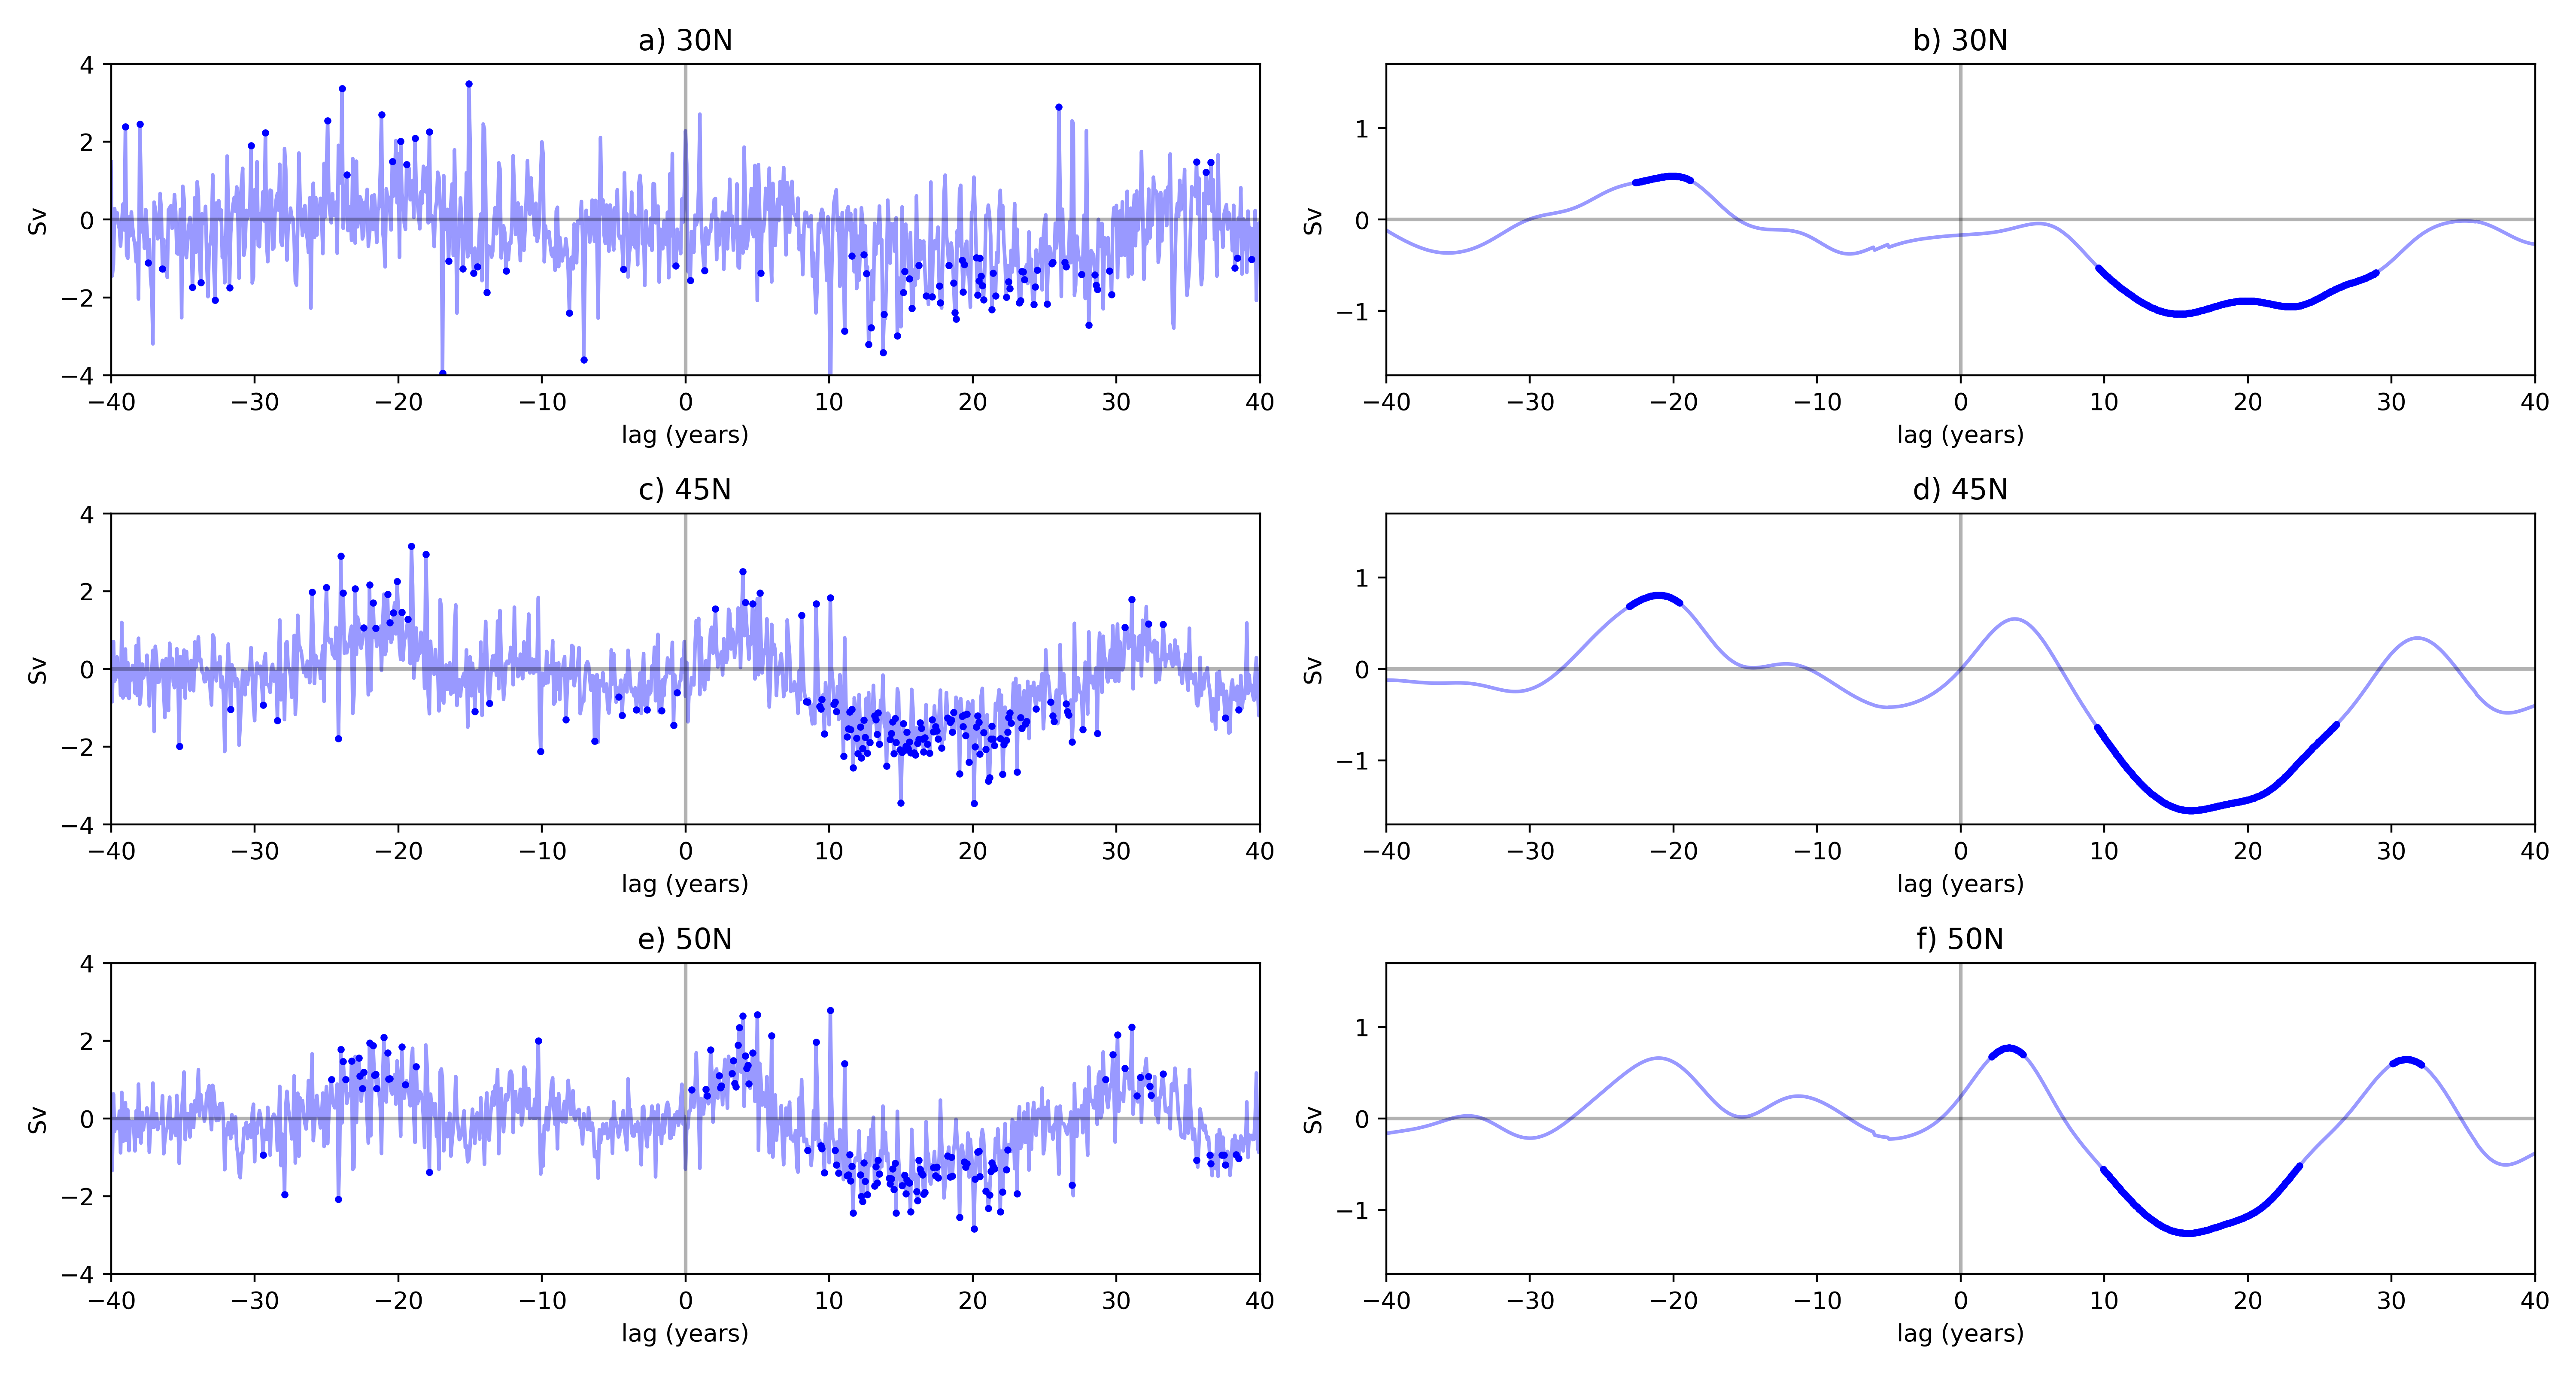
\includegraphics[width = \linewidth]{Figures/Figures-surface/AMOC_responses_low_and_highf_combined.png} 
\caption{Lagged response of AMOC index to persistent NAM$_{10}$ intervals. Blue series shows AMOC composite difference values between positive and negative NAM$_{10}$ intervals defined in section \ref{sec:model_diagnostics_surface}. The $x$ axis denotes the lead (negative values) or lag (positive values) relative to the interval's central year. Black dots denote composite differences significant at the 95\% level under a 2-tailed student's t-test. Panels a, c and e shows monthly AMOC composites which b,d and f show smoothed AMOC composites using a Gaussian filter ($\sigma$ = 2 years).}
\label{AMOC_comp_NAM}
\end{figure}
\end{center}

We now examine this vortex-AMOC teleconnection in closer detail to understand possible physical pathways responsible for an AMOC response to persistent NAM$_{10}$ intervals. figure \ref{NAO_AMOC_T_response}a shows the corresponding lead-lag composite difference analysis for the NAO filtered with the same Gaussian smoother (in green) with the smoothed 50N AMOC response (from fig \ref{AMOC_comp_NAM}f) superimposed for comparison (in blue). There is a zero-lag response in the NH winter NAO, consistent with figure \ref{fig:surface_comp_all} that indicated an in-season NAO response to an anomalous vortex event and the sign of the response is also consistent, with a positive NAO response to persistent positive NAM$_{10}$ anomalies and a negative NAO response to a persistent negative NAM$_{10}$.  There is also a significant negative anomaly in the NAO which emerges at a lag of approximately 10 years and persists up to lags of 18 years. The oscillatory response is also evident, with a positive NAO response at lags of around 28 years but with smaller amplitude than the zero-lag response. 

Also evident from figure \ref{NAO_AMOC_T_response}a is that the oscillatory responses of the NAO and AMOC are similar, with the NAO leading the AMOC response by 2-3 years. Both responses vary with periods of 28-30 years but, interestingly, the negative responses in both signals are  larger and longer-lasting at 10-20 year lags than those at zero and 28-30 year lags. This difference in the magnitude and persistence suggests that the NAO and AMOC response patterns cannot be explained as a straightforward oscillatory response to the NAM$_{10}$ forcing at zero-lag. If this were the case then the response amplitude would be expected to decay with time and the negative response at 10-20 year lag would be smaller than the initial positive response. Instead, a form of feedback mechanism is required to explain the amplified 10-20 year lagged responses or a resonant mechanism as proposed in \cite{reichlerStratospheric2012}. If such a feedback mechanism were present then one might also expect to see some oscillatory behaviour in the smoothed NAM$_{10}$ time-series, in response to the feedback from the surface. To investigate this, figure \ref{NAO_AMOC_T_response}b shows the corresponding lead-lag difference analysis for the NAM$_{10}$ index (i.e. the smoothed NAM$_{10}$ composited around its own extreme values). This supports the presence of a feedback mechanism since it also exhibits oscillatory behaviour with the same period of around 30 years. However, this oscillation is largely evident from the two positive peaks at zero-lag and 30yr-lag, with the latter being substantially damped. There is no significant response at lags of 10-20 years, where the NAO and AMOC responses were largest. This suggests that the negative NAO and AMOC responses at these lags are unlikely to be due to resonance with the NAM$_{10}$ signal. 

Alternatively, a possible physical pathway could involve a two-way amplifying feedback mechanism primarily involving  the NAO and AMOC responses. In this case, the zero-lag NAO response associated with the persistent NAM$_{10}$ intervals would drive a persistent positive ocean-atmosphere heat flux anomaly over the Labrador sea in accordance with the response patterns to individual events seen in figure \ref{fig:surface_comp_all}. This would in turn lead to persistent negative anomalies in the near-surface ocean temperatures as heat is  removed from the ocean via wind stress curl and evaporation. To explore this, figure \ref{AMOC_comp_NAM}c shows the lead-lag difference analysis for the ocean temperatures from the surface to depths of 2000m in a region encompassing the Labrador sea and part of the Central Northern Atlantic (45$^{\circ}$\,–65$^{\circ}$\,N, 15$^{\circ}$\,–60$^{\circ}$\,W). We choose to inspect temperature anomalies in this region as it covers the area over which the majority of Ocean-Atmosphere heat flux responses to individual vortex events appear (figure \ref{fig:surface_comp_all}, middle row). As a result, it is likely to highlight the forcing exerted on the deep ocean via alterations in heat exchange between the atmosphere and the ocean cause by the stratosphere. An identical region is also analysed in \cite{reichlerStratospheric2012}. A near-surface negative response is indeed evident at 0-1yr lags. Subsequently, the AMOC transport would increase due to alterations in density gradients, mixed layer depth and subsequent deep convection in the Labrador sea, an effect discussed in \cite{delworthInterdecadal1993} and \cite{medhaugMechanisms2012}. This accounts for the positive response in the AMOC at 2-3 year lags following NAM$_{10}$ intervals. This increase in AMOC strength would subsequently increases the Labrador Sea temperatures via poleward transport of heat. This is confirmed by the positive, deep (down to 2000m) ocean temperature anomaly at a lag of 10-20 years in figure \ref{NAO_AMOC_T_response}c. In turn, this reversal of the Labrador Sea temperatures can feedback onto the NAO (see e.g. \cite{frankignoulInfluence2013} by inducing a negative NAO phase at 10 years lags as the increased Labrador Sea heat content alters ocean-atmosphere heat fluxes in the same region.  Finally, this switch in the NAO phase would lead to a subsequent negative AMOC anomaly via the same heat flux mechanism in reverse. This sequence of feedbacks would thus act to enhance the persistence and magnitude of the secondary extreme in the NAO and AMOC. \cite{reichlerStratospheric2012} also briefly suggest a similar mechanism to account for the AMOC response in their simulations, but involving a negative feedback of the AMOC onto itself as well as a role for the NAO. 


\begin{figure}[h!]
\begin{center}
\noindent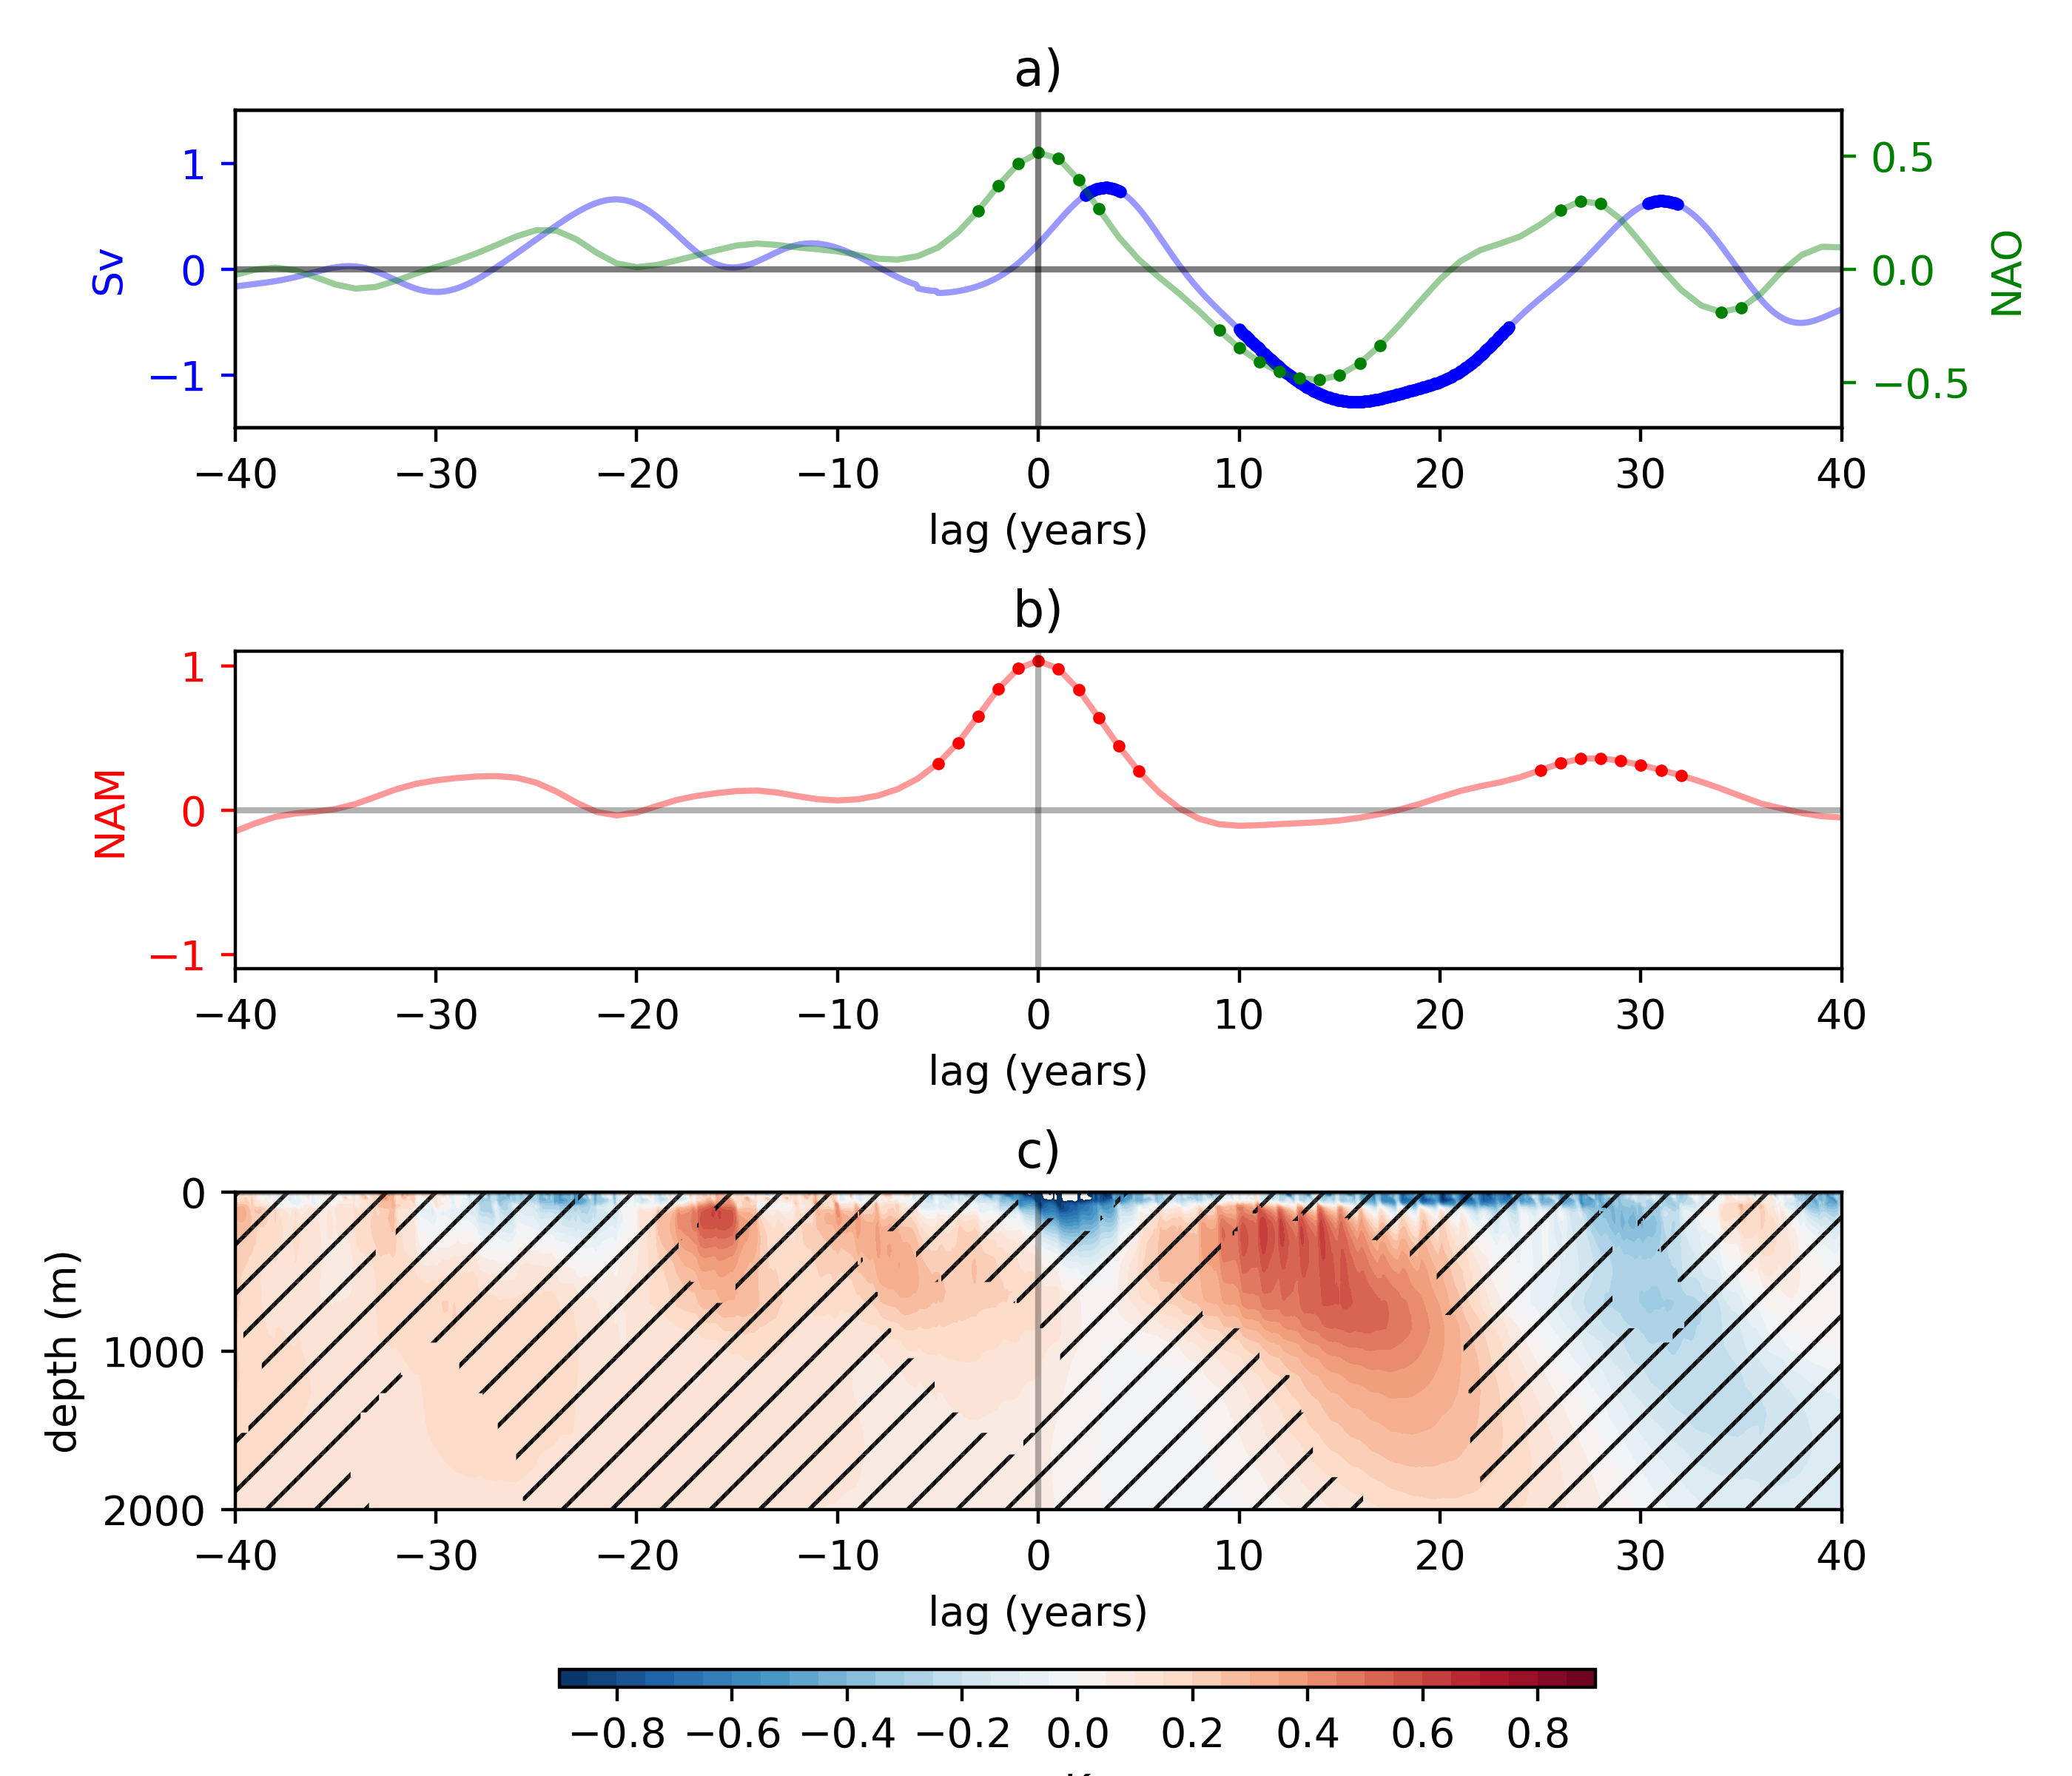
\includegraphics[width = \linewidth]{Figures/Figures-surface/Ocean_T_AMOC_NAO_responses.png} 
\caption{\textbf{a}: Like figure \ref{AMOC_comp_NAM}f for the AMOC at 50N (blue) and the Dec-Mar mean NAO index both smoothed with a Gaussian filter ($\sigma$ = 2 years). \textbf{b}: like \textbf{a} for the smoothed NAM$_{10}$ index around extreme NAM$_{10}$ intervals. \textbf{c}: lagged responses of ocean temperature anomaly depth profiles to persistent NAM$_{10}$ intervals. Composite differences between strong and weak intervals are shown for area weighted averages of an Atlantic box defined by 45$^{\circ}$–65$^{\circ}$N, 15$^{\circ}$–60$^{\circ}$W. Hatching indicates composite differences that are not significant at the 95\% level under a 2-tailed student's t-test.}
\label{NAO_AMOC_T_response}
\end{center}
\end{figure}

So far, we have considered composite difference responses to persistent strong and weak vortex intervals. However, we know that the vortex evolution during strong and weak vortex years is very different and this is likely to lead to differing interactions with surface and ocean variability.  The surface responses to the two extremes are therefore unlikely to be equal and opposite. For example, weak vortex winters are mostly associated with SSWs whose impact at the surface is observed on average 0-60 days after their central date \citep{baldwinStratospheric2001a}. Furthermore,  the vortex often exhibits a pre-conditioned state (see e.g. \cite{charltonNew2007a} and \cite{bancalaPreconditioning2012} outlined in section \ref{sec:SSW}) in which it becomes anomalously strong in the weeks running up to an SSW. So the timing of SSW events within a given season will dictate both the overall strength of the NAM$_{10}$ measured over the winter season (which we use to construct the persistent NAM$_{10}$ index) and the overall strength of the subsequent surface response. In contrast, winters that exhibit an anomalously strong vortex will, on average, exhibit such behaviour throughout the whole season so the impact on the surface will be present for a larger fraction of the winter season.

To assess the separate influences from each type of vortex extreme, figure \ref{NAO_AMOC_response_individual_types} shows the lead-lag composite analysis of the NAO, AMOC and NAM$_{10}$ signals for the persistent positive (strong vortex) and persistent negative (weak vortex) NAM$_{10}$ intervals separately. The AMOC patterns associated with each NAM$_{10}$ type manifest slightly differently. The persistently strong vortex composite shows clear oscillatory behaviour with a period of approximately 28 years. These patterns resemble many of the features observed in the AMOC composite differences associated with persistent NAM$_{10}$ intervals (figure \ref{NAO_AMOC_T_response}a). Specifically, positive AMOC at lags of 2-3 years, negative AMOC at 15-20 years and a second positive anomaly at approximately 30 years. On the other hand, the persistently weak vortex composites exhibit a more complicated response, with double peaked minima at lags of -20 and -11 years and double-peaked maxima at 14 and 25 years. The weak vortex composites also exhibit no significant AMOC response at 2-3 year lags unlike the strong vortex composites. The NAO responses exhibit greater symmetry than those for the AMOC. Both exhibit NAO anomalies at zero-lag followed by an extreme of the opposite sign at approximately 16yr and 14yr lags for strong and weak intervals respectively. As with the AMOC composites, the NAO responses to persistently strong vortex intervals exhibits a pronounced oscillatory behaviour of periods around 28 years. Finally, the corresponding NAM$_{10}$ analysis also shows oscillatory behaviour with periods of around 28 years. (We note that the NAM$_{10}$ results  show statistical significance  at both lead and lag times. However, the lead/lag interpretation is less meaningful in this case since the NAM$_{10}$ is used both as the signal and in the selection of the composites. The significance at both lead and lag times simply confirms that there is oscillatory behaviour). 

The asymmetry between the AMOC and NAO responses to persistently strong and persistently weak vortex intervals and the complexity of the separate responses show that the interactions between the NAM$_{10}$ and these surface modes are complex, with some suggestion of oscillatory behaviour on different timescales. In the following sections we address these complexities in more detail by analysing the frequency spectra of the time-series and show that some of these complexities can be explained in terms of the non-stationarity of the signals.

\begin{figure}[h!]
\begin{center}
\noindent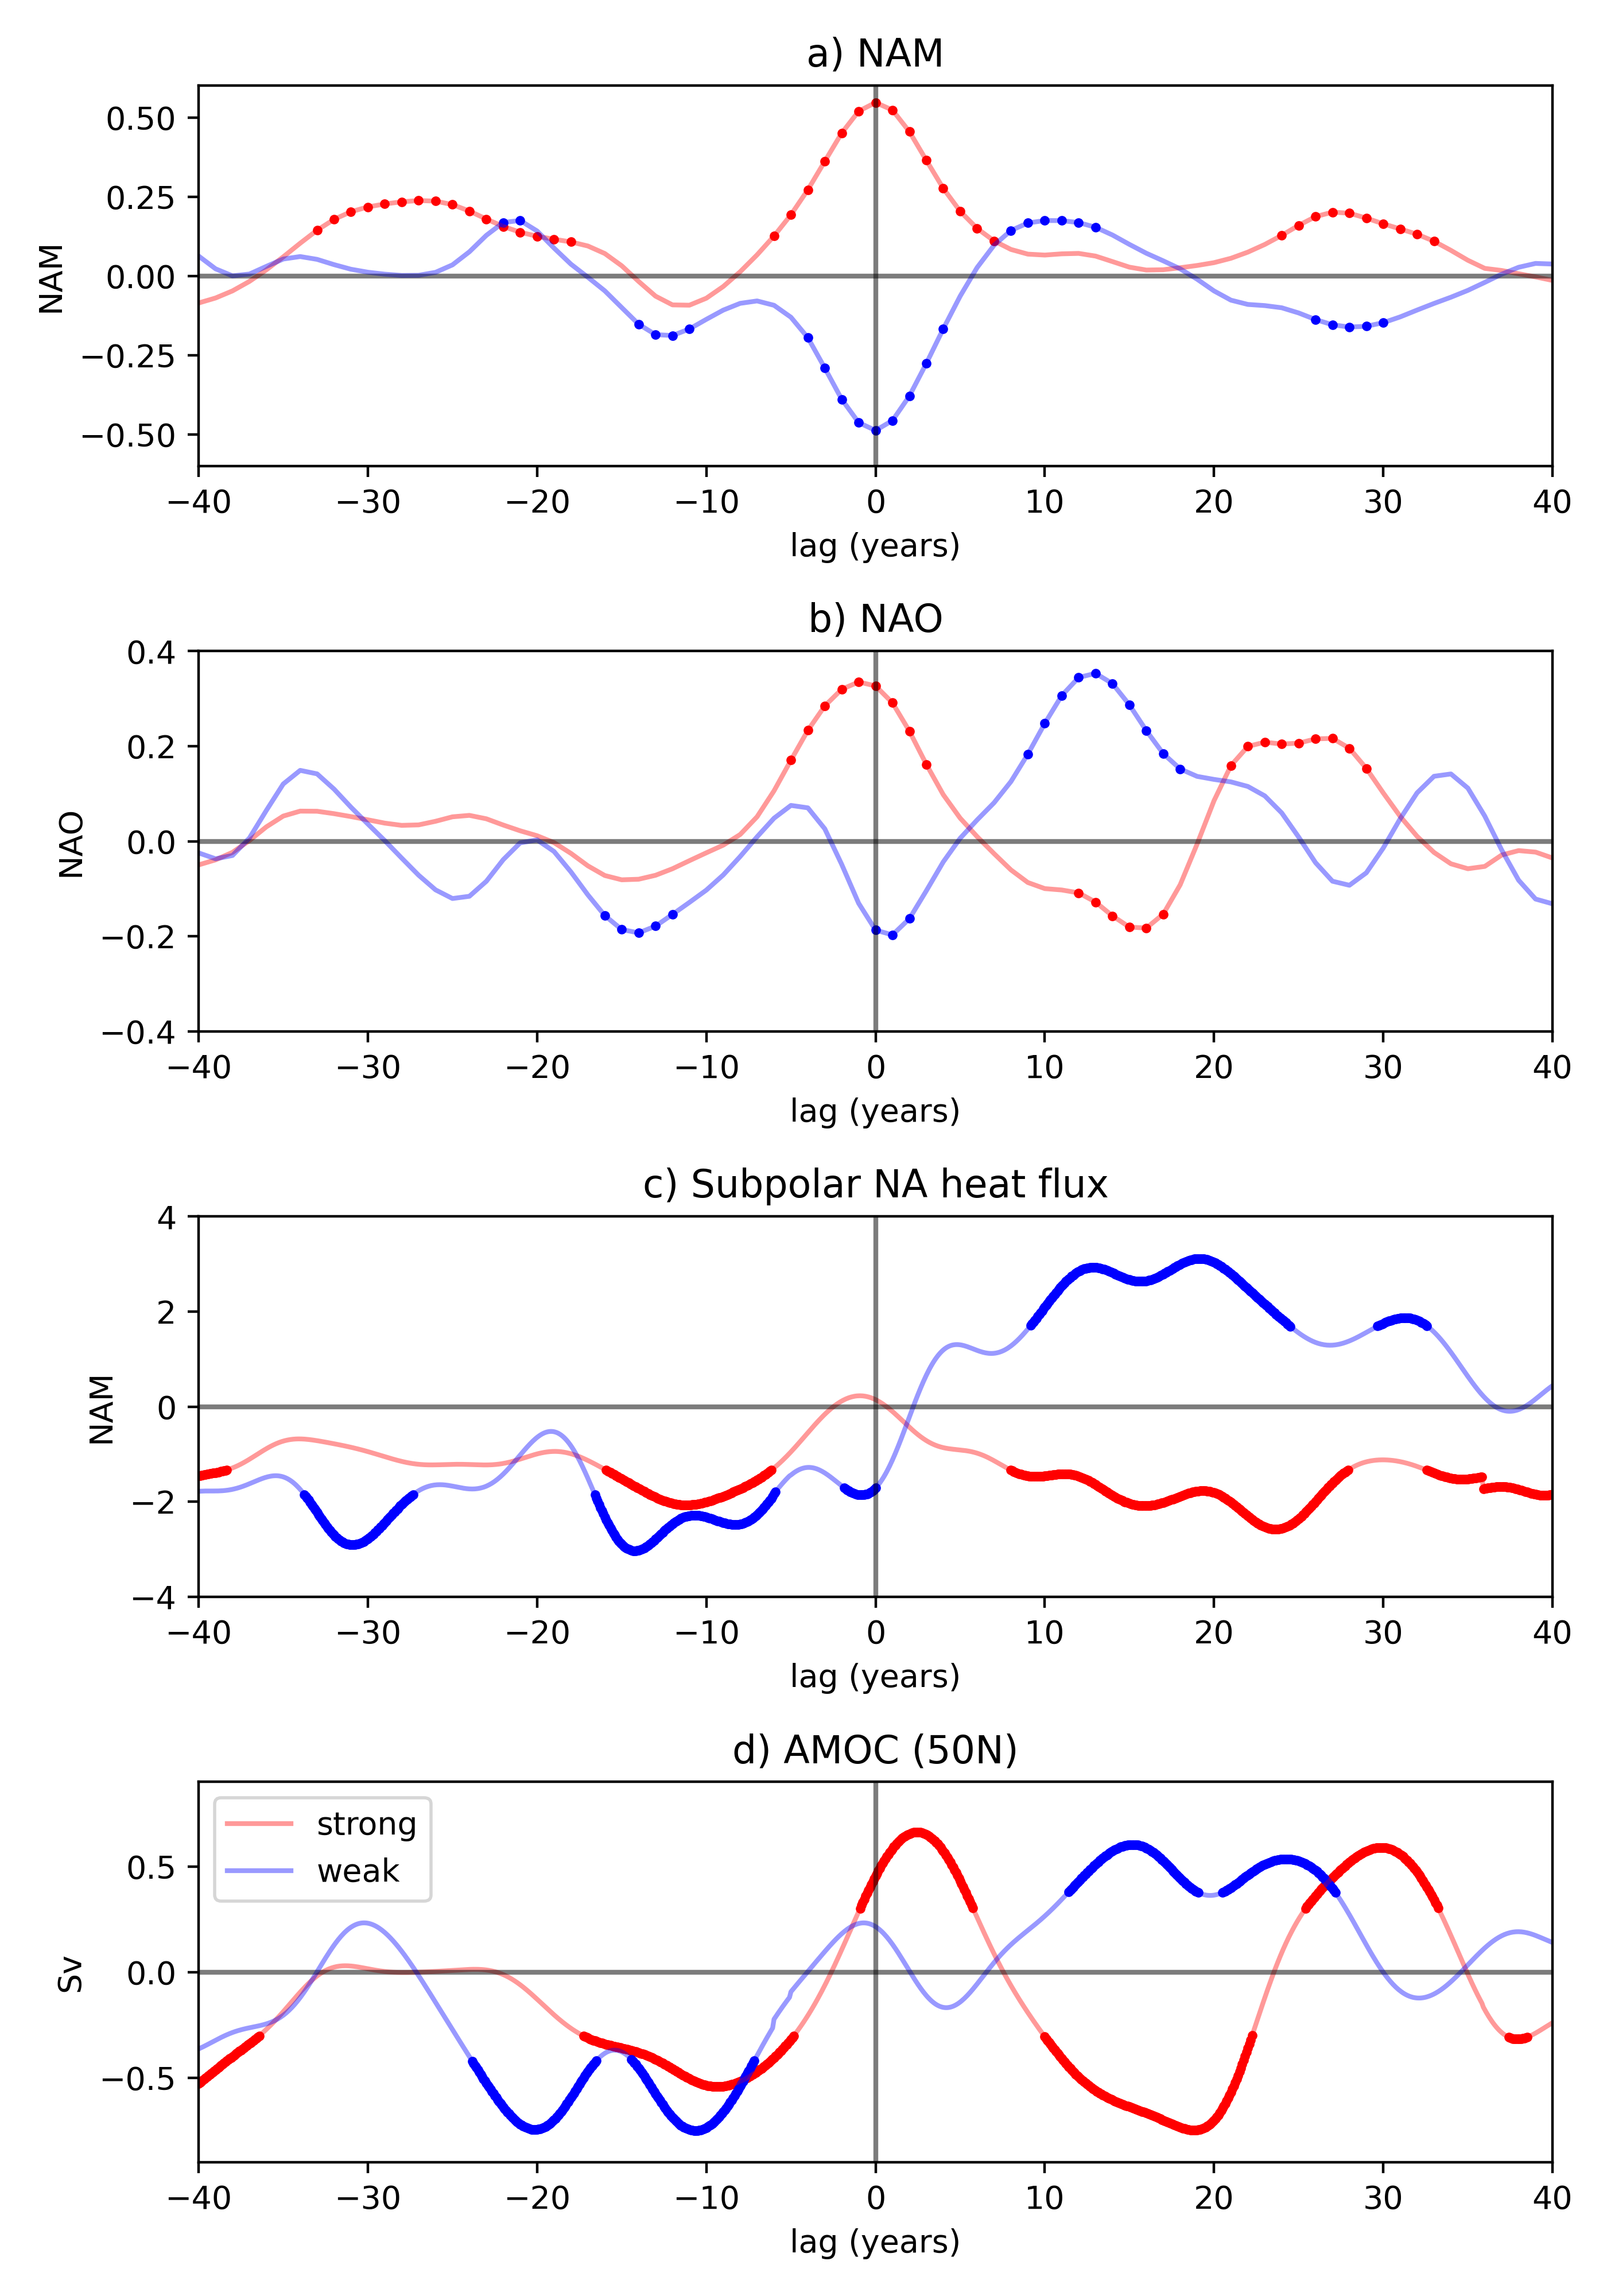
\includegraphics[width =\linewidth]{Figures/Figures-surface/AMOC_NAO_NAM_responses_each_event_type.png} 
\caption{\textbf{a}: Composites of Gaussian smoothed AMOC anomalies at 50N (a), NAO (b) and NAM$_{10}$ (c) associated with persistent vortex intervals of different types. On each sub-figure red (blue) series represent composites about strong (weak) persistent NAM$_{10}$ intervals. Solid dots denote composite anomalies significant to the 95\% level under a 2-tailed student's t-test.}
\label{NAO_AMOC_response_individual_types}
\end{center}
\end{figure}

\section{Non-Stationary Variability}
The analysis of chapter 3 showed that variability of the stratospheric polar vortex occurs on a range of timescales and is highly non-stationary (figure \ref{fig:SSW_series_5yr_wavelet}). Although the composite analysis presented above shows oscillatory behaviour with periods of approximately 30-yr the results are likely complicated by the presence of  non-stationary variability at other periodicities. We therefore analyse the frequency characteristics of the filtered NAM$_{10}$ index. Figure \ref{NAM_wavelet} shows the wavelet power spectrum of this index. It reveals variability on a range of timescales. As expected from the composite analyses, the spectrum exhibits intermittent power throughout the whole simulation at periods between 15 and 40 years. There is also significant power corresponding to a period of approximately 90-100 years that persists for $\sim$300 years of the simulation (year numbers 520-820; approximately 3 cycles) as well as power at the 50 year period timescale that persists for 120 years (year numbers 500-620; approximately 2 cycles). These features are similar to those exhibited by the SSW$_5yr$ timeseries analysis of chapter 3 but not identical, since their time-series was a measure of SSW frequency whereas figure \ref{NAM_wavelet} uses the time-series of smoothed NAM${_10}$ anomaly and therefore provides a measure of persistently strong as well as persistently weak vortex intervals.

The three periodicities  around 30-, 50- and 90-years are also highlighted by the so-called 'global wavelet spectrum' (see figure \ref{NAM_wavelet}), which is an average measure of power over the whole simulation, and shows three peaks in power corresponding to periods of approximately 25, 50 and 90 which are all deemed significant when compared to the spectrum of a theoretical red noise process (see section \ref{sec:Wavelet_Analysis}). We note that much of the $\sim$30-yr periodicity seen in the composite analysis is likely associated with significant wavelet power in the interval between years 300 and 410 and this interval displays the largest number of positive extremes in the smoothed NAM$_{10}$ time-series (compare the 30-yr wavelet power in figure \ref{NAM_wavelet} with the red dots in figure \ref{NAM_and_filtered}). The large number of elevated filtered NAM$_{10}$ extremes selected in this interval is also likely affected by the presence of extremely long timescales variability: qualitative inspection of figure \ref{NAM_and_filtered} shows that the underlying NAM$_{10}$ amplitude increases from around year 200, reaches a peak at $\sim$year 380 and thereafter declines. This means that years within this interval are more likely to reach the top 5 percentile and qualify as an anomalously strong vortex. The origin of this multi-centennial variability is unclear and robust analysis of such a low frequency signal is difficult as the wavelet power is located mostly outside the so called "cone of influence" (blue shading and black hatching on figure \ref{NAM_wavelet}) that marks the boundary at which edge effects become significant. 

\begin{figure}[h!]
\begin{center}
\noindent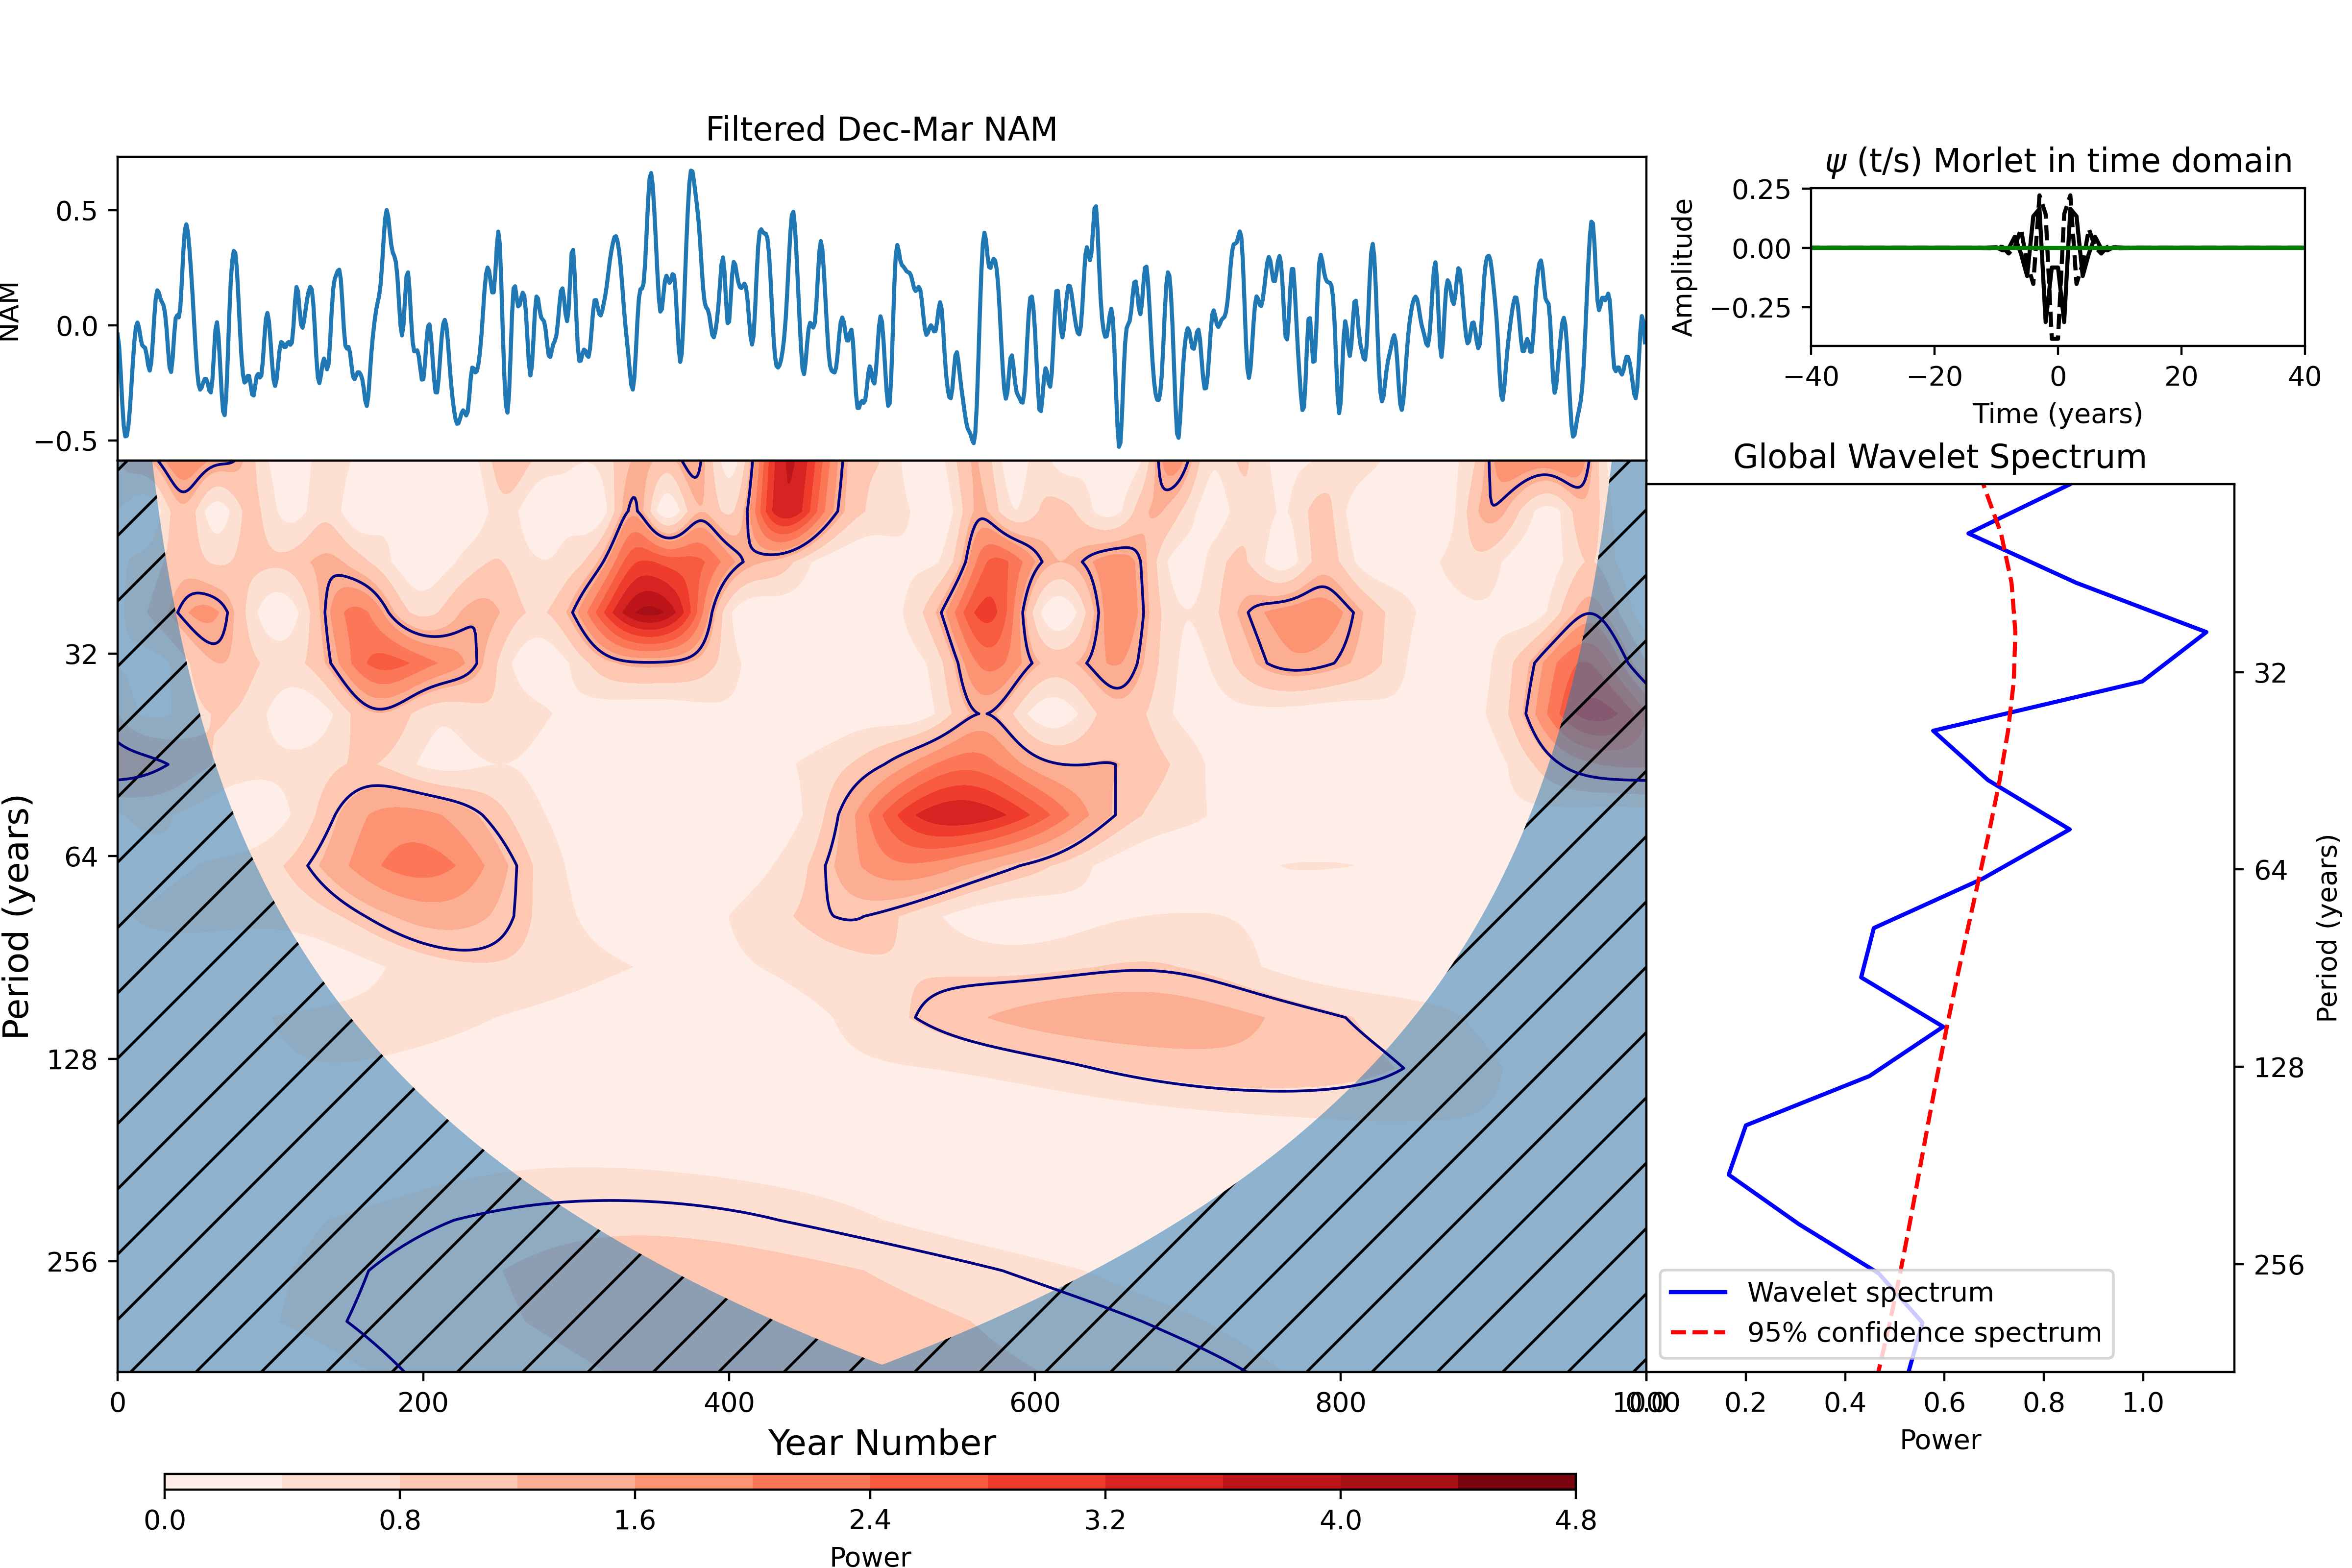
\includegraphics[width = 0.8\linewidth]{Figures/Figures-surface/NAM_wavelet_UKESM.png}
\caption{\textbf{Top left}: Dec-Mar NAM$_{10}$ values smoothed with a with a Gaussian filter ($\sigma$ = 2 years). \textbf{Bottom left}: Wavelet power spectrum of time series in top left. Hatching represents area outside the cone of influence in which edge effects are significant and power should not be considered. Navy contours represent the 95\% confidence level assuming mean background AR1 red noise. \textbf{Top Right}: Morlet wavelet used for the wavelet transform in the time domain. \textbf{Bottom right:} Global power spectrum, the wavelet power averaged over the whole simulation (blue line), and global 95\% confidence spectrum (red dashed line).}
\label{NAM_wavelet}
\end{center}
\end{figure}

A natural question following from the assessment of stratospheric variability in figure \ref{NAM_wavelet} is whether the AMOC variability reflects this? Figure \ref{NAM_AMOC_Cross} shows the corresponding wavelet spectra of the AMOC at 50N and also the cross wavelet spectra between the filtered NAM$_{10}$ and the AMOC which gives a time varying measure of co-variability between signals in the indices at different periods. The wavelet spectrum for the AMOC at 50N exhibits a peak in spectral power corresponding to approximately 130 years that persists for nearly 400 years of the simulation (and also at longer periods up to 250 years but boundary effects are an issue at these multi-centennial timescales, as discussed above). There are also portions of significant power at approximately 30 year and 50 year periods, both of which persist for approximately 2 cycles ($\sim$60 years and $\sim$100 years respectively). These three features are also apparent in the global power spectrum. The 30-yr periodicity is not sustained throughout the whole simulation, so the global power spectrum does not achieve statistical significance at this periodicity, but note that the main 30-yr power comes from the 300-400 year interval, coinciding with the interval of most activity in both the NAM$_{10}$ analysis (figure \ref{NAM_wavelet}) and the selected high NAM$_{10}$ percentiles (figure \ref{NAM_and_filtered}). 
 
The cross power spectrum between the filtered NAM$_{10}$ and the AMOC shows 3 distinct features corresponding broadly to the three timescales prominent on the individual spectra of both indices. Significant cross power is evident at 90-100 year periods for approximately 350 years (between 450 and 800 years; 3-4 cycles). The phase relationship between the signals (indicated by arrows on figure \ref{NAO_NAM_Cross}) within this portion of the cross spectrum  show a mixture of left-pointing arrows in the earlier portion, which indicate an anti-correlated relationship  ($\pi$ out of phase) and downward pointing arrows in the later portion that indicate a $\frac{\pi}{2}$ phase relationship. This latter can be interpreted in a number ways, with maxima in the AMOC leading to maxima in the NAM$_{10}$, minima in the NAM$_{10}$ leading to maxima in the AMOC or maxima in the NAM$_{10}$ index coinciding with maxima in the rate of change of the AMOC (see section \ref{sec:Wavelet_Analysis} for details on cross spectra arrows). There is also significant cross spectral power centred around 30 years (between 300-400 years; 3 cycles) and 50 years (between 500-600 years; 2 cycles). In contrast to the 90-yr periodicity, the phase arrows point to the right and slightly upwards, indicating that maxima in the NAM$_{10}$ index lead to maxima in the AMOC by a small fraction of the cycle. This phase relationship on the 30-yr and 50-yr timescales is consistent with the composite analysis presented in figures \ref{AMOC_comp_NAM} and \ref{NAO_AMOC_response_individual_types} that indicated that a positive (negative) NAM$_{10}$ leads to a positive (negative) AMOC response approximately 2-3 years later. The wavelet spectra for the AMOC at 30N and 45N are provided in figures \ref{NAM_AMOC_Cross_30}a and \ref{NAM_AMOC_Cross_45}a. They show broadly the same features as that of the AMOC at 50N however it is notable that the AMOC at 30N does not exhibit significant variability on the 50 and 30 year timescales. This is reflected in the cross spectrum with the smoothed NAM$_{10}$ index which shows minimal cross power on these timescales (figure \ref{NAM_AMOC_Cross_30}b). This is consistent with figure \ref{AMOC_comp_NAM}b which indicates minimal 30 year timescale modulation of the AMOC at 30N by extremes in the smoothed NAM$_{10}$.

\begin{center}
\begin{figure}[h!]
\noindent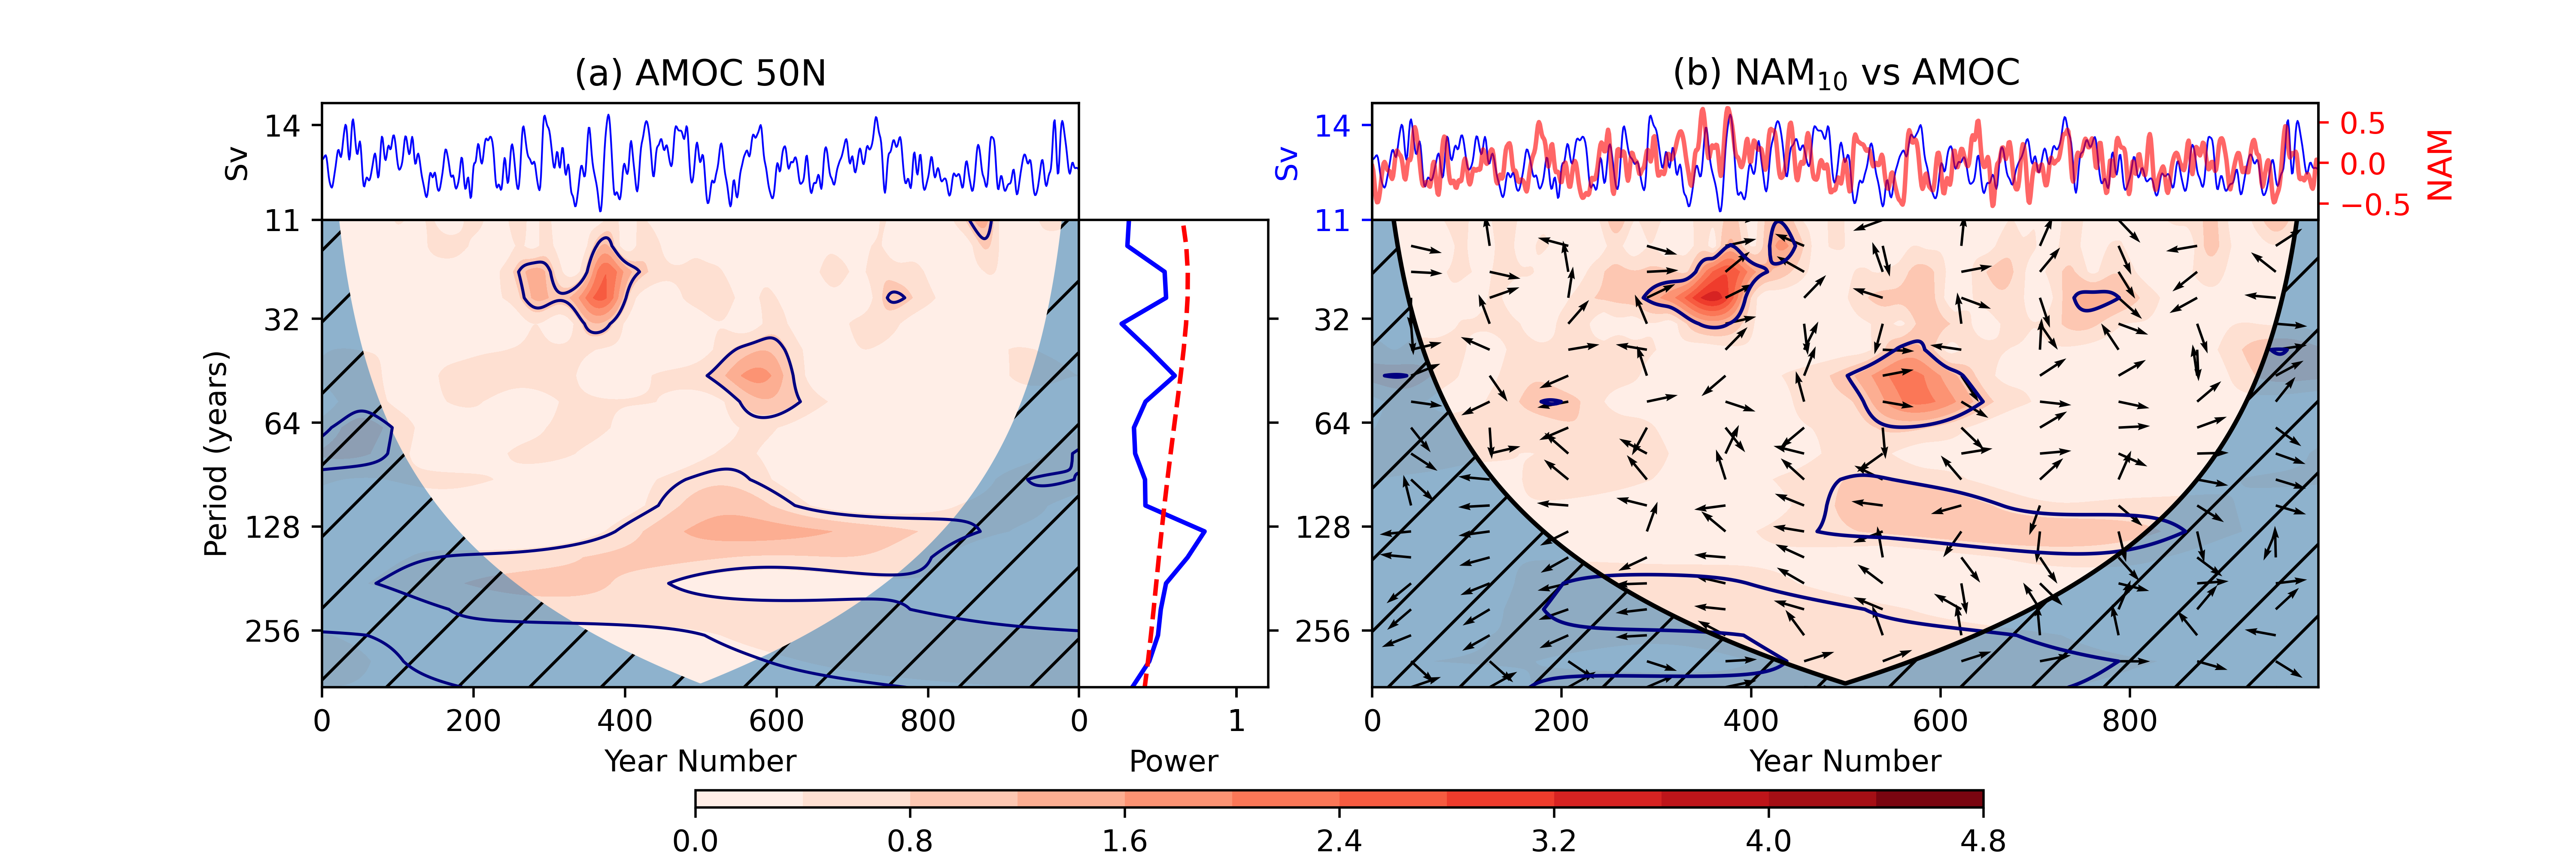
\includegraphics[width = \linewidth]{Figures/Figures-surface/AMOC_NAM_filtered_subplot.png}
\caption{\textbf{(a, top)}: AMOC time series at 50N, \textbf{a, bottom left}: Wavelet power spectrum (shaded contours represent wavelet power and yellow contours the 95\% significance level compared to an AR1 process), \textbf{a, bottom right}: global wavelet power spectrum (blue) and 95\% confidence level (dashed red). \textbf{b}: Cross spectra between Filtered Dec-Mar NAM$_{10}$ series and the AMOC index. \textbf{b, top}: NAM$_{10}$ and AMOC time series. \textbf{b, bottom}: Cross power spectrum. Shading indicates cross power, yellow contours the 95\% confidence interval and arrows the relative phase angle between signals in the time series (to the right: in phase, vertically upwards: $\frac{\pi}{2}$ out of phase with positive peaks in the NAM$_{10}$ leading those in the AMOC, to the left: $\pi$ out of phase, vertically downwards: $\frac{\pi}{2}$ out of phase with positive peaks in the AMOC leading those in the NAM).}
\label{NAM_AMOC_Cross}
\end{figure}
\end{center}

\begin{center}
\begin{figure}[h!]
\noindent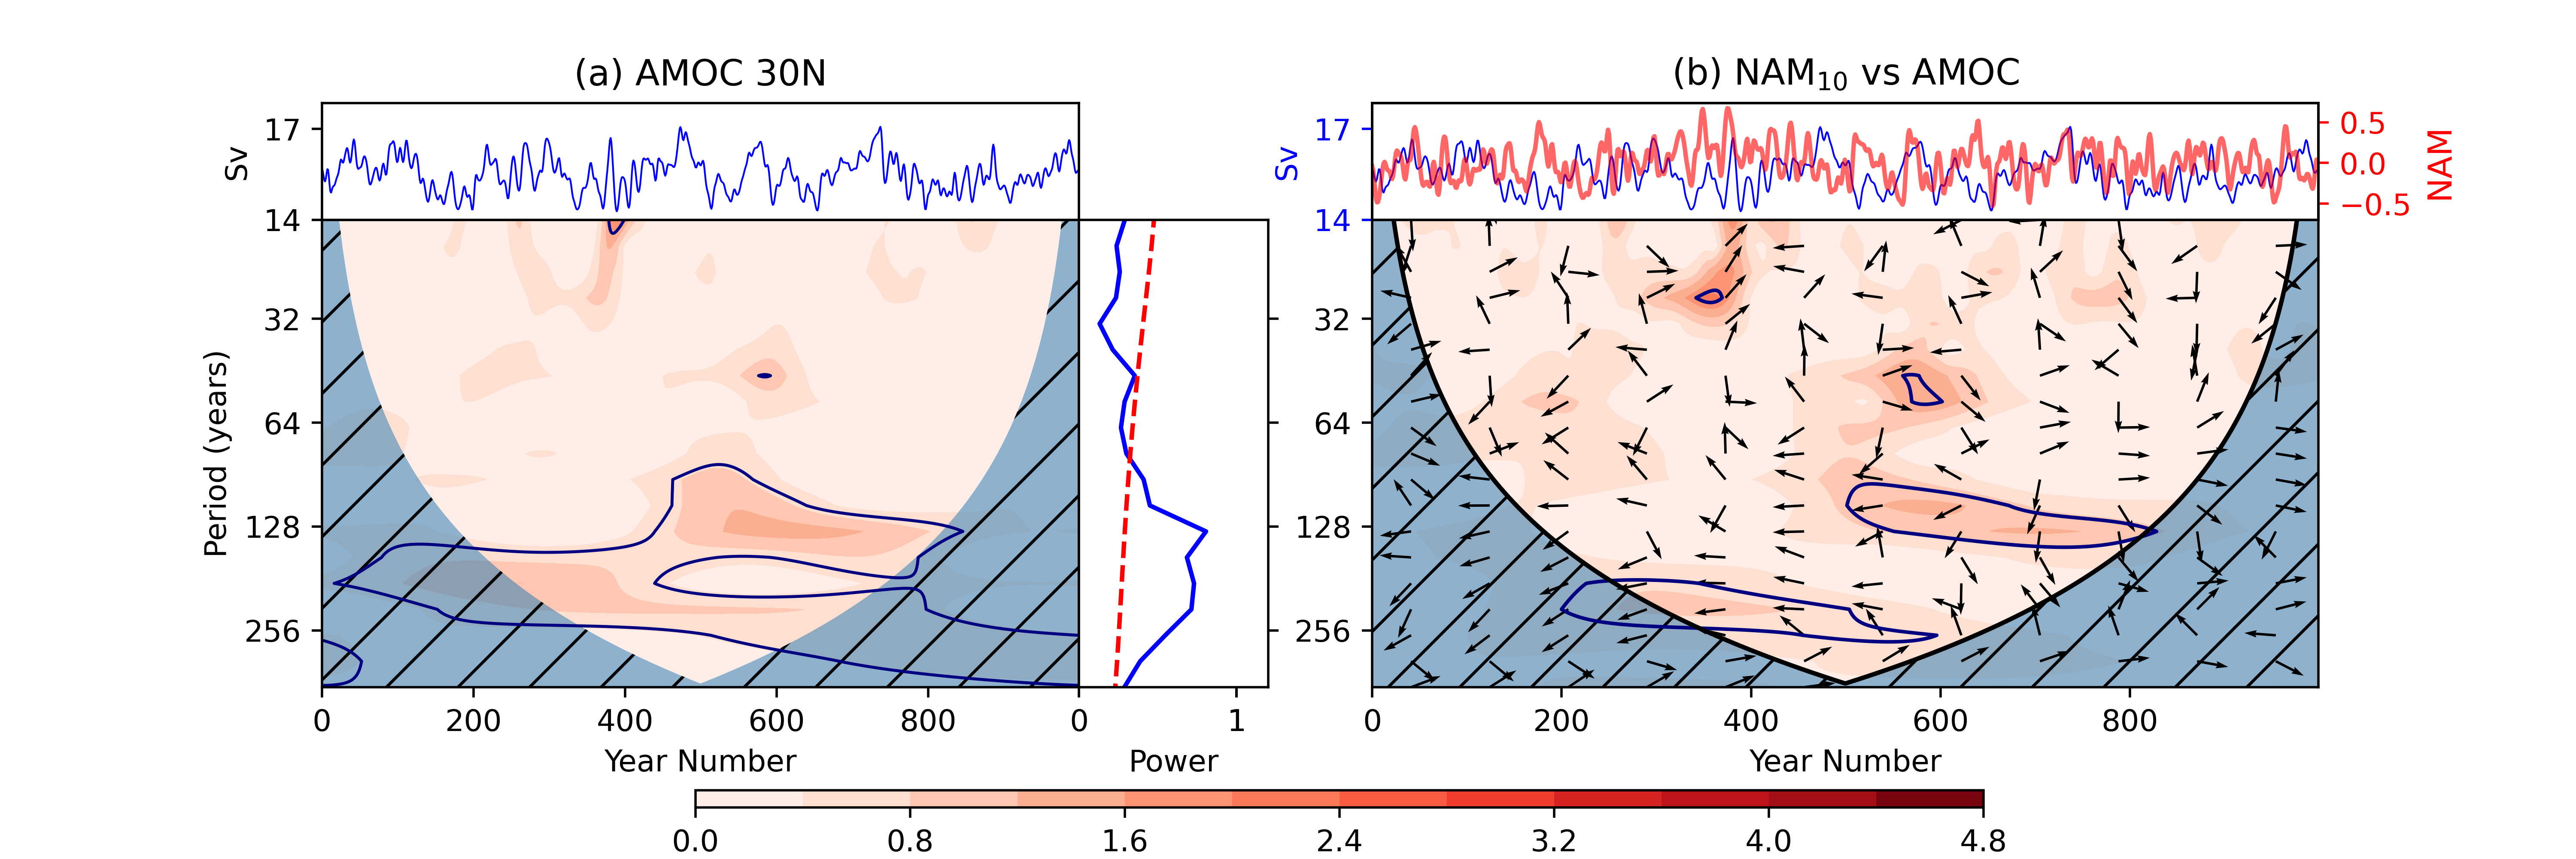
\includegraphics[width = \linewidth]{Figures/Figures-surface/AMOC_NAM_filtered_subplot_30N.png}
\caption{like figure \ref{NAM_AMOC_Cross} for the AMOC at 30N. \textbf{a} shows the wavelet power spectrum of the AMOC and \textbf{b} the cross power spectrum between the AMOC and the NAM$_{10}$ index.}
\label{NAM_AMOC_Cross_30}
\end{figure}
\end{center}

\begin{center}
\begin{figure}[h!]
\noindent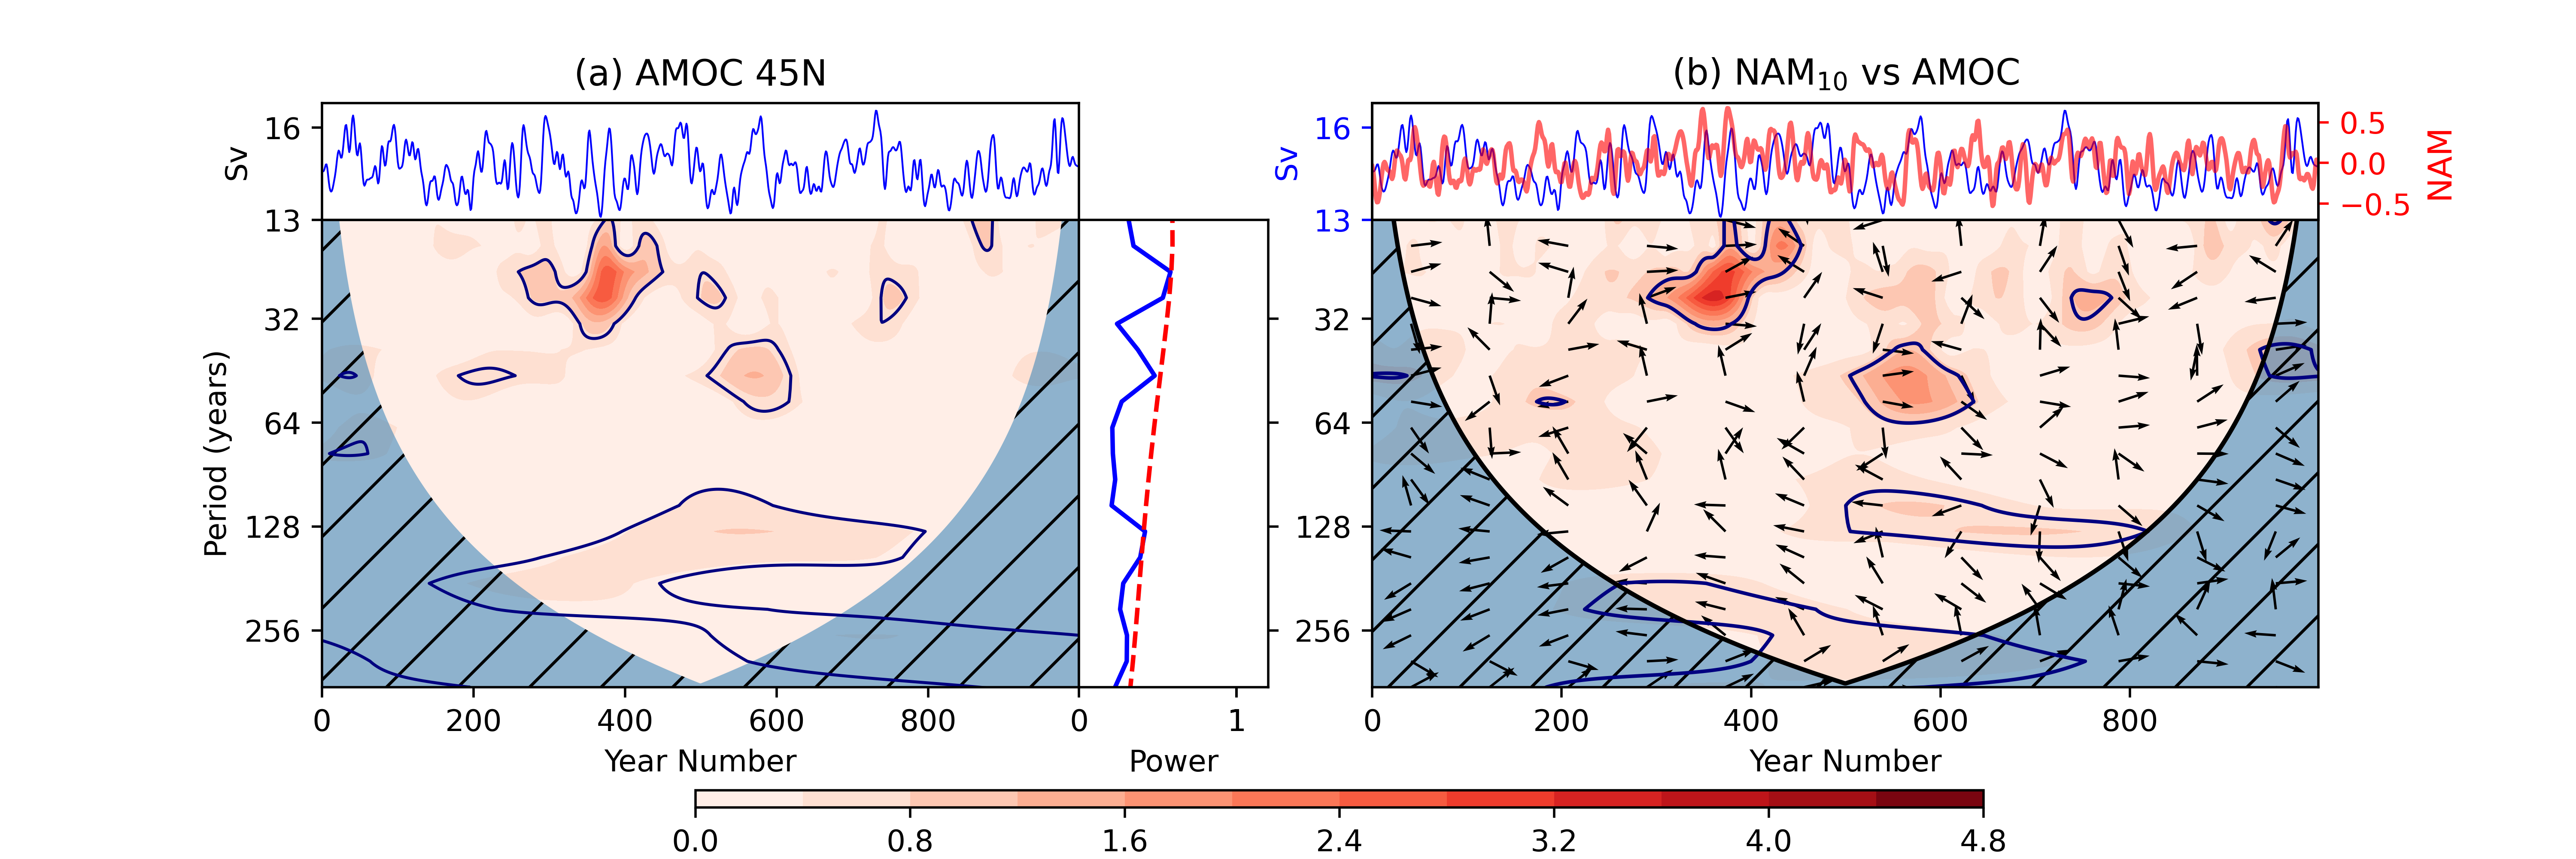
\includegraphics[width = \linewidth]{Figures/Figures-surface/AMOC_NAM_filtered_subplot_45N.png}
\caption{like figure \ref{NAM_AMOC_Cross} for the AMOC at 45N. \textbf{a} shows the wavelet power spectrum of the AMOC and \textbf{b} the cross power spectrum between the AMOC and the NAM$_{10}$ index.}
\label{NAM_AMOC_Cross_45}
\end{figure}
\end{center}
  
To understand these non-stationary signals in the context of the proposed mechanism for vortex-AMOC interactions involving the NAO, we also analyse the power spectrum for the Dec-Mar NAO as well as its cross spectra with the filtered NAM$_{10}$ index (figure \ref{NAO_NAM_Cross}). The wavelet power spectrum for the NAO (figure \ref{NAO_NAM_Cross}a) exhibits some similar features to those of the NAM$_{10}$ and the AMOC. Namely, a portion of significant power at periods of 30 years between $\sim$300-400 years as well as a feature at 50 years between $\sim$500-600 years. Furthermore, the cross power spectrum between the NAO and the NAM$_{10}$ indicate that signals in the two indices on the $\sim$30 and $\sim$50 year periods are also coincident in time for the 70-100 years they persist for. The phase relationship between these signals is small (arrows pointing to the right) indicating an in-phase relationship between the indices, which is consistent with the zero-lag relationship between the NAO and filtered NAM$_{10}$ extremes presented in composite analysis (figures \ref{NAO_AMOC_T_response} and \ref{NAO_AMOC_response_individual_types}). These coincident 30-yr and 50-yr signals between the NAM, AMOC and NAO in these intervals provide supporting evidence for an interaction between these modes of variability. However, the NAO wavelet analysis shows no significant power on the 90-100 year timescale and the prominent feature seen in both the NAM$_{10}$ and AMOC analysis is absent. This suggests that the co-variability between the NAM$_{10}$ and AMOC on these longer timescales does not involve the NAO and is likely to arise through different mechanisms. We return to examine this feature in more detail in section \ref{surface-strat_forcing}.

\begin{figure}[h!]
\begin{center}
\noindent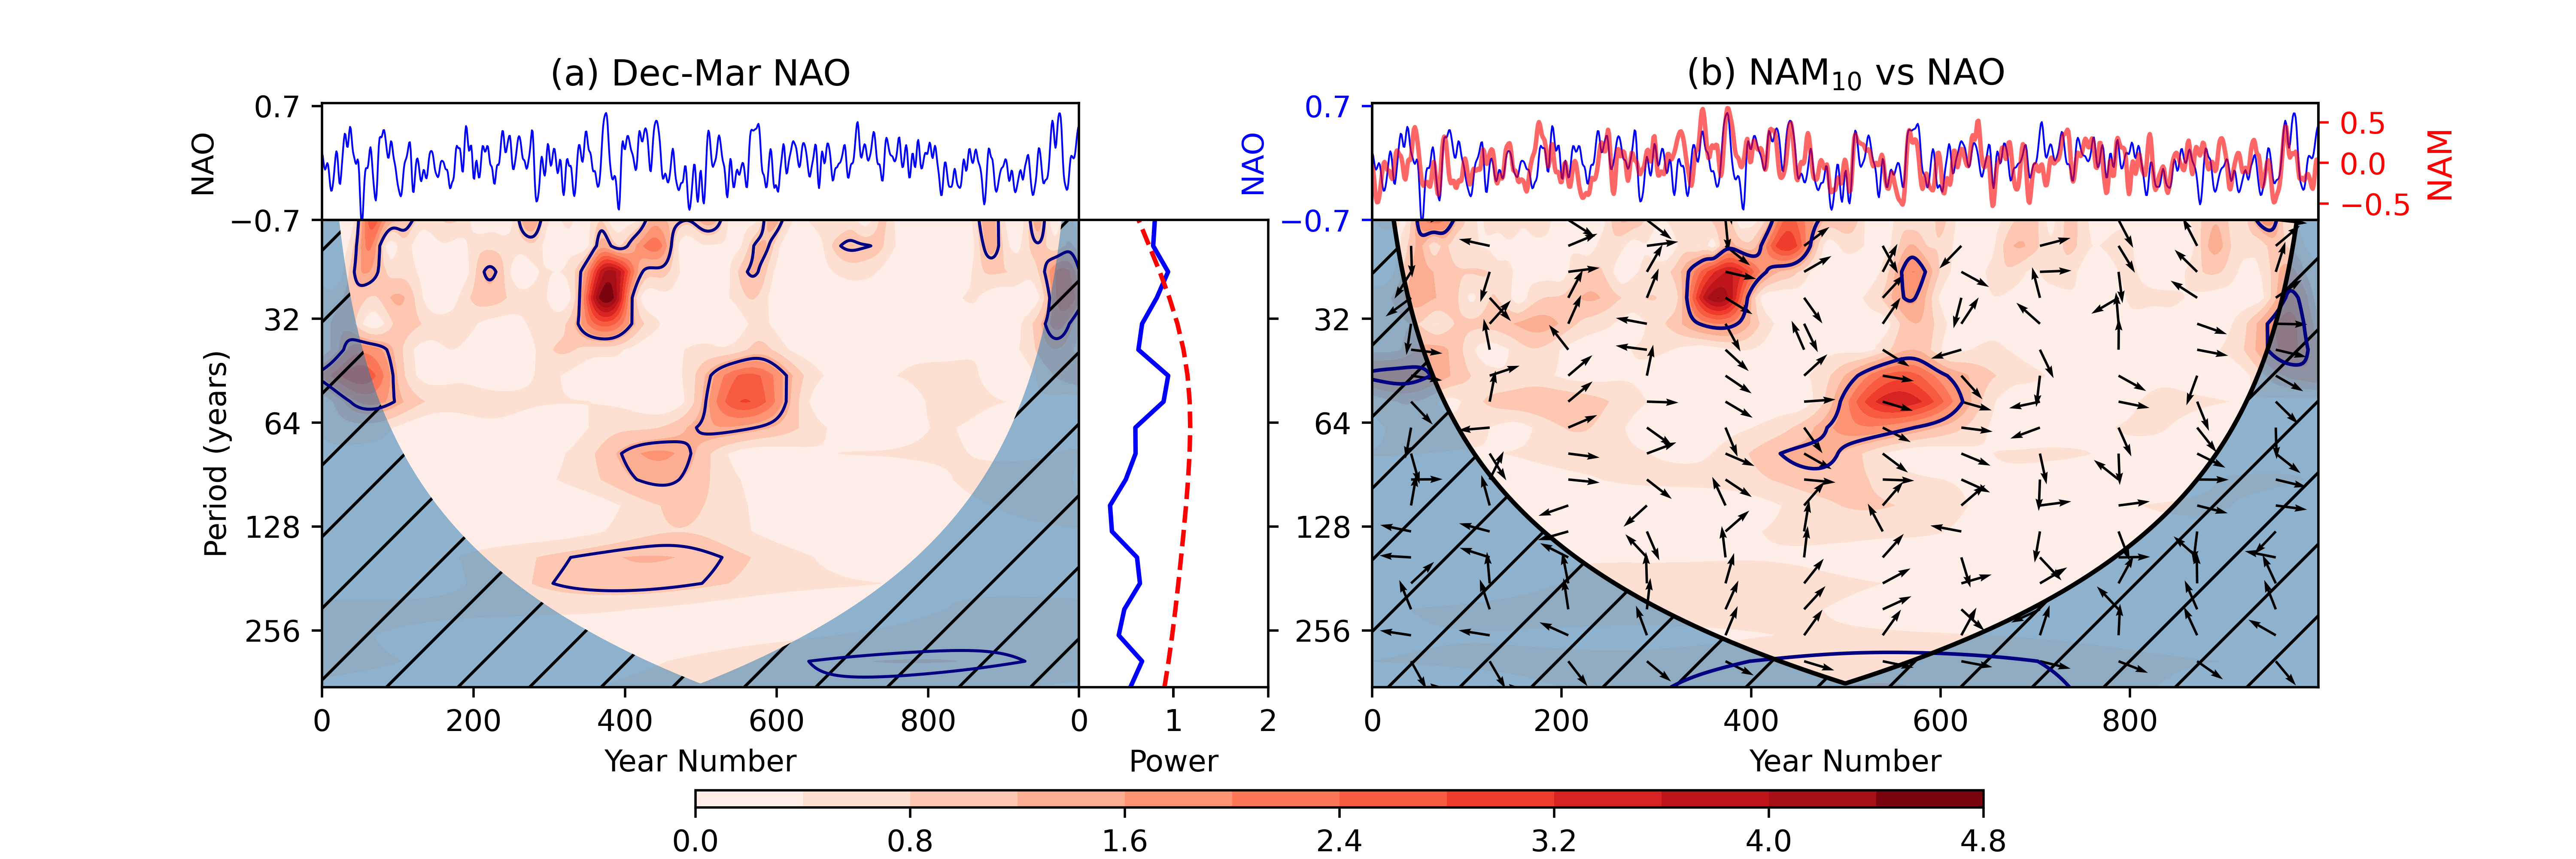
\includegraphics[width = \linewidth]{Figures/Figures-surface/NAM_NAO_filtered_subplot.png}
\caption{like figure \ref{NAM_AMOC_Cross} for the Dec-Mar NAO index. a shows the wavelet power spectrum of the NAO and b the cross power spectrum between the NAO and the NAM$_{10}$ index.}
\label{NAO_NAM_Cross}
\end{center}
\end{figure}

The wavelet analysis suggests that while 30-yr periodicity is most apparent in the composite patterns of figure \ref{NAO_AMOC_T_response} there may also be contributions involving the 50-yr and 90-yr periodicities. This complication is more clearly evident in figure \ref{NAO_AMOC_response_individual_types} where the composites associated with persistent positive and negative NAM$_{10}$ intervals were examined separately. Firstly, we note that the contribution to the composites from the interval exhibiting $\sim$30-year oscillatory behaviour ($\sim$300-400 years) comes solely from a collection of persistent strong NAM$_{10}$ intervals (see the red dots on figure \ref{NAM_and_filtered}). In contrast, a high proportion of the weak NAM$_{10}$ contributions to the composite analysis (8 out of 13) occur within the interval between $\sim$500-600 years which exhibits variability at both 50yr and 90yr periodicity. The complicated double peaked behaviour of the AMOC response following persistent weak vortex intervals can now be better understood, taking into account the influence of the $\sim$50yr and $\sim$90yr periodicities. The double minima in AMOC response at 10yr and 20yr leads and at 15yr and 25yr lags can now be explained as manifestations of the 50-yr and 90-yr AMOC responses e.g. a half-cycle between the minimum at 10yr lead and maximum at 15yr lag (thus a half-cycle of 25 years) gives a periodicity of 50yrs, while a half-cycle between the minimum at 20yr lead and 25yr lag (thus a half-cycle of 45yrs) give a periodicity of 90yrs.  Additional support for this interpretation comes from the fact that the NAO composite analysis (figure 5b) shows a response that corresponds broadly with the AMOC minimum at 10yr lead and maximum at 15yr lag, suggesting a mechanism that involves the NAO on the 50-yr timescale but there is no corresponding response in the NAO at the 90-yr periodicity, in agreement with  the wavelet spectra and cross spectra in figure \ref{NAO_NAM_Cross} which indicates that the NAO does not exhibit variability on timescales of $\sim$90 years. 

\section{Surface Forcing of the Stratosphere}\label{surface-strat_forcing}
The absence of an NAO signal that corresponds to the 90-yr periodicities seen in both the separate NAM$_{10}$ and AMOC wavelet spectra and in the  AMOC-NAM cross spectrum (figure \ref{NAM_AMOC_Cross}) indicates that the mechanism for the stratosphere - AMOC teleconnection on this longer timescale may be distinct in nature to those observed at 30 and 50 year periods. As noted earlier, the phase relationship associated with this feature is also different to the shorter timescales ($\frac{\pi}{2}$ out of phase) suggesting the possibility that the direction of causality may also be switched i.e. it may be that the AMOC leads the stratosphere response on these timescales rather than vice versa. To study this more closely we investigate possible pathways involving variability on this timescale.

In our earlier analysis of this UKESM pi-control simulation from chapter 3 we highlighted the $\sim$90-yr variability in frequency of SSWs and demonstrated that this was closely associated similar timescale variations in the amplitude of the deep QBO (and in particular, the westerly QBO phase).  Figure \ref{OLR_wavelet}a shows the wavelet spectrum of the same QBO index employed in chapter 3 smoothed with the Gaussian filter utilised throughout this work (see \ref{fig:QBO_SSW_subfig}). A portion of significant power at $\sim$90 year periods persists for approximately 200 years of the simulation between years 600-800, which coincides with the significant response in the same interval of the NAM$_{10}$ and AMOC spectra at 90yr periodicity. Cross spectra with the smoothed NAM$_{10}$ index (figure \ref{OLR_wavelet}b) also corroborates the findings from chapter 3 with coincident signals at the 90 year timescales and right-pointing arrows that indicate an in-phase relationship, so that an interval of persistently strong positive (westerly) QBO anomalies  corresponds to an interval of persistent positive (strong) polar vortex intervals (and hence a positive NAM$_{10}$ anomaly). The sign of this teleconnection is consistent with the well-known Holton-Tan teleconnection \citep{luDecadalscale2008, luMechanisms2014} but it acts on longer timescales and DM21 showed that it originates primarily from long-term variations in the strength of the westerly QBO phase. 

While the long-timescale QBO-vortex teleconnection was demonstrated in chapter 3 (and confirmed here), the cause of the long-term westerly QBO variability was not established. In a preliminary investigation, a wavelet analysis was performed on equatorial SSTs in various regions, including the equatorial East Pacific, to explore whether the $\sim$90-yr QBO variability could be explained via SST triggering of  convective activity that generates the gravity and other equatorial waves that contribute to the QBO. However, no 90-year periodicity in equatorial SSTs was found. A similar analysis of the strength of the Aleutian Low, that could perhaps explain the signals in both the QBO and the polar vortex via a modulation of the strength of large-scale planetary wave forcing, similarly found no periodicity at 90 years. Nevertheless, the extremely long period of the QBO and vortex variations suggest a driving mechanism that is linked to the oceans due to the characteristic long oceanic timescales. 

To extend this investigation, we examine variability of the East Pacific top-of-atmosphere outgoing longwave radiation (OLR) as an alternative proxy for deep convection in the region. When deep convection is enhanced, cloud top height is increased and therefore OLR is reduced. Figure \ref{OLR_wavelet}c shows the wavelet analysis of Sep-Nov  OLR in the East Pacific. It exhibits 90 year periodicity, as well as significant cross power with the smoothed QBO amplitude and the NAM$_{10}$ index (figures \ref{OLR_wavelet}d,e). The signals in the OLR and both the QBO and NAM$_{10}$ are anti-correlated (left pointing arrows indicating a $\pi$ phase difference). This is consistent with reduced OLR (increased deep convection) leading to greater QBO amplitude through increased wave forcing.  The corresponding cross spectra between the AMOC and the OLR metric (figure \ref{OLR_wavelet}f) also indicates a significant portion of cross power in the interval $\sim$600-800 years co-located with the feature seen in the NAM$_{10}$ spectrum (figure \ref{OLR_wavelet} dashed contours). The phase relationship in this case is mostly $\frac{\pi}{2}$ (the majority arrows pointing upwards) indicating that one of the quantities depends on the time rate of change of the other. This relationship is reminiscent of results from \cite{timmermannENSO2005} who show sensitivity of the equatorial Pacific region to 35 year periodic forcing of North Atlantic MOC. Their study showed a dependence of the Pacific thermocline to the rate of change of the AMOC. We therefore suggest this as a possible pathway for 90 year variability in the AMOC to influence the stratospheric NAM, through changes in deep convection in the East Pacific that influences the amplitude of the QBO. 


\begin{figure}[h!]
\begin{center}
\noindent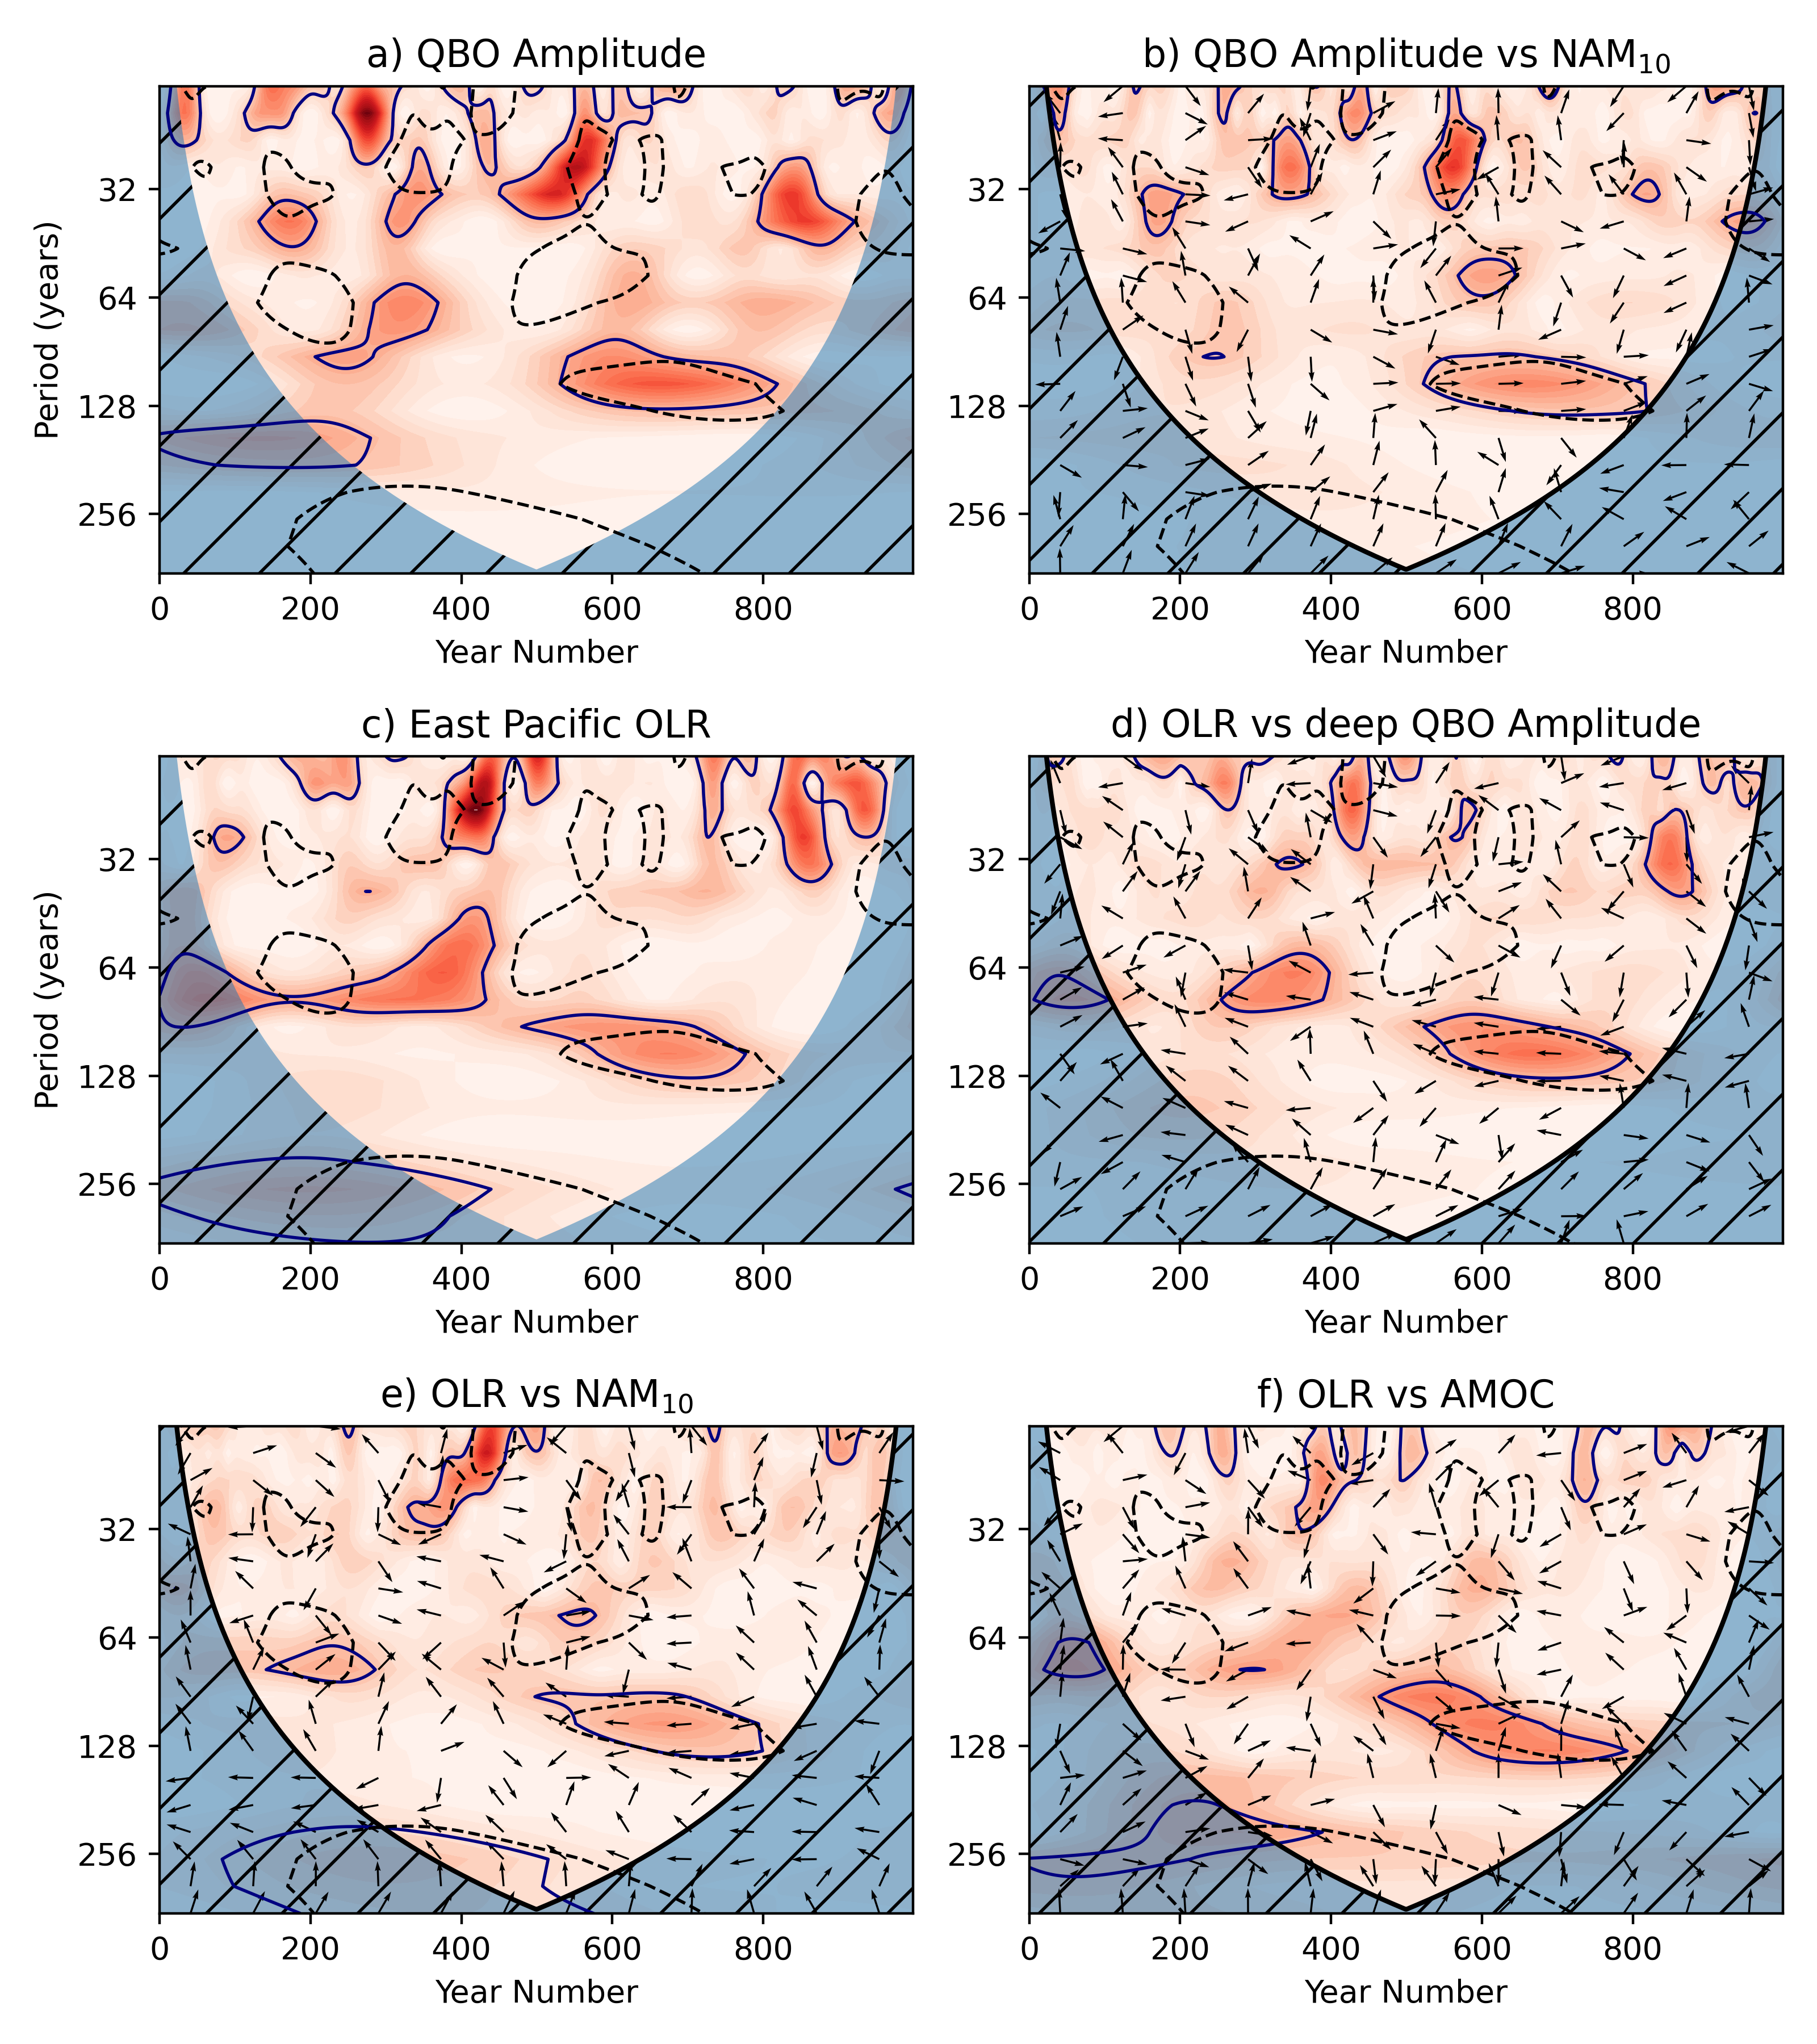
\includegraphics[width = 0.7\linewidth]{Figures/Figures-surface/OLR_wavelet.png}
\caption{\textbf(a): Wavelet power spectrum for the Sep-Nov deep QBO amplitude (see section \ref{sec:model_diagnostics_surface}). \textbf(b) cross power spectra between deep QBO Amplitude (Sep-Nov) and smoothed NAM$_{10}$ (Dec-Mar). \textbf(c): Wavelet power spectrum for the Sep-Nov  Area weighted average equatorial East Pacific OLR (see section \ref{sec:model_diagnostics_surface}). \textbf{d-f}: cross power spectra between combinations of East Pacific OLR, deep QBO Amplitude (both Sep-Nov means), AMOC at 50N (annual mean, all months) and NAM$_{10}$ (Dec-Mar) indices all smoothed with the same Gaussian filter as is used throughout ($\sigma$ = 2 years). Indices involved are indicated by sub-figure titles, shading indicates cross power with a colour scale the same as that seen in figures 6-8, dashed contours the 95\% confidence interval for the NAM$_{10}$ spectrum and arrows the relative phase angle between signals in the indices.}
\label{OLR_wavelet}
\end{center}
\end{figure}


\section{Contribution of the stratosphere to recent AMOC changes}
Our analysis of the UKESM simulation has identified co-variations between modes of variability in stratospheric circulation and the AMOC. Intervals in which the winter stratospheric polar vortex is consistently strong are, on average, followed by an extended negative anomaly in AMOC strength with a lag of approximately 15-20 years (figure \ref{AMOC_comp_NAM}f). Recent observations of the AMOC have shown a negative trend in circulation strength of approximately $-2.7 Sv$ between 2004 and 2012 \citep{smeedNorth2018} before a marginal recovery after 2012 \citep{smeedAtlantic2019}. Modelling studies have proposed a key role for anthropogenic forcing in AMOC slowdown over the 20th century and into the future \cite{liuOverlooked2017, bakkerFate2016, liuMechanisms2019} however, the magnitude of this contribution as well as others carries significant uncertainties. Furthermore, the results shown in the previous sections suggest the possibility that stratospheric variability has also contributed to the observed AMOC changes, in response to nearly a decade of strong vortex years in the 1990s followed by a sequence of years with a weak, disturbed vortex in the early 2000s \citep{pawsonCold1999, manneyRemarkable2005}. 

To assess the potential role of stratospheric variability figure \ref{ERA5_series} shows the NAM, AMOC and NAO indices for the interval 1979-2020 from the ERA5 and rapid array datasets. The NAM$_{10}$ index is characterised by an interval of strong vortex winters between 1988 and 1997 in which all but 2 winters exhibited a positive NAM$_{10}$. This interval also contains no SSWs \citep{pawsonCold1999}. This is followed by a run of winters between 1998 and 2005 which exhibit anomalously weak NAM$_{10}$ values \cite{manneyRemarkable2005}. The filtered NAM$_{10}$ index (red dashed line) reflects the presence of these intervals with a peak in positive values centred around 1995 followed by a negative extreme centred around 2003. The smoothed NAO (green dashed line) from the same dataset broadly reflects these variations in the NAM$_{10}$ with positive NAO extremes in the 1990s. The long-term envelope of the NAO does not remain positive for as long as the NAM, primarily due to the anomalous negative NAO in 1996 \citep{halpertClimate1997}. The presence of this anomalous negative NAO in 1996 and the absence of a clear NAO anomaly in the following year despite the presence of strong positive anomalies in the stratospheric NAM$_{10}$ is indicative of the fact that there are many other factors that influence the NAO in addition to the stratospheric influence. The AMOC strength at 26N estimated from the Rapid Array observations between 2005 and 2019 are also shown (blue curve) and shows a negative trend between 2005 and 2012 followed by a recovery from 2012 onwards consistent with \cite{smeedNorth2018} and \cite{smeedAtlantic2019}. 

\begin{figure}[h!]
\begin{center}
\noindent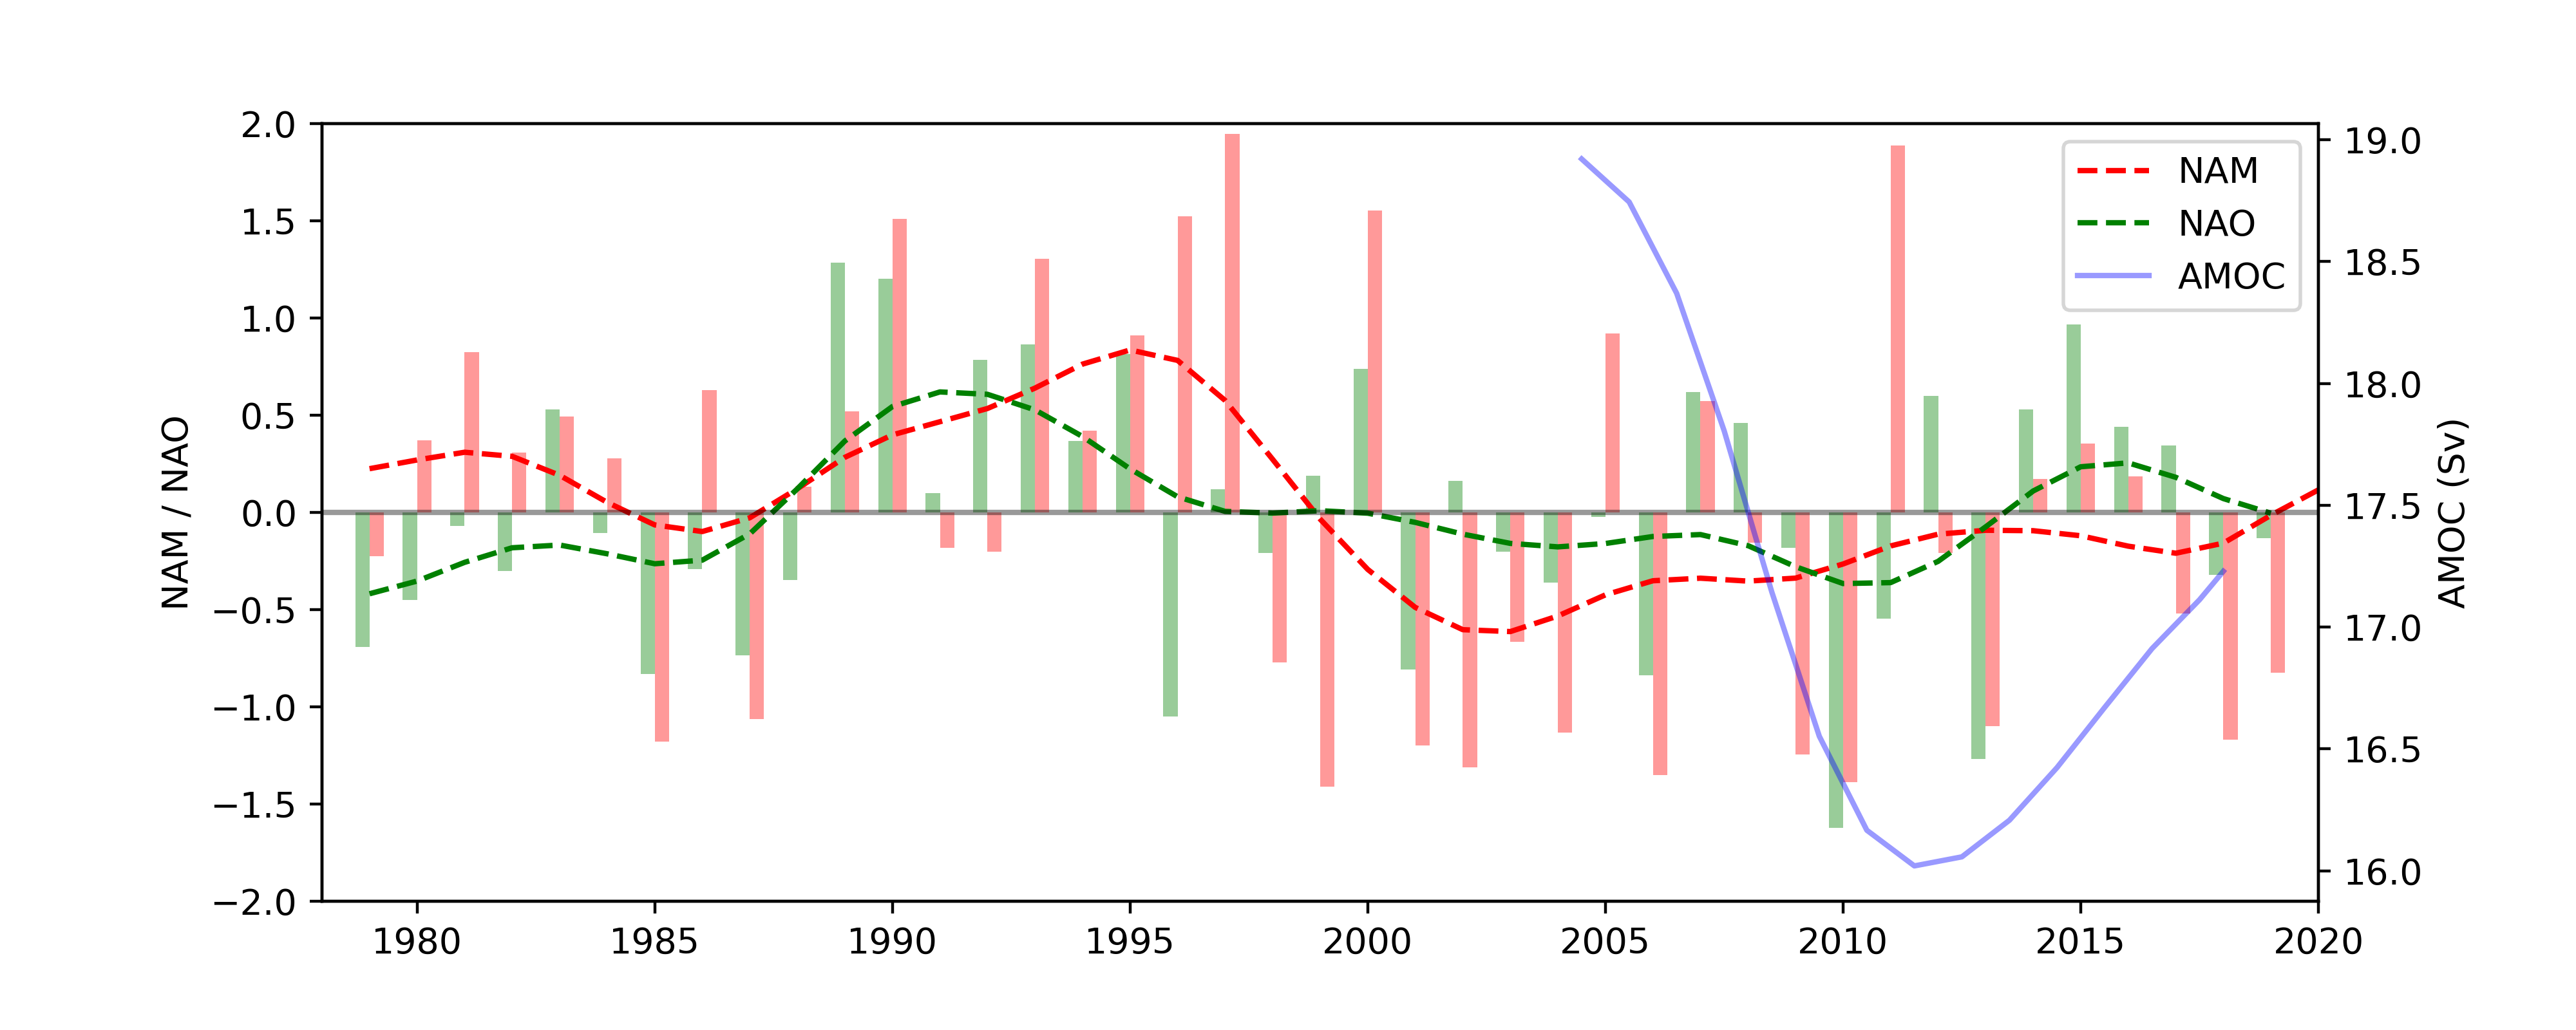
\includegraphics[width = 0.9\linewidth]{Figures/Figures-surface/ERA5_series_allf.png} \caption{Time series of the Dec-Mar NAO index (green bars), NAM$_{10}$ index (red bars) from the ERA5 dataset. Dashed lines correspond to indices shown by bars smoothed with a Gaussian filter ($\sigma$ = 2 years). Also included is the  AMOC timeseries at 26N from the rapid array dataset (blue) also smoothed with the same filter.}
\label{ERA5_series}
\end{center}
\end{figure}

The interval of observed consecutive strong NAM winters in the 1990s is anomalous in the reanalysis period although the available data record is rather short to allow a robust assessment. The amplitude and longevity of the observed anomaly is also large when compared to the UKESM simulation. Only 2 intervals in the simulation exhibit at least as many consecutive winters with strong (high NAM$_{10}$) conditions. These 2 intervals occur in the 300-400 year interval (centred around years 349 and 376) as shown in figure \ref{special_events}a. they exhibit a sequence of 10 and 14 consecutive Dec-Mar anomalously positive NAM$_{10}$ values respectively. This is reflected in the smoothed NAM$_{10}$ values (figure \ref{special_events}b) and these intervals represent the two of the three largest values of the filtered NAM$_{10}$ index (0.66 and 0.67). The corresponding smoothed AMOC index during these 2 intervals (blue curve in figure \ref{special_events}b) shows a positive AMOC response at lags of 2-3 years followed by a negative response at 17-20 years, in good agreement with figure \ref{AMOC_comp_NAM}f. The negative responses at 17-20 years following these 2 intervals of strong NAM$_{10}$ years are the 1st and 3rd greatest in magnitude compared to all other responses to persistent strong intervals. This is confirmed by figure 11b which shows the lagged AMOC response following all of the identified intervals with persistent positive NAM$_{10}$ anomalies (the two identified around 349 and 376 years are shown in black). 

To estimate the response amplitude of the AMOC to an interval of persistently strong vortex years figure \ref{special_events}d shows a scatter plot of the NAM$_{10}$ index evaluated at the centre of these intervals against the AMOC anomaly at 50N lagged by 17 years. This reveals a strong linear relationship ($r = -0.908$) between the size of the persistent vortex anomaly and the subsequent negative anomaly in the AMOC at 50N 17 years later. This correlation appears large and may indicate a strong relationship between stratospheric extreme and subsequent AMOC anomaly. However, given the relatively few anomalous vortex intervals selected (top 5 percentiles of the smoothed NAM$_{10}$) we must consider the probability that this correlation appears even if the lagged response in the timeseries occurs by chance. To assess this probability, we estimate a significance level for this value of $r = -0.908$ by assessing the probability such a value results if the phases in signals in the NAM$_{10}$ and AMOC are randomly assigned but the overall autocorrelation structure of each time-series is retained. We compare the $r$ value stated above with those produced from a set of synthetic NAM$_{10}$ series. These synthetic data are generated by Fourier transforming the smoothed NAM$_{10}$, randomly shuffling the Fourier phases and subsequently inverse Fourier transforming to generate a surrogate timeseries with the same Fourier power spectrum as the real data. Repeating this data generation and calculating the correlation between the magnitude of positive extremes in the surrogate NAM$_{10}$s and the 17 year lagged AMOC builds up a PDF for the $r$ value. This PDF of correlations is displayed in figure \ref{cors_stat_sigs}a (blue bars) along with the correlation generated by the real NAM$_{10}$ data (black vertical line). It shows that the $r$ value lies well outside the distribution of surrogate correlations indicating the high level of significance of the linear relationship.

A linear regression analysis on this data yields an estimated relationship between the variables which satisfies

\begin{equation}
AMOC'_{+17} = -6.54\space NAM max + 3.11,
\end{equation}

where $AMOC'_{+17}$ is the 17 year lagged AMOC anomaly at 50N and $NAM max$ is the magnitude of the positive extreme in smoothed NAM$_{10}$ at the centre of each interval. We can then use this relationship to predict the AMOC response to the observed sequence of strong vortex years in the 1990s. The maximum smoothed NAM$_{10}$ occurs in 1996 so the maximum AMOC response associated with the stratosphere would be 17 years later (2013) with amplitude of -0.89 Sv (figure \ref{special_events}d, purple point). This prediction suggests that $\sim$30\% percent of the observed reduction in AMOC strength  between 2005 and 2013 (0.89 Sv compared with 2.9 Sv in total) could be due to the presence of the persistent strong vortex winters that occurred during the 1990s. However, we acknowledge that the comparison between the interactions between the stratosphere and the AMOC at 50N in the model and 26N in observations may not be direct. Indeed, the modulation of the AMOC by the smoothed NAM$_{10}$ is less pronounced at 30N (figure \ref{AMOC_comp_NAM} and b) that at higher latitudes. Nevertheless, the Rapid Array dataset remains the most direct measurement of AMOC strength over the last 15 years and results from UKESM suggest a possible significant contribution towards trends over early the 21st century.  A similar analysis of the relationship between the magnitude of smoothed negative (weak) NAM$_{10}$ extremes and the lagged AMOC response (not shown) yields a significantly weaker relationship ($r = -0.21$). A similar significance analysis using surrogate time-series (see paragraph above) is shown in figure \ref{cors_stat_sigs}b, it shows that this $r$ value lies well within the PDF of surrogates suggesting the relationship may not be robust. This asymmetry in the relationship between extreme types is likely due to differences in dynamical behaviour associated with each extreme outlined in section \ref{persistent}. Namely that the surface signature of weak anomalies associated with SSWs are highly dependant on the timing of the SSW within the winter season while strong intervals generally exhibit strong vortex conditions throughout a winter.  

\begin{figure}[h!]
\begin{center}
\noindent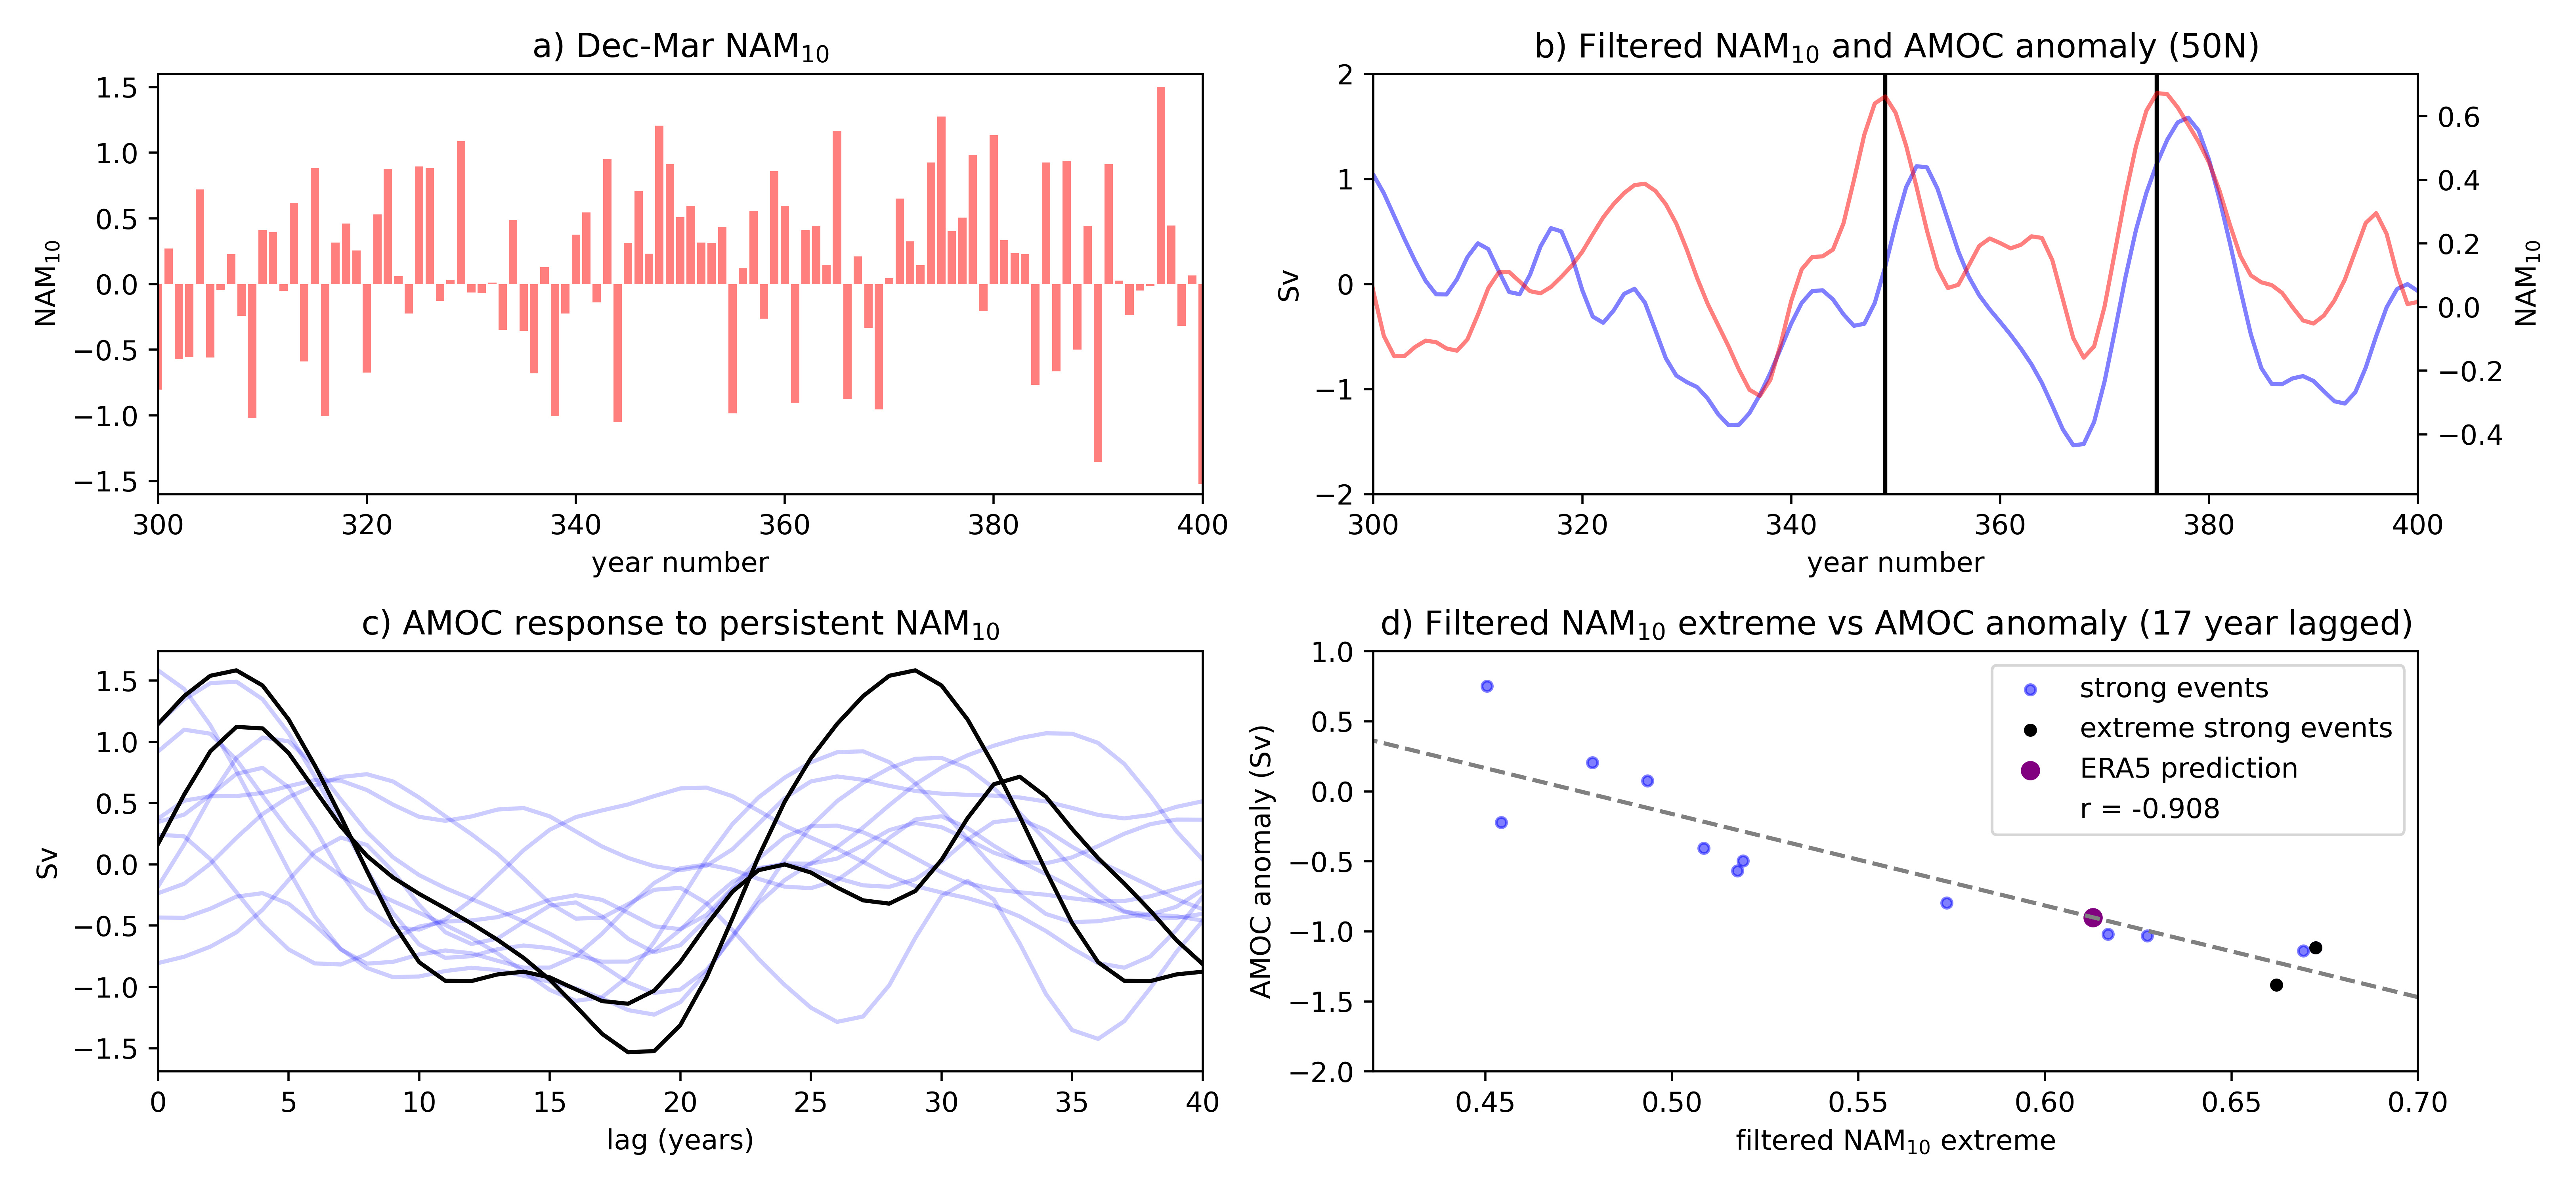
\includegraphics[width =\linewidth]{Figures/Figures-surface/AMOC_response_special_events.png} 
\caption{\textbf{a}: AMOC (blue) and NAM$_{10}$ (red) indices smoothed with the Gaussian filter ($\sigma$ = 2 years) between year numbers 300 and 400 of the UKESM simulation. \textbf{b}: AMOC at 50N associated with persistent strong NAM$_{10}$ intervals (light blue) and the intervals marked in \textbf{a} (black). \textbf{c}: Dec-Mar NAM$_{10}$ index from the UKESM simulation between year numbers 300 and 400. \textbf{d}: Scatter plot of filtered NAM$_{10}$ index values occurring at persistent strong NAM$_{10}$ intervals ($y$ axis) against AMOC anomalies at 50N lagged 17 years after persistent intervals' central year ($x$ axis). Blue points indicate persistent intervals and black dots represent the 2 intervals in the interval displayed in a. The dotted line represents the linear line of best fit for the points in black and blue. Also included is the 17 year lag AMOC anomaly predicted by projecting the regression coefficients used to construct the linear fit onto the maximum smoothed NAM$_{10}$ index in the ERA5 dataset (purple point).}
\label{special_events}
\end{center}
\end{figure}

\begin{center}
\begin{figure}[h!]
\noindent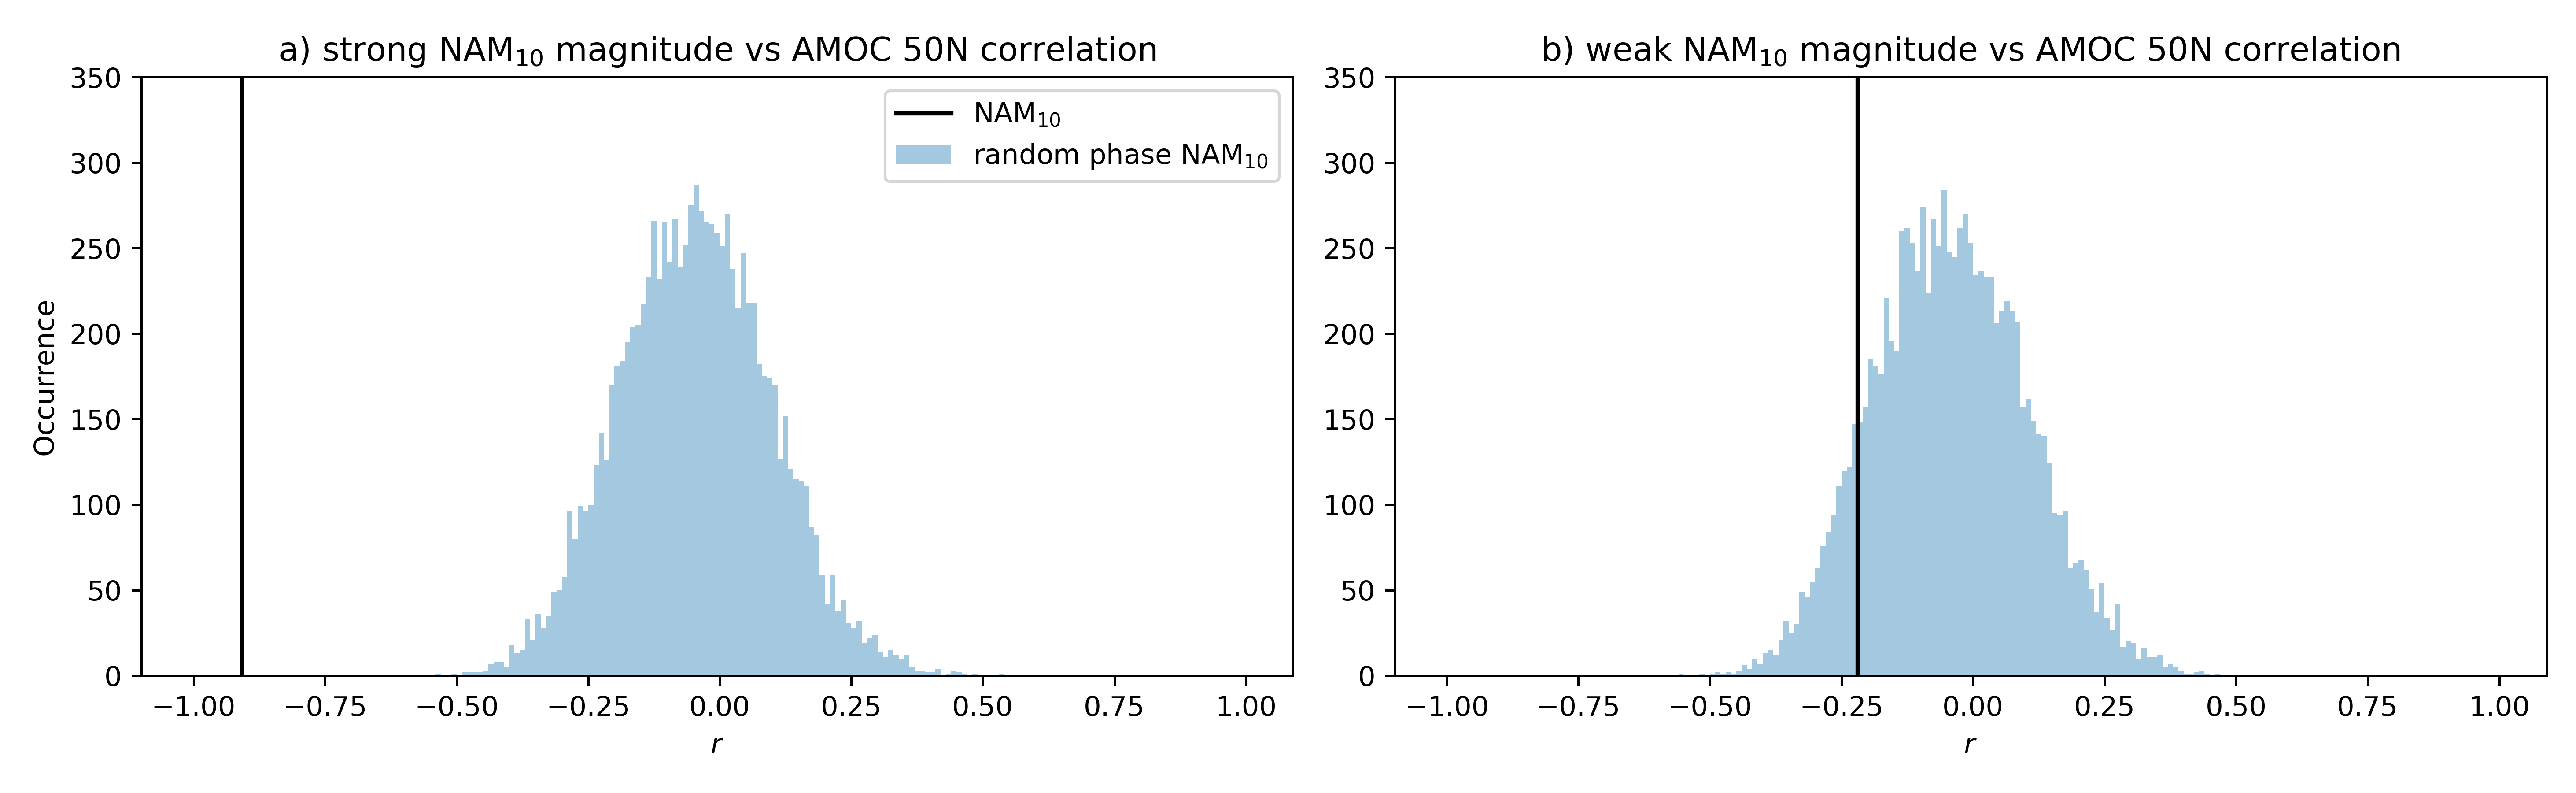
\includegraphics[width = \linewidth]{Figures/Figures-surface/correlation_stat_sigs.png}
\caption{Probability distribution functions (PDFs) for correlations between the magnitude of NAM$_{10}$ extreme positive (\textbf{a}) and negative (\textbf{b}) values from surrogate NAM$_{10}$ data and anomalies in the AMOC at 50N evaluated 17 years later. Each NAM$_{10}$ surrogate is generated by Fourier transforming the smoothed NAM$_{10}$ index, randomly shuffling the Fourier phases and inverse transforming. Each PDF is built with 10000 surrogates and the correlation between the NAM$_{10}$ extreme magnitude and 17 year lagged AMOC anomaly at 50N is shown by vertical black lines in both subfigures.}
\label{cors_stat_sigs}
\end{figure}
\end{center}

\section{Sensitivity to NAM thresholds and filtering}

- Our results are dervied from a stratosperic index which is highly processed. Both by smoothing and selecting extreme values to define intervals of anomalous behaviour. 

- This processing relies on choices of filtering kernel width (the parameter $\sigma$) as well as the threshold value to define an interval of persistent vortex behaviour. 

- so far, we have chosen these parameters in line with previous studies that utilise this metric \citep{reichlerStratospheric2012}

\begin{figure}[h!]
\begin{center}
\noindent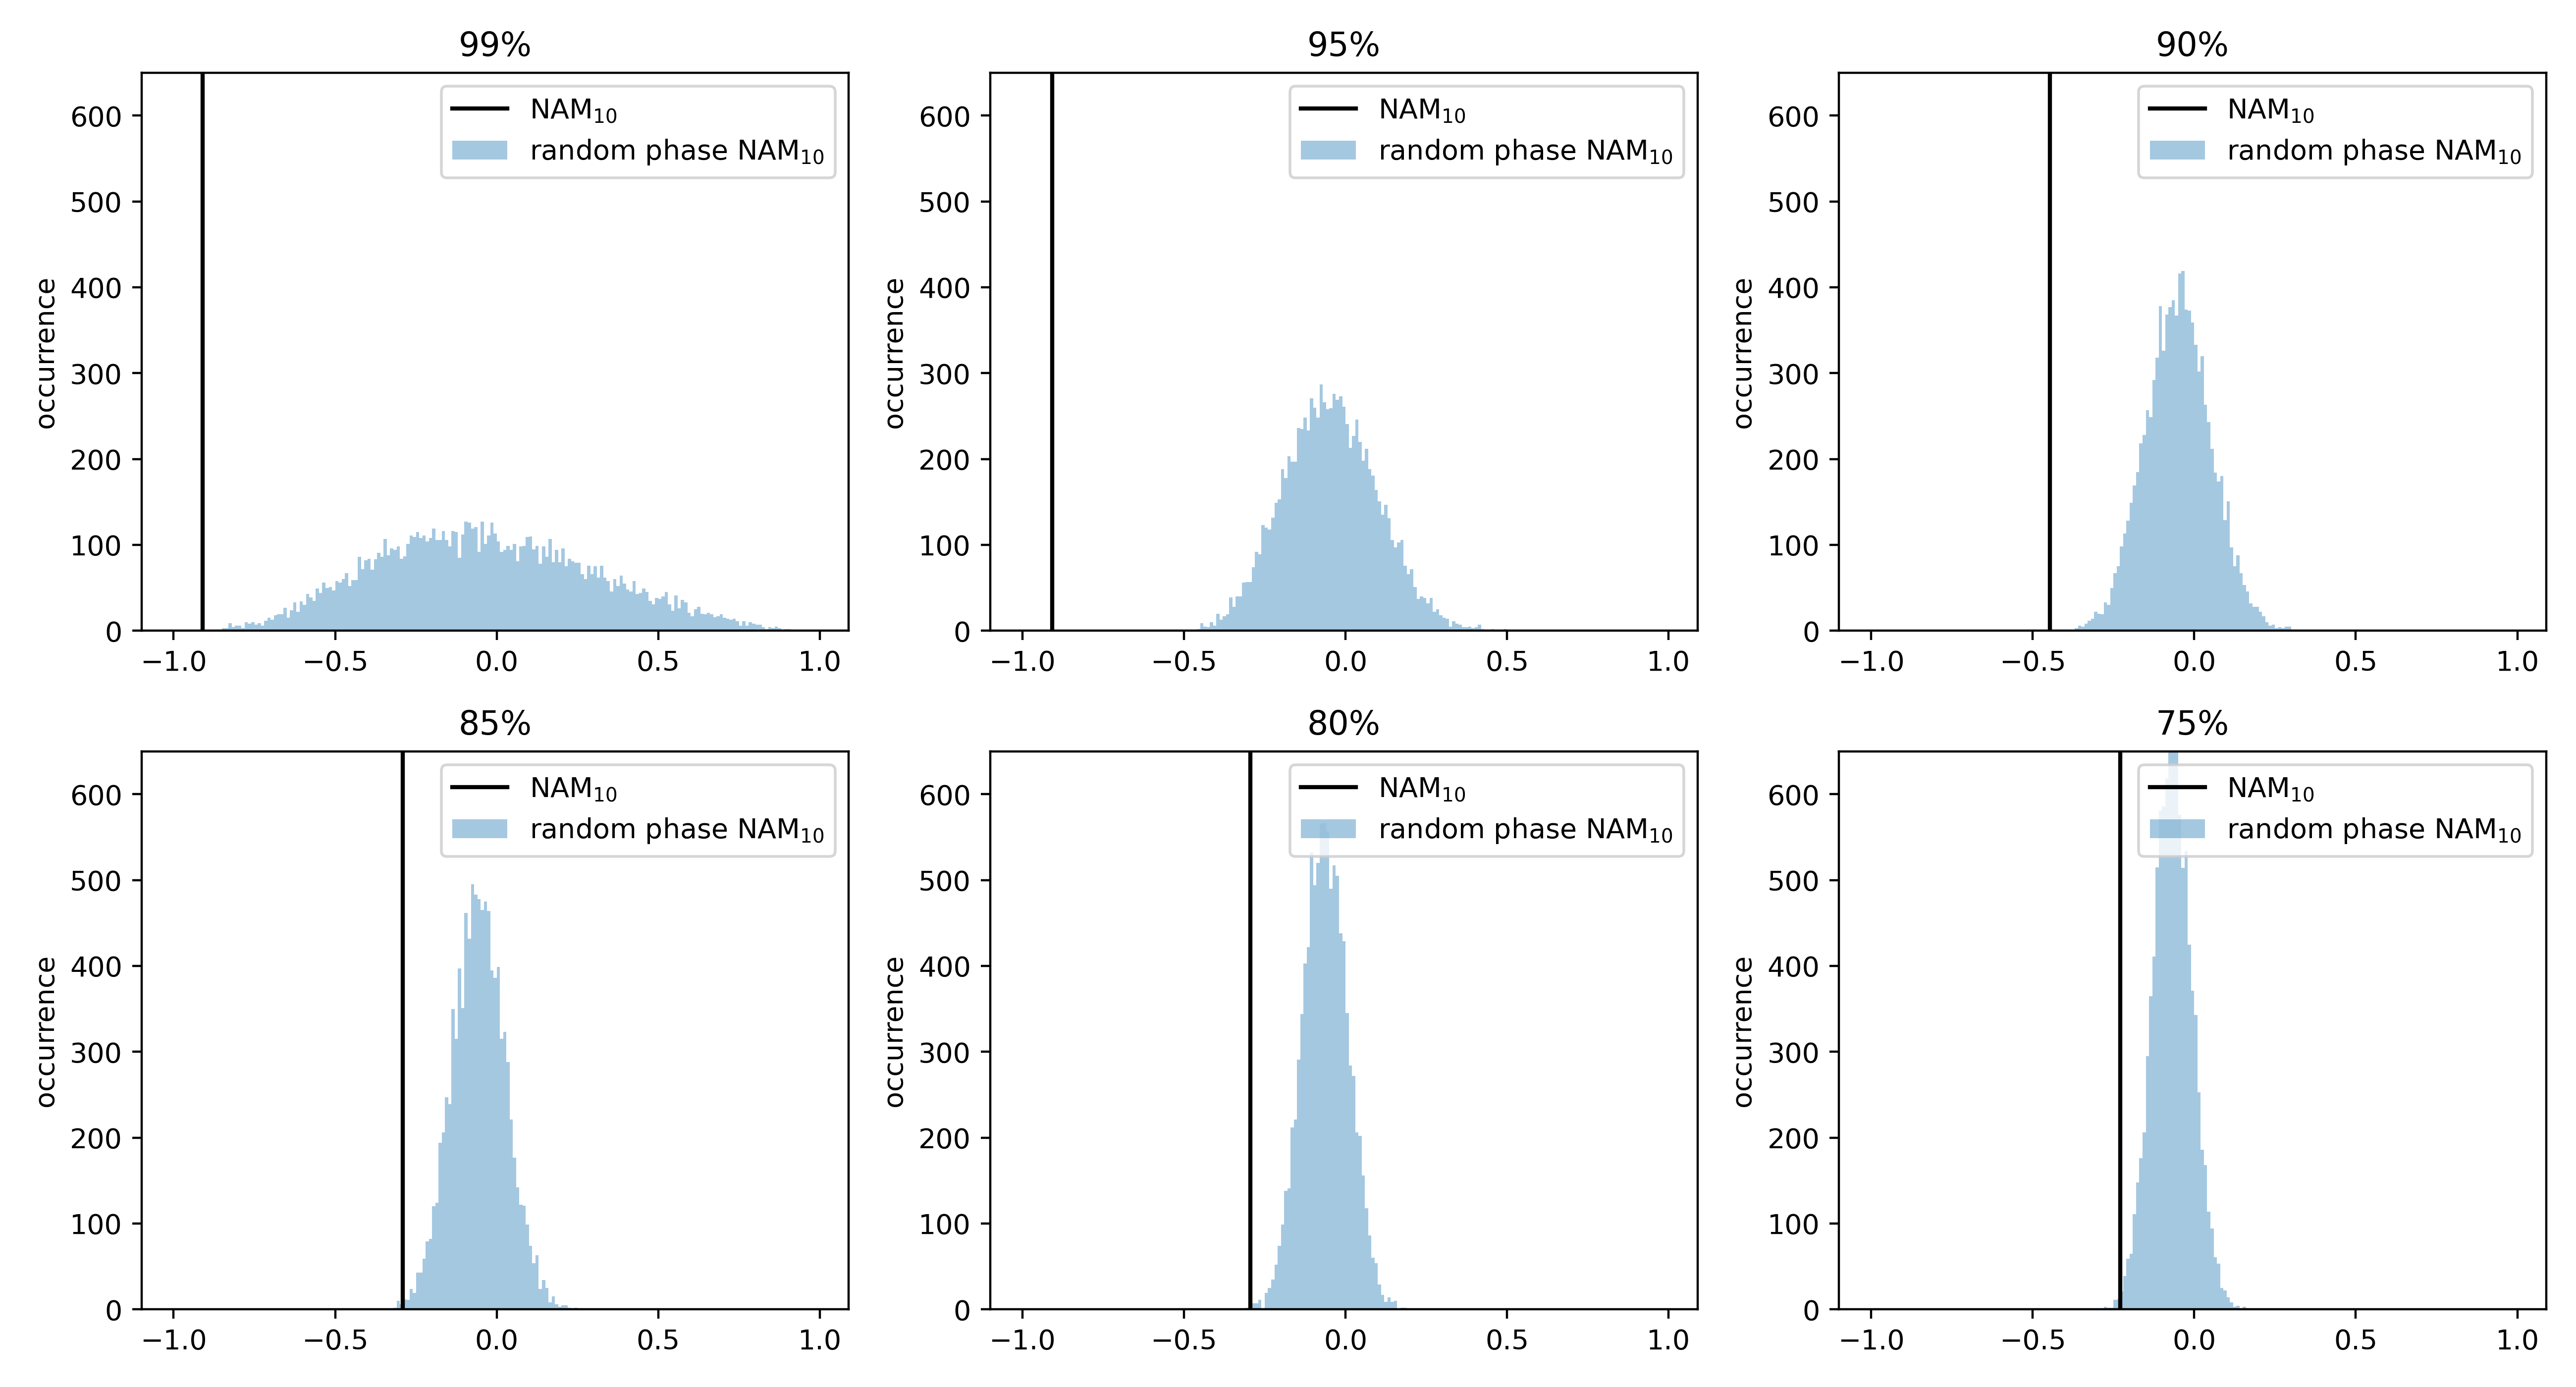
\includegraphics[width =\linewidth]{Figures/Figures-surface/bootstraps_different_threshold_strong.png} 
\caption{like figure \ref{cors_stat_sigs}a - Probability distribution functions (PDFs) for correlations between the magnitude of NAM$_{10}$ extreme positive (\textbf{a}) and negative (\textbf{b}) values from surrogate NAM$_{10}$ data and anomalies in the AMOC at 50N evaluated 17 years later. Each subfigure shows the PDF using a different threshold to define a strong NAM$_{10}$ interval. The title of each subfigure indicates the percentile threshold used to define a strong NAM$_{10}$ interval, blue bars indicate the PDF of surrogate correlations and black vertical lines indicate the real correlation between NAM$_{10}$ extremes and 17 year lagged AMOC anomalies.}
\label{different_thresh_strong}
\end{center}
\end{figure}

\begin{figure}[h!]
\begin{center}
\noindent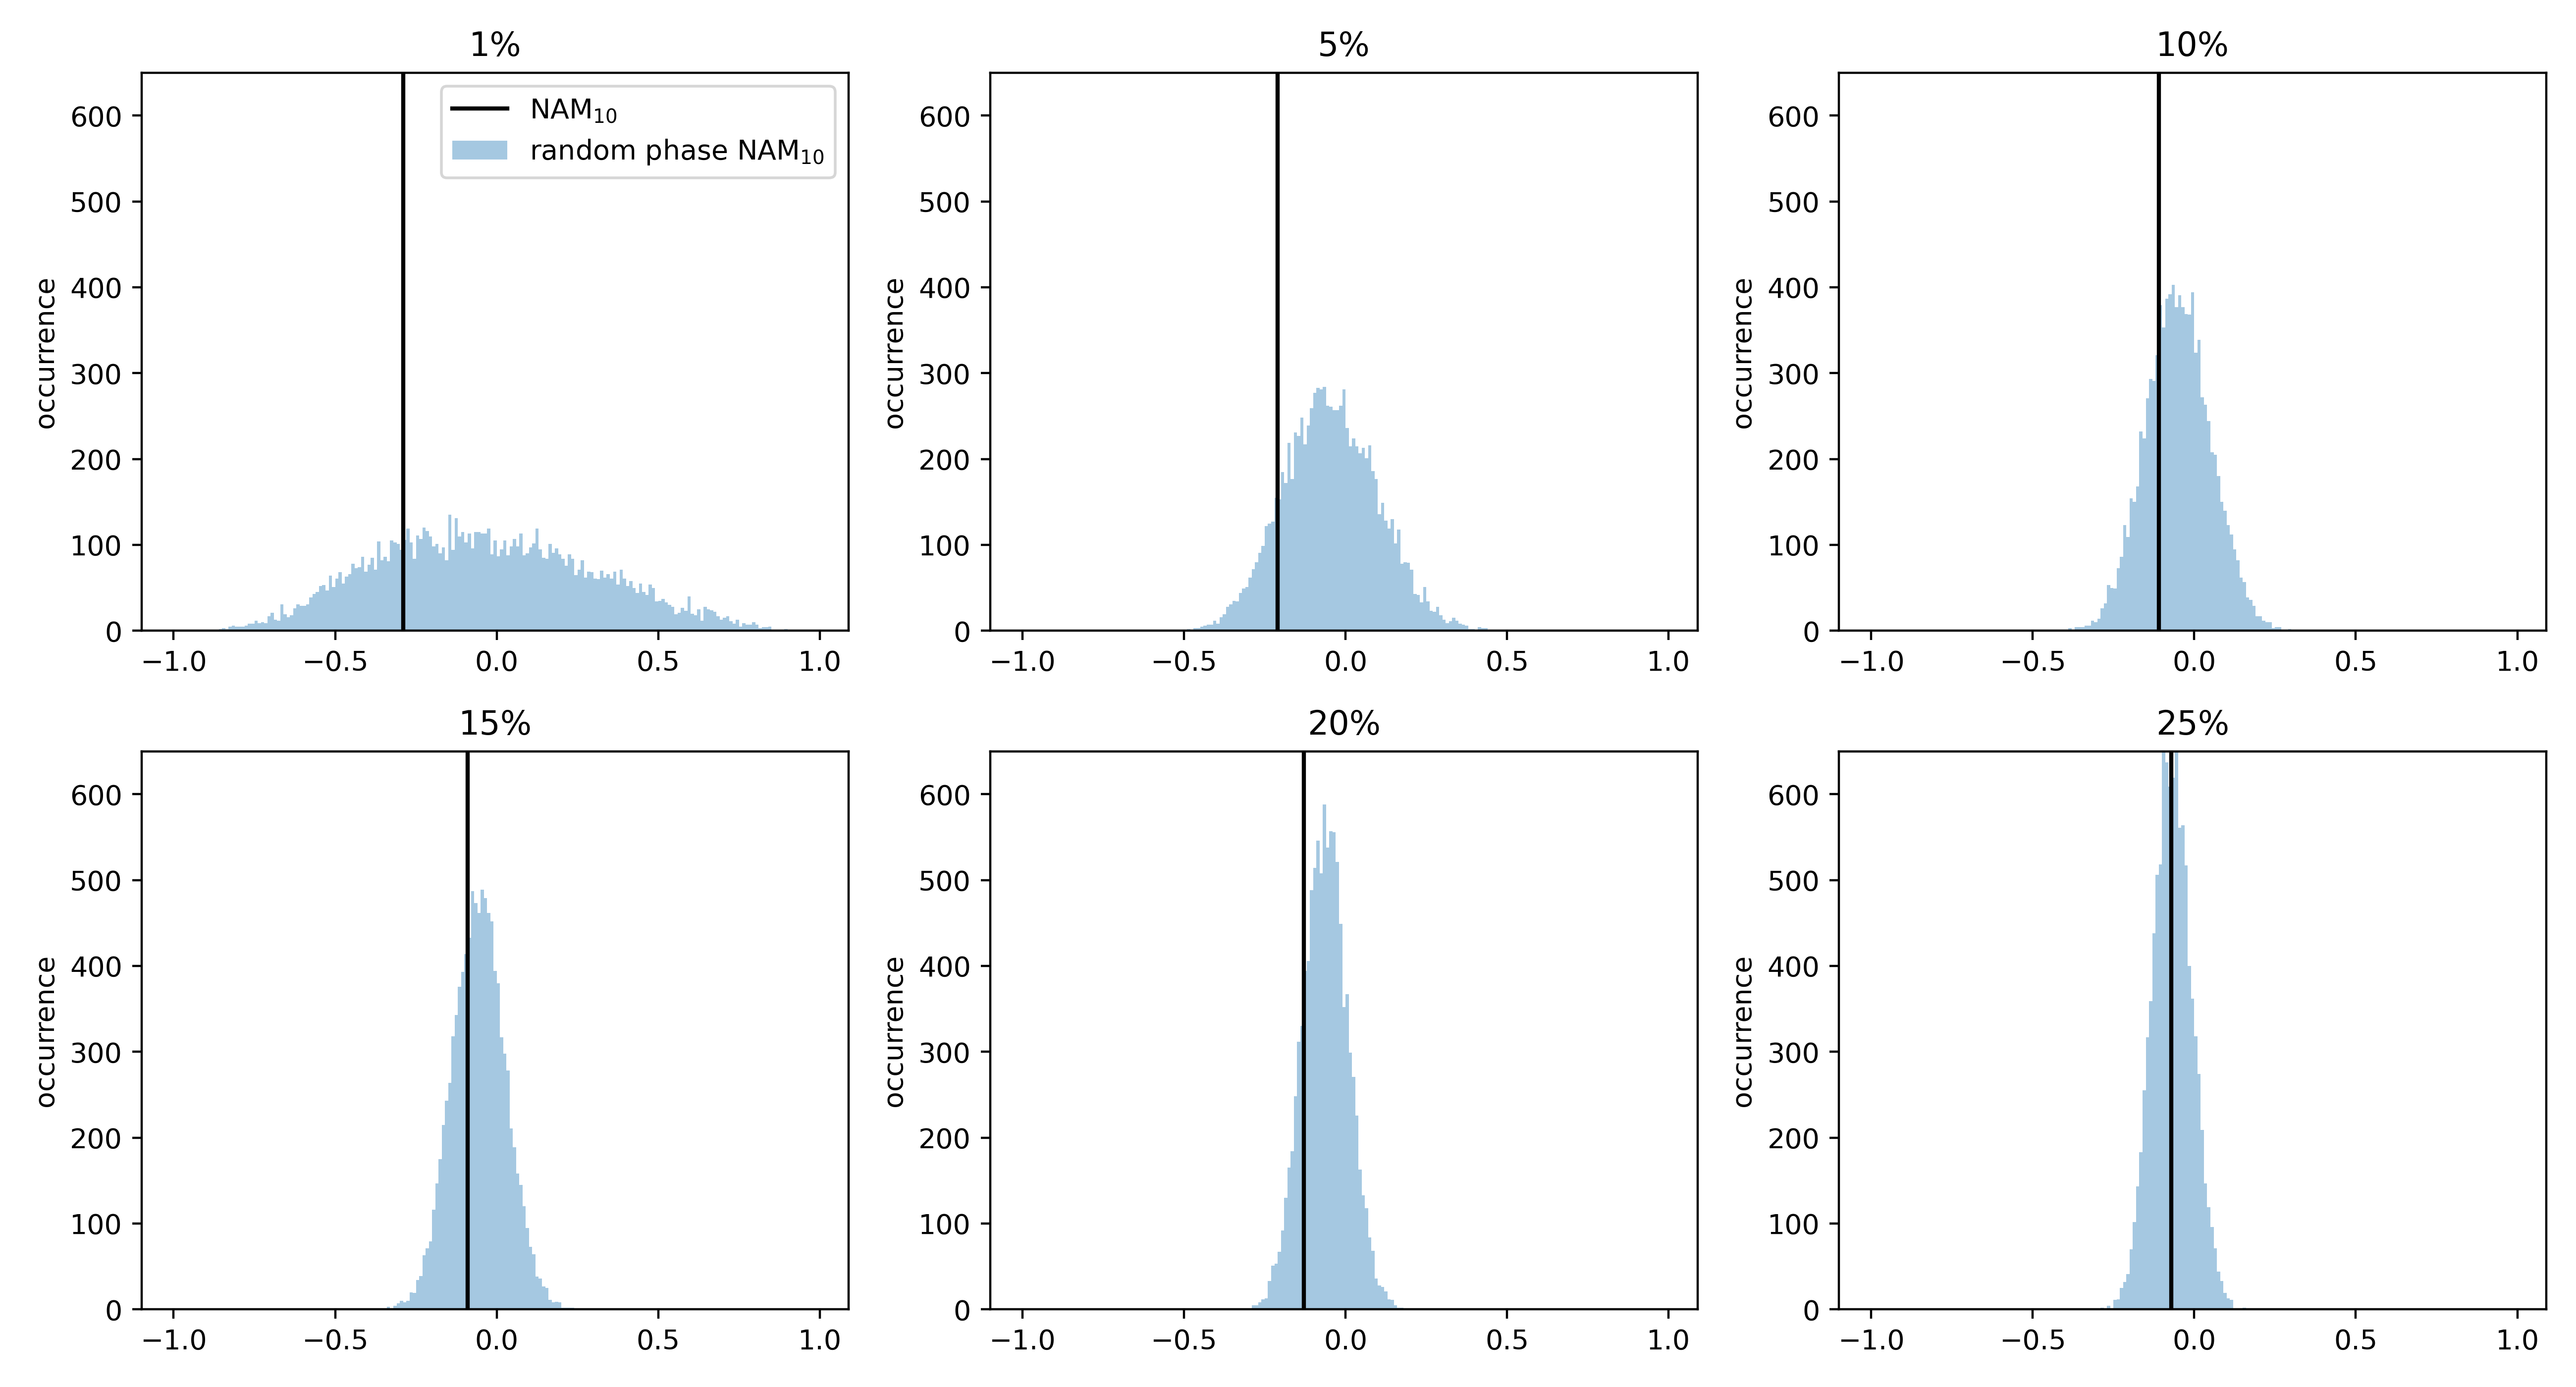
\includegraphics[width =\linewidth]{Figures/Figures-surface/bootstraps_different_threshold_weak.png} 
\caption{like figure \ref{different_thresh_strong} for weak NAM$_{10}$ intervals.}
\label{different_thresh_weak}
\end{center}
\end{figure}





%%% Local Variables:
%%% mode: latex
%%% TeX-master: "thesis"
%%% End:

\section{Summary and Discussion}

In this chapter we analyse the influence of persistent polar vortex extremes on surface and ocean circulation in a 1000 year pi-control simulation of UKESM. Persistent vortex anomalies are identified using a smoothed NAM$_{10}$ index which characterises intervals of approximately 6-8 years during which the NH winter vortex is anomalously strong (positive NAM$_{10}$ anomaly) or weak (negative NAM$_{10}$ anomaly). While the surface impacts of stratospheric extremes in individual winters (such as sudden stratospheric warmings) has received much attention \citep{baldwinStratospheric2001a, domeisenEstimating2019, charlton-perezInfluence2018a} the surface impacts of persistently anomalous winters has been less well studied and  teleconnections between the stratospheric vortex and ocean variability are not well characterised or understood. 

We examine the AMOC response to long-term variations in the stratospheric polar vortex using composite analysis of the AMOC strength following persistent anomalous NAM$_{10}$ intervals. We find oscillatory responses (figure \ref{NAO_AMOC_T_response}) from the NAO and the AMOC consistent with previous work  \citep{reichlerStratospheric2012}. We propose that this behaviour is due to a combination of effects. Firstly, resonant oscillatory signals in the NAM$_{10}$ and the AMOC which involve the ocean's natural modes of oscillation being amplified due to integrated forcing from the atmosphere (originating from the vortex) varying on a similar timescale. Secondly, through feedbacks between the NAO, which is initially perturbed by the NAM, and the AMOC in which the NAO signal is able to penetrate into the deep ocean thermocline which subsequently forces and then responds to the AMOC. This induces a change in the NAO phase which damps the AMOC response.

We also find that different types of persistent vortex intervals are associated with different AMOC patterns in the simulation. Namely, strong intervals lead to oscillatory responses of near 30 year periods with peaks in the NAM$_{10}$ leading those in the AMOC by approximately 2-4 years. Meanwhile, weak intervals associate with longer timescale (50-100 years) variations in the ocean with the extremes in the AMOC appearing both before and after peaks in the persistent NAM. We aim to understand these differences by considering the vortex behaviour under strong and weak conditions, i.e. weak winters will only influence the surface once an SSW occurs, while strong winters act through the whole season. Whilst this represents an asymmetric forcing, just how this accounts for different AMOC response timescales is unclear. We additionally found prominent signal non-stationarities across multiple timescales in the AMOC, NAO and NAM$_{10}$. Wavelet analysis reveals 3 intervals during which 30, 50 and 90 year periodic behaviour is present in the NAM$_{10}$ and AMOC, 2 of which (those at 50 and 30 year periods) also feature similar signals in the NAO. We therefore propose that the composite response patterns seen in this analysis are the superposition of contributions from intervals exhibiting different timescale behaviour. The distribution of different persistent vortex interval types relative to these intervals therefore accounts for the different AMOC behaviour associated with them: a large proportion of strong intervals are situated within the 30 year timescale interval while a higher proportion of weak intervals occur during the 50 and 90 year timescale intervals. On the 90 year timescale we show that signals in the vortex are associated with similar variations in tropical east Pacific deep convection and QBO amplitude. The AMOC also appears to co-vary with the rate of change of such tropical convection also with 90 year periods completing a possible novel AMOC pathway to influence the strength of the vortex.

We subsequently assess the relationship between the magnitude of the strong persistent NAM$_{10}$ intervals and the resulting AMOC anomalies. This analysis suggests that the magnitude of filtered NAM$_{10}$ extremes, which captures both the strength of anomalous vortex behaviour as well as the persistence of the same type of behaviour in an approximately 6-8 year window, is directly proportional to the AMOC anomaly 17 years later. This relationship is shown to display a remarkable degree of correlation ($r = 0.908$). We finally use this relationship to estimate the contribution of the persistent strong interval of the 1990s, which appears in observations, on recent AMOC trends. This method predicts a -0.89Sv anomaly in the AMOC due to the due to persistent strong vortex behaviour during the 1990s.

This final finding is a striking, novel result: -0.89Sv represents nearly 30\% of the total decrease in AMOC transport between 2005 and 2013 which has been primarily attributed to anthropogenic forcing factors \citep{caesarObserved2018, caesarCurrent2021}. In contrast, NH vortex variability is largely regarded as a mode of internal variability within the climate system - there is no consensus amongst GCMs as to the response from the vortex to anthropogenic forcings \citep{ayarzaguenaUncertainty2020}. As a result, our findings may indicate a significant role of internally generated signals in recent observations of the AMOC. However, The result relies on a number of key assumptions: First, we assume that the relationship between strong persistent NAM$_{10}$ intervals and the AMOC holds in the real climate system. As the connection proposed is not well explored in previous literature, there is limited analysis on the ability of GCM's to represent vortex-AMOC interactions (\cite{reichlerStratospheric2012} showed some interaction in CMIP5 models). However, some studies report that GCMs under-represent the influence of SSW events on the jet, NAO and surface temperatures in the form of the so called "signal to noise" problem in which stratospheric signals in GCMs fail to emerge above noise in tropospheric variability \citep{scaifeSignaltonoise2018}. Such an issue does not appear to emerge in UKESM however as a clear NAO signal is apparent up to 3 months following events (figure \ref{surface_comp_all} top row) indicating that reasonable connection between the stratosphere and the surface is present in the simulation and that connections with the AMOC may also be realistic. 

Second, the interaction between persistent vortex intervals and the AMOC in the simulation appears to be heavily weighted towards the interval in which 30 year timescale variations in both modes dominate. This variability is a non-stationary feature which persists for approximately 70-100 years of the 1000 year simulation. We therefore assume that such variability is also realistic within the observational record and the validity of this assumption may rely on whether such an interval is present in the real climate system. If we consider the pi-control simulation as a realisation of the real climate system over an arbitrary 1000 year interval, we can estimate the probability of the emergence of such intervals as 0.07-0.10 as 30 year variations appeared for 70-100 years in the 1000 year simulation. This suggests 30 year timescale variations are most likely not present in the observations. However, the linear relationship between NAM$_{10}$ extreme magnitude and AMOC anomaly is established from the whole simulation suggesting that connection is not solely confined to 30 year variations despite the heavy weighting towards intervals exhibiting this frequency variability.

Overall, results from this chapter suggest a novel, non-stationary interaction between the vortex and Atlantic circulation as well as suggest a possible key role for the stratosphere in recent AMOC observations. Key limitations to the analysis presented here as well as further work following on from this study is explored in section \ref{sec:limitations}.







\chapter{The role of vertical structure in QBO teleconnections}
\label{cha:deepQBO}

\section{Introduction}
\label{sec:deepQBO-introduction}
The QBO is typically defined by the equatorial ZMZW at a single level in the mid-stratosphere. The 50 hPa level is usually used for NH observational studies \citep{Baldwin2001, Baldwin98} but some studies have also noted the importance of characterising the vertical structure of the QBO \citep{Fraedrih1993, Wallace1993,  Baldwin98,  Dunkerton2017, graySurface2018, andrewsObserved2019}. In an observational-based study \cite{graySurface2018} find an enhanced association between the QBO and polar vortex when a metric incorporating the vertical coherence of equatorial winds via empirical orthogonal functions is utilised \citep{verena2016a}. In a model-based study \cite{andrewsObserved2019} introduce a similar but simpler methodology by defining the QBO as the average ZMZW between two vertical levels, which preferentially selects time intervals that display a vertically coherent QBO phase between the specified levels. The same study reports enhanced responses to the QBO from the NAO and Arctic Oscillation (AO) when such vertically integrated metrics are used to define QBO phase compared to a single level definition. While these studies highlight statistical associations between vertical QBO metrics and the vortex, the importance of vertical coherence in HT strength has not been tested explicitly. Furthermore, influence mechanisms are not well understood. 


\section{Model Configuration}

To explicitly test the effect of QBO vertical coherence on teleconnections we utilise a set of custom designed simulations which utilises a modified version of the UKESM GCM analysed in chapters 3 and 4. As with the pi-control simulation examined so far, the model component for the atmosphere is GA7.1, GHG concentrations are set to 1850 levels (see section \ref{sec:model_config}) and volcanic eruptions are absent (however a constant background volcanic aerosol level is imposed). The primary difference between the pi-control and the configuration utilised here is the experiments run with no coupled Ocean component. Instead, SSTs are prescribed using a seasonally invariant climatological field obtained from an interval of the the pi-control (year numbers 96-126). Sea Ice extents are also prescribed to climatological values using the same interval of the pi-control and full documentation for this type of timeslice experiment is provided in \cite{oconnorAssessment2021}. All simulations are initialised using conditions from the start of the 30 year interval of the pi-control used to calculate SST and SI climatologies (year number 96). We choose to impose SST and sea ice conditions in our experiments as this removes contributions to atmospheric circulation from interannual to decadal surface modes of variability such as ENSO and the AL. This in turn isolates the effect of the QBO further as any differences in QBO-vortex and QBO-surface interactions across the simulations are not due to coupling with SSTs and other surface boundary conditions.  %Analysis chapters 4 and 5 showed that this year does not lie in an interval in which the QBO or the vortex exhibits significant multi-decadal oscillations. As a result, the initial conditions for the simulation are less likely samples the QBO and vortex in a randomly chosen state.

\section*{Nudging}
In order to impose the vertical structure of the QBO in our sensitivity experiments we employ a method to constrain atmospheric conditions in a GCM simulation known as nudging. In this method, an atmospheric quantity, $Y$, is constrained via Newtonian-relaxation which pushes the model state for $Y$ towards some imposed value at each model timestep such that

\begin{equation} \label{eq:nudging}
\Delta Y = G \Delta t (Y_{imposed} - Y_{model}), 
\end{equation}

where $Y_{imposed}$ is the state of $Y$ from the imposed field, $Y_{model}$ is the value of $Y$ the model has evolved to since the last timestep (when it was last nudged), $\Delta Y$ is the change in $Y$ applied by the nudging scheme and $G$ is the relaxation parameter. $G$ is a measure of the strength of the relaxation towards $Y_{imposed}$ at each timestep and can also be expressed as $G = \frac{1}{\tau}$ where $\tau$ is known as the relaxation timescale. When choosing the relaxation timescale, a balance is required between constraining the model sufficiently to the imposed state (I.E. a short enough $\tau$ such that the model's $Y$ avoids evolving freely) and avoiding the introduction of large gradients (a large enough $\tau$ to avoid model instability). The MetOffice Unified model, of which the model configurations presented here are a part, typically uses a relaxation timescale of 6 hours at all vertical levels. This has been shown to produce good quality nudging results in a range of studies employing such a method despite the different radiative timescales present across atmospheric levels (Brown et al. 2020). In our experiments we to nudge the zonal wind, $U$, towards an idealised version of the QBO wind fields expressed as 

\begin{equation} \label{eq:imposed_U}
U_{qbo}(t, z) = F(z) sin(\frac{2\pi (t + zs)}{period}),
\end{equation}

Where $s$ is a parameter which sets the rate of phase shift with descending height. We set $s$ to xxxx and the For the deep QBO experiment (that which displays a high degree of vertical coherence) and xxx for the shallow QBO to ensure a large phase shift with height (and therefore less vertical coherence). We choose the period of the QBO in both experiments to be xxx months for consistency with the QBO period exhibited in the UKESM pi-control. $F(z)$ is a momentum forcing vertical profile (seen in figure xxx) applied to reproduce the variation in magnitude of the QBO with height. Following the methodology of Pascoe et al., we use an $F(z)$ which takes the form of a Weibull function given by

\begin{equation} \label{eq:vertical_profile}
F(z) = R_D \frac{1}{\gamma \beta^\alpha}  Z_D^{\alpha-1}  e^{-Z_D/\beta},
\end{equation}

where the parameters are set to $\alpha = 3.5, \beta = 0.27, \gamma = 3.2335, R_D = 40.0 ms^{-1}, Z_{D} = (z - 15)/20$. The idealised time-height QBO profiles generated for both experiments are shown in figure xxxxa, they highlight the differences between idealised QBOs: The deep QBO winds exhibits the same sign of wind throughout the middle atmosphere for the majority of the series while the shallow QBO show different phases between the upper and middle stratosphere. In both experiments we apply the relaxation in equation \ref{eq:nudging} towards the corresponding QBO winds over the set of atmospheric levels approximately corresponding to the pressure level range xx-xxhPa and the latitudinal range xx-xx. The relaxation is applied at all longitudes. At the boundary between of these ranges we apply a tapered version of the relaxation with a value of that parameter $G$ that decreases linearly with increased distance from the relaxation region. This tapering is applied on the 2 atmospheric levels at the bottom and top of the vertical region and 5$^\circ$ either side of the latitudinal region. This tapering is applied to avoid introducing large vertical and latitudinal gradients in zonal wind and prevent potential model instability. 

\begin{figure}[h!]
\begin{center}
\noindent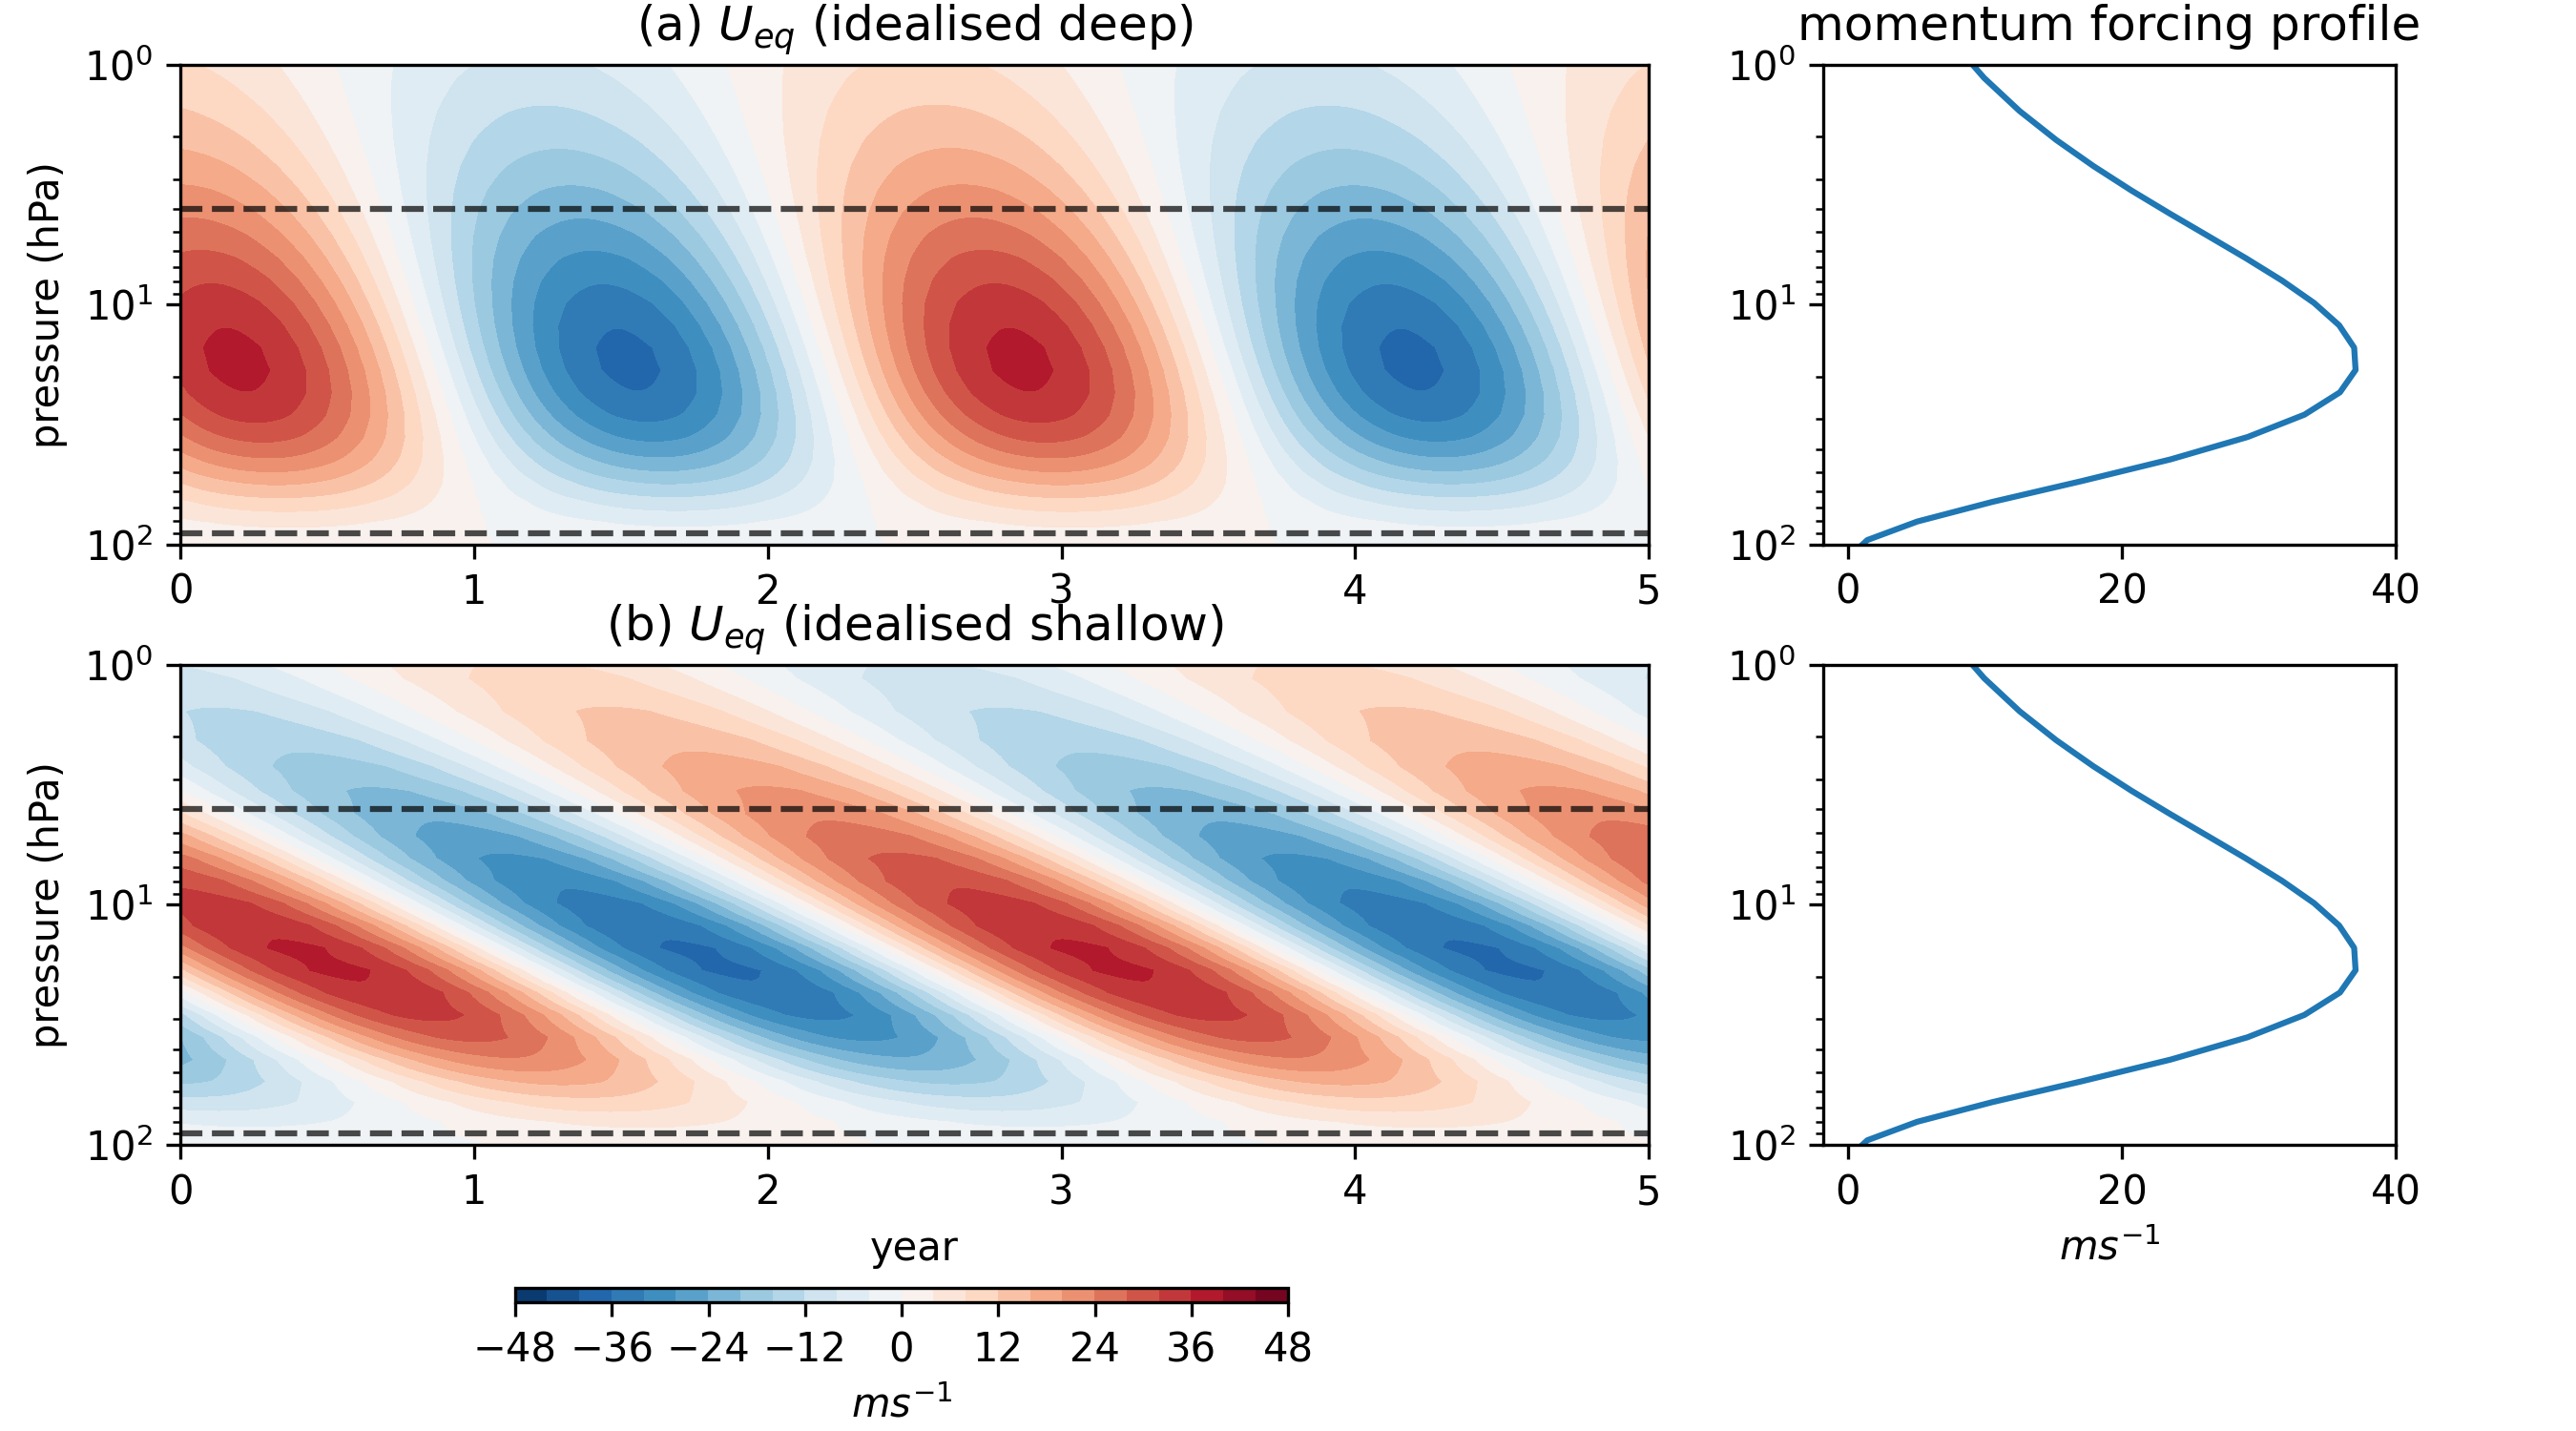
\includegraphics[width = \linewidth]{Figures/Figures-deepQBO/Idealised_QBO_features.png}
\caption[Idealised QBO winds used for nudging experiments]{Sample time-series of idealised equatorial ZMZW and associated momentum forcing profile for the deep (\textbf{a} and \text{b} respectively) and shallow (\textbf{c} and \textbf{d} respectively) QBO experiments. Horizontal dashed lines on (a) and (c) denote the xxhPa and 90hPa pressure levels between which we implement nudging towards the idealised wind in each experiment.}
\label{fig:Idealised_QBO_samples}
\end{center}
\end{figure}


\section{Results}
\subsection{QBO Characteristics}
We first analyse the equatorial winds in each experiment and verify if the implementation of nudging has resulted in realistic ZMZW profiles. Figure \ref{experiment_QBO_samples} shows the equatorial winds that results from implementing QBO nudging between the xxhPa and xxhPa levels. These winds reflect the key features of the idealised winds (figure \ref{fig:Idealised_QBO_samples}a and c) - the deep experiment exhibits vertical coherence in the middle stratosphere while the shallow simulation shows opposite phases of the QBO in the upper and lower stratosphere. This indicates that our selection of nudging timescale, $\tau$ = 6 hours, is suitable to fix the state of the QBO in each experiment. The period of ZMZW variations in the middle stratosphere (90-xxhPa) is also close to the value specified by the idealised winds ($\sim$32 months). Both experiments also exhibit spectral power in equatorial winds  corresponding to a period of approximately 6 months which indicate the presence of an SAO variation (see section \ref{sec:equatorial_strat}) in the simulations. This SAO variation is also visible in the full wind field (figure \ref{fig:experiment_QBOs}a and c) and the magnitude of winds in the deep experiment appear significantly larger than the shallow experiment. This difference is explored in closer detail in the following section. Climatological differences in ZMZW are also apparent across the experiments. Figure \ref{fig:climatologies_experim} shows latitude height profiles for winter months (Dec-Feb). The largest discrepacies across the simulations are situated near the 10hPa level where the deep experiment exhibits greater westerly amplitude winds

- differences at the nudging boundary over the equator

- large climatological differences in SAO region, likely due to filtered waves

- vortex climatology differences - deep QBO exhibits stronger vortex. 

\begin{figure}[h!]
\begin{center}
\noindent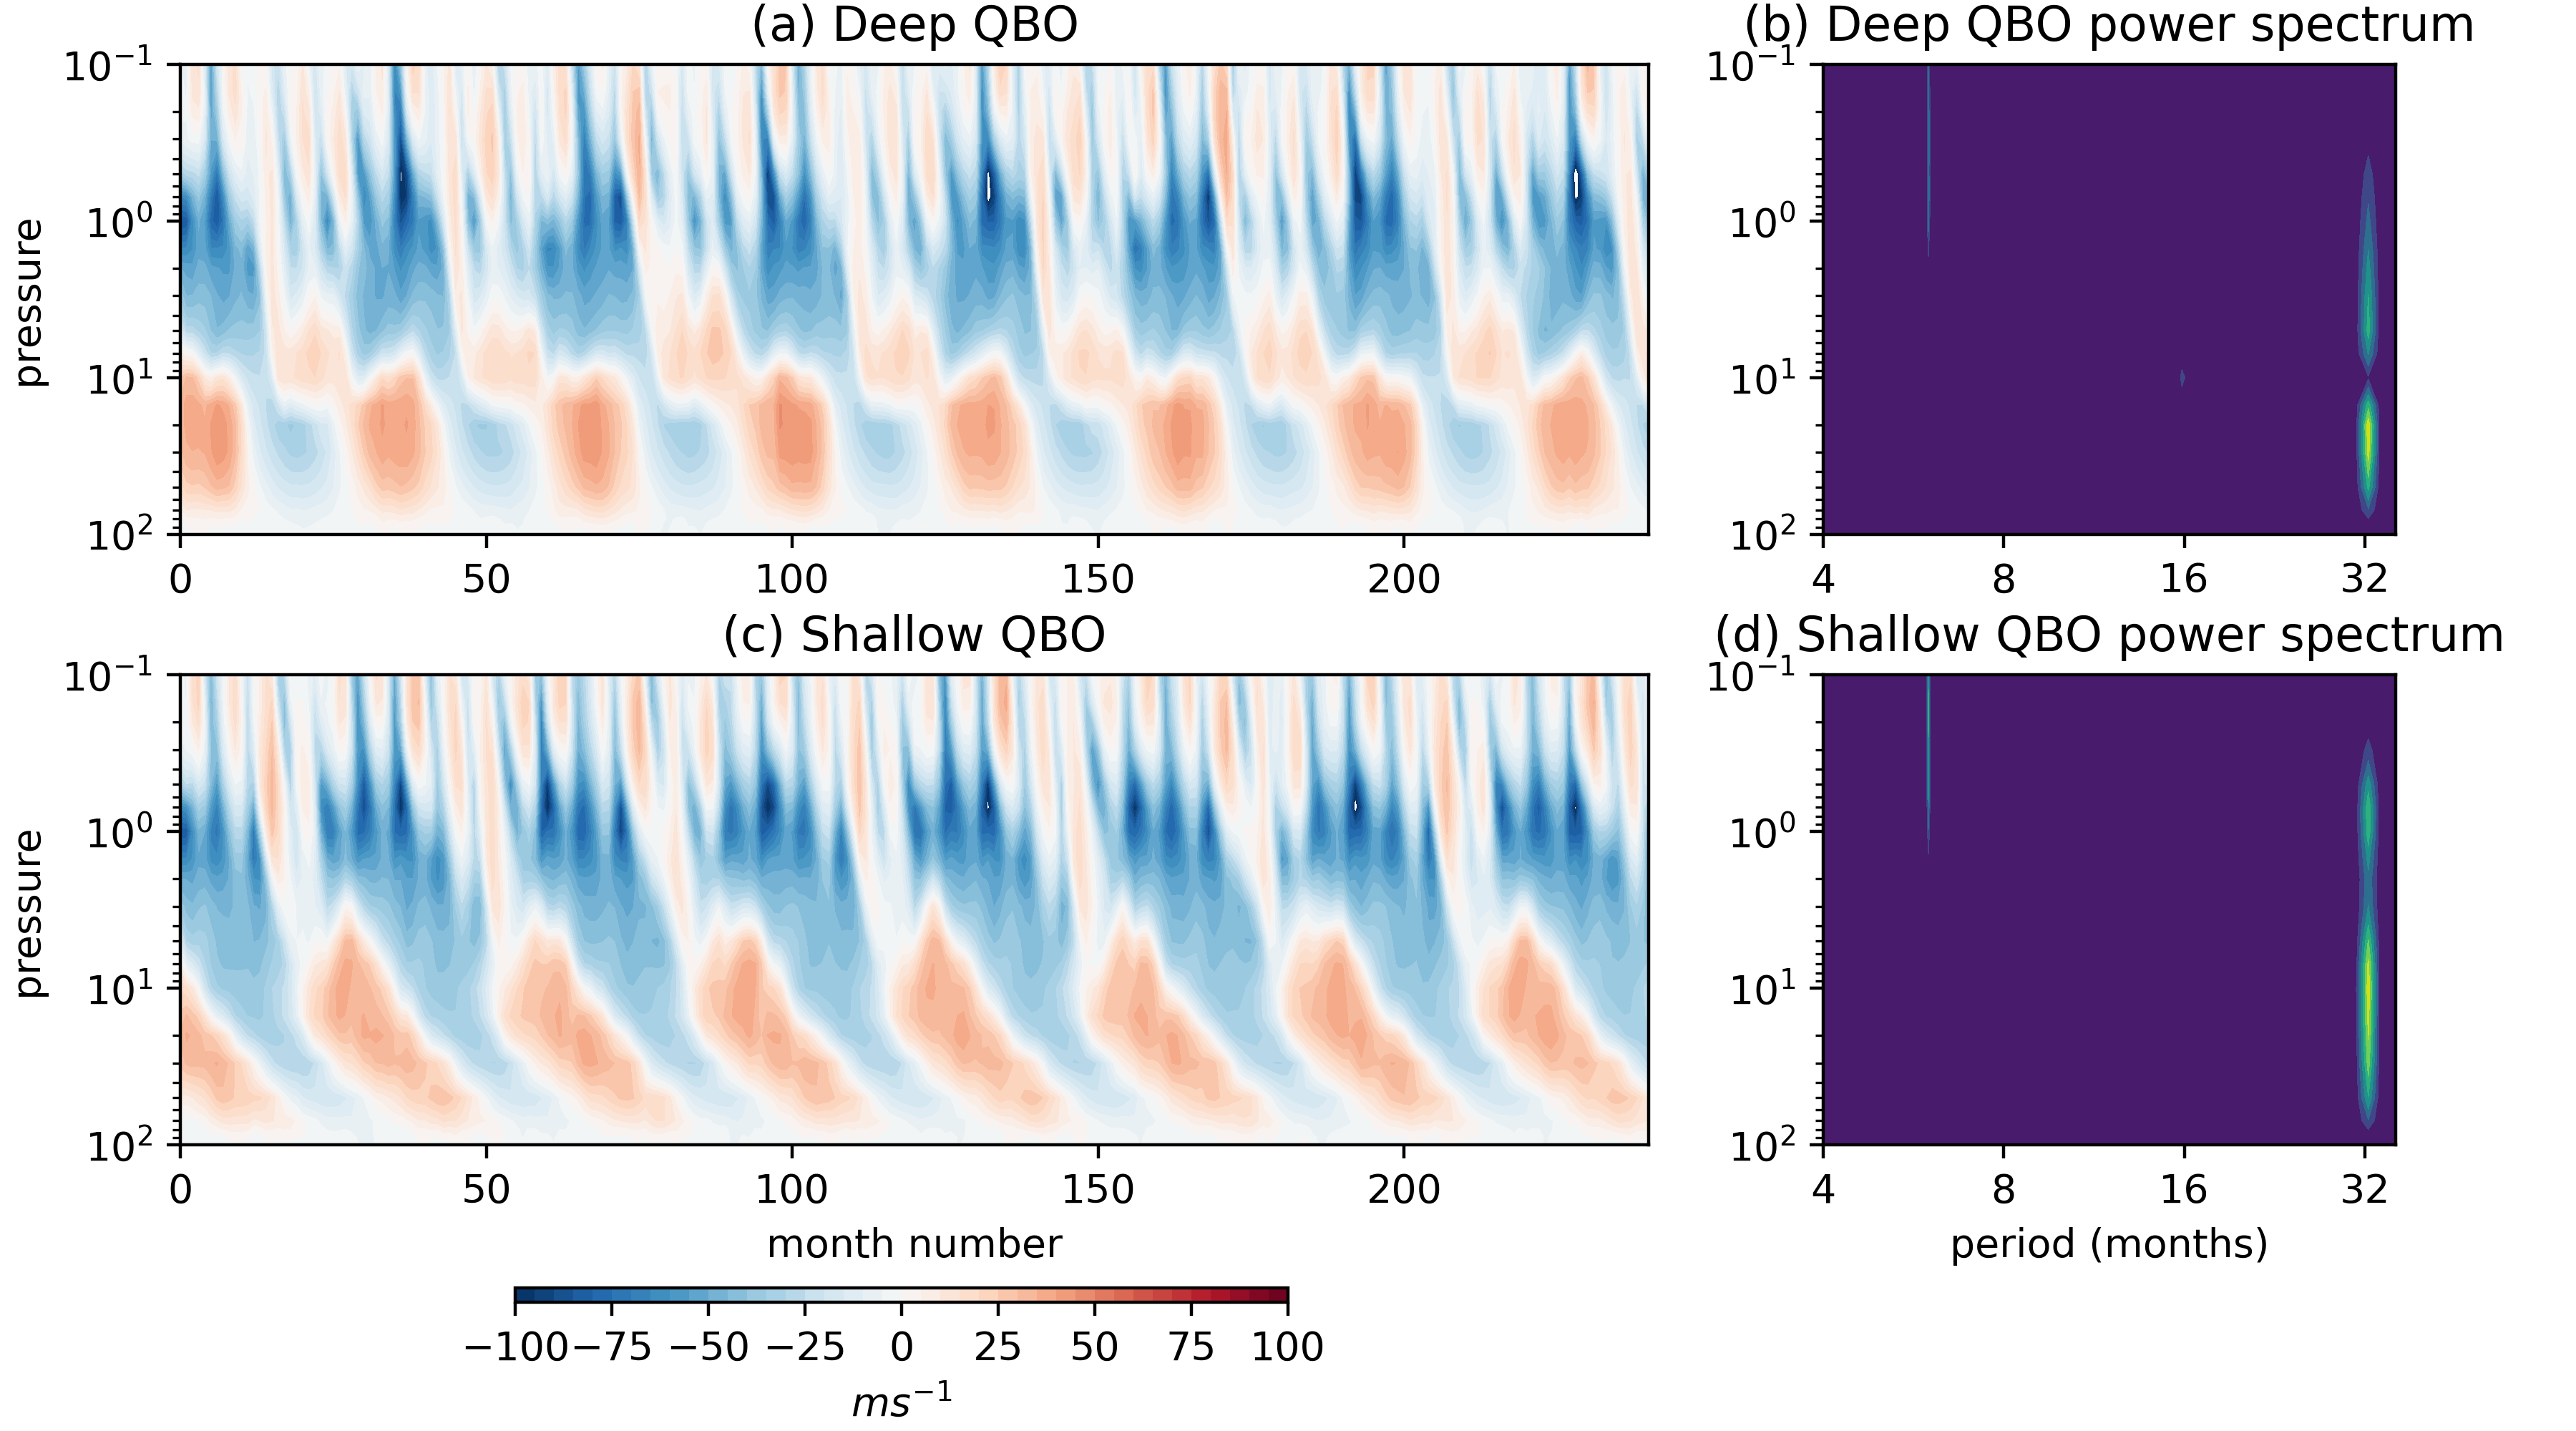
\includegraphics[width = \linewidth]{Figures/Figures-deepQBO/experiment_QBOs.png}
\caption[Equatorial ZMZW time-height profiles from QBO nudging experiments]{20 year sample of ZMZW averaged between 5$^{\circ}$\,S--5$^{\circ}$\,N latitude from the deep (\textbf{a}) and shallow (\textbf{c}) QBO experiments. Horizontal dashed lines on (a) and (c) denote the xxhPa and 90hPa pressure levels between which we implement nudging towards the idealised wind in each experiment.}
\label{fig:experiment_QBOs}
\end{center}
\end{figure}


on inspection, the time-height profile from the deep experiment is irregular. 

there are a set of discontinuities occuring at the 10hPa level where the nudging boundary is situated.

\begin{figure}[h!]
\begin{center}
\noindent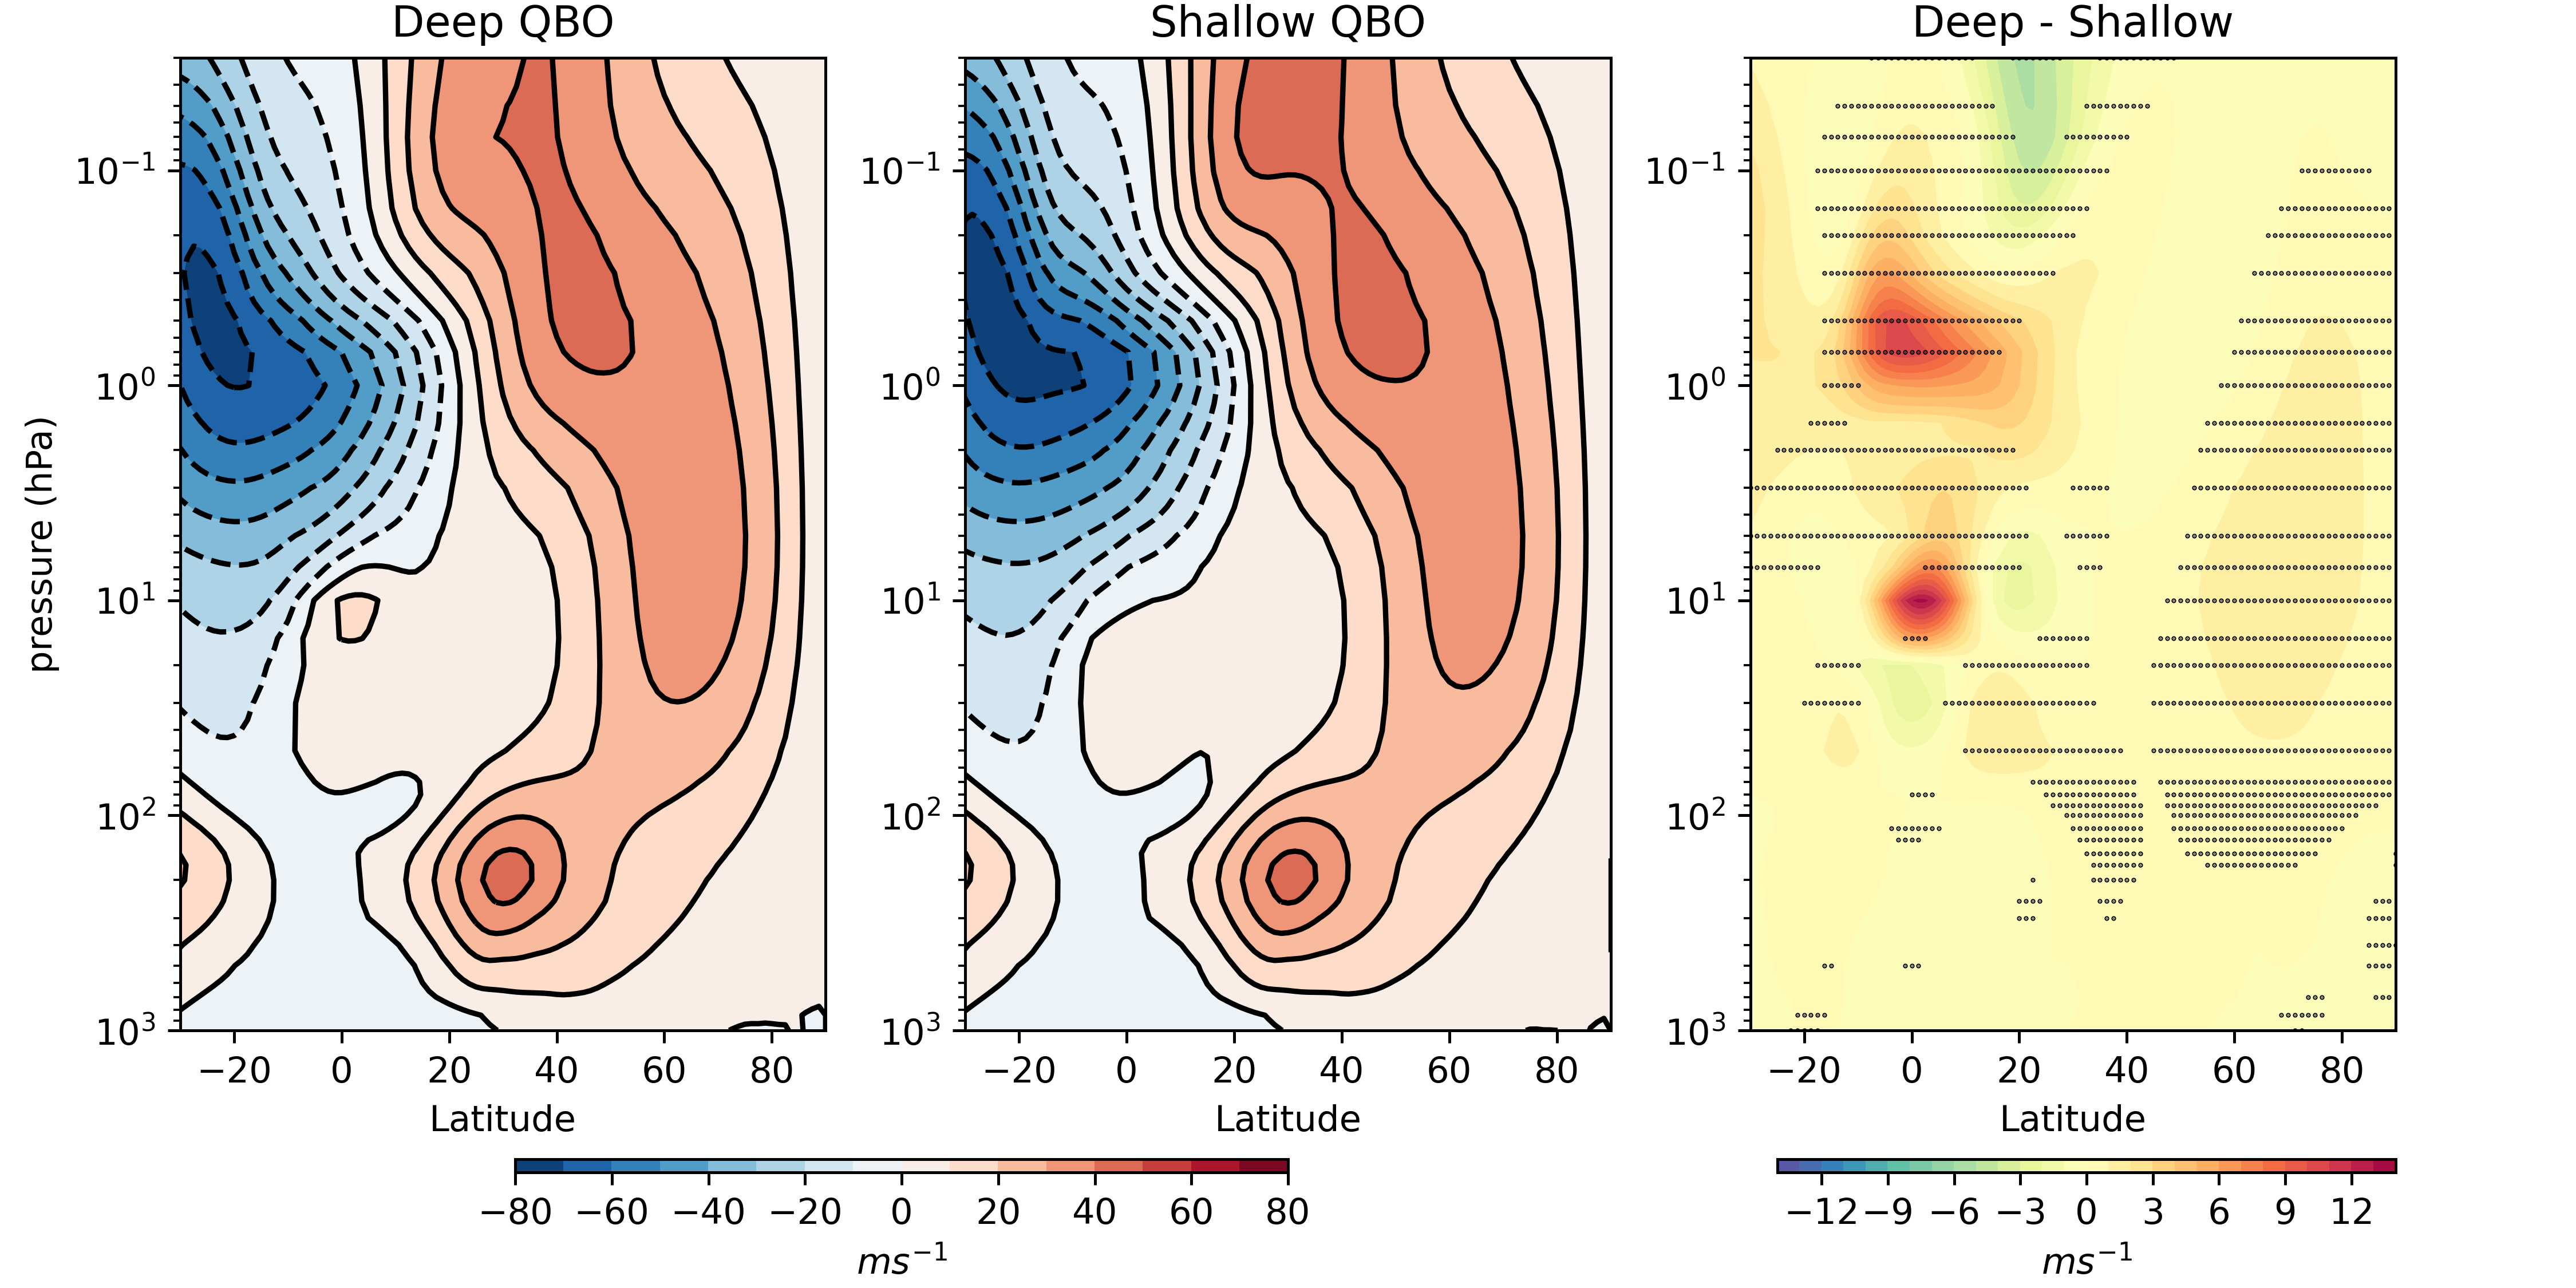
\includegraphics[width = \linewidth]{Figures/Figures-deepQBO/DJF_climatologies.png}
\caption[Equatorial ZMZW time-height profiles from QBO nudging experiments]{20 year sample of ZMZW averaged between 5$^{\circ}$\,S--5$^{\circ}$\,N latitude from the deep (\textbf{a}) and shallow (\textbf{c}) QBO experiments. Horizontal dashed lines on (a) and (c) denote the xxhPa and 90hPa pressure levels between which we implement nudging towards the idealised wind in each experiment.}
\label{fig:climatologies_experiments}
\end{center}
\end{figure}


\begin{figure}[h!]
\begin{center}
\noindent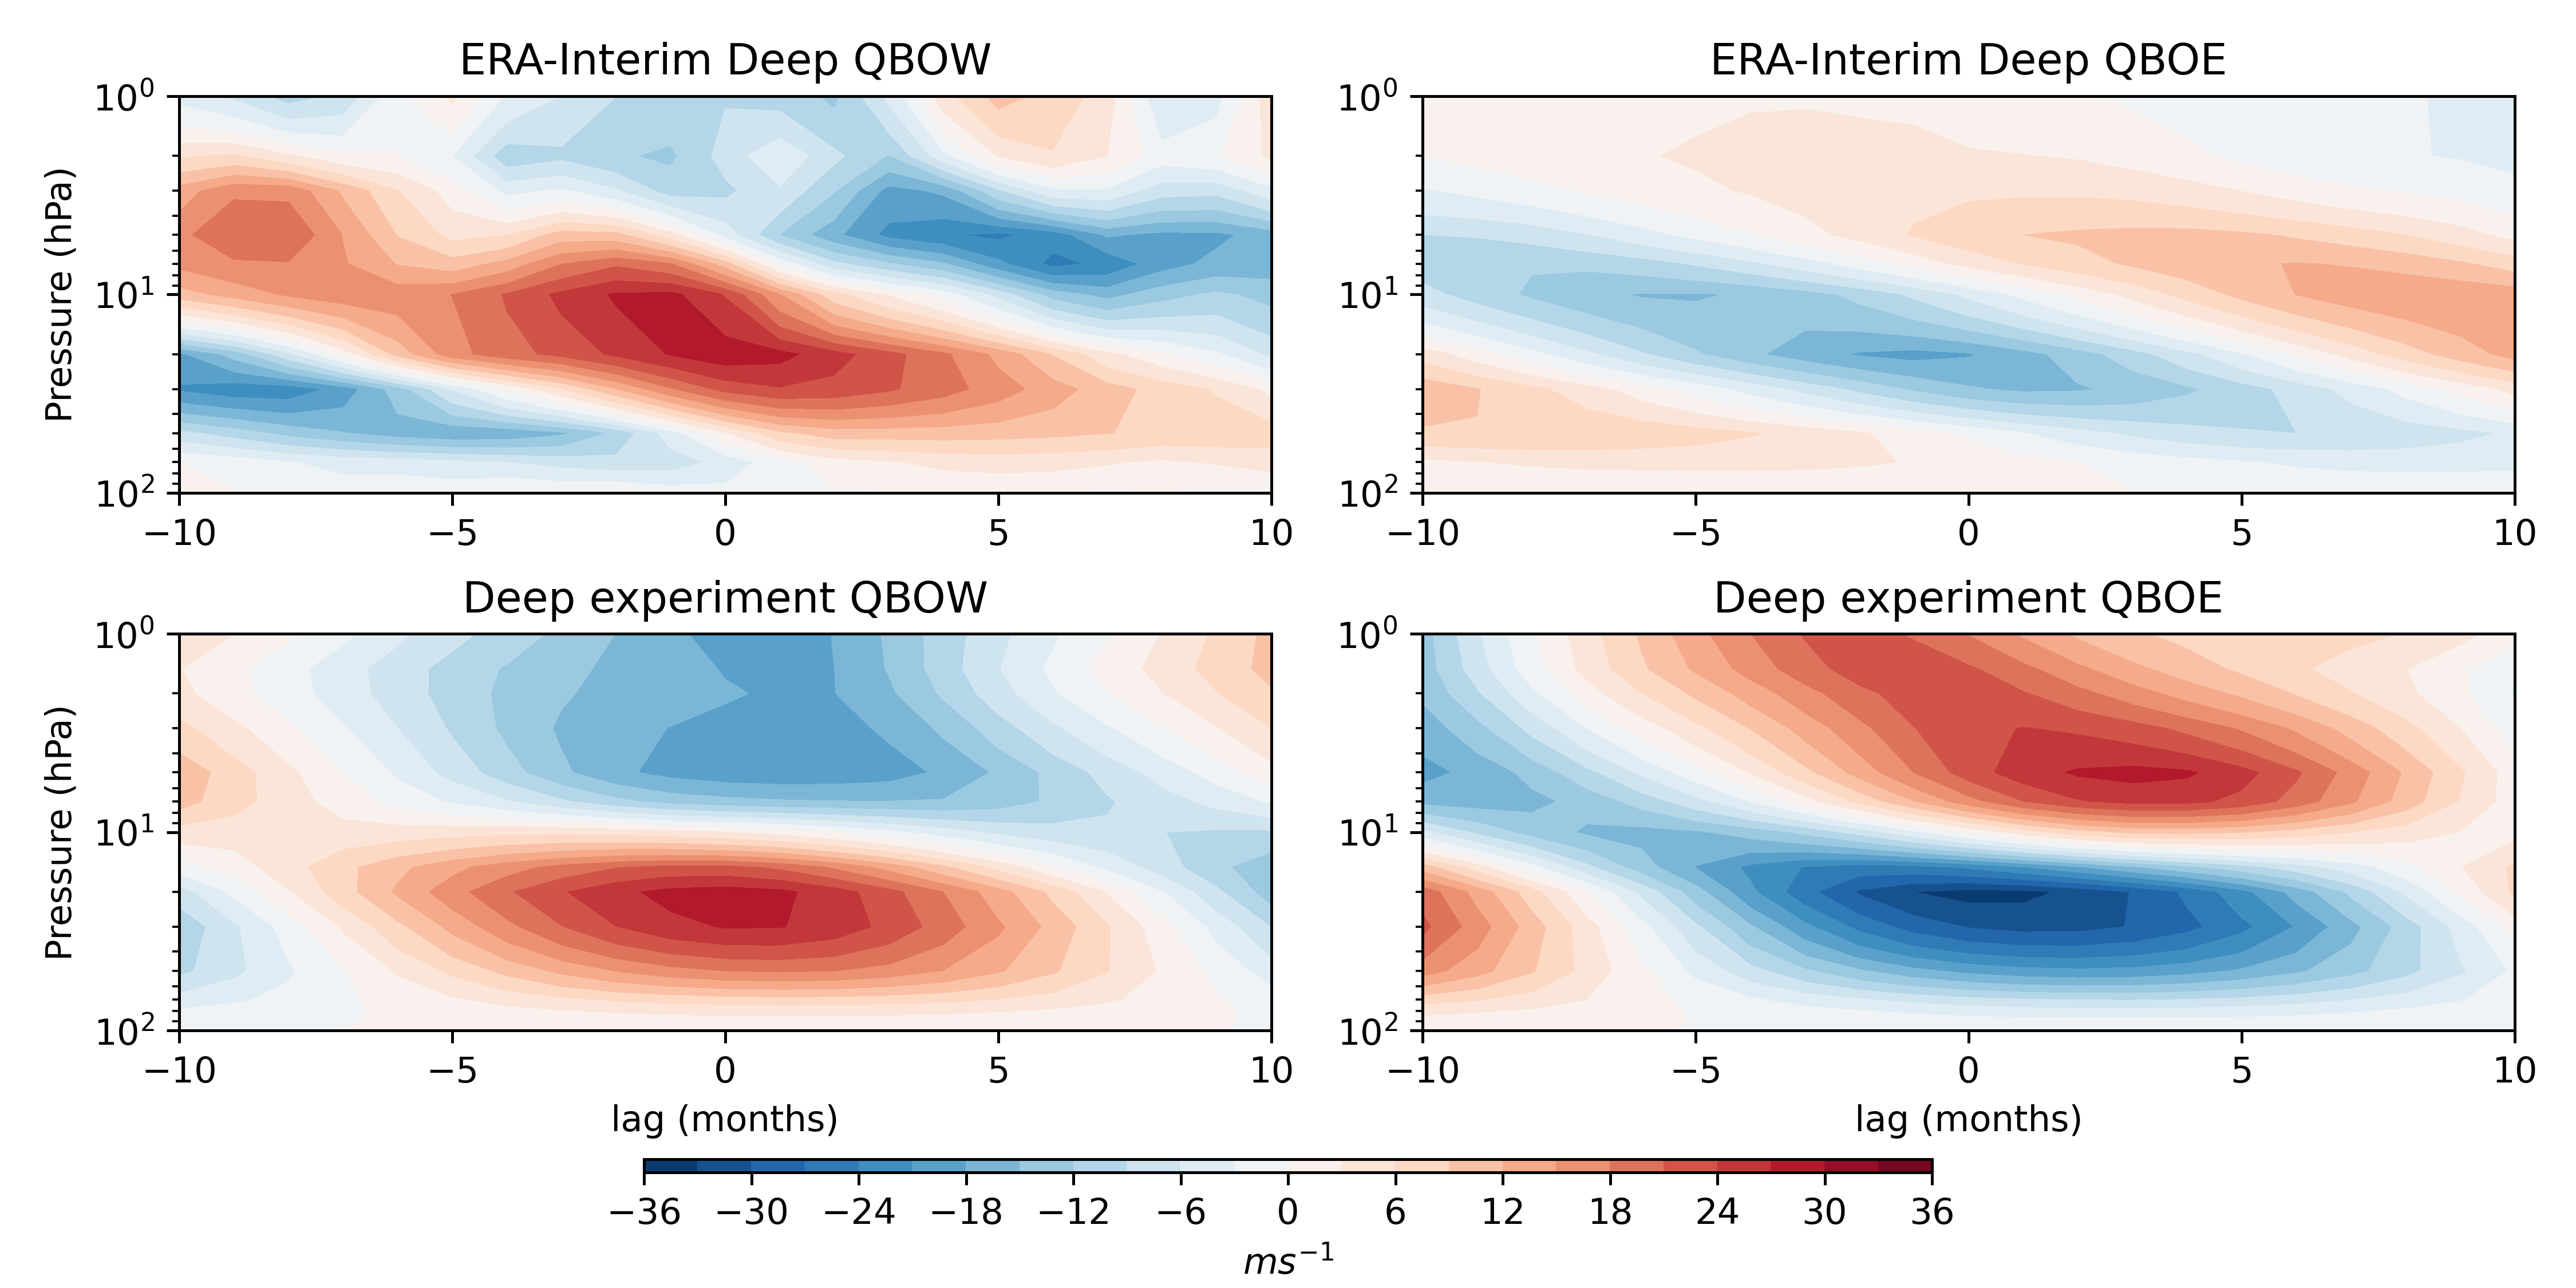
\includegraphics[width = \linewidth]{Figures/Figures-deepQBO/deep_composites_ERA_deepexp.png}
\caption[Equatorial ZMZW time-height profiles from QBO nudging experiments]{20 year sample of ZMZW averaged between 5$^{\circ}$\,S--5$^{\circ}$\,N latitude from the deep (\textbf{a}) and shallow (\textbf{c}) QBO experiments. Horizontal dashed lines on (a) and (c) denote the xxhPa and 90hPa pressure levels between which we implement nudging towards the idealised wind in each experiment.}
\label{fig:experiment_QBOs}
\end{center}
\end{figure}


\subsection{Upper Atmosphere Characteristics}

The equatorial winds shown in figure \ref{fig:experiment_QBOs} indicate that, in addition of variations in winds in the QBO region (between 100hPa and 10hPa), both experiments also exhibit variations in the SAO region (above the 1hPa level). Additionally, previous work suggest a key role for this region in equator-vortex teleconnections (brown et al.) and influence of the QBO state on SAO conditions (ref). As each experiment imposes significantly different QBO states, this mesospheric region may play a key role in accounting for differences in QBO teleconnections across the experiments. Figure \ref{fig:experiment_SAOs} shows the climatological seasonal cycle of upper stratospheric and lower mesospheric winds in each experiment - a measure of the strength of each phase of the SAO. 

\begin{figure}[h!]
\begin{center}
\noindent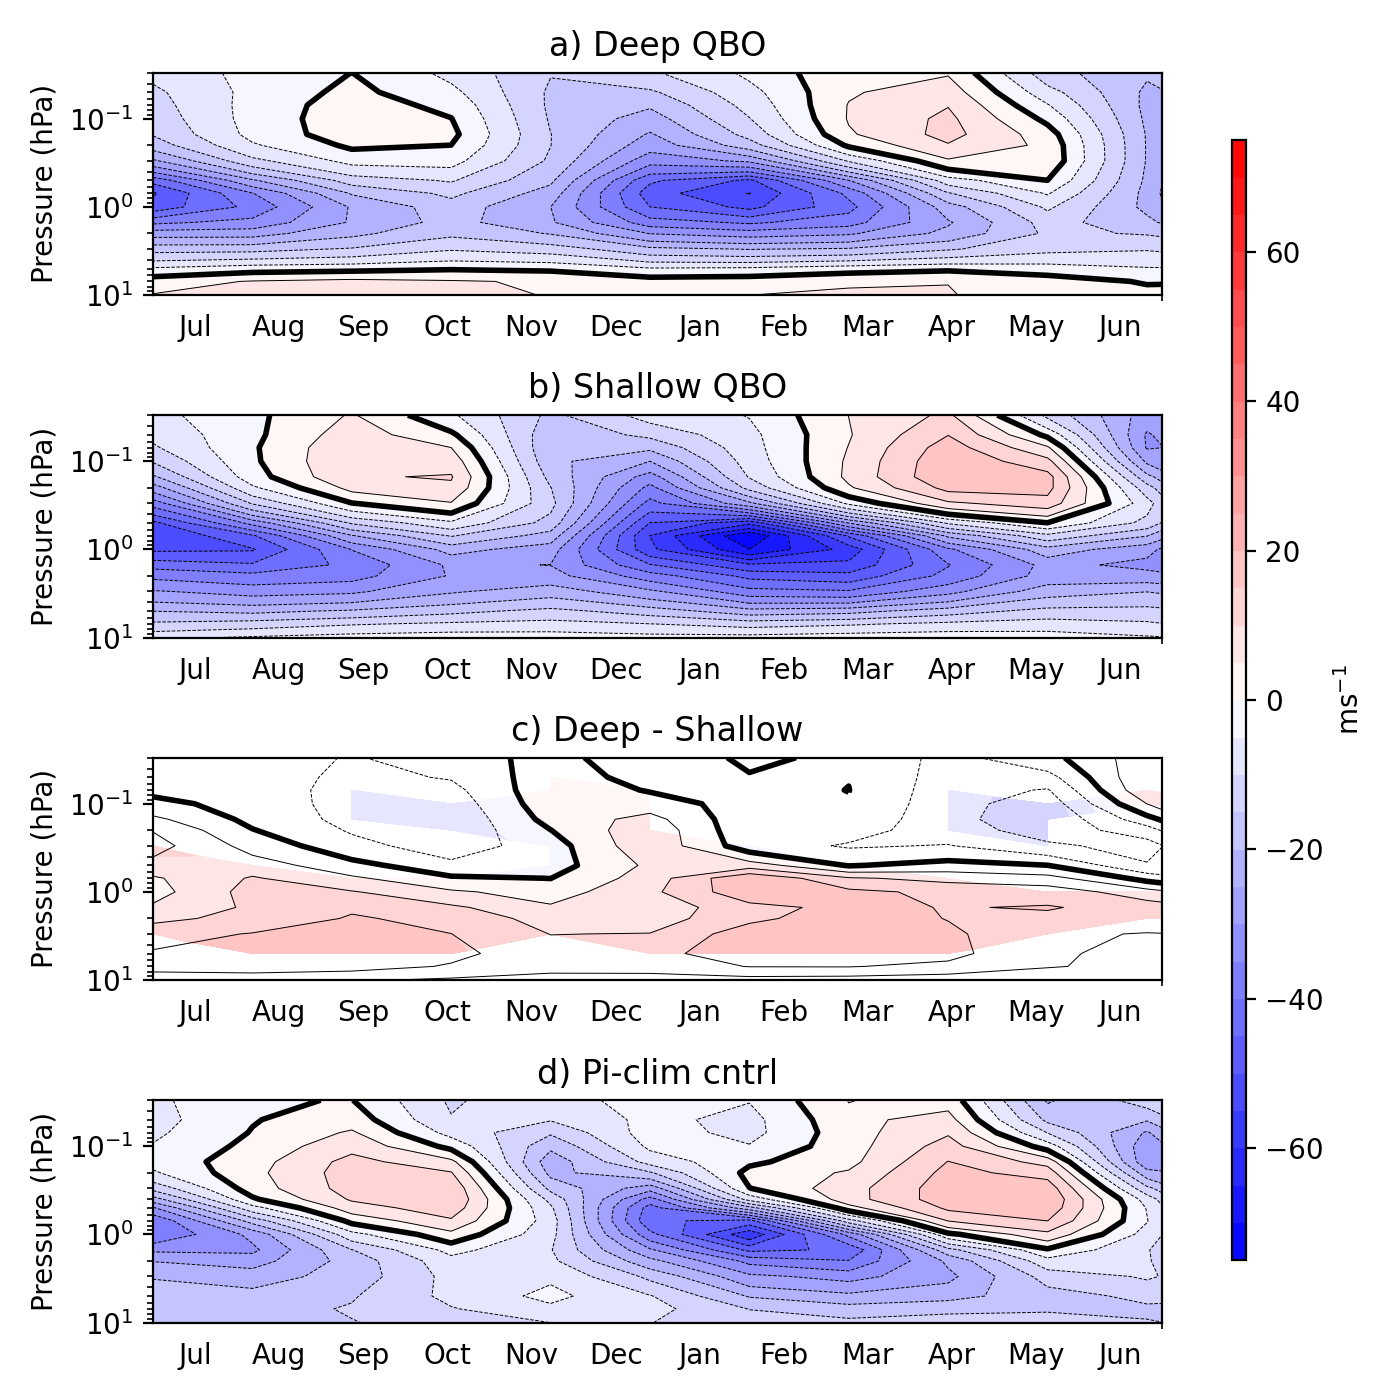
\includegraphics[width = 0.7\linewidth]{Figures/Figures-deepQBO/SAO_seasonal_cycles.png}
\caption[Climatological seasonal cycle of equatorial ZMZW in QBO experiments]{Climatological seasonal cycle of ZMZW averaged between 5$^{\circ}$\,S--5$^{\circ}$\,N latitude from the deep (\textbf{a}) and shallow (\textbf{b}) QBO experiments. Panel \textbf{c} shows climatological differences between deep and shallow seasonal cycles. Black dots on (c) denote differences significant to the 95\% level under a 2-tailed student's t-test.}
\label{fig:experiment_SAOs}
\end{center}
\end{figure}


\subsection{QBO teleconnections}

\begin{figure}[h!]
\begin{center}
\noindent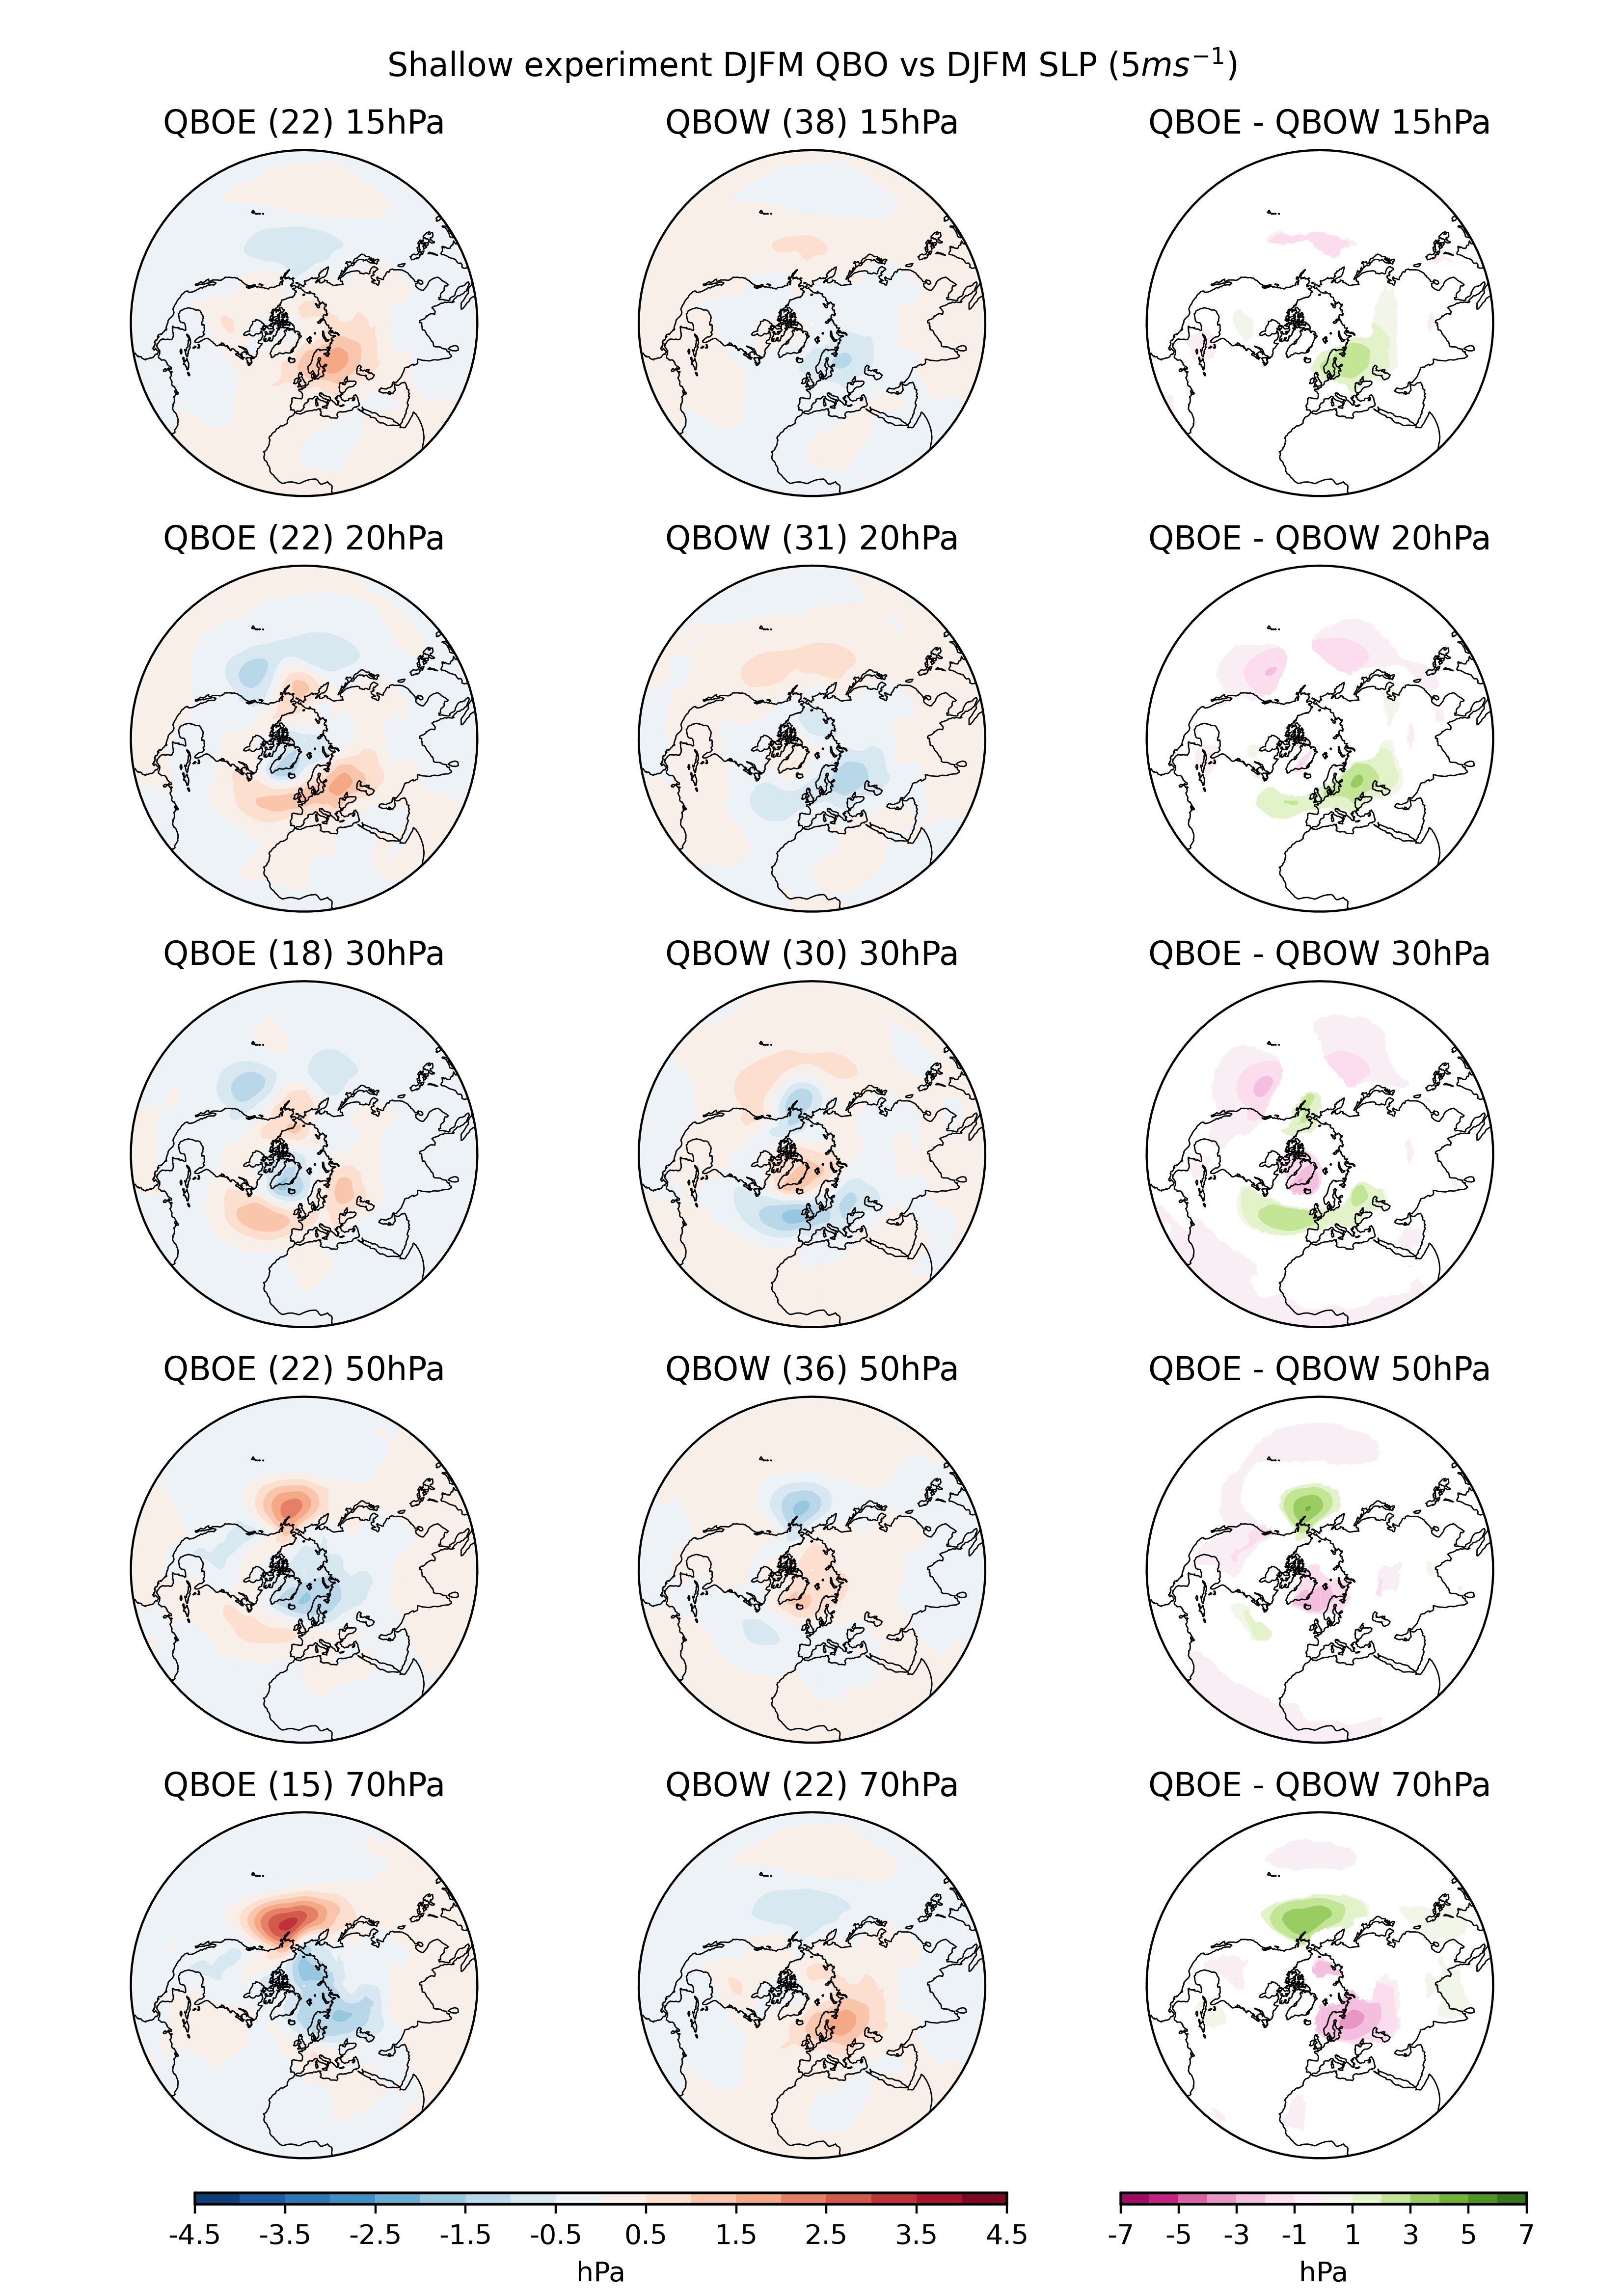
\includegraphics[width = \linewidth]{Figures/Figures-deepQBO/SLP_composites_QBO_phases_s_DJFMQBO_vs_DJFM_70hPa_5thresh.png}
\caption[Climatological seasonal cycle of equatorial ZMZW in QBO experiments]{Climatological seasonal cycle of ZMZW averaged between 5$^{\circ}$\,S--5$^{\circ}$\,N latitude from the deep (\textbf{a}) and shallow (\textbf{b}) QBO experiments. Panel \textbf{c} shows climatological differences between deep and shallow seasonal cycles. Black dots on (c) denote differences significant to the 95\% level under a 2-tailed student's t-test.}
\label{fig:experiment_SAOs}
\end{center}
\end{figure}


\begin{figure}[h!]
\begin{center}
\noindent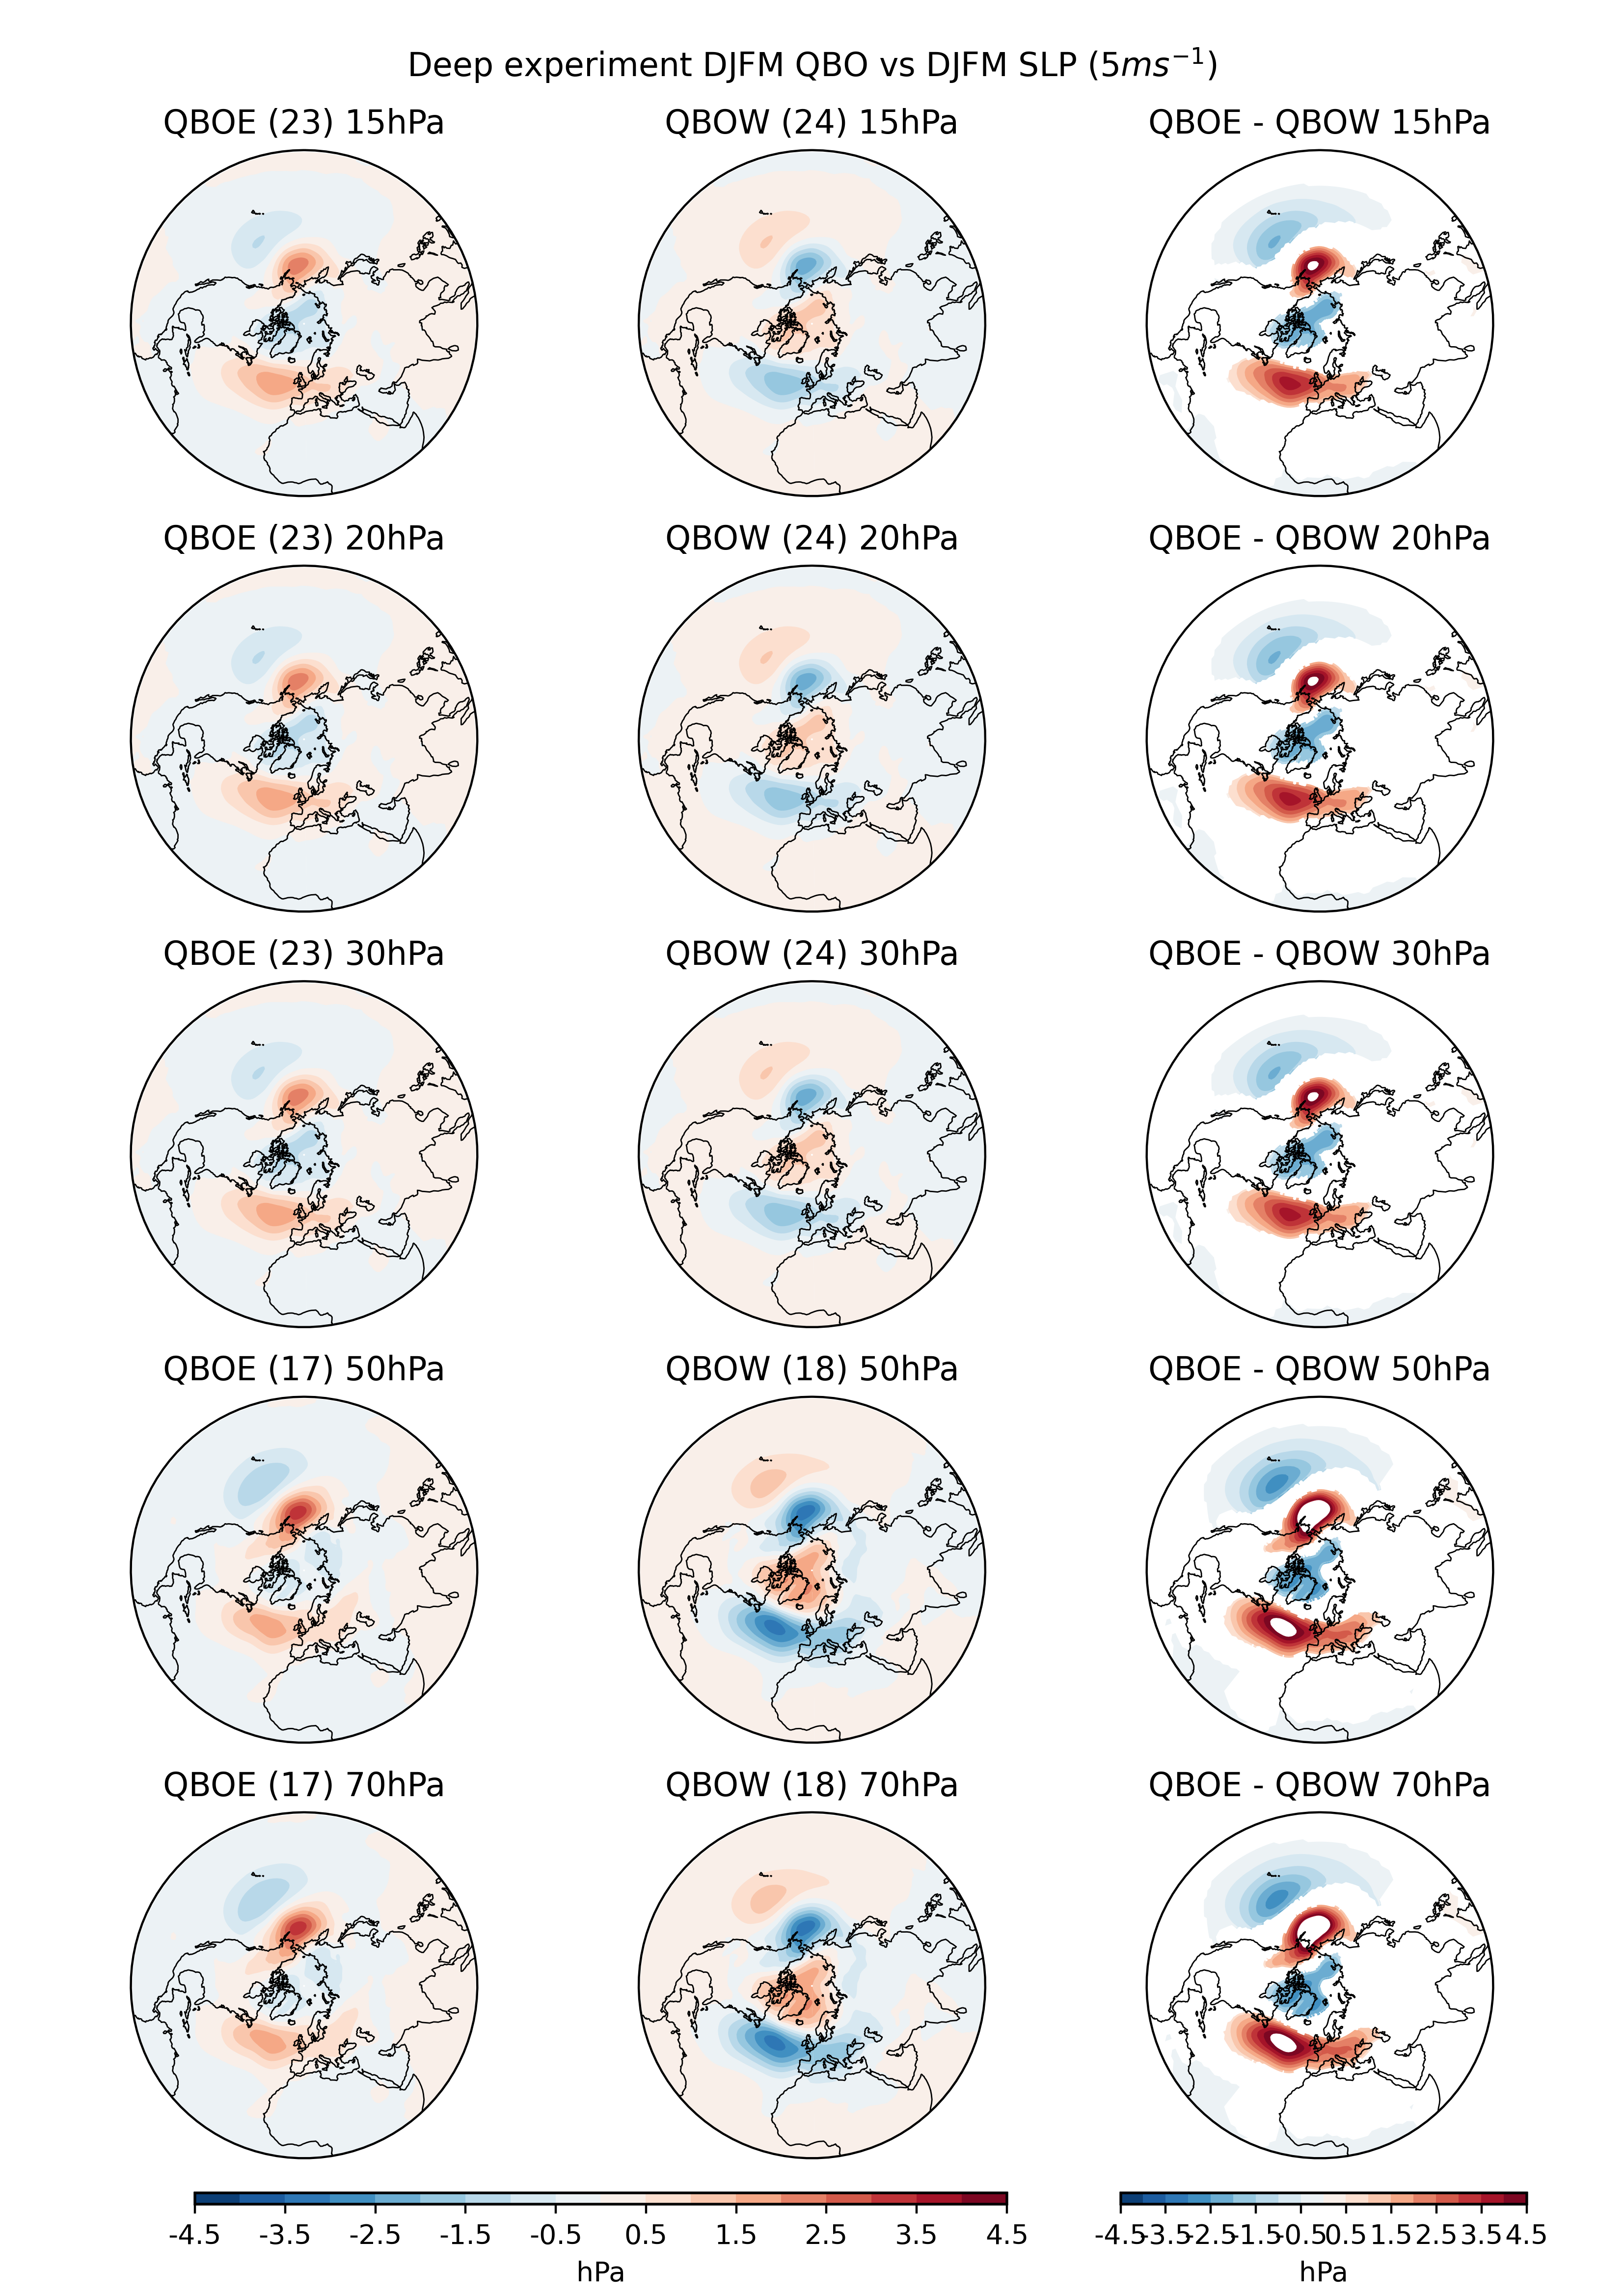
\includegraphics[width = \linewidth]{Figures/Figures-deepQBO/SLP_composites_QBO_phases_d_higher_DJFMQBO_vs_DJFM_70hPa_5thresh.png}
\caption[Climatological seasonal cycle of equatorial ZMZW in QBO experiments]{Climatological seasonal cycle of ZMZW averaged between 5$^{\circ}$\,S--5$^{\circ}$\,N latitude from the deep (\textbf{a}) and shallow (\textbf{b}) QBO experiments. Panel \textbf{c} shows climatological differences between deep and shallow seasonal cycles. Black dots on (c) denote differences significant to the 95\% level under a 2-tailed student's t-test.}
\label{fig:experiment_SAOs}
\end{center}
\end{figure}



\chapter{Conclusions}
\label{cha:conclusions}

\section{Summary of results}

The main findings of this thesis are summarised as follows: 
%\begin{enumerate}

\paragraph{Multi-decadal variations in polar vortex strength:}
While most works focus on seasonal effects of vortex variability, their non-uniform distribution in time in reanalysis datasets suggests the possibility of longer term variations. We showed that, in a pi-control integration of a GCM (UKESM), the strength of the vortex exhibits spectral power on timescales between 30 and 100 years. This power is particularly apparent when the vortex index, either in the form of an event-based SSW time series (as is analysed in chapter 3) or a continuous metric (e.g. the NAM$_{10}$, chapter 4), is smoothed to capture the occurrences of intervals of consecutive NH winters exhibiting the same type of anomalous behaviour. These signals are highly non-stationary with the most persistent spectral feature appearing for approximately 450 years on the $\sim$90-year timescale. 

\paragraph{Drivers of multi-decadal variability in the vortex:}
We identified co-variations between 90-year period signals in vortex variability with amplitude variations in a deep QBO metric. The deep QBO metric was defined by taking the average equatorial wind between 15 hPa and 30 hPa and identifies NH winters during which the vertical structure of the QBO is anomalously coherent (i.e. showing agreement in phase across pressure levels). Amplitude variations appear most pronounced in the westerly phase of the QBO and exhibit the most coherent behaviour with the appearance of hiatus intervals of SSWs. This association is consistent with the well-studied Holton-Tan relationship in which the presence of the westerly QBO phase in NH winter leads to greater latitudinal dispersion of vertically propagating planetary wave activity and subsequently a stronger vortex. The vortex indices exhibited minimal co-variability with major modes of surface variation on multi-decadal timescales and wavelet spectra for ENSO and the AL fail to account for large portions of the SSW and NAM wavelet power spectra on these multi-decadal timescales.

\paragraph{Surface influence of multi-decadal vortex variability:}
We analysed possible influences of multi-decadal signals in the vortex on tropospheric, surface and ocean variability with a particular focus on the Atlantic sector given the timescales involved (which were similar to the AMOC's characteristic periods) as well as the in-season association between the vortex and this region. We found that intervals of approximately 6-8 years that exhibit persistent anomalous vortex behaviour were found to lead to oscillatory responses in the Atlantic Meridional Overturning Circulation (AMOC) which were mediated through feedbacks with variations in ocean-atmosphere heat fluxes and the NAO. These AMOC responses peak in magnitude at lags of 2-3 years and $\sim$17 years following the vortex anomalies and were also characterised by non-stationary variations at periods of 30 and 50 years in the vortex, NAO and AMOC. We also found that the AMOC varies on longer timescales, similar to the 90-year vortex variability, but power at this periodicity was not present in the NAO suggesting that mechanisms on these longer timescales may be different to those at 50 and 30-year periods. 

\paragraph{AMOC influence on the QBO:}
We subsequently analysed possible sources of this 90-year variability of amplitude modulation in the deep QBO to determine whether variations were internally generated in the atmosphere or driven by low-frequency surface modes. While indices of major surface variation such as ENSO and the AL failed to account for large parts of the QBO and vortex wavelet spectra, significant co-variations between the QBO amplitude and deep convection indices over the eastern Pacific region were found. This co-variation supports the hypothesis that tropical upwelling and deep convection influence the vertical structure of the QBO and hence the formation of a deep QBO structure, providing a source of 90-year oscillations in the vortex from the surface. Co-variability between the AMOC and East Pacific deep convection was also shown at 90-year periods and AMOC variability on this timescale was distinct to that at 50 and 30-year periods as it is not accompanied by similar NAO variations. This result suggests a physical pathway by which 90-year timescale variations in the AMOC influence the vortex via modulation of tropical east pacific convection and modulation of the deep QBO amplitude. 

\paragraph{Stratospheric role in recent AMOC trends:}
Using the lagged response of the AMOC to anomalous vortex intervals in the UKESM pi-control simulation, we estimated the potential contribution to recent observed trends in the AMOC from the interval of anomalously strong vortex winters in the 1990s. We found that the magnitude of the filtered NAM$_{10}$ extremes in the model, which captures both the strength and persistence of the vortex anomaly, was directly proportional to the AMOC anomaly 17 years later with a remarkable degree of correlation (r = -0.908). Furthermore, using this estimation of the lag yielded an estimate of the stratospheric contributions to the AMOC downturn between 2004 and 2012 of $-0.89Sv$ at 50$\degree$N ($-0.5Sv$ at 30$\degree$N). This contribution represents approximately 30\% (17\% at 30$\degree$N) of the total negative trend and suggests a key role for the vortex, a mode of internal variability, in driving observed AMOC variations. 

\paragraph{Importance of QBO vertical structure in teleconnections:}
We designed a set of nudging experiments to explicitly test the influence of vertical coherence in the QBO on the strength of teleconnections with the vortex and the surface (the AO and NAO).

The QBO responses of the deep experiment were dominated by large amplitude anomalies in the vortex and MSLP with QBOE(W) phases associated with a stronger (weaker) vortex and positive NAO and AO patterns. These are of the opposite sign to an expected HT link as well as the results of similar previous works \citep{graySurface2018b, andrewsObserved2019d}. We found that these unexpected responses were associated with large amplitude anomalies in the SAO region likely caused by preferential filtering of equatorial waves by the deep QBO phase below. These equatorial USLM winds were associated with significant anomalies in vortex strength, consistent with a possible influence from this region. However, the design of the idealised deep QBO experiment resulted in a simple two/three-fold vertical structure of the equatorial QBO, which is unrealistic. The influence from the USLM may therefore have been over-estimated in this experiment.

Examination of the HT relationship using a deep QBO metric in the 1000-year UKESM pi-control simulation showed a more realistic four-fold vertical QBO structure, as well as the correct sign of the HT relationship and MSLP response. The analysis of this simulation showed a consistent HT - vortex - Atlantic MSLP relationship, confirming the likely role of the polar route for stratospheric influence on the NAO via vortex variations, but also identified a possible contribution to both the Atlantic and Pacific MSLP response via a subtropical route, where the induced meridional QBO circulation influences the lowermost stratosphere.  

We therefore concluded that, while the deep QBO experiment confirmed a possible influence of the deep QBO from the equatorial USLM, its design obscured the response from other height regions. The analysis highlights the complexity of the QBO influence on both vortex and surface variability and suggests that the observed QBO influence at the surface is likely to be the result of a combination of processes that involve different height regions of the equatorial atmosphere.  

\section{Limitations and further investigations}
\label{sec:limitations}
The work presented in this thesis has also raised a number of questions, and its limitations motivate further investigation. Some of these ideas are discussed below:

\paragraph{Determining causality in teleconnections:}
While time series analyses such as those presented in chapters 3 and 4 can highlight associations between key modes of climate variability, they are less effective at determining causality in connections. Where possible, we have selected indices that confirm well-known in-season causality, such as an early winter QBO index compared with a mid-winter SSW index (as in chapter 3) or the vortex impact on Atlantic MSLP and subsequent links to the AMOC (chapter 4). Nevertheless, determining causality on longer timescales is difficult as the climate system is extremely complex, with many different interactions between modes of variability. These complexities can hamper simple statistical analysis such as multi-linear regression (as used in chapter 3 on SSW, QBO and surface time series) as it fails to capture the non-stationary nature of signals and suffers from the potential non-orthogonality of explanatory variables (ENSO, the QBO and the AL). While we employed more sophisticated techniques such as wavelet analysis to account for non-stationarity, establishing causal connections remains an issue.

Further work into determining causality could involve tailor-made statistical methods such as the Causal Effect Network (CEN) framework \citep{Kretschmer2016} which has been developed for the analysis of causal connections in complex systems of time series data. This method identifies connections between pairs of time-series selected from a large group of indices while filtering out spurious correlations that arise between series which are not causally linked. For example, a correlation may arise between two variables that have no direct physical link if they are both driven by the same underlying process or via autocorrelation effects \citep{rungeQuantifying2014}. Implementation of the CEN technique on indices such as those analysed in chapter 4 (the NAM$_{10}$, NAO, sub-polar North Atlantic heat flux and the AMOC) may aid in improving understanding of the physical pathways involved in interactions. For example, it may establish whether the NAO-AMOC interaction, which was shown to arise following a filtered NAM$_{10}$ extreme, is prominent in the absence of a stratospheric anomaly or if the extreme vortex behaviour is a necessary triggering mechanism. 

\paragraph{Targeted experiments:}
To overcome these issues with demonstrating causality in teleconnections, we also recommend a set of targeted sensitivity experiments using GCM simulations whose design is informed by our results. These experiments impose different multi-decadal signals on key climate indices using a similar nudging method as utilised in chapter 5 \citep{telfordTechnical2008}.

\begin{itemize}
    \item To test the connection between multi-decadal signals in QBO amplitude modulation and SSWs suggested in chapter 3, a set of simulations which impose variability in QBO amplitude: For example, one simulation could prescribe oscillating QBO amplitude on the 90-year timescales while another imposes a constant QBO amplitude. Comparison of multi-decadal signals in SSW frequency in these experiments could establish whether the signals in the pi-control (chapter 3) are causally linked.  
    
    \item Similar model setups designed to test the robustness of vortex-AMOC interactions could also be implemented. A simulation in which variability in vortex strength is imposed on decadal timescales with a pre-defined period may be appropriate in this case: Comparisons of the AMOC in such simulations with runs that imposed no decadal variability in the vortex could explicitly test the role of NAM$_{10}$ variations in multi-decadal AMOC variability. 
    
\end{itemize}

\paragraph{The true role of the stratosphere in observed AMOC trends:}
Our results regarding the role of the SSW hiatus in the 1990s in recent AMOC trends also carry a number of limitations. For example, the AMOC response to extreme NAM$_{10}$ intervals appear heavily weighted towards 30-year timescale variations. Variations on this timescale are highly non-stationary and it is unclear whether similar signals are present in the observational record, not least due to the short record of direct observations of the AMOC. Furthermore, as with the multi-decadal interactions, our analysis determined a strong statistical link between the phenomena but struggles to explicitly prove causality. Further sensitivity analysis may address some of these issues. Namely, relaxation experiments which impose an SSW hiatus interval of $\sim9$years and, at the end of this interval, allows the model to evolve freely to measure the lagged AMOC response compared to a control simulation with no stratospheric perturbation. Similar experiments which measure the response to consecutive NH winters with the same NAO pattern \citep{delworthImpact2016c} showed promising results with significant AMOC anomalies from a control simulation evident. Our proposed experiments would test whether an SSW hiatus interval provides a large enough perturbation to induce significant NAO/AMOC anomalies.

\paragraph{Limitations of a single model approach:}
The results from chapters 3 and 4 regarding the interaction between multi-decadal variations in the polar vortex and other parts of the climate system is derived from a single simulation of a single GCM - the UKESM pi-control. This poses a potentially significant issue as the model exhibits biases in its representation of some key modes of climate variability. For example, November SSWs are significantly over-represented (figure \ref{fig:SSW_histogram}) which may affect the progression of its strength through the winter as the vortex recovers from a November disruption which precludes further significant wave driving. The mean period of the QBO in the model is also longer than that exhibited by ERA-Interim \citep{bushellEvaluation2020b}. This could lead to an over-inflated HT strength due to the longer persistence of QBO phases altering the mid-latitude waveguide through, on average, a larger portion of NH winter. Finally, the model under-represents decadal-scale variation in AMOC over the historical period \citep{robsonEvaluation2020d}. 

These biases may result in teleconnections in the model that are not fully representative of the real atmosphere. Recent work has also shown a large degree of inter-model variability exists in representations of the QBO \citep{bushellEvaluation2020b} as well as SSWs \citep{ayarzaguenaUncertainty2020b} suggesting the possibility that results from our studies are model dependant. Further work could consider a suite of CMIP6 models and examine the multi-decadal signals in the vortex, QBO, NAO and AMOC to test the robustness of the various teleconnections established in the analysis of this thesis.   

\paragraph{More effective QBO nudging:}
In chapter 5, we designed a set of nudging experiments which relaxed the QBO winds towards idealised fields (the deep and shallow QBO). However, a comparison of these fields with the model winds (figures \ref{fig:winds_on_levs_deep} and \ref{fig:winds_on_levs_shallow}) revealed the westerly phase of the QBO is under-represented in the model output despite the applied relaxation. This problem was particularly prevalent when nudging towards a deep QBO and poses potential issues with future QBO studies as it leads to significant asymmetries in nudged QBO phases.

Further analysis into rectifying this bias could involve a set of sensitivity experiments that implement nudging of the QBO towards the same idealised fields using smaller values for nudging timescales ($\tau$ in equation \ref{eq:nudging}) than we used in our experiments ($\tau$ = 6 hours). $\tau$ is generally set to 6 hours in line with the temporal resolution of reanalysis files commonly used for nudging (and is similar to that used in other families of models) \citep{telfordTechnical2008} however, using idealised fields, which can be generated at any temporal resolution, removes this constraint. Assessing the reduction in QBO bias achieved by reducing $\tau$ as well as the possible model instability introduced by using a short nudging timescale, could aid in implementing more effective QBO nudging in future studies.

\paragraph{Constraining the USLM QBO:}
While our QBO experiments successfully imposed a deep and shallow QBO in the lower-mid stratosphere (figure \ref{fig:experiment_QBOs}), the deep experiment induced large anomalies in the equatorial USLM region (figure \ref{fig:HT_deep}). These anomalies were shown to lead to large vortex and surface responses of the opposite sign to the expected HT link as well as the results of \cite{andrewsObserved2019d}. This USLM QBO signal obscured other possible physical pathways associated with the QBO and prevented a definitive evaluation of the role of vertical coherence in QBO teleconnections. 

To analyse other possible pathways closer, we recommend further simulations which impose a deep QBO in the lower and mid stratosphere and also nudges the SAO winds. In the SAO region, winds could be nudged towards climatological values calculated from another simulation (the pi-clim cntrl, for example) in order to remove the large anomalies induced by the deep QBO in our experiment. Eradicating the influence of these USLM responses may aid in isolating the influence from other height regions involved in QBO teleconnections, including the potential influence from the induced meridional QBO circulation via the subtropical route described in \cite{graySurface2018b}. Isolation of these other effects may develop a better understanding of the mechanisms at play in the presence of a vertically coherent QBO.  


















%now enable appendix numbering format and include any appendices
%\appendix
%\nclude{appendix1}
%\nclude{appendix2}


\baselineskip=14pt plus4pt % as HA
%next line adds the Bibliography to the contents page
\addcontentsline{toc}{chapter}{Bibliography}
%uncomment next line to change bibliography name to references
%\renewcommand{\bibname}{References}
\bibliography{bibliography_improved}        %use a bibtex bibliography file refs.bib
%\bibliographystyle{plain}  %use the plain bibliography style

\end{document}

